% \documentclass{article}
\documentclass[10pt,logo,copyright]{nvidiatechreport_zh}
\linespread{1.15}

% \usepackage[authoryear,sort&compress,round]{natbib}


\usepackage{iftex}
\ifXeTeX
\else
  \usepackage[utf8]{inputenc} % allow utf-8 input
  \usepackage[T1]{fontenc}    % use 8-bit T1 fonts
\fi

% Allow URLs to break at more characters (fixes overfull hbox in bibliography)
\makeatletter
\g@addto@macro{\UrlBreaks}{\UrlOrds}
\makeatother

\usepackage{parskip}        % no paragraph indents
\usepackage{url}            % simple URL typesetting
\usepackage{booktabs}       % professional-quality tables
\usepackage{amsfonts}       % blackboard math symbols
\usepackage{nicefrac}       % compact symbols for 1/2, etc.
\usepackage{microtype}      % microtypography
\usepackage{xcolor}         % colors
\usepackage{listings}       % code listings with syntax highlighting
\usepackage{graphicx}
\usepackage{animate}        % for 360 video in teaser
\usepackage{subcaption}
\usepackage{tabularx}
\usepackage{makecell}
\usepackage{adjustbox}
\usepackage{setspace}
\newcolumntype{M}[1]{>{\centering\arraybackslash}m{#1}}
\usepackage{float}
\usepackage{tikz}
\usepackage{amsmath,amsfonts,bm, bbm,leftindex}
\usepackage{multirow}
\usetikzlibrary{arrows.meta, positioning, fit}
\usepackage{wrapfig}
\usepackage[stable,bottom]{footmisc}

% Custom NOTE environment for practical insights
\usepackage[most]{tcolorbox}
\definecolor{nvidiagreen}{RGB}{118, 185, 0}
\newtcolorbox{notebox}{
  enhanced,
  breakable,
  colback=nvidiagreen!8,
  colframe=nvidiagreen,
  boxrule=0pt,
  leftrule=3pt,
  arc=0pt,
  outer arc=0pt,
  left=10pt,
  right=10pt,
  top=8pt,
  bottom=8pt,
  before skip=\baselineskip,
  after skip=\baselineskip,
  fonttitle=\bfseries,
  coltitle=nvidiagreen!80!black,
  attach title to upper={\par\smallskip},
  title={说明}
}

% Configure listings package for code blocks
\lstset{
    basicstyle=\small\ttfamily,
    breaklines=true,
    frame=single,
    backgroundcolor=\color{gray!10},
    keywordstyle=\color{blue},
    commentstyle=\color{green!50!black},
    stringstyle=\color{red},
    numbers=none,
    xleftmargin=2em,
    framexleftmargin=1.5em,
    captionpos=b
}

% Custom environment for ASCII diagrams (non-verbatim)
\newtcolorbox{asciibox}[1][]{
  enhanced,
  breakable,
  colback=gray!5,
  colframe=gray!40,
  boxrule=0.5pt,
  arc=2pt,
  left=6pt,
  right=6pt,
  top=6pt,
  bottom=6pt,
  before skip=0.8\baselineskip,
  after skip=0.8\baselineskip,
  fontupper=\small\ttfamily,
  #1
}

% Custom style for ASCII diagrams
\lstdefinestyle{asciiStyle}{
  basicstyle=\small\fontfamily{pcr}\selectfont,
  breaklines=false,
  columns=fullflexible,
  keepspaces=true,
  frame=single,
  framerule=0.5pt,
  rulecolor=\color{gray!40},
  backgroundcolor=\color{gray!5},
  xleftmargin=8pt,
  xrightmargin=8pt,
  framexleftmargin=6pt,
  framexrightmargin=6pt,
  framesep=6pt,
  aboveskip=0.8\baselineskip,
  belowskip=0.8\baselineskip,
}

% Custom environment for ASCII diagrams (verbatim - preserves ^ and _)
\lstnewenvironment{asciiart}{\lstset{style=asciiStyle}}{}

\input{common_zh.tex}
\usepackage{graphicx} % Required for inserting images
\usepackage{amsmath} % For math symbols if needed
\usepackage{amssymb}
\usepackage{comment}
\usepackage{hyperref} % For hyperlinks if needed
\usepackage{booktabs}
\usepackage{array, booktabs, tabularx}
\usepackage{threeparttable}
\usepackage{multirow}
\usepackage{xcolor}

\newcommand{\sep}{\ensuremath{\,\cdot\,}}   % nice centred dot with thin spacing

\setcounter{secnumdepth}{3}  % number down to \subsubsection (paragraph unnumbered)
\setcounter{tocdepth}{3}     % (optional) show down to \subparagraph in TOC

% ===== Redefine section heading formats for better hierarchy =====
% Note: nvidiatechreport.cls uses titlesec with [explicit] option, so #1 is required
% Section: largest, bold
\titleformat{\section}{\Large\bfseries}{\thesection.}{0.5em}{#1}
\titlespacing*{\section}{0pt}{3.5ex plus1ex minus.2ex}{2.3ex plus.2ex}

% Subsection: large, bold
\titleformat{\subsection}{\large\bfseries}{\thesubsection.}{0.5em}{#1}
\titlespacing*{\subsection}{0pt}{3ex plus1ex minus.2ex}{1.5ex plus.2ex}

% Subsubsection: medium (between normal and large), bold
\titleformat{\subsubsection}{\fontsize{11}{13}\selectfont\bfseries}{\thesubsubsection.}{0.5em}{#1}
\titlespacing*{\subsubsection}{0pt}{2.5ex plus1ex minus.2ex}{1ex plus.2ex}

% Paragraph: normal size, bold italic, run-in (inline) style
\titleformat{\paragraph}[runin]{\normalsize\bfseries\itshape}{\theparagraph}{1em}{#1}
\titlespacing*{\paragraph}{0pt}{2ex plus.5ex minus.2ex}{1em}

% ===== Fix itemize bullets (NVIDIA font lacks proper bullet) =====
\renewcommand{\labelitemi}{\textbullet}
\renewcommand{\labelitemii}{$\circ$}
\renewcommand{\labelitemiii}{\textasteriskcentered}
\renewcommand{\labelitemiv}{\textperiodcentered}

\title{Megatron Core 上混合专家模型的可扩展训练\texorpdfstring{\\[0pt]{\large 技术报告}}{}}
% \vspace{-25pt}
\author{{\vspace{-10pt}\bfseries\large NVIDIA}\footnote{完整作者列表请参见“贡献与致谢”一节。通信作者：\texttt{\{zijiey, juney, jiajiey\}@nvidia.com}.}}

\date{\today} % Or specify a date like December 2024
\renewcommand{\contentsname}{目录}
\renewcommand{\tablename}{表}

% Remove bold formatting from abstract
\renewcommand{\absfont}{\linespread{1.15}\fontsize{10}{12}\selectfont}

% Reduce bottom margin since footer rule/copyright moved to footnote area
% \geometry{bottom=1.5cm}

% Disable footer rule and copyright from fancyhdr; copyright goes in footnote area instead
\renewcommand{\copyrightext}{}
\renewcommand{\footrulewidth}{0pt}
\renewcommand{\footrule}{}

% Reduce space between text and footnotes
\setlength{\skip\footins}{4pt}

% Replace default footnote rule with full-width colored line (NVIDIA style)
\renewcommand{\footnoterule}{\vspace*{-3pt}\noindent\textcolor{gray}{\rule{\textwidth}{1pt}}\vspace*{4pt}}

\begin{document}

% Header shows only main title (without "Technical Report" subtitle)
\fancyhead[C]{\footerfont Megatron Core 上混合专家模型的可扩展训练}
\maketitle
% Add copyright as unnumbered footnote in the same footnote area
\vspace{-15pt}
\begingroup\renewcommand\thefootnote{}\footnotetext{\par\vspace*{2pt}\textcopyright\, \the\year{} NVIDIA。保留所有权利。}\endgroup
% \vspace{-5pt}
\begin{abstract}
扩展专家混合 (MoE) 训练引入了密集模型中不存在的系统挑战。由于每个令牌仅激活专家的子集，因此这种稀疏性使得总参数的增长速度比每个令牌的计算速度快得多，从而在内存、通信和计算之间创建耦合约束。优化一个维度通常会将压力转移到另一个维度，这要求整个系统堆栈中的协同设计。

\vspace{0.5em}
我们通过跨内存（细粒度重新计算、卸载等）、通信（优化调度程序、重叠等）和计算（分组 GEMM、融合、CUDA 图等）的集成优化来解决 MoE 训练的这些挑战。该框架还提供Parallel Folding实现灵活的多维并行、对FP8和NVFP4的低精度训练支持以及高效的长上下文训练。在 NVIDIA GB300 和 GB200 上，DeepSeek-V3-685B 达到 1,233/1,048 TFLOPS/GPU，Qwen3-235B 达到 974/919 TFLOPS/GPU。作为一种高性能、可扩展且可立即投入生产的开源解决方案，它已在学术界和工业界广泛使用，用于在可扩展到数千个 GPU 的集群上训练数十亿到数万亿个参数的 MoE 模型。

\vspace{0.5em}
本报告解释了这些技术的工作原理、它们的权衡以及它们在系统级别的交互，为使用Megatron Core扩展 MoE 模型提供了实用指导。
\end{abstract}
\abscontent%
% Graphical Abstract - Visual overview of Megatron-Core MoE
\vspace{1ex}
\begin{figure}[H]
    \centering
    \vspace{-0ex}
    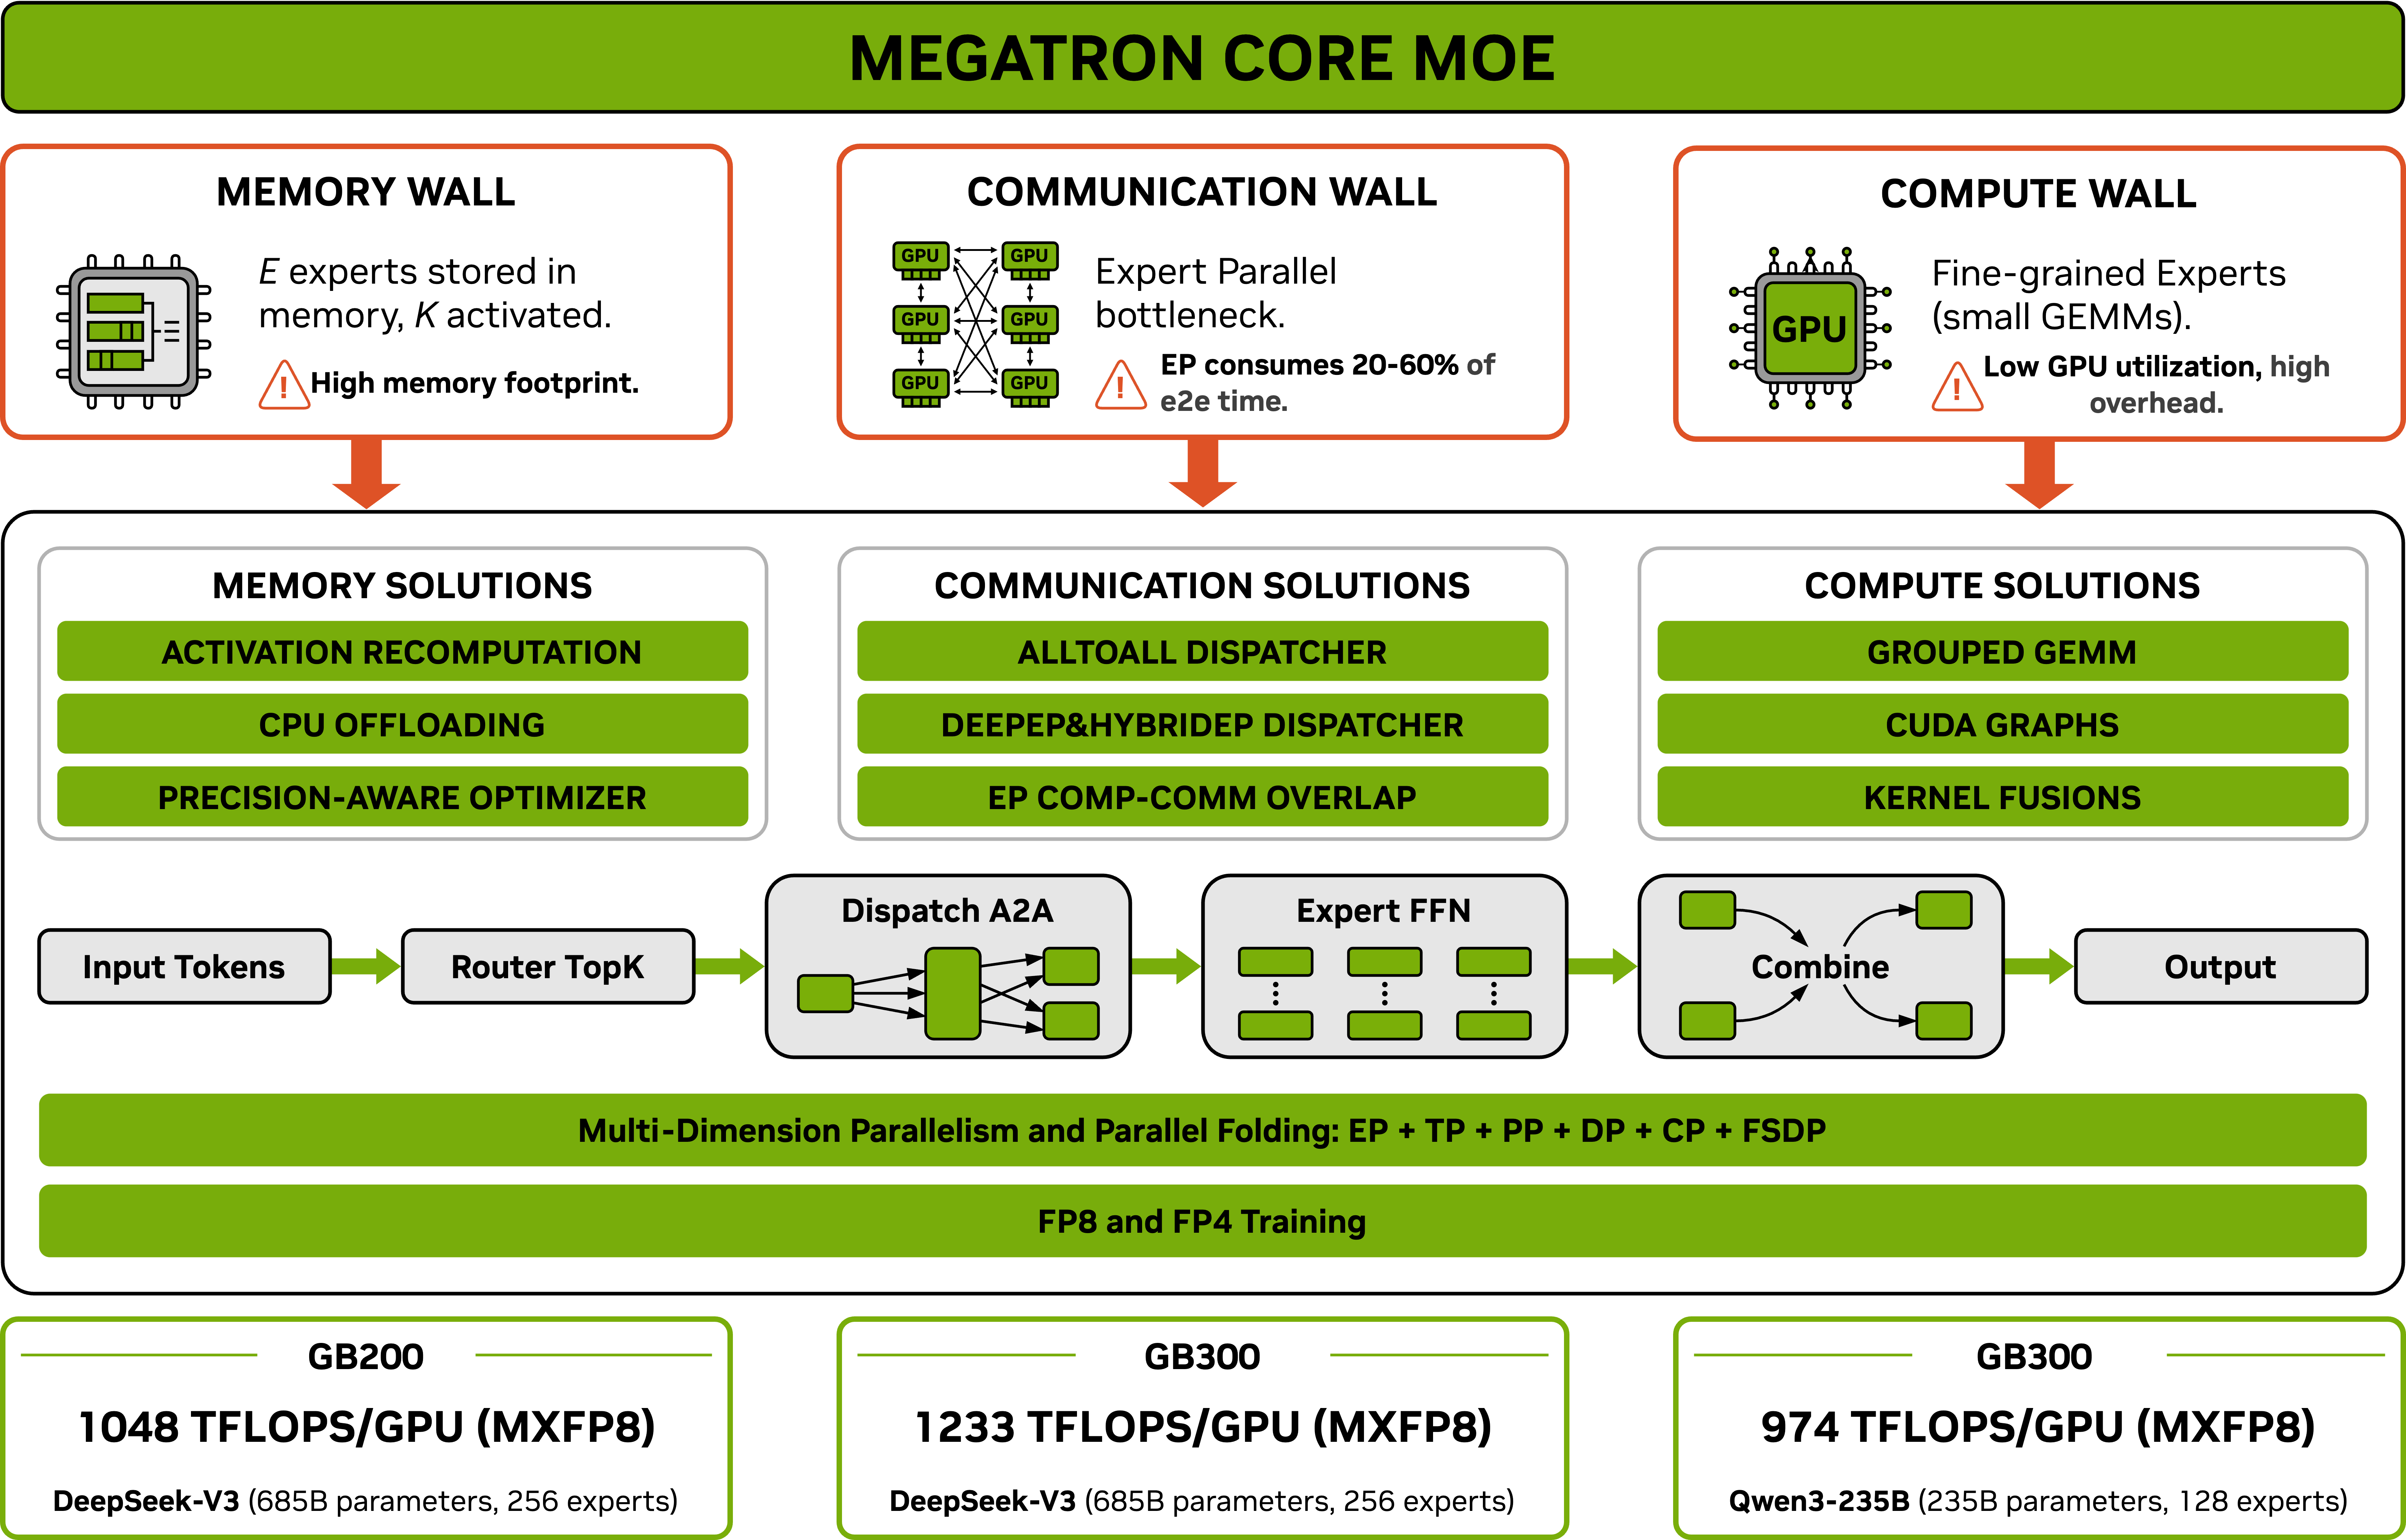
\includegraphics[width=0.93\textwidth,trim=0 0pt 0 2pt,clip]{figures/megatron_core_moe.drawio.png}
    \label{fig:graphical-abstract}
\end{figure}
\vspace{2ex}
\tableofcontents % Add a table of contents
\newpage

\section{引言}

大规模训练稠密 Transformer需要随着模型大小线性增长的计算 \cite{kaplan2020scaling,hoffmann2022chinchilla}。专家混合 (MoE) 模型遵循不同的扩展模式：通过将每个令牌路由到选定的专家网络子集而不是激活所有参数，每个令牌的计算量随模型大小呈亚线性增长 \cite{shazeer2017,fedus2022switchtransformersscalingtrillion}。最近的 MoE 模型已经证明，相对于质量匹配的密集模型，训练成本降低了几个数量级 \cite{jiang2024mixtralexperts,deepseekai2025deepseekv3technicalreport,Cai_2025}。

然而，大规模训练 MoE 会带来系统挑战，而密集模型框架并不是针对这些挑战而设计的。本报告介绍了 Megatron-Core MoE，Megatron-Core 中的 MoE 训练堆栈~\cite{shoeybi2020megatronlmtrainingmultibillionparameter}，涵盖高吞吐量训练万亿参数级 MoE 模型所需的架构、并行策略和系统优化。

\subsection{混合专家}

专家混合 (MoE) 模型通过一组称为 \emph{专家}，连同轻量级 \emph{路由器} （或门控网络）动态选择处理每个输入的专家 \cite{shazeer2017,jacobs1991adaptive,eigen2013learning}。在基于 Transformer 的语言模型的背景下 \cite{vaswani2017attention}，MoE 层通常取代密集的前馈网络 (FFN) 块：MoE 层包含多个 FFN 专家，而不是应用于所有令牌的单个 FFN，并且每个令牌都路由到一个小子集（例如，top-$k$）这些专家基于学习到的路由权重。

形式上，给定输入令牌表示 $\mathbf{x}$，路由器计算概率分布 $E$ 专家：
\[
\mathbf{p}(\mathbf{x}) = \text{Softmax}(\mathbf{W}_r \mathbf{x})
\]
然后，MoE 层的输出被计算为所选专家输出的加权组合：
\[
\text{MoE}(\mathbf{x}) = \sum_{i \in \text{TopK}(\mathbf{p}(\mathbf{x}))} p_i(\mathbf{x}) \cdot E_i(\mathbf{x})
\]
在哪里 $E_i$ 表示 $i$-th 专家网络。该架构提供了三个关键优势：通过添加更多专家，模型容量可以独立于计算成本而增长（\emph{可扩展容量}）；每个令牌仅激活一小部分参数，相对于同等大小的密集模型减少了 FLOP（\emph{计算效率}）；不同的专家可以专注于不同的输入类型（\emph{专业化}）。附录~\ref{sec:notation} 提供本报告中使用的所有符号和缩写的符号参考。

虽然这个概念可以追溯到 20 世纪 90 年代初 \cite{jacobs1991adaptive,eigen2013learning}，MoE 与现代Transformer的集成重新激发了人们的兴趣。 GShard 开创了大规模分布式 MoE 训练的先河，引入了专家并行性和负载平衡辅助损失 \cite{lepikhin2020gshard}。 Switch Transformer 证明 MoE 可以扩展到万亿参数，同时保持训练稳定性 \cite{fedus2022switchtransformersscalingtrillion}。 GLaM 表明 MoE 可以以训练成本的一小部分来匹配密集模型质量 \cite{du2022glamefficientscalinglanguage}。包括 Tutel 在内的框架 \cite{hwang2023tutel} 和 DeepSpeed-MoE \cite{rajbhandari2022deepspeedmoe} 进一步完善MoE 训练体系。

MoE在研究和行业中的采用加速了。 Mixtral-8x7B 表明开放权重 MoE 模型可以匹配专有的密集模型，同时降低推理成本 \cite{jiang2024mixtralexperts}。 DeepSeek-V2 和 DeepSeek-V3 通过细粒度专家架构对此进行了扩展，使用数百个小型专家来最大化容量计算比 \cite{dai2024deepseekmoe,deepseekai2024deepseekv2strongeconomicalefficient,deepseekai2025deepseekv3technicalreport}。 NVIDIA 的 Nemotron-3 系列~\cite{nvidia2025nemotron3} 采用混合 Mamba-Transformer MoE 架构和 LatentMoE~\cite{elango2026latentmoe}，使用 Megatron-Core 进行大规模训练。扩展定律研究证实，细粒度 MoE 实现了有利的计算优化权衡 \cite{krajewski2024scaling,ludziejewski2025jointmoescalinglaws}，加速了这一趋势——同时放大了它所带来的系统挑战。

\subsection{训练大规模 MoE 模型的挑战}\label{sec:challenges}

随着模型扩展到数百个单体容量更小的专家，MoE 训练的系统挑战也成比例增长。这些挑战源于一个根本原因：MoE \textbf{稀疏性}---表现为 \emph{参数计算不匹配} （总参数远远超过主动计算，本节）和 \emph{密集-稀疏不匹配} （注意层和 MoE 层需要冲突的并行配置，第 ~\ref{parallelism-strategies}).

\textbf{核心的不对称来自于稀疏性。} 在稠密 Transformer中，每个参数都参与每个训练步骤。一个模型与 $N_{\text{total}}$ 参数大致需要 $6 N_{\text{total}}$ 每个令牌的 FLOP 数（向前和向后组合），因此参数和每个令牌的计算规模是同步的。将模型拆分到更多 GPU 上通常也会以相同的比例拆分计算，从而使每个 GPU 保持足够的繁忙，从而保持较小的通信开销。

对于 MoE 来说，稀疏性会导致这种耦合破坏：仅 $K$ 的 $E$ 每个令牌激活的专家总数，因此每个令牌的计算量大致为 $6 N_{\text{active}}$ 而不是 $6 N_{\text{total}}$， 在哪里 $N_{\text{active}}$ 规模与 $K$ 尽管 $N_{\text{total}}$ 规模与 $E$， 和 $K \ll E$。这造成了基本的参数计算不匹配：与每个令牌的活动参数匹配的密集模型相比，MoE 模型的总参数要多得多，通常是一个数量级。 DeepSeek-V3 具体说明了这一点：总共 685B 个参数，但每个令牌只有 37B 个活跃参数，即 18 个$\times$ 差距。

由于每个标记的计算量如此之少，模型分区比密集模型需要更多的关注——天真地对专家矩阵进行分片（如张量并行）会分割已经很小的计算，从而使它们的效率更低。由于MoE专家是独立的网络，因此自然的策略是 \emph{专家并行性} (EP)：将不同的专家放在不同的 GPU 上，保留全尺寸的专家 GEMM。 EP 引入了全对全通信，以将令牌路由到其指定的 GPU（第~\ref{parallelism-strategies} 详细说明了为什么 EP 是首选以及并行折叠如何解决由此产生的挑战）。这种参数计算不匹配和 EP 的通信需求共同造成了三个紧密耦合的挑战—— \emph{三堵墙}---限制了MoE的每个训练步骤：

\textbf{内存墙。} 全部 $E$ 专家的参数、梯度和优化器状态在训练期间必须驻留在内存中，即使只是 $K$ 激活每个令牌。这产生的内存压力远远超过具有可比的每个令牌计算的密集模型的内存压力~\cite{fedus2022switchtransformersscalingtrillion,Cai_2025}。减轻这种压力需要在其他方面进行支出：在更多设备上分配参数成本 \emph{通信带宽};重新计算激活而不是存储它们的成本 \emph{额外的计算};卸载到主机内存成本 \emph{PCIe带宽}。动态路由使事情变得更加复杂：当一些专家收到不成比例的负载时，不均匀的令牌分布会导致不可预测的内存峰值~\cite{lepikhin2020gshard,wang2024auxiliarylossfreeloadbalancingstrategy}.

\textbf{通信墙。} EP要求全体集体向指定的专家发送令牌并收集结果~\cite{lepikhin2020gshard}。每个 all-to-all 中的每 GPU 发送量约为 $T \cdot K \cdot h \cdot \frac{EP-1}{EP}$， 在哪里 $T$ 是本地令牌计数， $K$ top-$k$， 和 $h$ 隐藏维度；完整的调度和组合周期使该周期加倍。随着 EP 的增长，这个数量饱和，但通信逐渐从高带宽节点内链路（例如 NVLink）转移到更窄的节点间互连，其中可用带宽下降了一个数量级~\cite{deepep2025}。同时，稀疏激活模式提供了有限的计算来与这种通信重叠。在像 DeepSeek-V3 这样的架构中，专家跨越多个节点，未优化的 all-to-all 可能会消耗多达 60\% 的总训练时间。

\textbf{计算效率墙。} MoE 引入了密集模型中不存在的计算效率低下的问题：
\begin{itemize}[nosep,leftmargin=*]
    \item \textbf{小型 GEMM。} 细粒度专家会产生许多未充分利用 GPU 计算单元的小型矩阵乘法~\cite{megablocks}。在我们的测量中，GEMM 占 $\sim$70\% Llama-3 405B（密集）的执行时间但低于 50\% 在 DeepSeek-V3 (MoE) 中。剩余部分由随张量计数而不是 FLOP 计数扩展的操作消耗。
    \item \textbf{路由和排列开销。} 密集模型中不存在的令牌路由和排列，添加 $\sim$9\% 即使在优化后也可以对执行时间进行分层。
    \item \textbf{负载不平衡。} 动态路由为专家分配的令牌数量不均匀，导致一些专家超载，而另一些则闲置，浪费计算能力~\cite{wang2024auxiliarylossfreeloadbalancingstrategy}.
    \item \textbf{主机开销。} 由于稀疏性和路由，MoE 会针对相同数量的 FLOP 启动更多内核，并且每次启动都会带来固定的主机端成本，这些成本加起来会使 GPU 在内核之间处于空闲状态。在无滴式 MoE 中，动态张量形状还需要昂贵的主机设备同步。
\end{itemize}

这三堵墙紧密相连：优化一堵墙通常会将压力转移到另一堵墙。增加批量大小可以提高 GEMM 利用率，但会增加内存压力和通信量。 CUDA Graph 消除了主机开销，但需要静态张量形状，这与无丢路由相冲突。跨专家对令牌进行分组可以提高计算效率，但会使负载平衡变得复杂。部分~\ref{parallelism-strategies} 提供 EP 和 Parallel Folding 底层的详细并行性分析；部分~\ref{key-features-optimizations} 介绍了Megatron Core的集成方法，用于解决所有三堵墙的问题，同时管理它们的相互作用。


\subsection{Megatron Core MoE}
内置于 Megatron-Core，一个基于 PyTorch 的库，用于大规模 Transformer 训练~\cite{shoeybi2020megatronlmtrainingmultibillionparameter,paszke2019pytorchimperativestylehighperformance}，这个 MoE 训练堆栈同时解决了所有三堵墙：

\textbf{多维并行性。} 专家并行 (EP) 与张量、管道、序列和数据并行集成。MoE 并行折叠 \cite{liu2025moeparallelfoldingheterogeneous} 解耦注意力和 MoE 层配置，打破传统 $\text{EP} \leq \text{DP}$ 约束，并支持针对特定模型架构和硬件拓扑定制配置。

\textbf{内存优化。} 细粒度激活重新计算、内存高效排列、精度感知优化器和激活卸载可在不牺牲吞吐量的情况下减少内存占用 \cite{korthikanti2022reducingactivationrecomputationlarge,a2023learningwithdistributedoptimization}。专家 GEMM、激活和通信中的全面降低精度训练（FP8 和 FP4）支持进一步减少激活存储，同时通过选择性精度策略保持收敛。

\textbf{通信优化。} 高性能令牌调度程序（DeepEP、HybridEP）可最大限度地提高带宽利用率。通信计算重叠隐藏了专家计算背后的所有延迟。

\textbf{计算优化。} 分组 GEMM 内核、内核融合、CUDA 图和无同步执行解决了细粒度 MoE 架构中固有的计算碎片问题。

\textbf{生产特点。} 负载平衡策略、具有容量控制的令牌丢弃、分布式优化器和 FSDP 支持、具有灵活重新分片的分布式检查点以及从密集检查点进行升级可实现大规模部署。
MoE 堆栈的模块化设计可实现快速实验，而其生产级优化则支持从研究原型到万亿参数模型的训练~\cite{nvidiamcoremoeuserguide}。本报告解释了该堆栈提供的功能、做出关键设计决策的原因以及它们如何应对 MoE 训练挑战，并提供配置和调整的实用指导。

\subsection{本文的结构}

本报告的其余部分遵循从架构到优化再到评估的进展：

\begin{itemize}

\item \textbf{部分~\ref{meg-core-architecture}：Megatron-Core MoE 架构。}
分两部分介绍Megatron-Core MoE的设计：MoE 层本身的内部设计（路由器、令牌调度程序、专家）和四阶段前向传递（路由、调度、计算、组合），然后是外部设计，包括与Transformer模型的集成、并行进程组组织和专家参数的优化器处理。

\item \textbf{部分~\ref{parallelism-strategies}：通过并行折叠和多维并行性缩放 MoE。}
研究 MoE 的稀疏性如何打破密集训练的并行性假设，为什么需要专家并行 (EP) 和传统策略，以及 MoE 并行折叠如何解决注意力层和 MoE 层之间产生的密集稀疏不匹配，从而解耦它们的并行配置，以实现万亿参数规模的灵活、高效映射。

\item \textbf{部分~\ref{key-features-optimizations}：打破内存、通信和计算效率的障碍。}
介绍了 Megatron-Core MoE 针对三个基本障碍的解决方案：内存墙（激活管理、重新计算策略、卸载、分布式参数存储）、通信墙（优化调度程序，包括 DeepEP 和 HybridEP、通信计算重叠）和计算效率墙（分组 GEMM、内核融合、CUDA 图形、无滴 MoE 的无同步执行）。

\item \textbf{部分~\ref{sec:reduced-precision-training}：MoE 的 FP8/FP4 低精度训练。}
涵盖降低精度训练作为横切优化，通过减少激活内存、减半通信量和加速 Tensor Core GEMM，同时影响所有三堵墙，同时提出选择性精度策略以保持训练稳定性。

\item \textbf{部分~\ref{sec:long-context-training}：长情境MoE 训练。}
检查长上下文场景（16K 到 64K+ 令牌）如何从根本上改变注意力计算占主导地位的优化格局，并提出通过上下文并行和张量并行缩放来管理激活内存增长的技术。

\item \textbf{部分~\ref{sec:production-features}：生产特点。}
描述生产训练的操作功能：用于稳定训练的负载平衡和令牌丢弃、用于与并行性无关的重新分片的分布式检查点、从密集检查点升级以及与多令牌预测集成。

\item \textbf{部分~\ref{performance-evaluations}：绩效评估。}
通过跨 GB200 和 H100 平台的 DeepSeek-V3 和 Qwen3-235B 的实证基准验证框架的有效性，展示完整优化堆栈的影响。

\item \textbf{部分~\ref{sec:best-practices}：DeepSeek-V3 案例研究的性能最佳实践。}
提供用于识别最佳并行配置的系统工作流程，并通过详细的 DeepSeek-V3 案例研究进行验证，该案例研究演示了优化如何协同工作以实现最先进的性能。

\item \textbf{部分~\ref{sec:rl}：强化学习中的Megatron Core MoE。}
解决新兴的 RL 训练后范式，涵盖 RL 工作负载特有的挑战（可变序列长度、内存卸载、在线权重导出）、Megatron-Bridge 与流行的 RL 框架的集成，以及 RL 特定的优化，包括打包序列支持、动态上下文并行性和路由器重放。

\end{itemize}


\section{Megatron Core MoE 架构}\label{meg-core-architecture}

本节分两部分介绍 Megatron-Core 的 MoE 实现架构。我们首先描述 \textbf{内部设计} MoE 层本身：其模块化组件（路由器、令牌调度程序、专家）以及将输入令牌转换为输出表示的四阶段前向传递。然后我们检查 \textbf{外部设计}：如何组织并行进程组以支持分布式执行，以及优化器如何以不同于密集层的方式处理专家参数。

\subsection{MoE 层架构和前向传递}\label{sec:moe-layer-architecture}

MoE 层用一组专家 FFN 取代了Transformer块中的密集前馈网络 (FFN)，只有其中的一个子集处理每个令牌。 Megatron-Core 通过三个模块化组件（一个 \emph{路由器} 对于令牌到专家的分配， \emph{令牌调度程序} 用于跨 GPU 通信，以及 \emph{专家} 用于计算）通过四级前向传递连接，如图所示 \figref{fig:moe-forward-pass}。这种关注点分离可以实现独立优化：路由器可以融合到 CUDA Graph 中，而不影响调度程序逻辑，调度程序可以在 all-to-all 和 DeepEP 之间交换，而无需修改专家计算，专家实现可以透明地使用不同的 GEMM 后端。

\subsubsection{前向传递：路由、调度、计算、组合}

MoE 层通过四个连续阶段处理输入令牌：

% Fix the typo in this figure
\begin{figure}[ht]
\centering
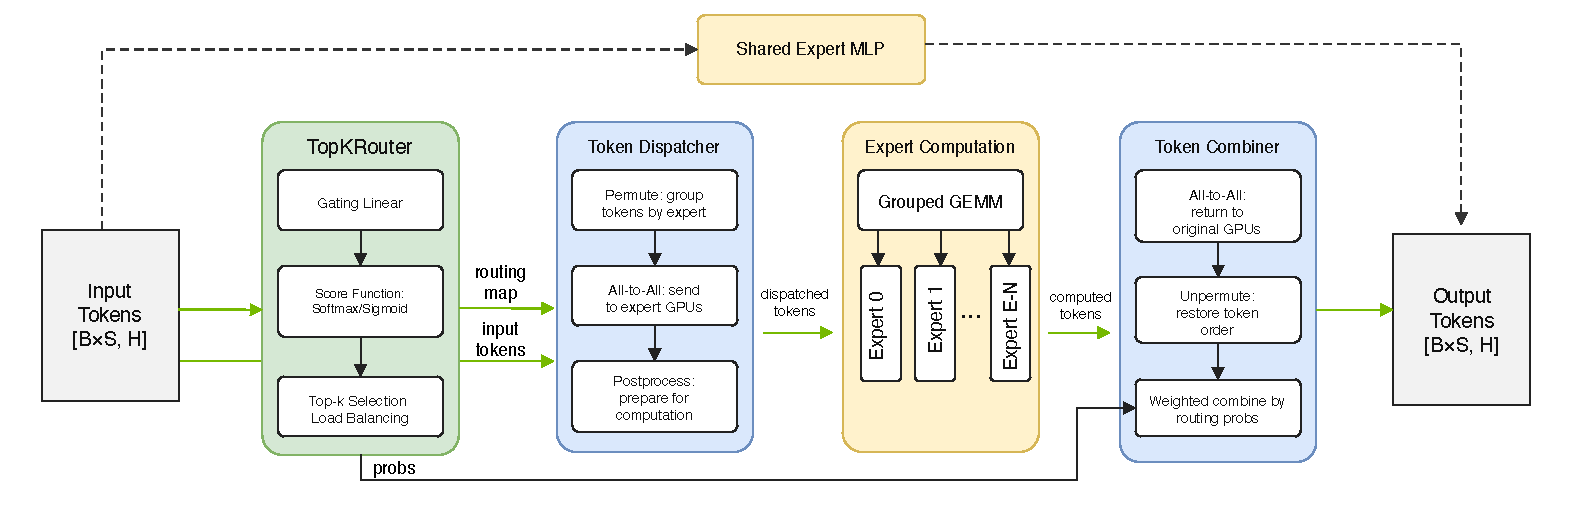
\includegraphics[width=0.9\textwidth]{figures/moe_forward_pass.drawio.pdf} 
\caption{数据流经 MoE 层：路由、调度、计算和组合阶段。}
\label{fig:moe-forward-pass}
\end{figure}

\textbf{第一阶段：路线。} 这 \texttt{TopKRouter} 确定哪些专家处理每个令牌。学习的线性投影将每个标记的隐藏状态映射到 $E$ logits（每个专家一个），评分函数（softmax 或 sigmoid）将 logits 转换为概率，并且 top-$k$ 选择确定每个令牌得分最高的专家。路由器输出两个张量： \texttt{probs} 包含路由权重，以及 \texttt{routing\_map}，一个布尔掩码，指示令牌专家分配。为了获得许多专家的数值稳定性，路由器可以通过以下方式在 FP32 中运行 \texttt{-{}-moe-router-dtype fp32}.

\textbf{第二阶段：调度。} 令牌调度程序为跨 GPU 通信准备令牌。它首先对令牌进行排列，以便发往同一专家的所有令牌都是连续的；这种排列对于专家方面的高效密集 GEMM 至关重要。然后，调度程序使用三个后端之一将令牌转移到托管其指定专家的 GPU：AllGather（简单但内存密集型）、all-to-all（基于标准 NCCL）或 Flex（支持 DeepEP 和 HybridEP 等优化后端）。

\textbf{第三阶段：专家计算。} 每个 GPU 对收到的令牌执行其本地专家。所有本地专家通过以下方式在单个分组 GEMM 调用中运行 \texttt{TEGroupedMLP}，即使单个专家工作负载很小，也能最大限度地提高 GPU 利用率。

\textbf{第四阶段：合并。} 反向通信将处理后的令牌返回到其原始 GPU，然后进行取消排列以恢复原始序列顺序。如果配置了共享专家，则在此阶段添加其输出（可以选择与路由专家并行计算）。

\subsubsection{路由器：令牌到专家的分配}

路由器通过两个操作将全局令牌批次转换为专家特定的工作负载 \cite{shazeer2017}:

\begin{enumerate}
    \item \textbf{门控：} 线性投影 $\mathbf{W}_r \in \mathbb{R}^{h \times E}$ 映射每个标记的隐藏状态 $\mathbf{x} \in \mathbb{R}^h$ 到逻辑 $\mathbf{l} = \mathbf{W}_r^\top \mathbf{x} \in \mathbb{R}^E$.

    \item \textbf{top-$k$ 选择：} 评分函数将 logits 转换为概率：softmax ($p_i = e^{l_i} / \sum_j e^{l_j}$) 或sigmoid ($p_i = \sigma(l_i) / \sum_j \sigma(l_j)$，由 DeepSeek-V3 使用 \cite{deepseekai2025deepseekv3technicalreport}）。top-$k$ 每个令牌都会选择概率最高的专家。
\end{enumerate}

\begin{figure}[ht]
    \centering
    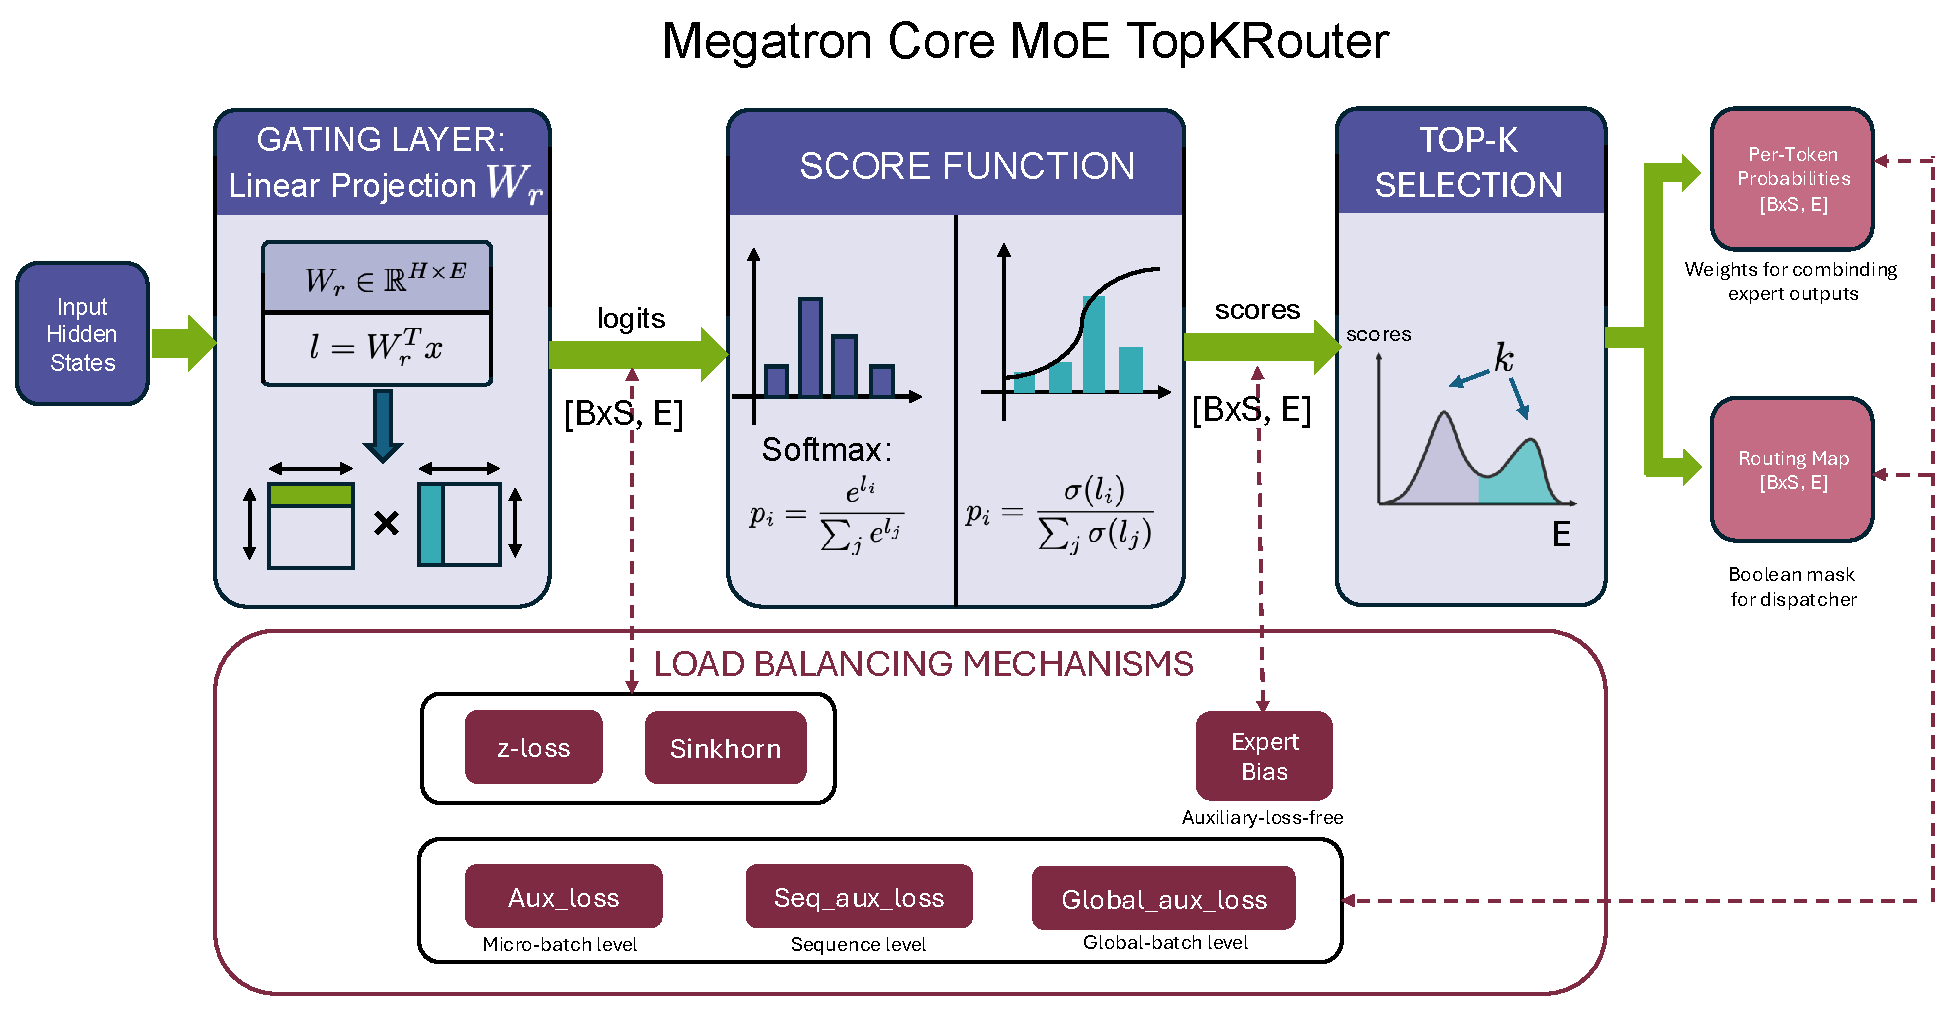
\includegraphics[width=0.85\textwidth]{figures/router.pdf}
    \caption{路由器架构：线性投影、分数函数、top-$k$ 选择和负载平衡。}
    \label{fig:router-architecture}
\end{figure}

专家利用率不均匀会降低训练效率和模型质量。如图所示 \figref{fig:router-architecture}，Megatron-Core支持多种负载均衡策略；这些都在章节中讨论~\ref{sec:production-features}.

\subsubsection{令牌调度程序：通信抽象}

调度程序通过六阶段管道管理 GPU 之间的令牌移动： \texttt{dispatch\_preprocess} $\rightarrow$ \texttt{token\_dispatch} $\rightarrow$ \texttt{dispatch\_postprocess} （向前），以及 \texttt{combine\_preprocess} $\rightarrow$ \texttt{token\_combine} $\rightarrow$ \texttt{combine\_postprocess} （落后）。

\textbf{通信后端。} 可以使用三种调度程序类型：
\begin{itemize}
    \item \textbf{齐聚} (\texttt{allgather})：每个 GPU 收集本地专家的所有标记和过滤器。简单但占用内存；适用于小 EP 尺寸。
    \item \textbf{多对多} (\texttt{all-to-all})：基于标准 NCCL 的点对点通信 \cite{lepikhin2020gshard}。每个 GPU 仅发送每个目的地所需的令牌。可扩展性良好，但会产生同步开销。
    \item \textbf{柔性} (\texttt{flex}）：支持DeepEP的统一设计（仅集成高吞吐量内核，通过重叠隐藏NVLink通信延迟） \cite{deepep2025} 和 HybridEP（高带宽 MoE 通信内核，可在 NVL72 等富含 NVLink 的拓扑上提供更好的性能）。
\end{itemize}

\subsubsection{专家：计算模块}

每个专家都是一个带有可选门控的两层 MLP（用于 SwiGLU/GeGLU 激活） \cite{shazeer2020glu}）。分组 GEMM 可实现多个专家计算的高效批处理 \cite{megablocks,hwang2023tutel}。有两种实现方式可供选择：

\begin{itemize}
    \item \textbf{TE集团MLP}: Transformer发动机 \cite{nvidia_transformer_engine} 支持 FP8 和 FP4 量化的优化实现。
    \item \textbf{顺序MLP}：循环中一次执行一个专家。对于调试很有用，但速度明显慢。
\end{itemize}

\textbf{共享专家。} 一些架构（DeepSeek-V2/V3 \cite{deepseekai2024deepseekv2strongeconomicalefficient,deepseekai2025deepseekv3technicalreport}, 琪文 \cite{qwen2025qwen25technicalreport}）包括一个共享专家，无论路由如何，它都会处理所有令牌。共享专家计算可以与调度-计算-组合管道并行运行，隐藏其延迟。见章节~\ref{sec:production-features} 了解详情。


\subsection{系统集成：并行性和优化器}\label{sec:moe-system-integration}

描述了 MoE 层的内部工作原理后，我们现在研究它如何集成到分布式训练系统中：并行进程组和优化器处理。

\subsubsection{平行集团管理}

MoE 层需要与密集层不同的进程组，因为不同的组件具有不同的通信模式。Megatron Core通过以下方式组织这些团体 \texttt{ProcessGroupCollection}:

\begin{lstlisting}
ProcessGroupCollection
|-- Attention Layer Groups: tp, cp, dp, pp
|-- Expert Layer Groups:    ep, expt_tp, expt_dp, pp
\end{lstlisting}

每个 MoE 组件根据其通信要求使用特定的组：

\begin{table}[ht]
\centering
\begin{tabular}{lll}
\toprule
\textbf{成分} & \textbf{使用的组} & \textbf{原因} \\
\midrule
路由器 & \texttt{tp}, \texttt{cp}, \texttt{tp\_cp} & EP 排名中的权重重复 \\
令牌调度程序 & \texttt{ep}, \texttt{tp\_ep} & 跨专家队伍的全方位 \\
专家 & \texttt{ep}, \texttt{expt\_tp}, \texttt{expt\_dp} & 跨 EP 分片； EDP​​ 梯度降低 \\
共享专家 & \texttt{tp} & 与密集 MLP 相同 \\
\bottomrule
\end{tabular}
\caption{MoE 组件处理组映射。}
\label{tab:moe-process-groups}
\end{table}

这种分离使得 \textbf{并行折叠} （节~\ref{sec:parallel-folding})：注意力层和 MoE 层可以使用不同的 TP/DP 配置。例如，注意力层可能使用 TP=4，而 MoE 层使用具有更高 EP 的 ETP=1，独立优化每个层类型。

\subsubsection{优化器和梯度处理}

专家参数需要在分布式优化中进行独特的处理。Megatron Core使用 \texttt{Chained\-Optimizer} 它包装了针对密集参数和专家参数的单独优化器。三个关键设计决策支持正确的 MoE 优化：

\begin{enumerate}
    \item \textbf{参数识别。} 专家参数标记为 \texttt{allreduce=False}，将它们与使用标准数据并行梯度下降的密集参数区分开来。

    \item \textbf{单独的还原组。} 密集层减少了梯度 \texttt{dp\_cp\_group} （完全数据并行），而专家则减少跨 \texttt{expt\_dp\_group} （专家数据并行性）。这确保了梯度在正确数量的副本上平均。

    \item \textbf{梯度缩放。} 专家梯度的缩放比例为 \texttt{edp\_size / dp\_size} 考虑专家（处理依赖于路由的令牌子集）与密集层所看到的不同有效批量大小。
\end{enumerate}

这种设计允许 ZeRO 式优化器状态分片 \cite{rajbhandari2020zero} 与 MoE 无缝协作：专家参数的优化器状态在 EP 组中进行分片，而密集参数的状态则遵循标准 DP 分片。

架构建立完毕，Section~\ref{parallelism-strategies} 解决如何跨设备分发它，以及部分~\ref{key-features-optimizations} 解决大规模出现的内存、通信和计算效率挑战。

\section{Scaling MoE：并行折叠和多维并行}\label{parallelism-strategies}

部分~\ref{sec:challenges} 确定 MoE 的稀疏性将模型大小与每个令牌计算解耦，从而产生参数计算不匹配，使得专家并行 (EP) 成为必要，但引入了全对全通信。本节将研究这种不匹配如何具体影响并行性设计。我们首先回顾密集模型的并行性基线及其所需的权衡，然后展示 MoE 的稀疏性如何打破这些策略背后的假设。最后，我们呈现 \textbf{MoE 并行折叠}，即 Megatron Core 针对 \emph{稠密-稀疏失配} 的解决方案：注意力层和 MoE 层具有相互冲突的最佳并行配置，而并行折叠解耦了它们的映射，以便每个层都可以使用其最佳拓扑。

%==============================================================================
% 3.1 Opening: Why Parallelism, and Why MoE is Different
%==============================================================================
\subsection{为什么并行，为什么 MoE 不同}\label{sec:why-parallelism}

在研究 MoE 特定的挑战之前，我们先确定并行性对于大型模型训练是必要的根本原因以及它带来的权衡。

\subsubsection{为什么大型模型训练需要并行性}

\textbf{记忆是根本的限制。} 单个 GPU 的内存有限，但训练大型模型需要同时存储模型参数、优化器状态、梯度和激活 \cite{rasley2020deepspeed}。考虑 Llama-405B \cite{grattafiori2024llama3herdmodels,touvron2023llama,touvron2023llama2} 使用 BF16 精度和 Adam 优化器进行训练：

\begin{center}
\begin{tabular}{lr}
\toprule
\textbf{成分} & \textbf{内存（Llama-405B、BF16）} \\
\midrule
型号参数 & $\sim$810GB \\
优化器状态 (Adam) & $\sim$4860GB \\
渐变 & $\sim$1620GB \\
激活（8K 序列） & $\sim$5575GB \\
\midrule
\textbf{全部的} & \textbf{$\sim$12865GB} \\
\bottomrule
\end{tabular}
\end{center}

这远远超过了任何单个 GPU 的容量。多个 GPU 不是可选的；他们是 \emph{必需的} 保持模型。

\textbf{计算吞吐量是效率的原因。} 除了内存之外，单个 GPU 的计算能力也有限。大型模型训练需要天文数字的 FLOPs；聚合多个 GPU 可以提高吞吐量，并将挂钟训练时间从几年缩短到几周。

\subsubsection{并行性的权衡}

并行性不是免费的。每个并行策略都会带来开销：

\begin{itemize}
    \item \textbf{通信开销}：GPU 之间的数据交换会消耗时间和带宽。
    \item \textbf{同步}：快速 GPU 必须在同步点等待慢速 GPU。
    \item \textbf{管道气泡}：管道并行性在管道边界引入了空闲时间。
    \item \textbf{降低计算强度}：分片会减少每个 GPU 矩阵的大小，从而降低 GEMM 效率。
\end{itemize}

结果：模型 FLOP 利用率（MFU）很大程度上受并行策略的影响，有效的并行设计可以最小化理想 MFU 与实际 MFU 之间的差距。

\textbf{密集模型的关键见解}：并行性的“成本”和“收益”成比例。更多参数需要更多 GPU，但更多参数也意味着每次前向-后向传递需要更多计算。由于计算量随着模型规模的增长而增长，因此通信在每个步骤中所占的份额较小，从而随着模型规模的扩大，保持 MFU 相对稳定。

MoE的稀疏性破坏了这种平衡。因为只有 $K$ 的 $E$ 专家激活每个令牌，总参数按比例缩放 $E$ 而每个令牌的计算规模只能与 $K$。内存需要更多 GPU，但每个令牌的计算量无法匹配，从而导致通信开销暴露。以下部分将研究这种不对称性如何打破传统并行策略的假设，以及为什么需要新的并行维度。

%==============================================================================
% 3.2 The Challenge of MoE Parallelism
%==============================================================================
\subsection{MoE 并行性的挑战}\label{sec:moe-parallelism-challenge}

传统的并行策略是为密集的 Transformer 设计的。 MoE 模型具有根本不同的计算模式，需要新的并行维度、专家并行 (EP)，并且在将 EP 与现有策略相结合时会带来独特的挑战。

\subsubsection{MoE 的并行悖论}\label{sec:parallelism-paradox}

\begin{figure}[t]
    \centering
    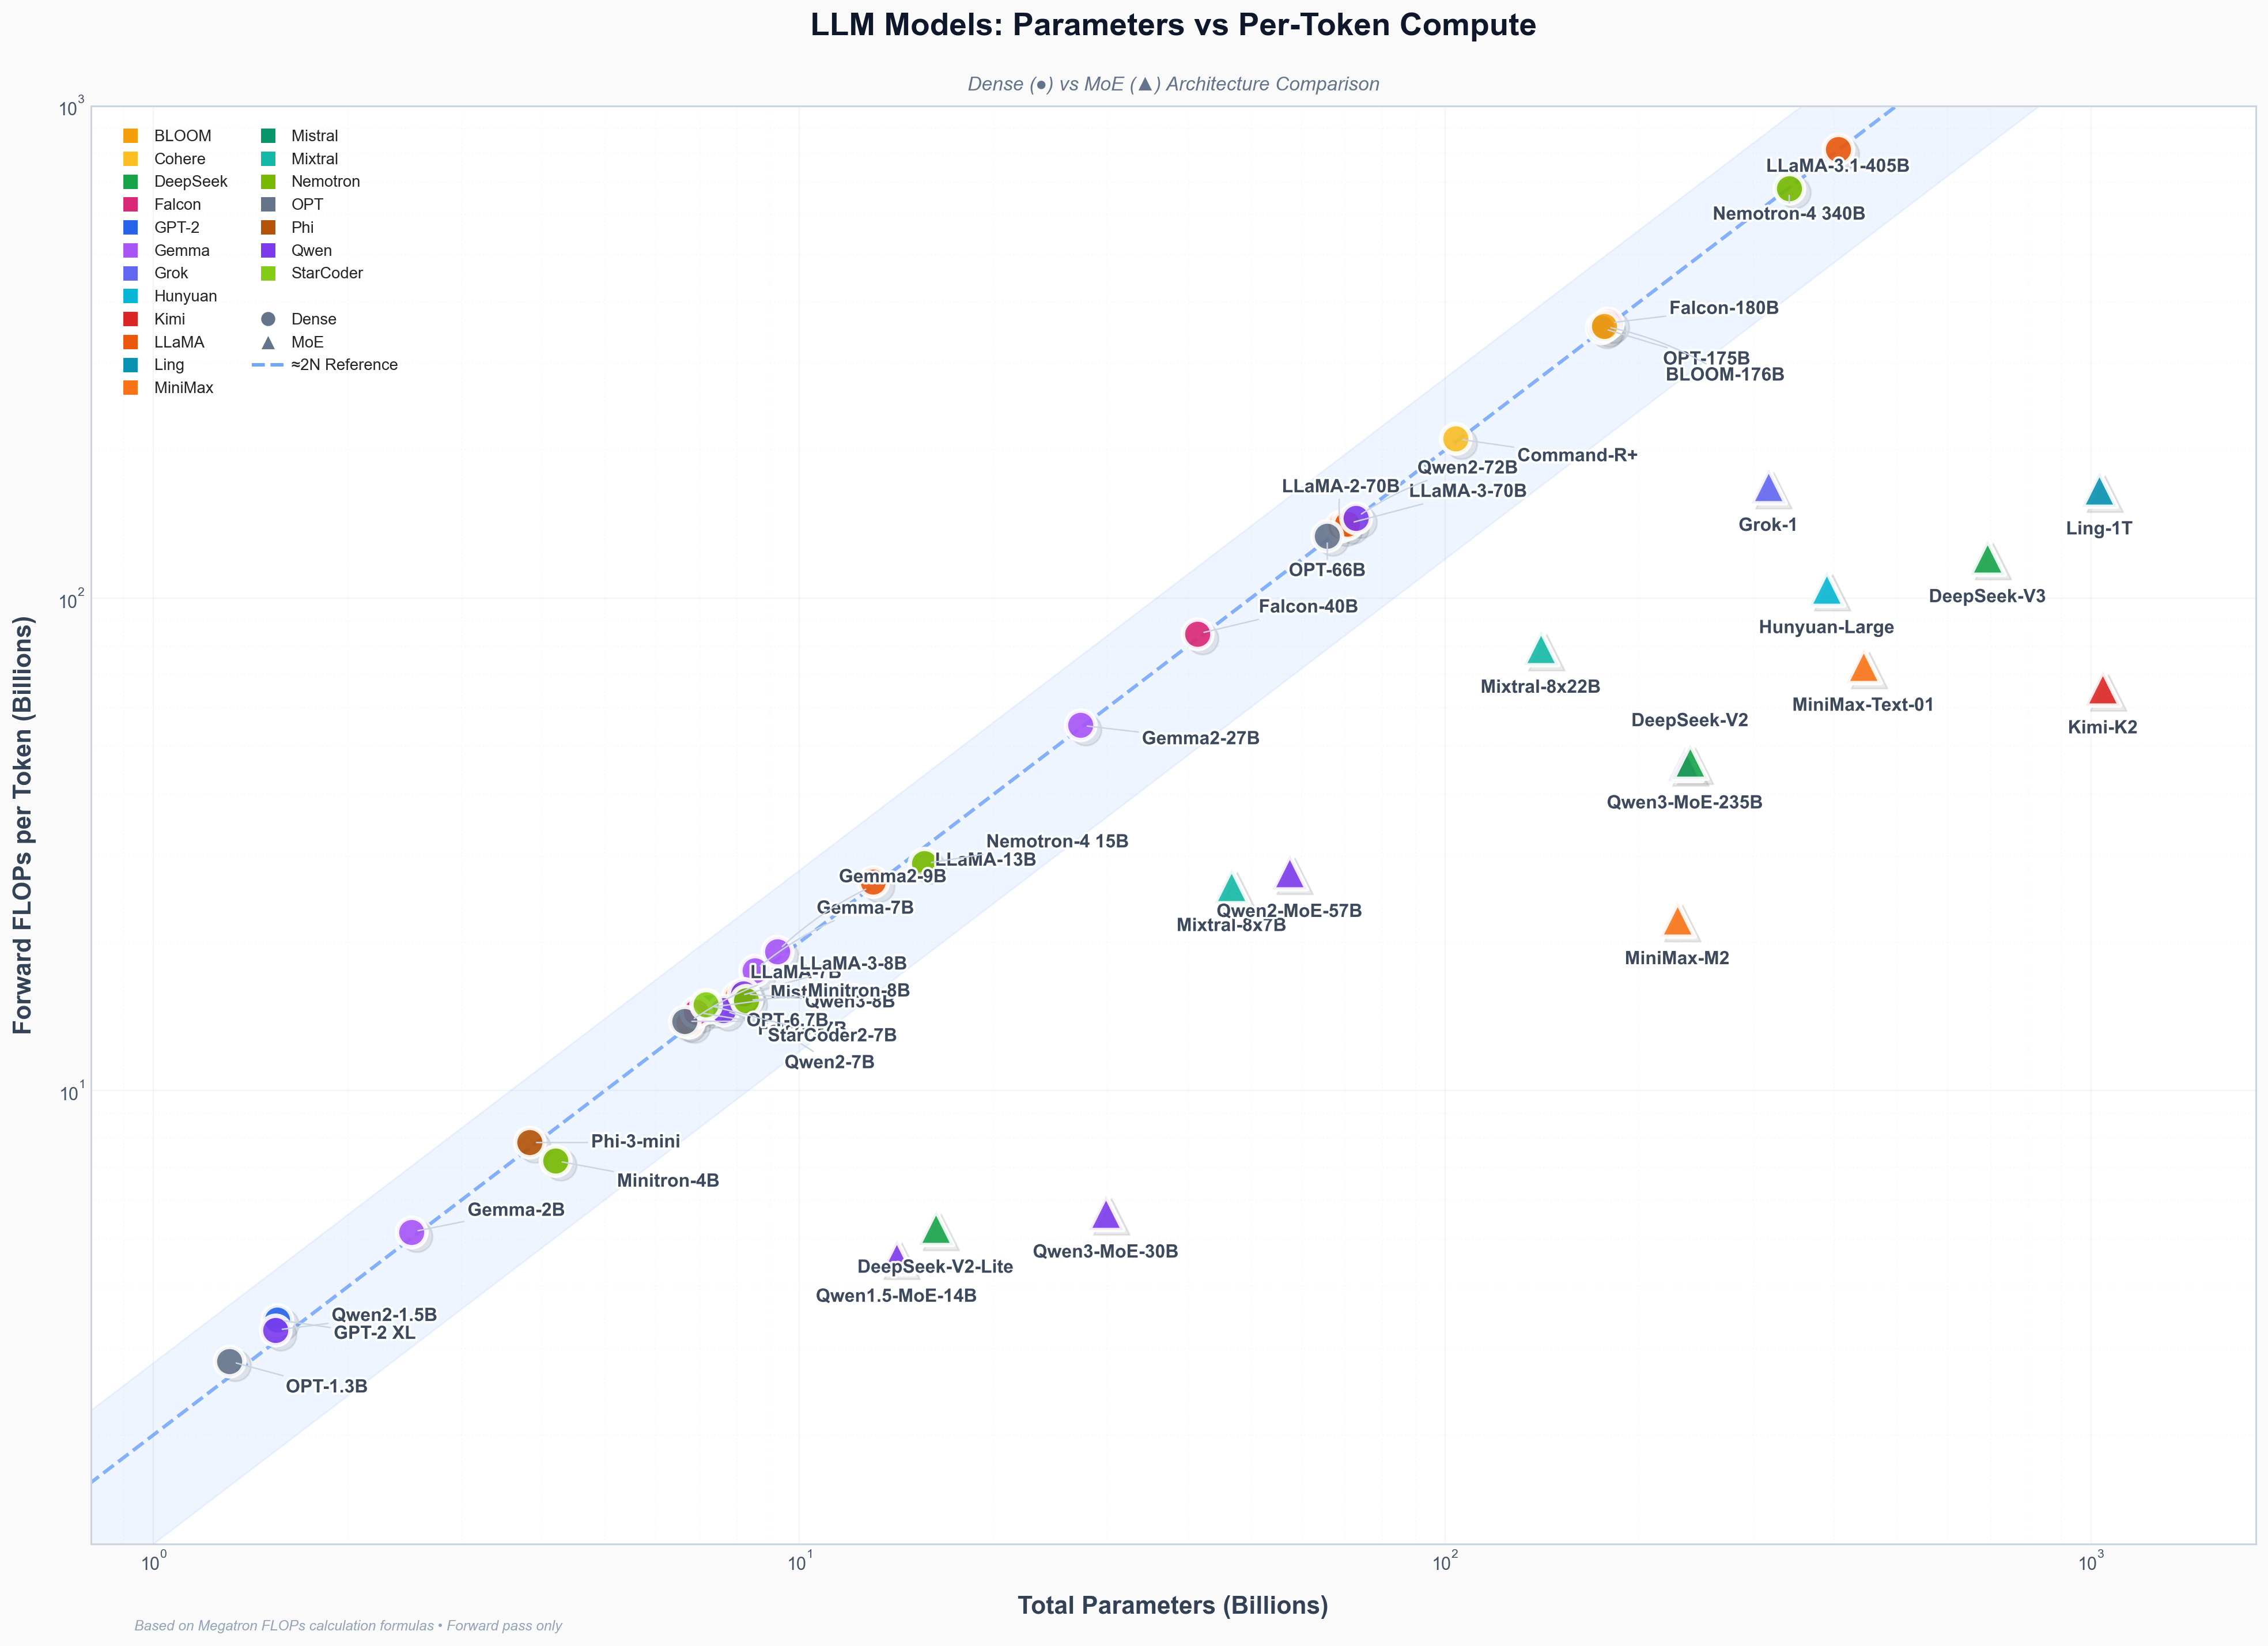
\includegraphics[width=0.95\textwidth]{figures/llm_comparison.png}
    \caption{密集模型与 MoE 模型参数/计算缩放。}
    \label{fig:parallelism-paradox}
\end{figure}

\Figref{fig:parallelism-paradox} 通过绘制总参数与 \emph{向前} 主要法学硕士的每个令牌的失败次数。密集模型（圆圈）遵循 $\approx$2N 参考线，展示 \emph{良性循环} 随着规模的扩大：增加参数需要更多的 GPU 来存储内存，但更多的参数也意味着每个令牌的计算量更大。由于计算量随着模型大小的增加而增长，因此通信在每个步骤中所占的份额较小，从而保持 MFU 稳定。

MoE 模型（三角形）打破了这个循环。它们明显低于 2N 线，以每个令牌更少的 FLOP 实现同等的功能。考虑基本的不对称性：

\begin{center}
\begin{tabular}{lccc}
\toprule
\textbf{模型} & \textbf{总参数} & \textbf{活动参数} & \textbf{比率} \\
\midrule
Llama-70B（密集） & 70B & 70B & 1:1 \\
DeepSeek-V3（MoE） & 685B & 37B & \textbf{18:1} \\
\bottomrule
\end{tabular}
\end{center}

{\footnotesize \textbf{笔记：} DeepSeek-V3 包含 671B 主模型权重和 14B 多令牌预测 (MTP) 模块权重（总共 685B）。该表显示了包括 MTP 在内的总模型参数。}

DeepSeek-V3有18个$\times$ 比其主动计算建议的参数更多，可见于 \Figref{fig:parallelism-paradox} 作为 DeepSeek-V3 位置与等效参数密集模型所在位置之间的差距。这创建了一个 \emph{复合效应}:

\begin{enumerate}
    \item \textbf{内存增长很快}，强制分布在多个 GPU 上：全部 $E$ 专家的参数、梯度和优化器状态必须驻留在内存中，并且更大的top-$k$ 通过令牌复制进一步增加激活内存。
    \item \textbf{更多通信}：通过 EP 分配专家引入了全对全流量，其流量随 $K$ （每个令牌被发送到 $K$ EP 级别的专家）。
    \item \textbf{但计算量仍然很低}：每个令牌的 FLOP 数仅可扩展 $N_{\text{active}}$ ($\propto K$）， 不是 $N_{\text{total}}$ ($\propto E$），导致计算量不足以与不断增长的通信重叠。
\end{enumerate}

结果： \textbf{MoE 训练从根本上讲是与通信相关的} 除非并行性是专门针对这种不对称性而设计的。这不是程度的问题，而是程度的问题。这是一个 \emph{质的差异} 来自密集模型。

\subsubsection{传统并行策略}\label{sec:traditional-parallelism}

Dense Transformer 训练通常结合四种并行策略：

\textbf{张量并行度 (TP)} 沿隐藏维度跨 GPU 分片权重矩阵 \cite{shoeybi2020megatronlmtrainingmultibillionparameter}。每个GPU 计算部分结果，然后AllGather 或ReduceScatter 集体组合结果。当矩阵大到足以抵消通信开销时，TP 效果很好。

\textbf{管道并行度 (PP)} 在 GPU 上按层分割模型 \cite{huang2019gpipe,narayanan2019pipedream,shoeybi2020megatronlmtrainingmultibillionparameter,qi2023zerobubblepipelineparallelism,qi2024pipelineparallelismcontrollablememory,zhang2022chimera,guan2025pipeoptimensuringeffective1f1b}。微批次流经管道，阶段之间进行点对点通信。 PP 引入了管道气泡（边界处的空闲时间）和 P2P 通信开销，但跨节点的扩展性比 TP 更好。

\textbf{数据并行性 (DP)} 跨 GPU 复制模型，每个 GPU 处理不同的数据批次 \cite{shallue2019measuringeffectsdataparallelism,bai2022moderndistributeddataparallellargescale}。梯度通过 AllReduce 同步。 DP 很简单，但需要每个 GPU 保存完整的模型。

\textbf{上下文并行性 (CP)} \cite{korthikanti2023sequence,liu2023ringattention,jacobs2023deepspeedulysses} 沿序列维度跨 GPU 划分输入序列。每个 GPU 处理序列的连续块，仅在注意力计算时需要通信，其中令牌必须跨越块边界。 CP 对于长上下文训练至关重要，其中激活记忆与序列长度呈二次方缩放。

\textbf{为什么传统的并行性对于 MoE 来说失败了：}

\begin{itemize}
    \item \textbf{MoE专家的 TP}：专家隐藏尺寸小；应用 TP 会创建更小的分片，降低计算效率，同时增加通信在总时间中所占的份额。高TP可以有效分配注意力，但是 \emph{伤害} MoE。
    \item \textbf{PP与众多专家}：MoE 模型具有大量参数，如果单独使用 PP，则需要许多管道阶段。这会产生过多的管道气泡并降低吞吐量。
    \item \textbf{单独DP}：DP 在每个 GPU 上复制完整模型。对于万亿参数模型来说，这是不可能的，因为DP不能划分参数，只能划分数据。
\end{itemize}

\subsubsection{专家并行性：第五维度}\label{sec:expert-parallelism}

传统并行分区 \emph{层数} （PP）， \emph{权重矩阵} （TP）， \emph{顺序} （CP），或 \emph{数据} （DP）。但MoE有一个独特的结构： \textbf{专家是独立的子网络}。这实现了第五个并行维度，用于分区 \emph{专家本身} 跨 GPU。

\textbf{专家并行 (EP)} 跨 GPU 分配专家 \cite{lepikhin2020gshard}。 EP 度等于 $E$，每个GPU持有 $E/\text{EP}$ 专家。前向传播过程如下：

\begin{enumerate}
    \item \textbf{路线}：路由器选择top-$k$ 每个令牌的专家。
    \item \textbf{派遣}：所有对所有的通信将令牌发送到持有其指定专家的 GPU。
    \item \textbf{计算}：每个 GPU 仅使用其本地专家来处理令牌。
    \item \textbf{结合}：所有对所有通信将结果返回到原始 GPU。
\end{enumerate}

\textbf{EP 独特的权衡}:
\begin{itemize}
    \item \textbf{通信}: 全体集体。交易量与令牌数量有关，而不是与专家数量有关。
    \item \textbf{计算}：每个 GPU 运行较少的专家，但每个专家处理其 \emph{满的} 隐藏维度。
    \item \textbf{记忆}：更高的 EP = 每个 GPU 更少的专家 = 更低的内存压力。
\end{itemize}

EP 提供两个主要优势（\figref{fig:expert-parallelism-overview}）。首先，将来自不同 GPU 的令牌分组到单个专家会增加计算强度，从而提高 GEMM 效率。其次，随着专家数量的增加，所有人对所有人的通信量保持不变；仅 GPU 数量发生变化。

\begin{figure}[ht]
    \centering
    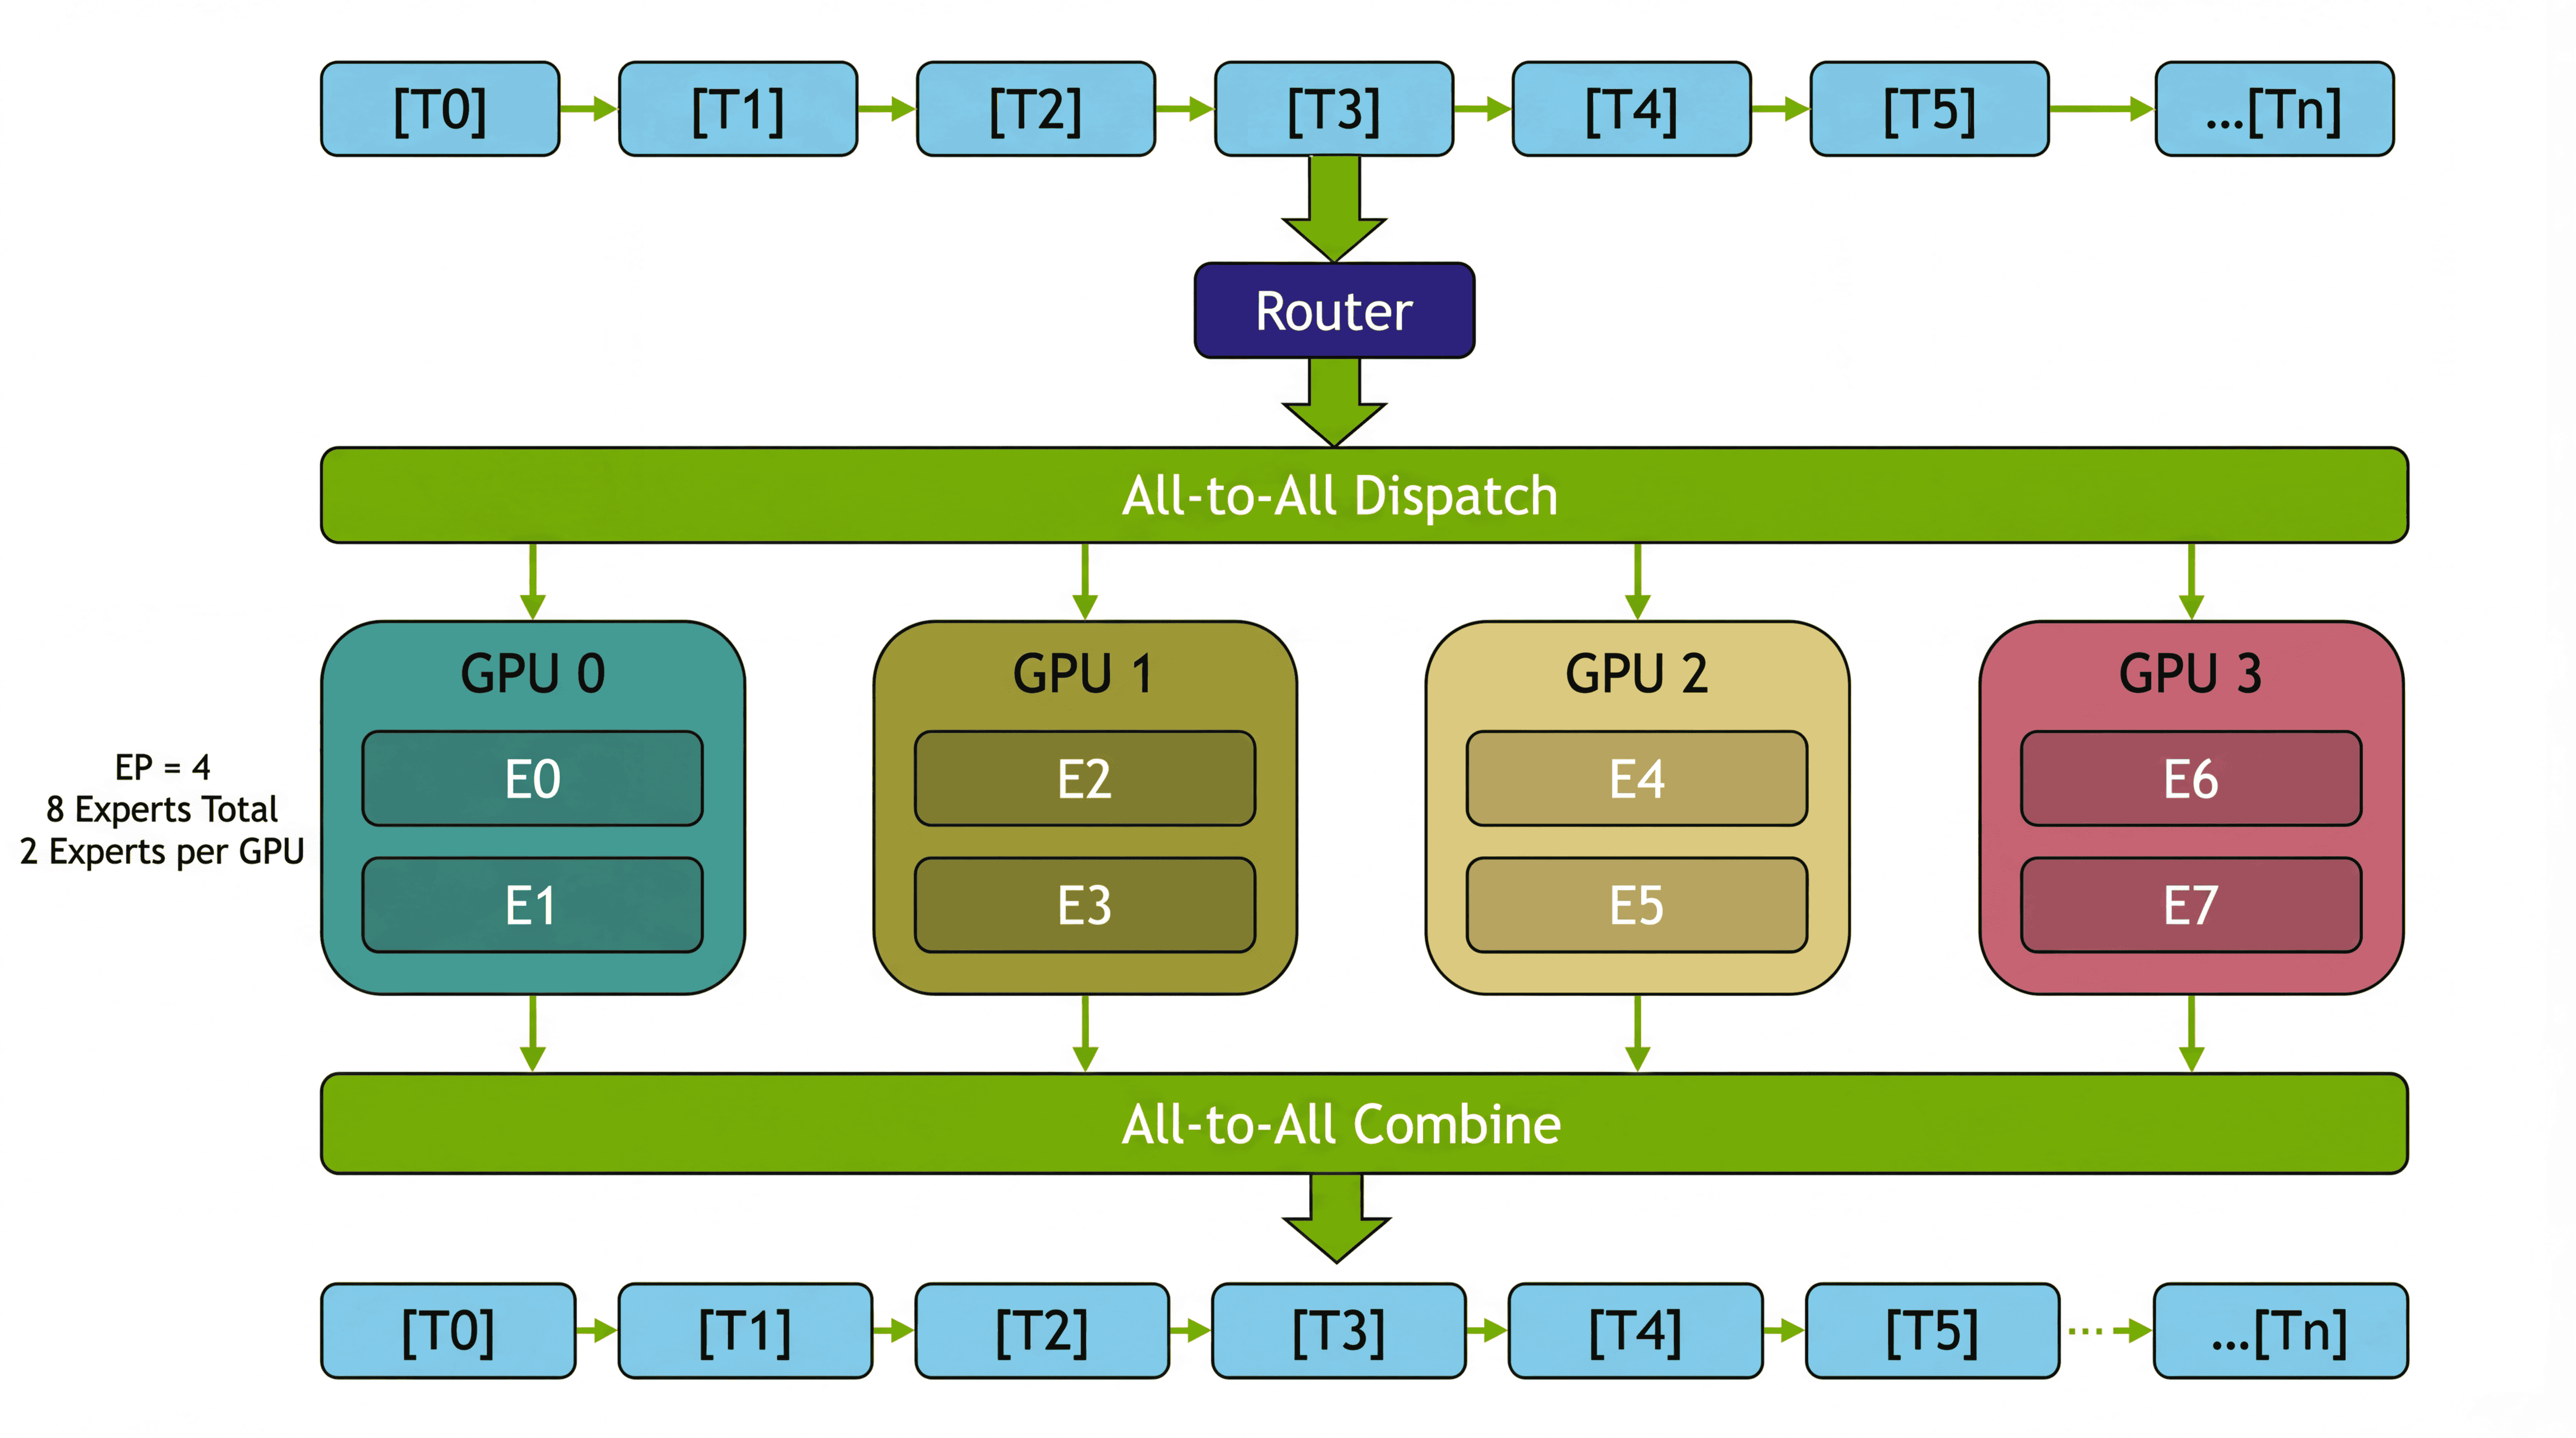
\includegraphics[width=0.9\textwidth]{figures/plots/expert_parallelism_overview_draft.png}
    \caption{专家并行 (EP) 将专家分布在 GPU 上。全面通信将令牌发送给指定的专家并合并结果。}
    \label{fig:expert-parallelism-overview}
\end{figure}

\textbf{但仅 EP 还不够。} EP仅适用于MoE 层；注意力层没有专家，仍然需要 TP、CP 或其他策略。此外，这两种层类型都需要 Pipeline Parallelism 来进一步划分模型参数以进行大规模 MoE 训练。这种异质性造成了接下来讨论的密集稀疏不匹配。

\subsubsection{EP 与传统并行性相结合的挑战}\label{sec:combining-parallelism}

单个 Transformer 块包含 \textbf{两种根本不同的计算模式} \cite{Singh_2023}，总结如表~\ref{tab:dense-sparse-comparison}:

\begin{table}[ht]
\centering
\caption{对比单个 Transformer 块内注意力层和 MoE 层的并行性要求。}
\label{tab:dense-sparse-comparison}
\begin{tabular}{lp{0.4\textwidth}p{0.4\textwidth}}
\toprule
\textbf{方面} & \textbf{注意（密集）} & \textbf{MoE（稀疏）} \\
\midrule
计算 & 每个令牌都关注所有其他令牌 & 每个令牌路由到 $K$ 的 $E$ 专家 \\
TP & 大型 QKV 矩阵受益于高 TP & 每个专家的规模较小使得高 TP 适得其反 \\
CP & 长序列受益于高 CP & 无顺序依赖性； CP无所谓 \\
EP & 不适用（无专家） & 对于分配许多专家来说至关重要 \\
\bottomrule
\end{tabular}
\end{table}

\textbf{密集-稀疏不匹配。} 传统框架的力量 \emph{一} 并行度配置 \emph{两个都} 层类型不同，但它们的最优配置直接冲突：高TP有利于注意力，但会分散专家分片；高 CP 有助于长上下文注意力，但对 MoE 层没有任何好处；高EP对于MoE来说是必要的，但与注意力无关。就像参数计算不匹配一样（小节~\ref{sec:challenges}），这源于 MoE 的稀疏性，但体现在并行配置级别：它是一个 \textbf{结构失配} 密集层和稀疏层的需求之间的关系，而不是调整问题。

之前的 MoE 框架将 EP 视为 DP 的子维度 \cite{lepikhin2020gshard,fedus2022switchtransformersscalingtrillion}:
\[
\text{World Size} = \text{TP} \times \text{CP} \times \text{PP} \times \text{DP}, \quad \text{where } \text{EP} \subseteq \text{DP}
\]

这种约束的存在是因为框架假设了统一并行性：注意层使用（TP、CP、PP、DP），而 MoE 层只是将 EP 从 DP 组中分离出来。这种设计带来了三个关键挑战：

\textbf{挑战 1：乘法 GPU 要求。} 传统框架需要 $\text{TP} \times \text{CP} \times \text{PP} \times \text{DP}$ 至少需要 GPU。自从EP $\subseteq$ DP，请求EP=8强制DP $\geq$ 8. 结合长序列的 CP=8，最小值变为 $1 \times 8 \times 1 \times 8 = 64$ GPU——即使 Attention 和 MoE 理论上可以共享相同的 8 个 GPU。这提高了MoE 训练的准入门槛。

\textbf{挑战 2：强制次优并行。} 由于注意力和 MoE 共享相同的 TP 配置，因此实践者必须在两种次优配置之间进行选择：使用高 TP（例如 TP=8）来有效地对大型注意力矩阵进行分片，这会将小专家分割成低效的分片；或者使用低 TP（例如 TP=1）来保持专家计算效率，这使得注意力层无法并行化。这两种选项都无法实现两种层类型的最佳性能。

\textbf{挑战3：跨节点通信。} 由于 EP 限制在 DP 内，高 EP 通常会迫使所有对所有的通信跨越节点边界，其中带宽为 5--10$\times$ 低于 NVLink。同时，CP注意力通信也可以跨节点。如果无法独立地将 EP 和 CP 映射到高带宽域，通信开销将主导训练时间。

这些挑战不是独立的调优问题。它们源于所有层必须共享一种并行配置的基本假设。 \textbf{问题变成}：我们如何打破这些限制，同时仍然允许每个层类型使用其最佳并行性？

%==============================================================================
% 3.3 Megatron-Core's Solution: Parallel Folding
%==============================================================================
\subsection{Megatron-Core的解决方案：并行折叠和多维框架}\label{sec:parallel-folding}

\textbf{并行折叠} 是Megatron Core对密集稀疏不匹配问题的回答。并行折叠不是强迫注意力层和 MoE 层共享相同的并行配置 \textbf{解耦它们的并行映射}，允许每个层类型使用其最佳拓扑 \cite{liu2025moeparallelfoldingheterogeneous}。本节涵盖关键概念和优点；配套论文中描述了并行转换处理和令牌调度设计等实现细节 \cite{liu2025moeparallelfoldingheterogeneous}.

\subsubsection{解耦并行映射}

核心思想很简单： \emph{不要强迫attention和MoE共享并行性}。让每个人独立地使用其最佳配置。

\begin{figure}[ht]
    \centering
    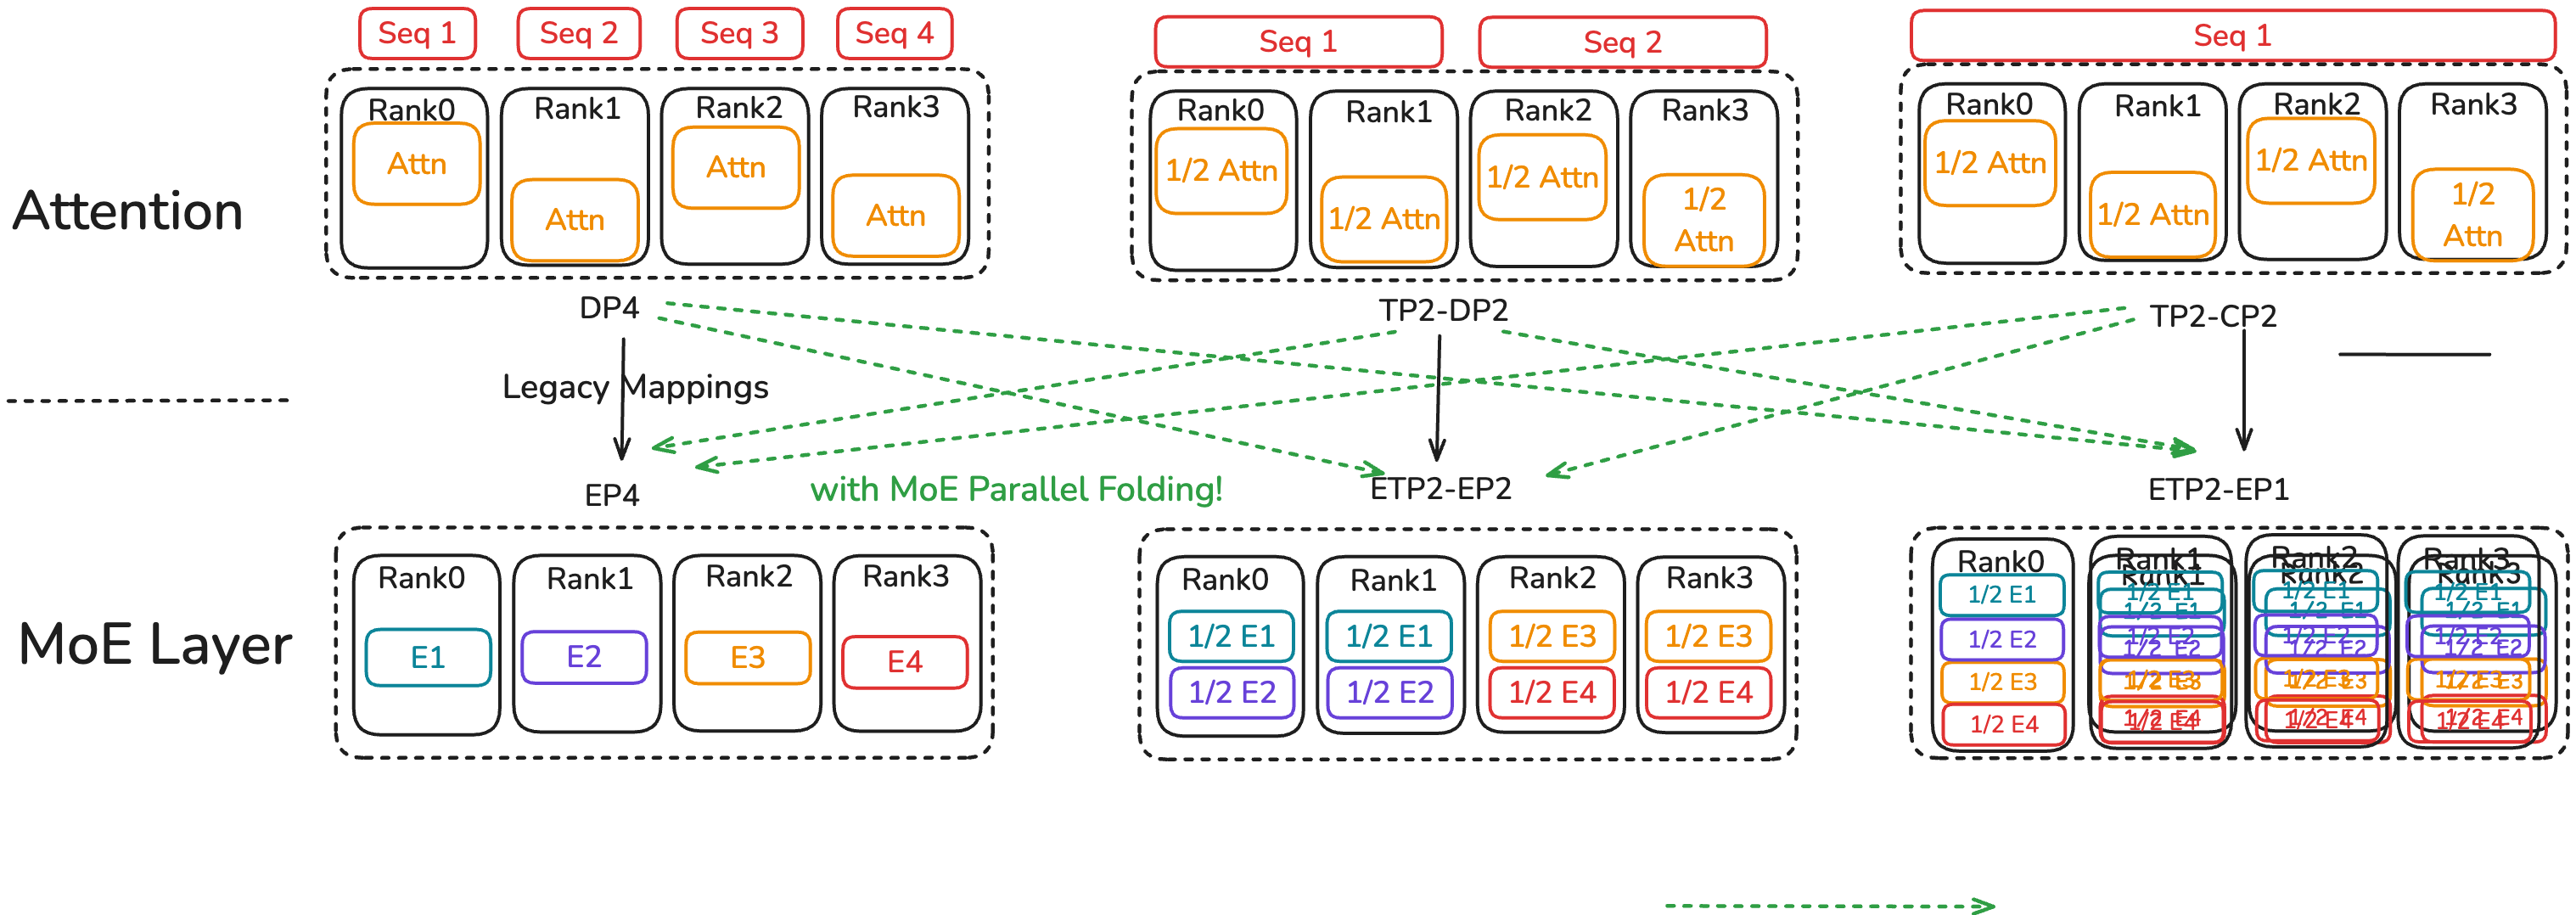
\includegraphics[width=0.9\textwidth]{moe-plots/Parallel-Folding-Paper/MoE_Parallel_Folding-mapping-switch.excalidraw.png}
    \caption{并行映射：传统约束与 MoE 并行折叠解耦。}
    \label{fig:moe-parallel-folding}
\end{figure}

并行折叠为注意力层和 MoE 层引入了单独的并行组：

\begin{itemize}
    \item \textbf{注意力层} 形成小组 $\text{TP} \times \text{CP} \times \text{DP} \times \text{PP}$，针对序列级密集计算进行了优化。
    \item \textbf{MoE 层} 形成小组 $\text{ETP} \times \text{EP} \times \text{EDP} \times \text{PP}$，其中 ETP（专家张量并行）和 EDP（专家数据并行）是 MoE 特定的维度。
\end{itemize}

唯一的约束： \textbf{管道并行度 (PP) 必须保持一致} 跨两种布局，以确保正确的梯度流通过模型。
\subsubsection{完整的多维并行堆栈}\label{sec:multi-dim-parallelism}

以并行折叠为基础，Megatron-Core 精心策划了五个并行维度：

\begin{center}
\begin{tabular}{lll}
\toprule
\textbf{方面} & \textbf{适用于} & \textbf{目的} \\
\midrule
TP（张量） & 注意力 & 分片大型 QKV/投影矩阵 \\
CP（上下文） & 注意力 & 分配长序列 \\
DP（数据） & 注意力 & 处理不同批次 \\
PP（管道） & 两个都 & 按层拆分模型（必须一致） \\
\midrule
EP（专家） & MoE & 跨 GPU 分配专家 \\
ETP（专家张量） & MoE & 专家内部分片（很少使用） \\
EDP​​（专家数据） & MoE & 复制专家的吞吐量 \\
\bottomrule
\end{tabular}
\end{center}

\textbf{关键配置原则}:
\begin{itemize}
    \item \textbf{注意力层}：针对大型矩阵（高 TP）和长序列（高 CP）进行优化。
    \item \textbf{MoE 层}：针对许多小专家进行优化（高EP，通常ETP=1）。
    \item \textbf{PP（管道并行）}：两者必须保持一致，以确保正确的数据流。
\end{itemize}

除了上述并行策略之外（\figref{fig:parallel-folding-detailed}），Megatron-Core 的并行折叠框架还集成了分布式优化器和具有 EP 支持的 FSDP，以进一步减少内存占用：

\textbf{分布式优化器+EP。} 每个等级中只有本地专家的权重和梯度；优化器状态在同一 Expert 的副本之间进行分片（通过 EDP）。这消除了非本地专家的冗余优化器内存，并将梯度同步限制在最小组内。

\textbf{FSDP + EP。} 为了实现更高的内存效率，Megatron-Core 的定制 FSDP (Megatron-FSDP) 通过双 DeviceMesh 架构跨数据/专家组完全分片参数、梯度和优化器状态，​​减少内存占用，同时将 AllGather 和 ReduceScatter 与计算重叠。它兼容 TP/EP/CP 和混合精度（BF16、FP8、FP4）。看 \secref{sec:fsdp-ref} 以获得完整的设计。

\subsubsection{并行折叠的好处}

如图所示 \figref{fig:moe-parallel-folding}，MoE 并行折叠消除了 $\text{EP} \leq \text{DP}$ 的限制，因为它允许 EP 在注意力并行配置的任意子组上“折叠”。这提供了四个关键优势：

\begin{enumerate}
    \item \textbf{打破EP $\leq$ DP约束}：EP 现在可以通过折叠 TP 来超过 DP$\times$CP组。考虑配置为 TP=4、CP=2、DP=8、PP=4（总共 256 个 GPU）的注意力：
    \begin{itemize}
        \item 繁体：EP $\leq$ DP = 8，因此最大 EP 为 8。
        \item 对于并行折叠：MoE 使用 ETP=1、EP=64、EDP=1（相同 PP=4）。 EP“折叠”穿过 TP$\times$CP$\times$DP 组，启用 8$\times$ 更高的专家并行性，同时注意力层保持最佳 TP=4、CP=2 配置。
    \end{itemize}
    
    \item \textbf{降低最低 GPU 要求}：CP=8、EP=8 的传统配置至少需要 64 个 GPU。通过 Folding，CP 和 EP 共享相同的 GPU 组，仅需要 8 个 GPU。
    
    \item \textbf{实现独立优化}：Attention 可以对大型矩阵使用高 TP，而 MoE 使用 ETP=1 以获得完整的专家宽度和更好的 GEMM 效率。
    
    \item \textbf{在 NVLink 域中保持高带宽通信}：CP（用于注意力）和 EP（用于 MoE）全对全通信都可以保留在 NVLink 连接的 GPU 组内，从而避免较慢的跨节点传输。
\end{enumerate}

% fix typo
\begin{figure}[ht]
    \centering
    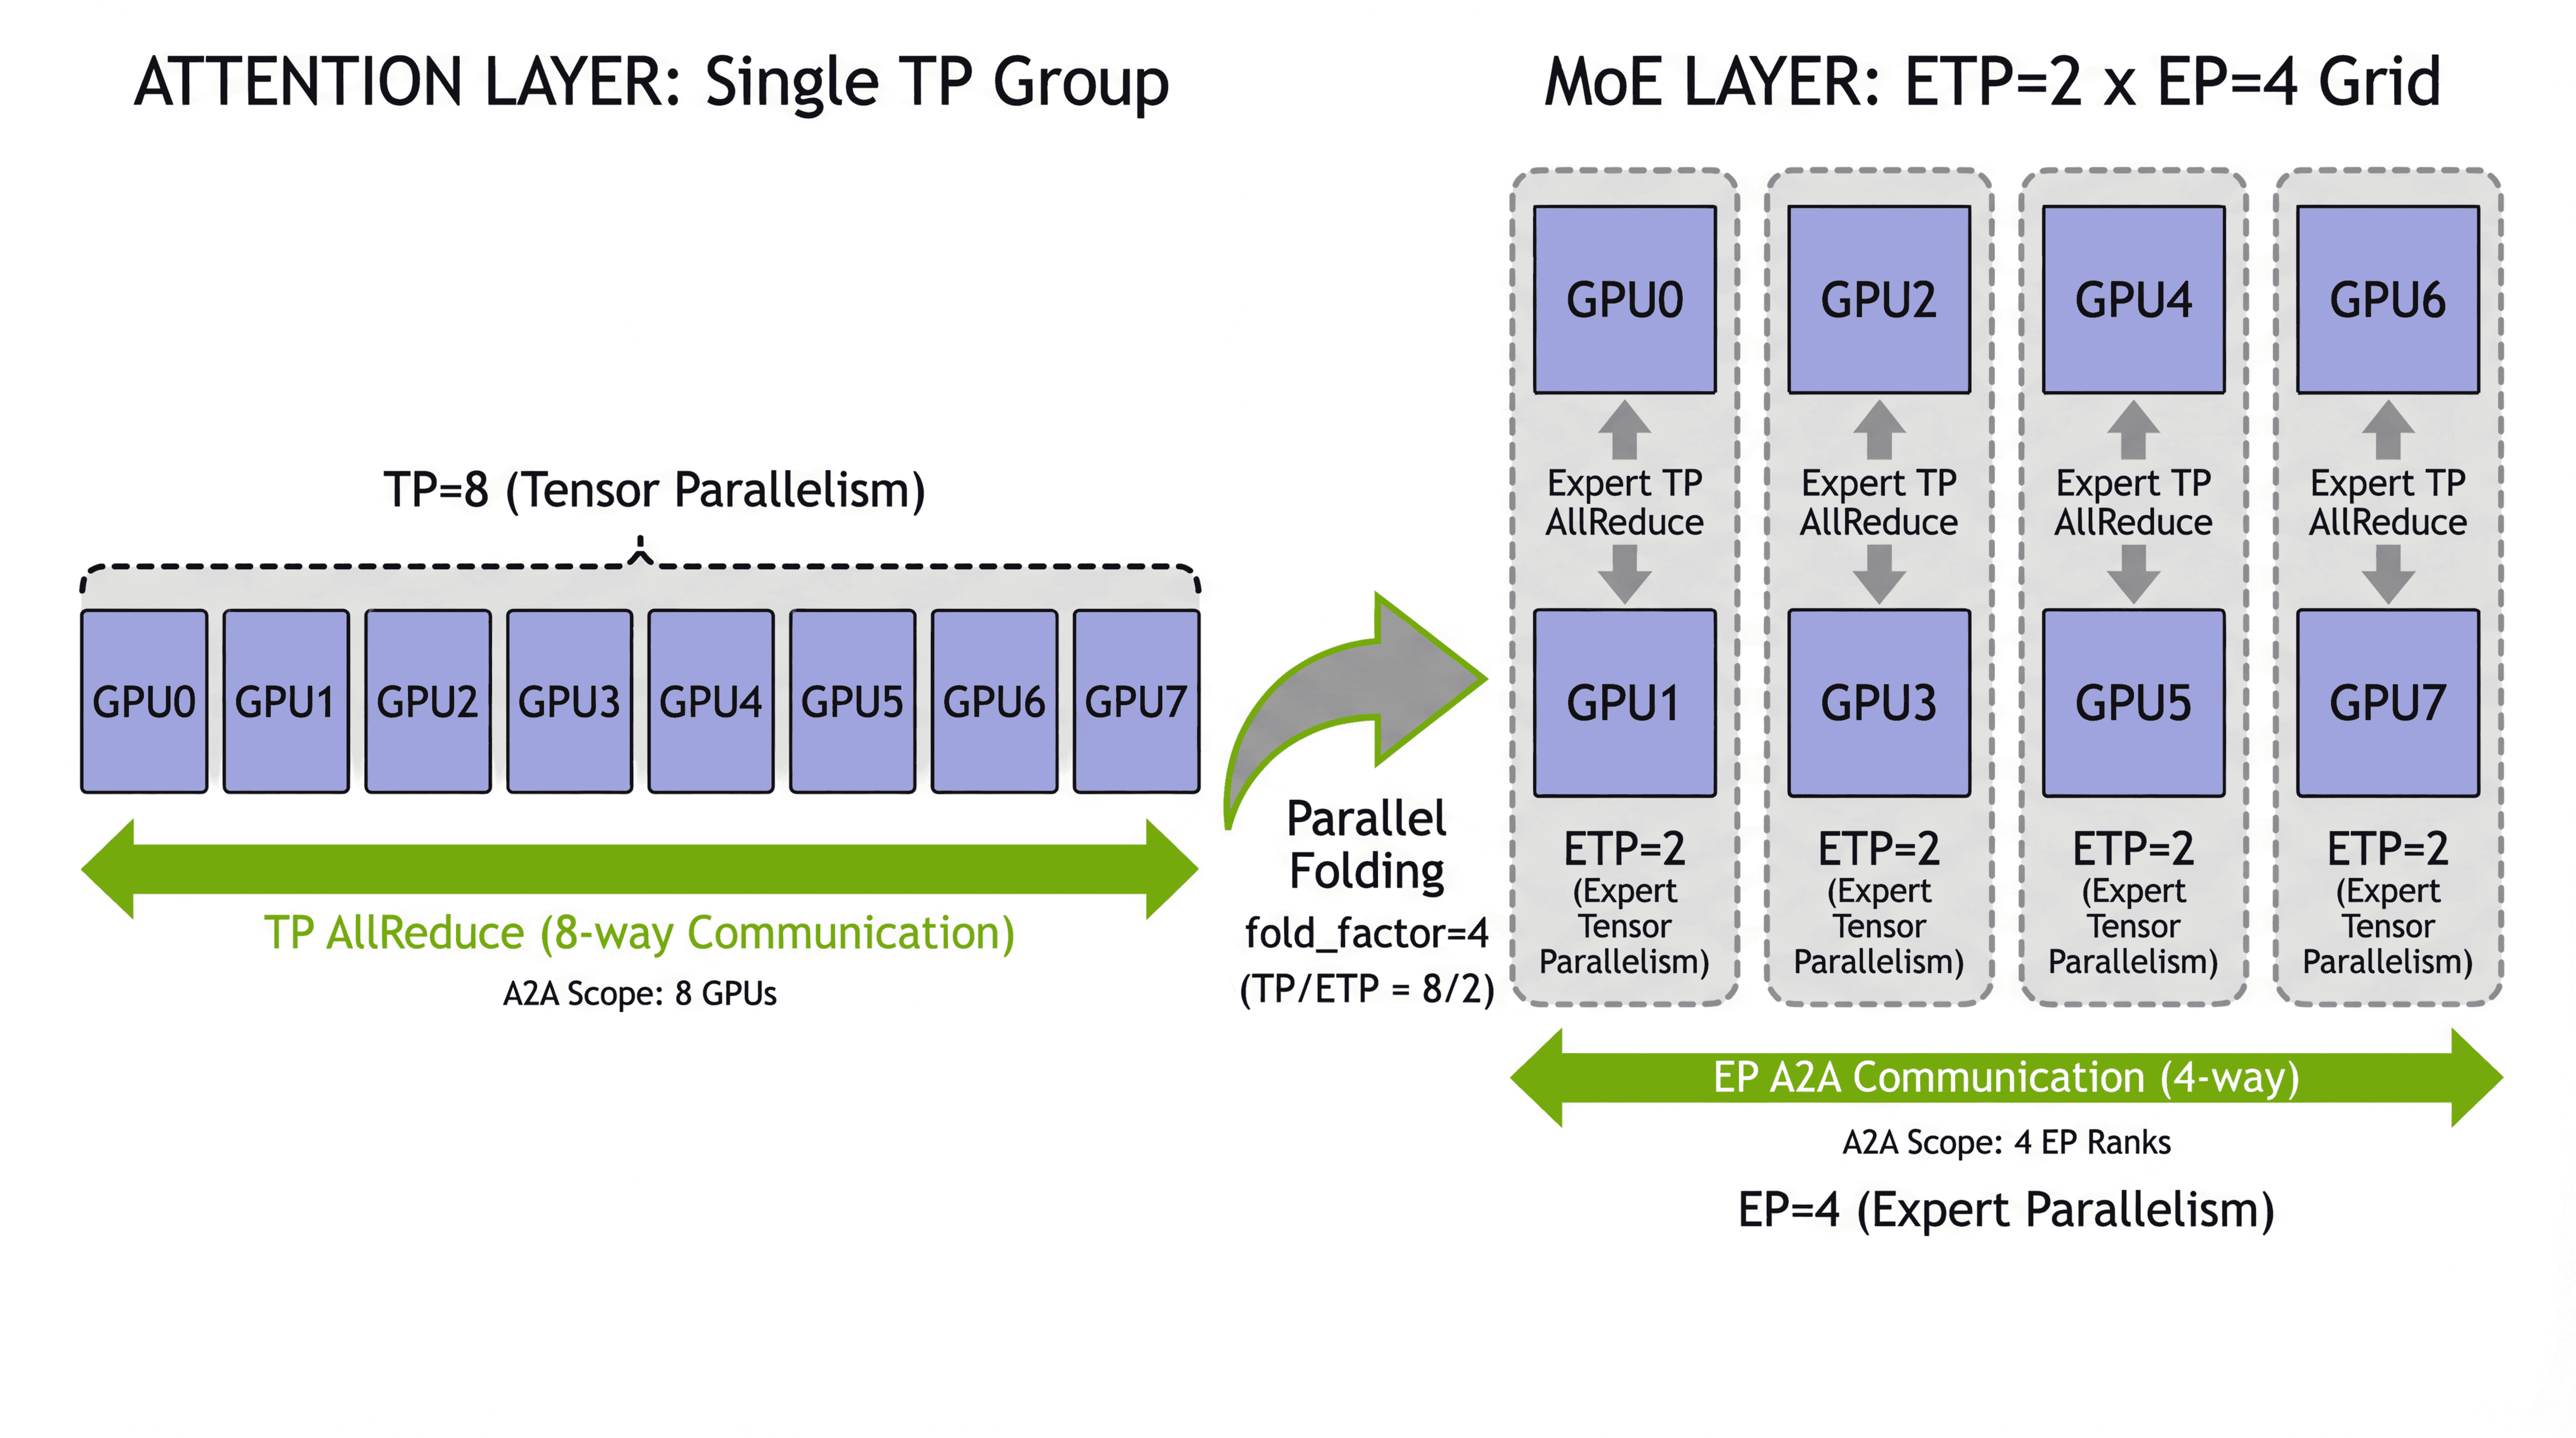
\includegraphics[width=0.9\textwidth]{figures/plots/parallel_folding_detailed_draft.png}
    \caption{并行折叠：解耦注意力和 MoE 并行映射。}
    \label{fig:parallel-folding-detailed}
\end{figure}

\subsubsection{概括}

本节讨论了 \emph{分销挑战} 用于MoE 训练。核心问题是 \emph{稠密-稀疏失配}，根源于 MoE 的稀疏性：注意力层和 MoE 层具有冲突的最佳并行配置，但先前的框架迫使它们共享一种配置。 \textbf{MoE 并行折叠} 通过解耦并行映射来解决这个问题，允许注意力使用高 TP/CP，而 MoE 独立使用高 EP。 Megatron-Core 与分布式优化器和 FSDP 一起将所有并行维度编排到一个统一框架中，将 MoE 训练扩展到数千个 GPU。

然而，仅可扩展的分布并不能保证训练效率。第~节中确定的三个基本障碍\ref{sec:challenges}内存、通信和计算效率墙仍然必须解决。以下部分介绍了Megatron Core突破这些墙壁的解决方案。

\section{扩展 MoE：打破内存、通信和计算效率壁垒}\label{key-features-optimizations}

部分~\ref{parallelism-strategies} 已确立的 \emph{如何} 在数千个 GPU 上分配 MoE 训练。本节地址 \emph{如何提高效率}。挑战是巨大的：节~\ref{sec:challenges} 确定了由 MoE 稀疏驱动的参数计算不匹配而出现的三个基本障碍（内存墙、通信墙和计算效率墙）。这些墙不仅带来不便，而且还带来了麻烦。如果不解决这些问题，训练大规模 MoE 模型要么不可行（内存），要么速度极慢（通信、计算）。

\textbf{为什么是这三堵墙？} 这些障碍来自 GPU 加速训练的基本资源：内存存储参数和激活、互连在设备之间传输数据以及计算单元执行操作。每个训练系统都必须获得足够的内存，将数据移动到需要的地方，并有效地执行计算。其他潜在的瓶颈，例如用于检查点或主机端数据加载的存储 I/O，也存在，但运行的时间尺度允许它们与训练迭代重叠。三堵墙代表了每次前后传递的严格限制。

\textbf{墙壁相互作用。} 这些挑战并不是独立的；它们形成了一个紧密耦合的系统，修复一堵墙可能会暴露或恶化另一堵墙。考虑一个具体的优化轨迹：训练 1000B MoE 模型的团队首先遇到内存墙：仅激活就超过了 GPU 容量。它们启用激活重新计算（第~\ref{sec:memory-wall}），通过在向后传递过程中重新生成激活来交换内存以进行计算。内存限制得到解决，分析显示现在全面通信占据主导地位；计算墙隐藏了通信墙。他们实现了通信-计算重叠（第~\ref{sec:comm-wall}），通过专家执行来管道化所有到所有的传输。但细粒度专家的完成速度比通信速度快，从而限制了重叠效率。它们可以实现降低精度的训练（第~\ref{sec:reduced-precision-training}）以减少内存占用，允许更大的批处理大小，从而提供更多的计算来隐藏通信。这是可行的，但引入了量化内核，它会分割执行流并增加内核启动开销。系统变为主机绑定：GPU 在内核启动之间空闲。他们部署 CUDA 图形（部分~\ref{sec:compute-wall}）以减少启动开销，但图需要静态张量形状，这与无丢包路由的动态专家分配相冲突。每个解决方案都会在系统中产生涟漪，要求同时了解所有三堵墙。孤立地解决墙壁问题会导致解决方案次优；有效的优化需要将内存、通信和计算视为一个统一的系统。

Megatron-Core 通过集成系统设计解决了这些挑战。本节的其余部分介绍了按其主要解决的墙组织的解决方案：
\begin{itemize}
    \item \textbf{部分~\ref{sec:memory-wall}：打破内存墙。} 我们如何在 GPU 内存限制内适应训练？本节涵盖激活管理、重新计算策略、卸载和分布式参数存储。
    \item \textbf{部分~\ref{sec:comm-wall}：打破通信壁垒。} 我们如何最大限度地减少设备间通信损失的时间？本节涵盖优化调度程序、通信计算重叠和管道集成。
    \item \textbf{部分~\ref{sec:compute-wall}：打破计算效率壁垒。} 我们如何保持 GPU 的工作饱和度？本节介绍内核融合、CUDA 图和无滴 MoE 的无同步执行。
\end{itemize}

FP8/FP4 中的降低精度训练可同时在所有三堵墙上提供优势，在第 1 节中单独介绍~\ref{sec:reduced-precision-training}。长上下文 MoE 训练会在注意力主导计算时改变优化平衡，在第 5 节中进行了讨论~\ref{sec:long-context-training}.

\subsection{打破内存墙}\label{sec:memory-wall}

内存是 MoE 训练中的第一个硬约束：如果参数、优化器状态和激活的组合占用空间超过 GPU 容量，则训练无法继续。随着模型和专家数量的增长，内存需求快速增长，这使得内存优化对于实际训练至关重要。理解 \emph{在哪里} 内存消耗对于有效的优化至关重要。

\subsubsection{内存剖析：内存消耗的来源}

由于几个不同的开销来源，MoE 模型通常比同等的密集模型消耗更多的内存。考虑使用 BF16 精度训练的 DeepSeek-V3 $\text{PP}4 \times \text{VPP}4 \times \text{EP}64$ 跨 256 个 GPU 的配置。表~\ref{tab:memory-breakdown} 显示了每个 GPU 内存细分，显示总需求为 199.5 GB，远远超出未经优化的 H100 GPU 的 80 GB 容量。

\begin{table}[ht]
\centering
\caption{使用 BF16 训练的 DeepSeek-V3 每个 GPU 的内存细分（$\text{PP}4 \times \text{VPP}4 \times \text{EP}64$，256 个 GPU）。}
\label{tab:memory-breakdown}
\begin{tabular}{lrl}
\toprule
\textbf{成分} & \textbf{每个 GPU 的内存} & \textbf{优化技术} \\
\midrule
重量 \& 渐变 & 36.4GB & PP、EP 或 TP 分片 \\
主要重量 \& 优化器状态 & 32.1GB & 分布式优化器，BF16矩 \\
激活 & 131.0GB & 低精度、重新计算、卸载 \\
\midrule
\textbf{全部的} & \textbf{199.5GB} & \\
\bottomrule
\end{tabular}
\end{table}

三个组成部分促成了这一足迹：

\textbf{权重和梯度 (36.4 GB)。} 全部 $E$ 专家参数必须保留在内存中，即使只有 $K$ 激活每个令牌。 DeepSeek-V3 具有 top-8 路由的 256 个专家说明了这一点：685B 个参数，但每个令牌仅激活 37B，即 18 个$\times$ 差距。

\textbf{优化器状态 (32.1 GB)。} Adam 存储每个参数的动量和方差，使 FP32 中的参数内存增加三倍。使用 BF16 矩的混合精度训练减少了这种开销，但并没有消除它。

\textbf{激活 (131.0 GB)。} 最大的内存消耗，超过了权重和优化器状态的总和。 MoE 激活随着层深度、隐藏维度和顶部而缩放$k$，以及批量大小和序列长度。这使得激活成为主要优化目标。

\begin{notebox}
在大规模 MoE 训练中，激活主导着内存消耗，通常超过权重、梯度和优化器状态的组合内存。这使得激活内存优化成为实现更大批量或更灵活并行配置的最高优先级。
\end{notebox}

其他 MoE 特定因素会增加内存压力：动态路由可能会造成负载不平衡，某些专家会暂时收到太多令牌，并且通常必须填充令牌以适应高效的计算内核，从而消耗超出实际数据的内存。这些是激活内存成本，可以通过下面讨论的重新计算技术来降低。 ECHO 进一步解决了负载不平衡问题（第~\ref{sec:echo}），动态克隆热门专家以平衡不同级别的令牌分配。

无法通过更改模型架构来减少内存，因此优化必须针对数据的存储和管理方式。四种互补策略可解决内存限制：

\begin{enumerate}
    \item \textbf{降低存储精度。} 较低精度的格式（FP8/FP4 而不是 BF16）可减少激活内存，同时对精度的影响最小。内存高效排列完全消除了冗余的中间张量。
    \item \textbf{用计算换取存储。} 激活重新计算 \cite{chen2016training,korthikanti2022reducingactivationrecomputationlarge,beaumont2021optimal} 在前向传递过程中丢弃中间结果，并在向后传递过程中重新生成它们，以计算周期换取内存容量。
    \item \textbf{卸载到主机内存。} 当 GPU 内存耗尽时，激活可以在前向传递期间传输到 CPU 内存，并在后向传递期间检索，用 PCIe 带宽换取 GPU 内存 \cite{ren2021zerooffload}.
    \item \textbf{跨设备分发。} 完全分片数据并行 (FSDP) \cite{zhao2023pytorchfsdp,rajbhandari2020zero,rajbhandari2021zeroinf,rajbhandari2023zeropp} 跨数据并行等级划分参数、梯度和优化器状态，​​从而能够训练超出单设备容量的模型。 
\end{enumerate}

以下小节将这些技术分为两组。首先，按开销排序的激活内存优化：零开销（内存高效排列）、精度权衡（FP8/FP4 与 BF16）、计算权衡（重新计算）和带宽权衡（卸载）。然后，针对权重和优化器状态的优化：精度感知优化器和分配策略（FSDP）。

\subsubsection{内存高效排列：零开销激活减少}\label{sec:mem-eff-permute}

最理想的内存优化是那些没有计算开销的优化。内存高效排列通过简单的代数重排消除冗余的中间张量来实现这一点。该技术是零开销的，因为它只是改变 \emph{什么时候} 应用路由器概率，而不是 \emph{无论} 它们被应用；在传统的实现方式中，向后传递所需的预激活缓冲区无论如何都会被存储。

正如章节中所描述的~\ref{sec:moe-layer-architecture}，路由器将每个令牌分配给其顶部$k$ 具有学习路由权重的专家，并且加权专家输出被组合以产生最终结果。

考虑一个令牌 $\mathbf{x}$ 路由到其top-$k$ 专家。让 $\mathcal{T}(\mathbf{x}) \subset \{1,\dots,E\}$ 用路由权重表示选定的专家集 $\{p_i\}_{i \in \mathcal{T}(\mathbf{x})}$。各位专家 $E_i$ 是一个带有权重矩阵的两层 MLP $\mathbf{W}_1^{(i)}, \mathbf{W}_2^{(i)}$ 和非线性激活 $\phi$ （例如，SwiGLU）：
\[
E_i(\mathbf{x}) = \mathbf{W}_2^{(i)}\,\phi\!\bigl(\mathbf{W}_1^{(i)}\mathbf{x}\bigr).
\]
在 \textbf{标准制定}，应用路由权重 \emph{后} 专家计算：
\begin{equation}\label{eq:moe-standard-combine}
\mathbf{y} = \sum_{i \in \mathcal{T}(\mathbf{x})} p_i \cdot \mathbf{W}_2^{(i)}\,\phi\!\bigl(\mathbf{W}_1^{(i)}\mathbf{x}\bigr).
\end{equation}
\textbf{内存高效排列} 吸收 $p_i$ 进入激活状态，应用它 \emph{前} 第二个线性层：
\begin{equation}\label{eq:moe-mem-eff-combine}
\mathbf{y} = \sum_{i \in \mathcal{T}(\mathbf{x})} \mathbf{W}_2^{(i)}\,\bigl(p_i \cdot \phi\!\bigl(\mathbf{W}_1^{(i)}\mathbf{x}\bigr)\bigr).
\end{equation}
当专家没有偏见条件时， $\mathbf{W}_2^{(i)}$ 是纯线性映射和标量乘法交换： $p_i \cdot \mathbf{W}_2^{(i)}\mathbf{h} = \mathbf{W}_2^{(i)}(p_i \cdot \mathbf{h})$ 对于任意向量 $\mathbf{h}$， 所以 \eqref{eq:moe-standard-combine} 和 \eqref{eq:moe-mem-eff-combine} 在数学上是等价的。


\begin{figure}[ht]
    \centering
    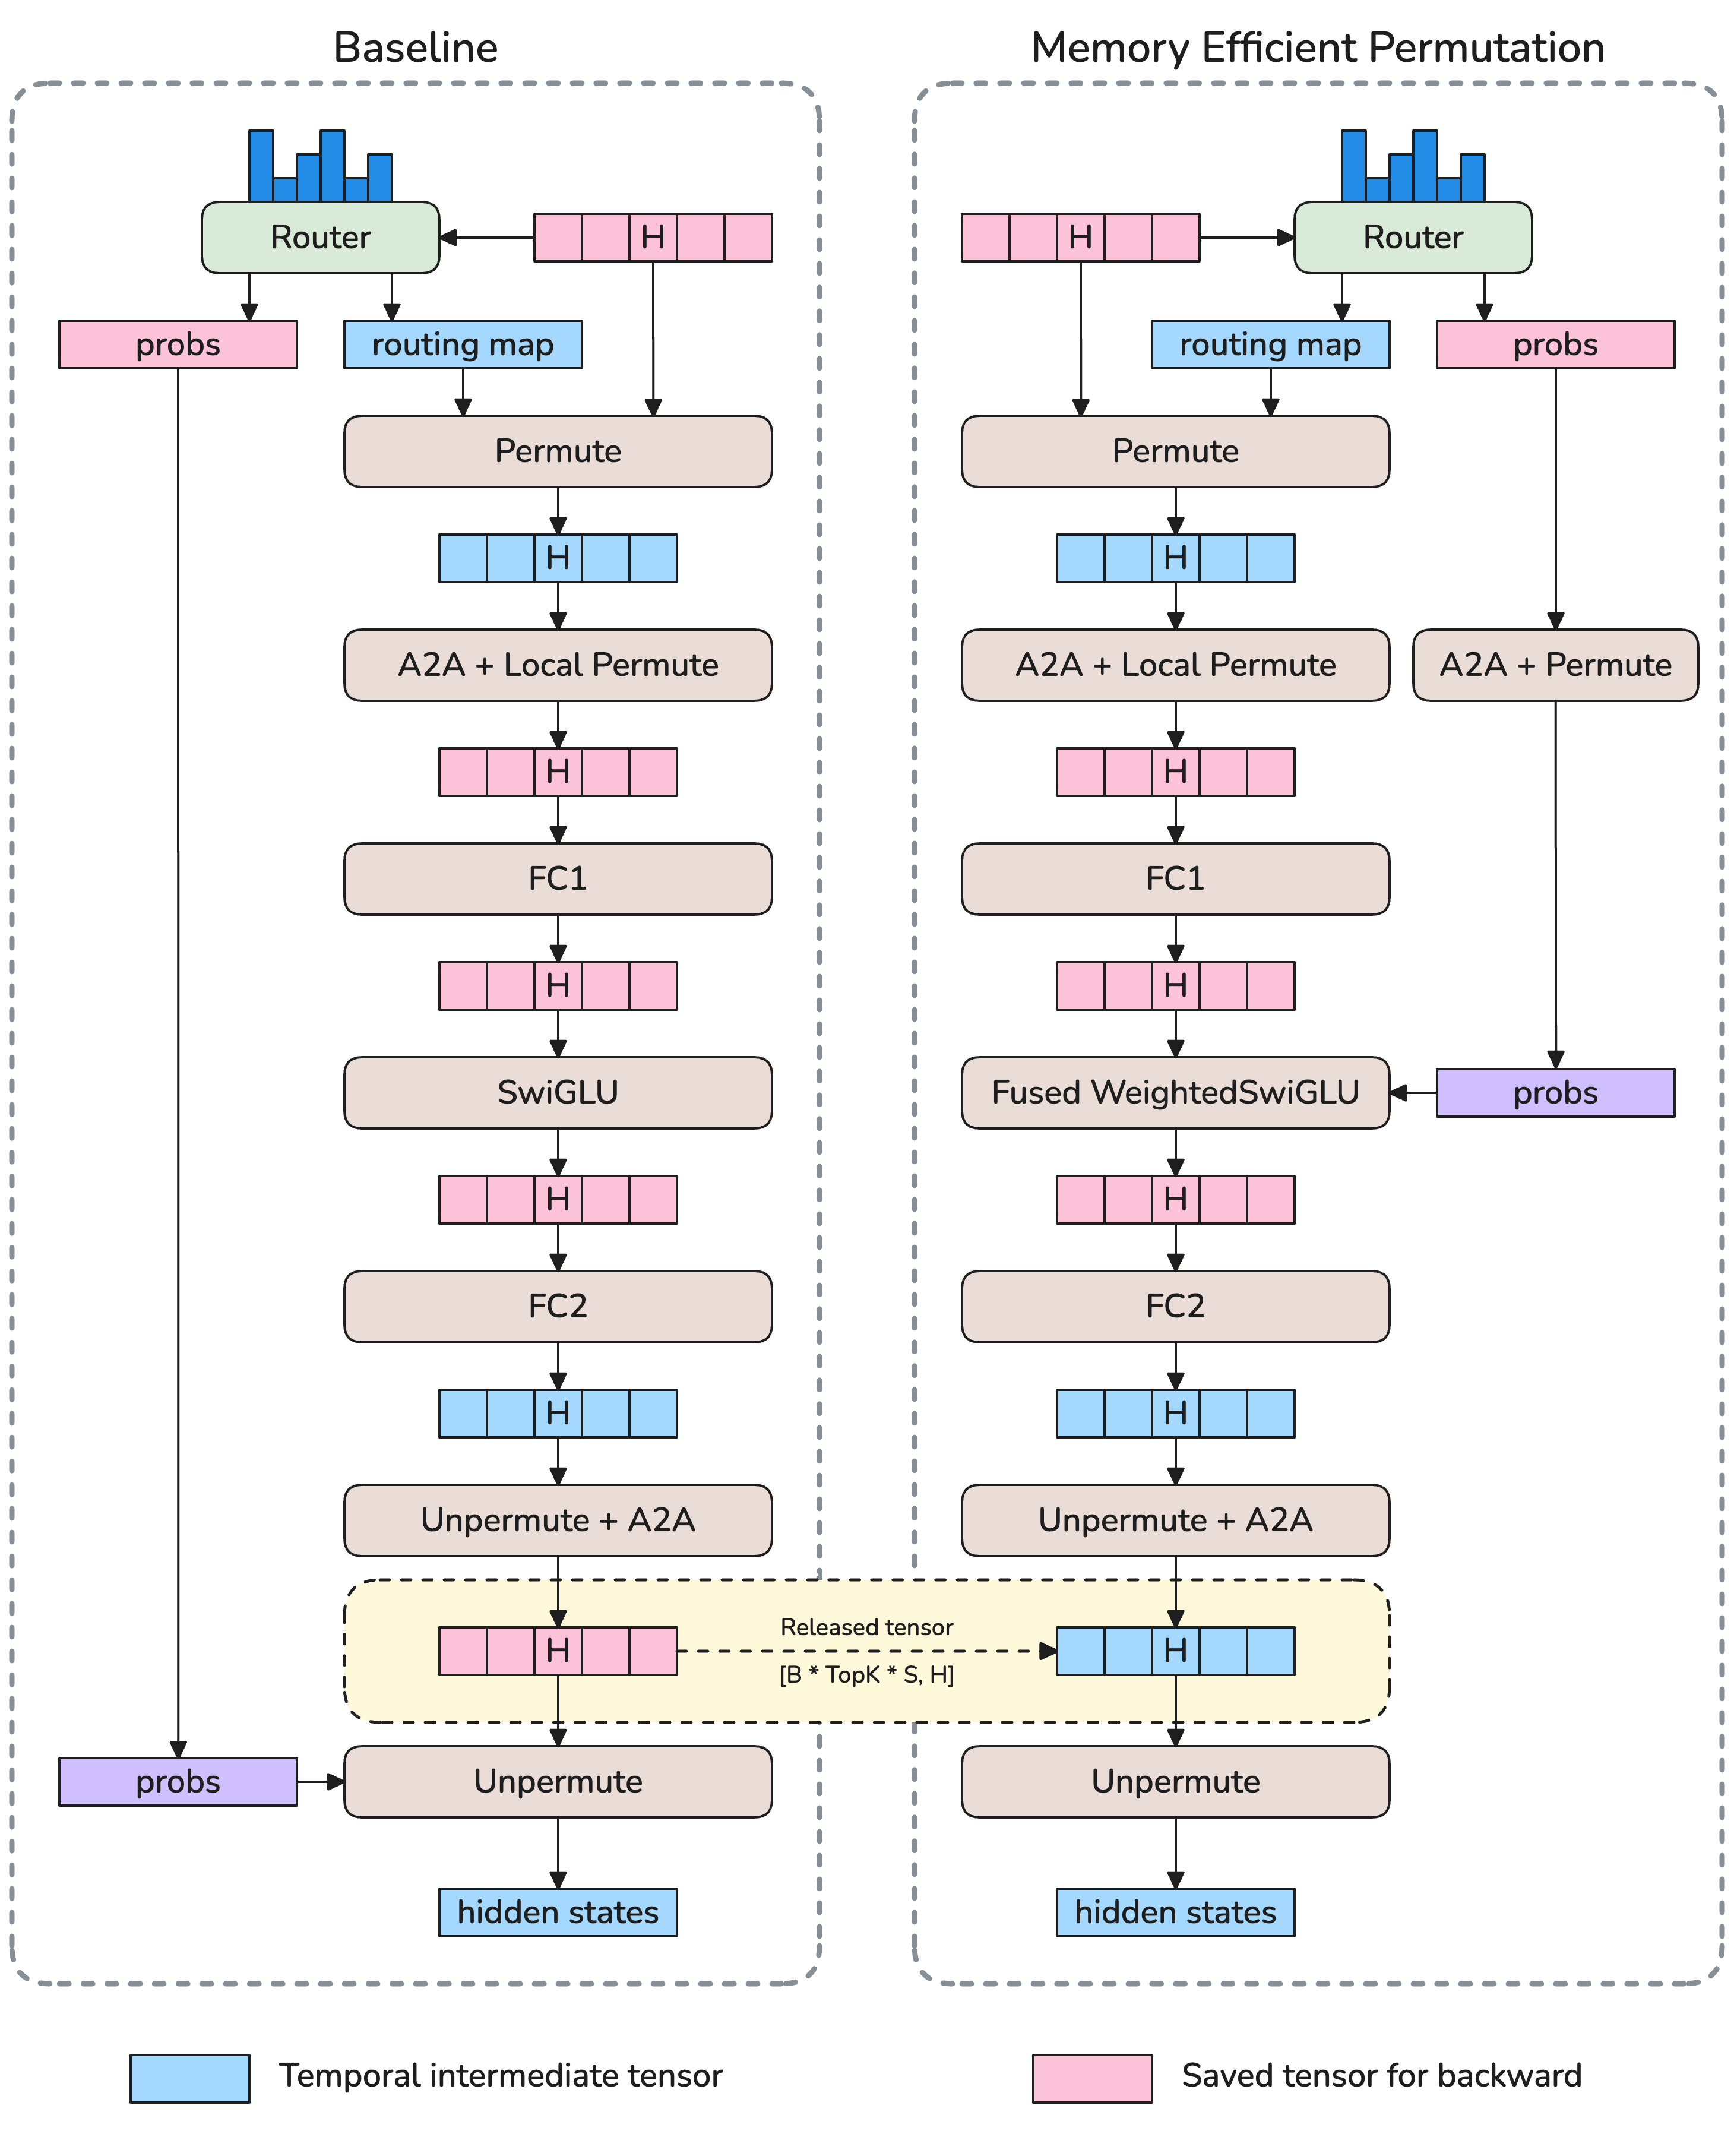
\includegraphics[width=0.6\linewidth]{figures/memory_efficient_permutation.png}
        \caption{内存高效排列。}
    \label{fig:mem-eff-permute}
\end{figure}

这种重新排列通过消除路由器向后传递所需的已保存张量来减少峰值内存。让 $\mathbf{z}_i = \mathbf{W}_1^{(i)}\mathbf{x}$ 表示预激活输入。在标准制定中，计算 $\partial \mathcal{L}/\partial p_i$ 需要保留每个专家的输出 $E_i(\mathbf{x})$ 整个向后传球。在内存效率公式中， $p_i$ 乘以 $\phi(\mathbf{z}_i)$ 直接，所以 $\partial \mathcal{L}/\partial p_i$ 仅取决于 $\phi(\mathbf{z}_i)$，融合后向内核重新计算 $\mathbf{z}_i$ 在飞行中。自从 $\mathbf{z}_i$ 无论是否使用内存高效排列，都必须已保存用于 SwiGLU 激活自身的后向传递，不会引入额外的缓冲区，从而在零计算开销的情况下产生峰值内存的净减少。 \Figref{fig:mem-eff-permute} 说明了这种转变。

对于 DeepSeek-V3（表~\ref{tab:memory-breakdown}），内存高效排列为每个 GPU 节省了大约 26.3 GB 的激活内存，显着减少且计算成本为零。

\subsubsection{降低精度训练：用于减少激活内存的 FP8/FP4}\label{sec:fp8-activation}

将激活存储在 FP8/FP4 而不是 BF16 中可以减少内存占用，同时对模型质量的影响最小。

在前向传递过程中，必须保留每个线性层的输入，以计算后向传递中的权重梯度。在 Transformer 模型中，这些线性层输入构成了大部分激活记忆：注意力投影（Q、K、V、输出）和 MLP 层（包括 MoE 中的专家 MLP）各自保存其输入以进行梯度计算。通过将这些输入张量存储在 FP8/FP4 而不是 BF16 中，每个张量的内存占用量减少了 50\%/75\%。

表中为DeepSeek-V3配置~\ref{tab:memory-breakdown}，启用 FP8 训练可减少大约 16 GB 的激活内存，相当于大约 12\% 131 GB 激活预算。这相当于将适合 FP8 存储的约 32 GB 线性层输入减半。其余的激活（注意力分数、标准化中间值、路由张量）要么需要更高的精度以实现数值稳定性，要么不跨前向-后向边界存储。这种减少与其他激活优化（例如重新计算和卸载）正交，允许将它们组合起来以实现累积节省。

\textit{有关降低精度训练机制的详细信息，包括配方、量化策略和 MoE 特定的优化，请参阅第~\ref{sec:reduced-precision-training}.}

\subsubsection{重新计算：用计算换取内存}\label{sec:recomputation}

激活重新计算（或激活检查点）是一种成熟的技术，它在前向传递期间丢弃中间激活并在向后传递期间重新计算它们 \cite{chen2016training}。然而，简单的全层重新计算可以添加 $\sim$33\% 计算开销，对于 MoE 层来说成本更高，因为重新计算专家计算也会重新触发 EP 的全对全通信。Megatron Core介绍 \textit{细粒度的} 仅针对内存最密集但计算成本最低的操作进行重新计算，以最小的开销实现显着的内存节省 \cite{korthikanti2022reducingactivationrecomputationlarge}。

两种技术组成了该策略（\figref{fig:selective-recomputation}):

\begin{figure}[ht]
    \centering
    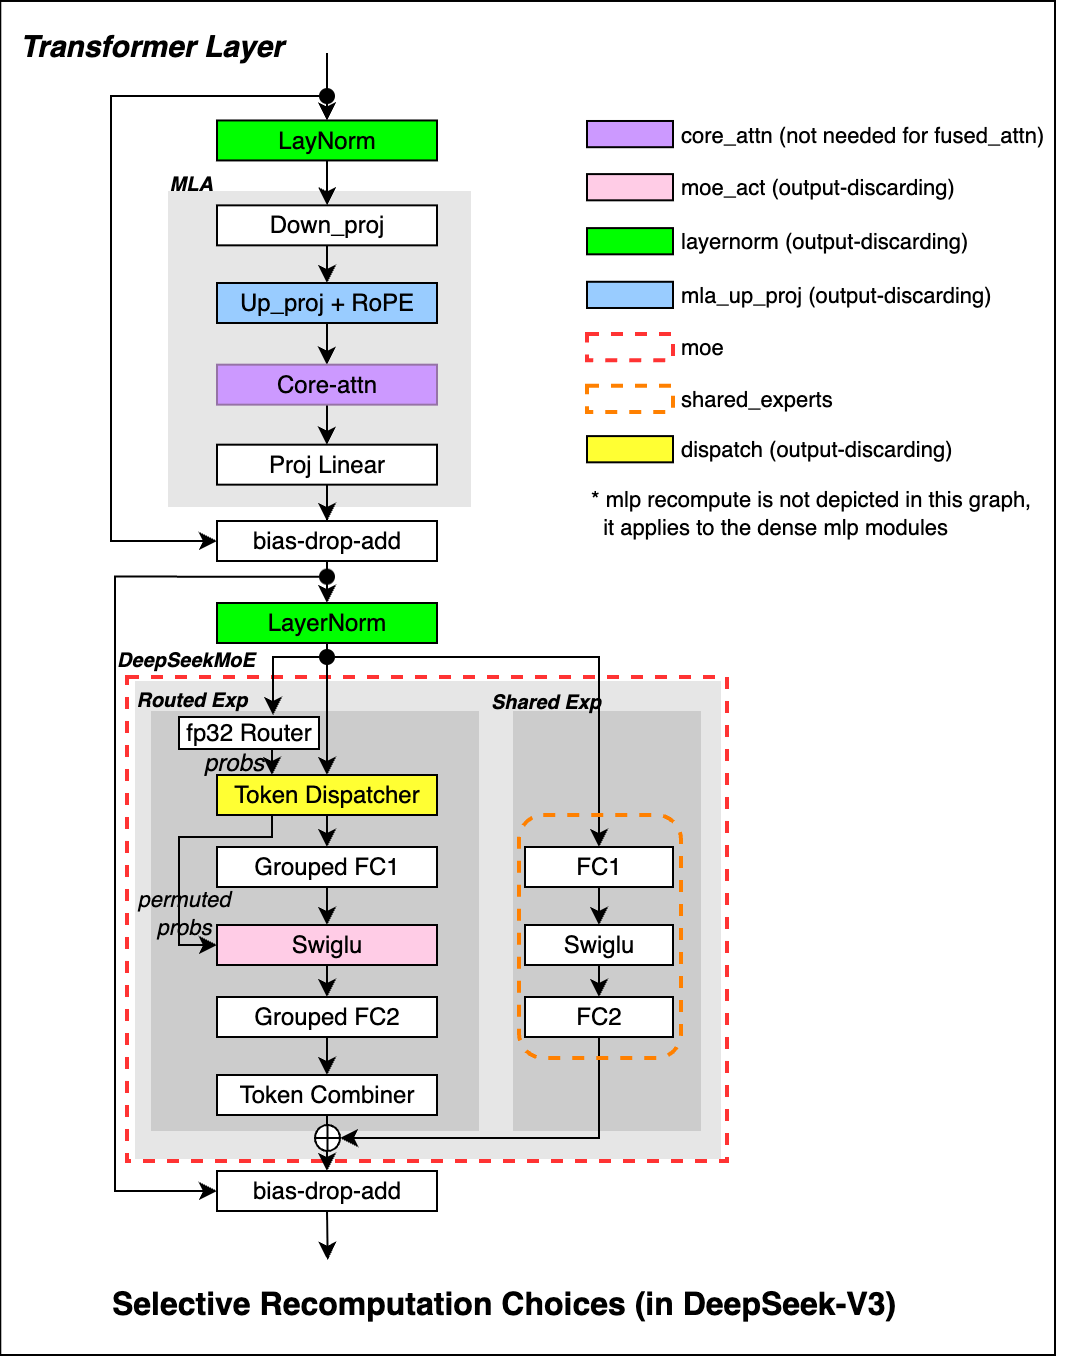
\includegraphics[width=0.5\linewidth]{figures/selective-recomputation.png}
        \caption{选择性重新计算。}
    \label{fig:selective-recomputation}
\end{figure}

\textbf{粒度重新计算。} 用户不是将激活检查点应用于大型整体部分，而是准确指定在向后传递中重新计算哪些计算。例如，可以仅重新计算专家 MLP 中的激活函数、LayerNorm 模块或多重潜在注意力 (MLA) 中的上投影。通过重新计算单个操作或子模块，只需适度增加计算工作量即可实现显着的内存节省，因为只有选定的部分需要重新计算（少于 5\% 额外的计算开销）。

\textbf{输出丢弃重新计算。} 传统的激活检查点工作流程将检查点模块的输出传递到下游层，存储这些输出以供反向传播使用。然而，由于这些输出将在向后传递期间重新计算，因此该存储是多余的。为了避免这种情况，Megatron-Core MoE 在被后续层消耗后立即释放检查点模块的输出。在向后传递期间，从重新计算的结果恢复输出。该策略确保不会为可以廉价恢复的激活保留不必要的内存，从而在不影响梯度正确性或训练动态的情况下减少内存占用。

表~\ref{tab:recomputation-savings} 表中总结了 DeepSeek-V3 配置的不同重新计算目标所实现的内存减少~\ref{tab:memory-breakdown}.

\begin{table}[ht]
\centering
\caption{通过 DeepSeek-V3 的细粒度重新计算减少每个 GPU 的内存（$\text{PP}4 \times \text{VPP}4 \times \text{EP}64$，256 个 GPU）。}
\label{tab:recomputation-savings}
\begin{tabular}{lr}
\toprule
\textbf{重新计算目标} & \textbf{每个 GPU 节省的内存} \\
\midrule
MLA 上投影 & 30.4GB \\
激活函数 (SwiGLU) & 3.8GB \\
层规范 & 8.2GB \\
\midrule
\textbf{全部的} & \textbf{42.4GB} \\
\bottomrule
\end{tabular}
\end{table}

\subsubsection{细粒度激活卸载}\label{sec:offloading}

% \footnote{This is collaborative work between NVIDIA and Rednote.} the footnote has been removed
当精度和重新计算优化后 GPU 内存仍然不足时， \textit{卸载} 激活 CPU 内存可提供额外的容量。与以计算周期换取内存的重新计算不同，卸载以 PCIe 带宽为代价。挑战在于隐藏计算背后的传输延迟，以便卸载看起来“免费”。

\paragraph{动机}
细粒度的 MoE 模型具有极端的参数膨胀：DeepSeek-V3 每个令牌仅激活 37B（18$\times$ 比例，表~\ref{tab:memory-breakdown}）； Kimi-K2 总计达到 1T，其中 32B 处于活动状态（31$\times$）。这个参数计算不匹配（小节~\ref{sec:challenges}) 对于卸载尤其严重，因为激活内存不会随着专家并行 (EP) 或管道并行 (PP) 的增加而减少；这些策略减少了参数记忆，而不是激活记忆。

Transformer Engine 提供层级卸载，但这种粗粒度限制了有效性。层内的不同模块具有显着不同的内存与计算比率：LayerNorm 激活很小且重新计算成本低廉，而 \texttt{expert\_fc1} 输入很大但计算成本很高。层级卸载无法区分这些情况。它要么卸载所有内容（浪费带宽），要么什么也不卸载（浪费内存）。

\paragraph{高级思想：重叠和预取。}
GPU 的复制引擎和计算引擎独立运行。当模块的计算时间超过其激活传输时间时，D2H副本可以零成本与后续计算同时运行。 \Figref{fig:activation-offloading-timeline} 说明了前向和后向传递的流重叠机制。

\begin{figure}[ht]
    \centering
    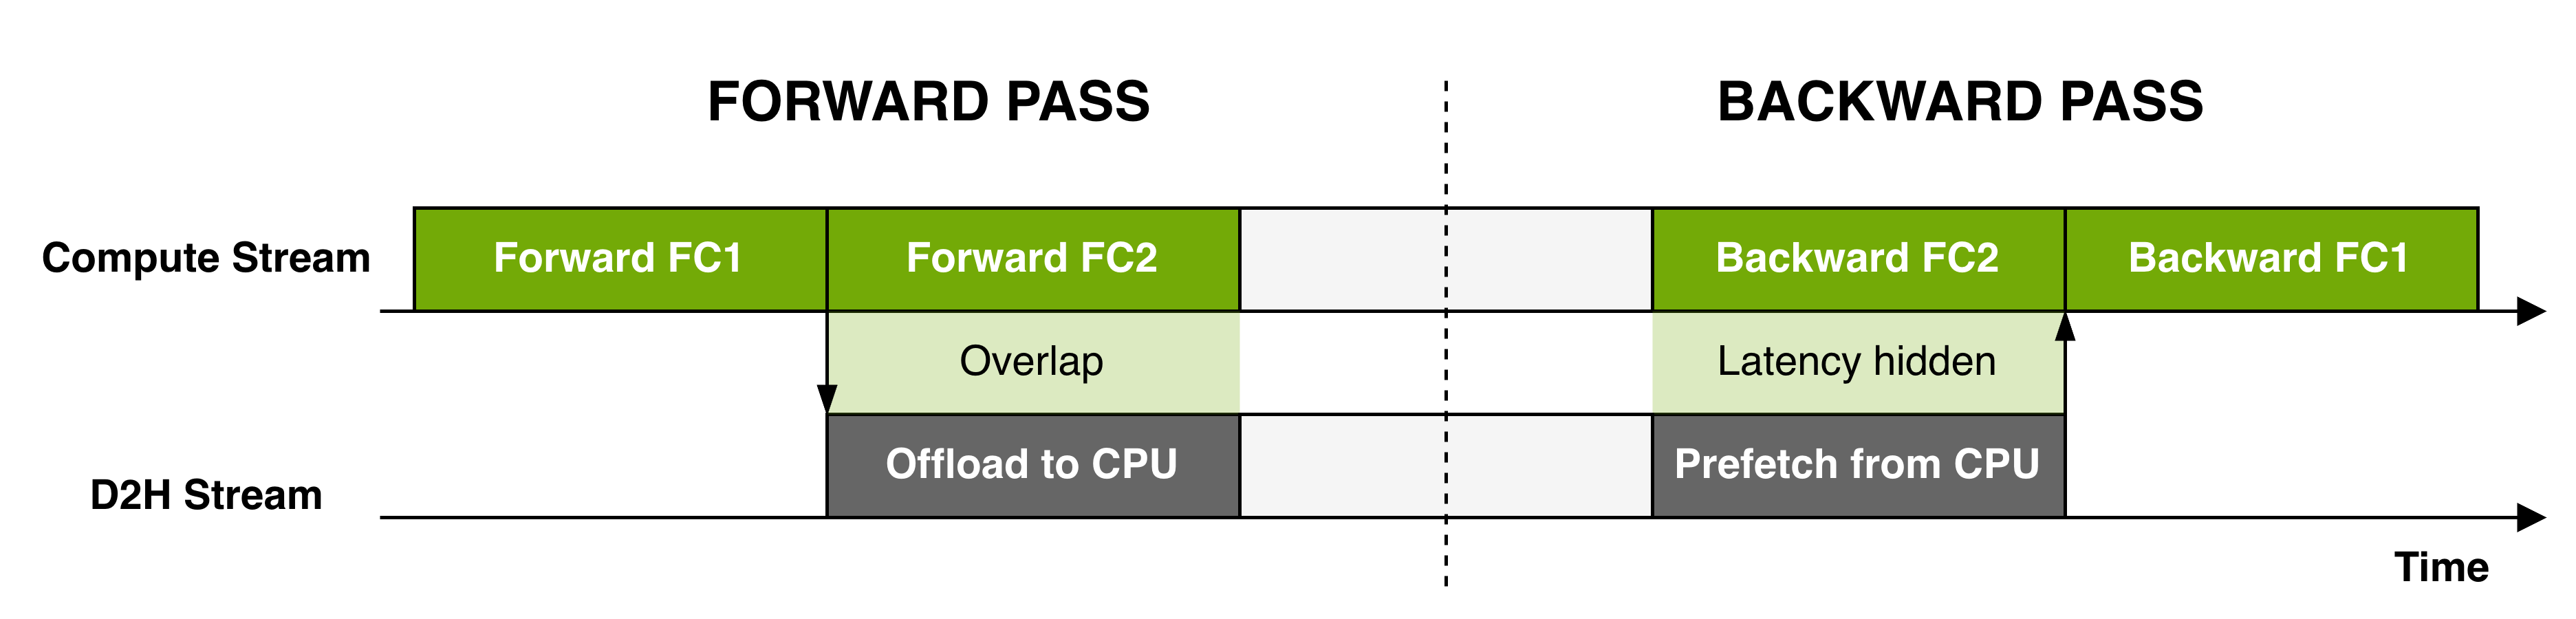
\includegraphics[width=0.9\textwidth]{figures/activation_offloading_timeline.drawio.png}
    \caption{细粒度激活卸载：前向和后向传递的流重叠。}
    \label{fig:activation-offloading-timeline}
\end{figure}

\paragraph{向前传球。}
在前向传播期间，输入激活在模块计算后立即卸载到 CPU，通过专用 D2H 流与下一个模块的计算并行运行。一个例外：最后一层的激活不会被卸载，因为在后向过程中立即需要它们，因此没有计算可用于隐藏传输延迟。

\paragraph{向后传球。}
在反向传播期间，激活重新加载遵循 \textit{层交错重载} 模式：系统重新加载同一模块的激活（例如， \texttt{expert\_fc1}）从 \textit{下一个} 层，同时计算当前层的梯度。发生重新加载 \textit{后} 每个模块都向后完成，因此每个模块类型在任何时候只有一个激活驻留在 GPU 内存中，从而避免了双倍激活存储的需要。当单个模块具有非常大的激活（其中 2$\times$ 内存占用会导致意外的内存峰值。

\paragraph{PP 和 VPP 处理。}
对于PP/VPP场景， \texttt{Chunk\-Offload\-Handler} 管理每个（微批次、VPP 阶段）组合的卸载/重新加载逻辑，与 PP=1 情况相同。主要挑战是管理虚拟管道块之间的数据依赖性和执行顺序。处理程序按倒序 (FILO) 排列到双端队列中，并按正序 (FIFO) 排列微批次。在向后过程中，弹出的处理程序会自动匹配 VPP 块执行顺序，从而将卸载的激活与其相应的向后传递正确配对。

\paragraph{主要技术特点。}
\begin{itemize}[itemsep=2pt,topsep=4pt]
    \item \textbf{模块级粒度：} 用户指定通过哪些模块卸载 \verb|--offload-modules|，启用混合策略。轻量级模块（LayerNorm、激活）使用重新计算，而昂贵的模块（注意、专家）则使用卸载。
    \item \textbf{异步传输：} 专用 D2H/H2D CUDA 流与计算并行运行传输； CUDA 事件仅在必要时协调同步。
    \item \textbf{重新计算积分：} 与细粒度重新计算相结合（\secref{sec:recomputation}）。为了 \texttt{moe\_act}，两种策略都适用：重新计算激活，同时卸载其输入，释放整个 \texttt{fc1}$\rightarrow$\texttt{act} 链。
    \item \textbf{CUDA 图形兼容性：} 使用外部事件而不是流同步，允许通过 CUDA 图形外部的计算隐藏卸载模块。
    \item \textbf{全场景兼容：} 支持PP=1/PP$>$1/VPP$>$1、所有精度（BF16/FP8/MXFP8/NVFP4）、具有全对全重叠的 1F1B 和 MoE/MLA 架构。
\end{itemize}

\paragraph{相对于完全重新计算的峰值内存优势。}
完整的重新计算存储每一层的 \textit{输入} 在 GPU 上，同时释放中间激活；向后根据这些存储的输入重新计算中间值。对于一个 $L$-层模型，GPU峰值显存为 $L \times \text{layer\_input} + 1 \times \text{layer\_intermediate}$。相反，卸载将层输入移至 CPU；在后退期间，每个输入在使用前重新加载并在使用后立即释放。这可将 GPU 峰值内存减少至 $1 \times \text{layer\_input} + 1 \times \text{layer\_intermediate}$，与模型深度无关。对于深度模型（例如 60 多个层），这代表了完全重新计算无法实现的基本内存优势。

\paragraph{表现。}
细粒度卸载和重新计算作为互补策略一起工作（\figref{fig:offloading-recomputation}）：像 LayerNorm 这样的轻量级操作使用重新计算，而像注意力和专家这样昂贵的模块则使用卸载。异步传输与计算重叠以隐藏 PCIe 延迟。表~\ref{tab:offloading-results} 显示多种配置的结果。细粒度卸载减少内存10--18\% 仅1.6--2\% 吞吐量开销。在训练Qwen3-235B的情况下，卸载可以降低张量并行度，这 \textit{改善} 吞吐量提高 15.0\% 具有几乎相同的内存成本。

\begin{table}[ht]
\centering
\caption{细粒度激活卸载对内存和吞吐量的影响。}
\label{tab:offloading-results}
\begin{tabular}{lccccc}
\toprule
\textbf{模型 \& 配置} & \textbf{基线} & \textbf{+卸载} & \textbf{内存 $\Delta$} & \textbf{吞吐量 $\Delta$} \\
\midrule
DeepSeek-V3完整版 & 169GB & 151GB & $-$10.7\% & $-$1.6\% \\
{\small TP1PP8EP32VPP4、MXFP8} & 945TF/秒 & 930TF/秒 & & \\
\midrule
Qwen3-235B  & 172GB & 175GB & $+$1.7\% & $+$15.0\% \\
{\small TP2$\rightarrow$TP1+EP16$\rightarrow$EP64} & 800 TF/秒 & 920TF/秒 & & \\
\bottomrule
\end{tabular}
\end{table}

\begin{figure}[ht]
    \centering
    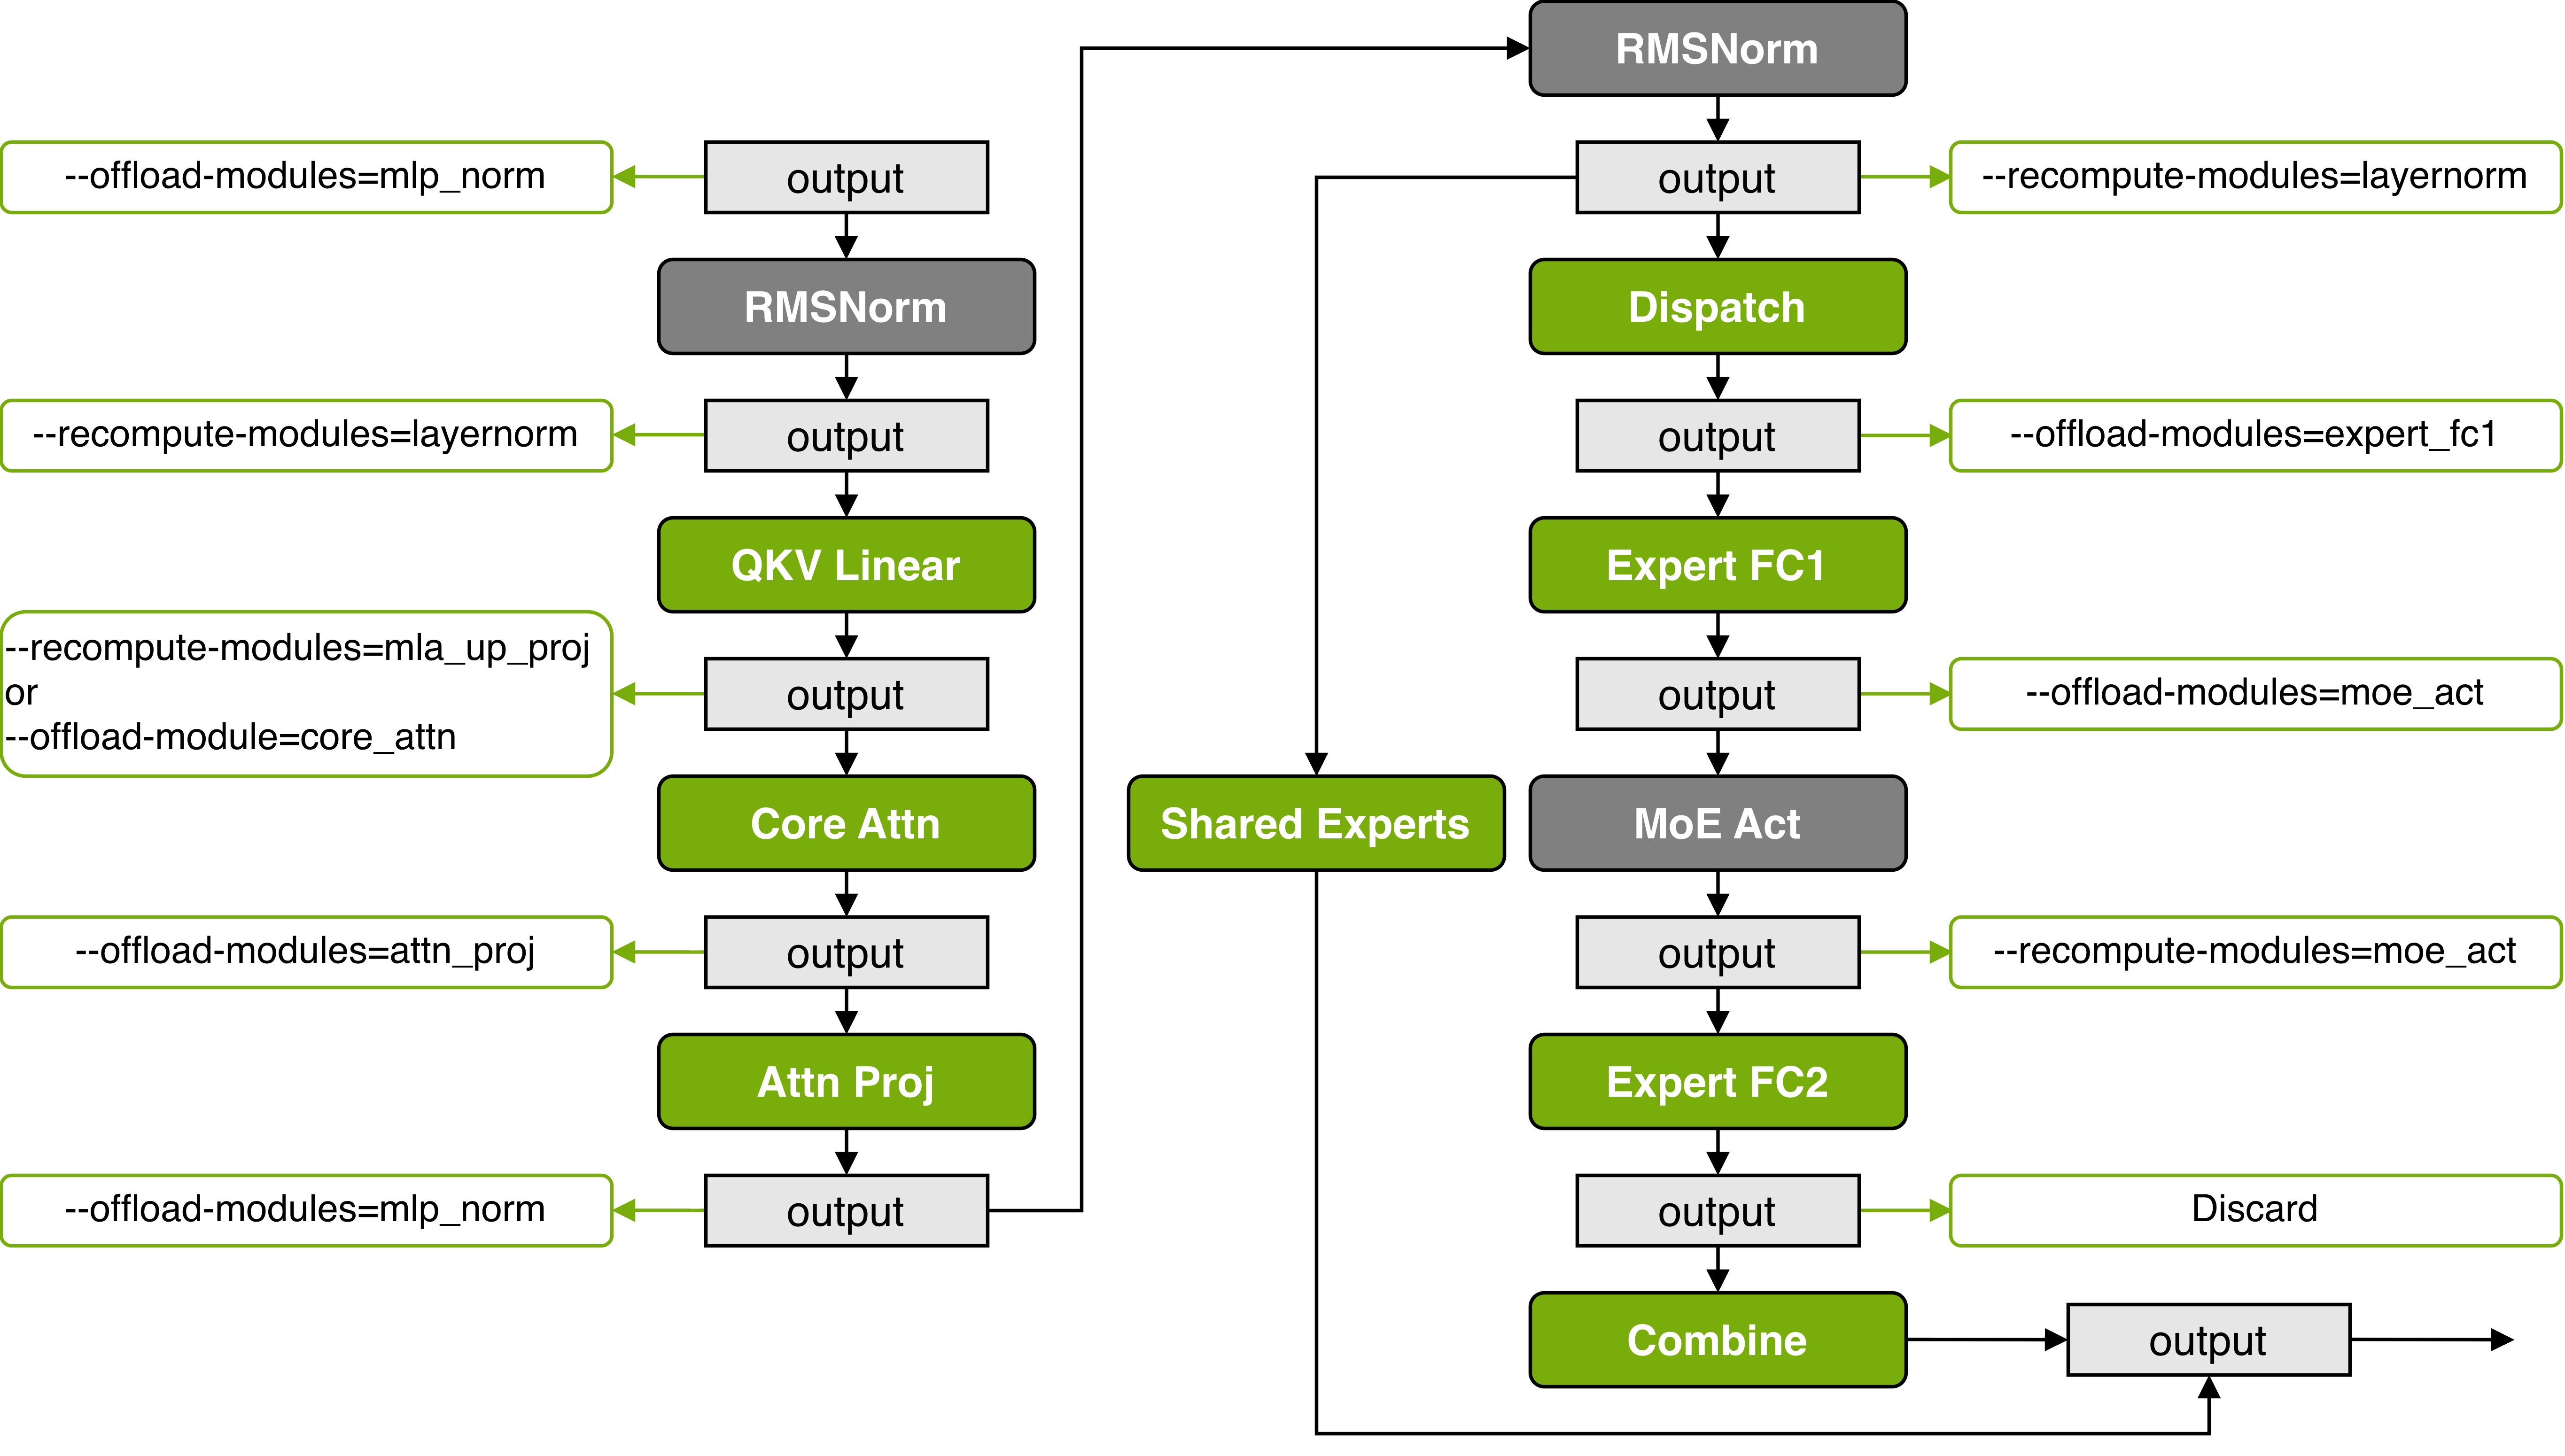
\includegraphics[width=0.8\linewidth]{figures/offloading_recomputation.png}
    \caption{细粒度卸载和重新计算：互补的内存优化策略。}
    \label{fig:offloading-recomputation}
\end{figure}

\subsubsection{权重和优化器优化：低精度存储和卸载}\label{sec:precision-opt}

前面的优化针对的是激活内存，它在内存崩溃中占主导地位。不过表~\ref{tab:memory-breakdown} 显示主要权重和优化器状态每个 GPU 消耗 32.1 GB，相当于 16\% 总内存占用量。对于具有数千亿参数的模型，该组件成为重要的优化目标。 Megatron-Core 提供两种技术：降低存储需求的精确感知优化，以及将非活动状态移出 GPU 的 CPU 卸载。

\paragraph{精度感知优化器。}
Adam 优化器 \cite{kingma2014adam} 每个参数维护两个状态张量：一阶矩 (\texttt{exp\_avg}) 和二阶矩 (\texttt{exp\_avg\_sq}）。传统实现将这些存储在 FP32 中，每个参数消耗 8 个字节，这对大规模训练造成了严重的内存瓶颈。关键的见解是，优化器状态可以容忍较低的存储精度而不影响收敛，前提是实际的更新计算保持较高的精度。

精度感知优化器将存储精度与计算精度解耦 \cite{dettmers2022optimizers8bit}。第一和第二时刻可以存储在 BF16（每个 2 个字节）甚至 FP8（每个 1 个字节）中，从而将每个参数的存储从 8 个字节减少到 4 个字节（BF16）或 2 个字节（FP8）。在每个优化器步骤中，这些低精度状态会在 TransformerEngine 的 FusedAdam 内核中动态转换为 FP32；更新是用全精度算术计算的，以保持数值稳定性。

该实现提供了四个可配置的精度级别：主梯度、主参数、一阶矩和二阶矩精度。在典型配置中，主要参数和梯度保留在 FP32 中以确保高质量的梯度更新，而矩估计则存储在 BF16 中 \cite{liu2024deepseek}。这实现了大约 50\% 减少优化器状态内存（与表中的 32.1 GB 预算相比，大约节省 10--12 GB）~\ref{tab:memory-breakdown}）对训练动态的影响可以忽略不计。

与分布式优化器结合使用时，它可以跨数据并行大小级别对优化器状态进行分片 $d$，每列的理论内存需求进一步降低。在使用 BF16 矩进行 DeepSeek-V3 训练时，每个 DP 等级每个参数的内存消耗从 $6+12/d$ 字节到 $6+8/d$ 字节。

\paragraph{状态卸载。}
在前向和后向传递期间，优化器状态占用 GPU 内存但保持不活动状态；卸载会回收该内存以用于其他操作。优化器状态卸载将优化器步骤保留在 GPU 上，但传输优化器状态（\texttt{exp\_avg}, \texttt{exp\_avg\_sq}）并在之后掌握CPU的权重 \texttt{optimizer.step()} 并在下一步之前重新加载它们。此方法使用 GPU 计算，同时在前向和后向传递过程中回收内存。

状态卸载对于具有高带宽互连的系统特别有效。在采用 NVLink-C2C 的 GB200 上，异步传输与计算重叠，固定内存可实现最大带宽利用率。对于 DeepSeek-V3，状态卸载可节省 15--20 GB GPU 内存 (47--62\% 32.1 GB 优化器和权重预算），每次迭代开销仅为 0.1--0.2 秒。

这两种技术提供了可以很好地协同工作的权衡。由于 FP32 转换发生在融合 Adam 内核中，因此精度感知优化器不会产生性能开销；它将优化器状态内存减少多达 50\%。 CPU 卸载可以节省更多内存（所有优化器状态和主权重），但会引入适度的传输开销。重要的是，这些技术组合得很好：使用具有 BF16 矩的精确感知存储可以减少必须卸载的状态大小，从而减少传输时间，并使卸载更加实用，即使在没有最高带宽互连的系统上也是如此。

\subsubsection{MoE FSDP}\label{sec:fsdp-ref}

完全分片数据并行性 (FSDP) \cite{zhao2023pytorchfsdp,rajbhandari2020zero} 跨数据并行等级的分片模型参数、梯度和优化器状态，​​以便每个 GPU 仅保留一个本地分片。专家参数通常在 MoE 模型中占据主导地位，这使得 FSDP 成为专家并行性的自然补充。然而，两者必须正确组合。

\paragraph{为什么选择MoE的 FSDP？}

Megatron-FSDP 与多种并行策略无缝组合，包括专家并行 (EP)、张量并行 (TP) 和上下文并行 (CP)。对于大规模 MoE 模型，将 FSDP 与 EP 相结合，可以将 FSDP 的一般优势转化为专家繁重工作负载的具体优势。

\begin{itemize}[itemsep=2pt]
  \item \textbf{记忆力和通信能力下降}：EP 为每个 GPU 分配一个专家子集，FSDP 将这些本地专家分片到专家数据并行 (EDP) 组而不是整个 DP 组。每 GPU 内存和集体体积均随 EDP 大小而不是总 DP 大小缩放，因此 MoE 模型可以在相同的硬件预算下支持更多专家或更大批量。

  \item \textbf{无 PP 灵活性}：FSDP+EP 避免了管道并行性的几个工程痛点，包括不均匀的 PP/VPP 阶段平衡、DeepSeek 式模型中输出和 MTP 层的放置以及多模态设置中的视觉编码器分区。配置减少到选择EP大小和FSDP分片程度，无需复杂的管道阶段设计。

  \item \textbf{广泛的型号兼容性}：Megatron-FSDP 支持两种模型实现路径：使用 Megatron-Core 自己的模块构建的模型和由标准组成的 PyTorch 原生模型 \texttt{torch.nn} 模块。两条路径都接收相同的 FSDP+EP 分片、通信优化和检查点支持。为了与 HuggingFace 生态系统实现互操作性，Megatron-Bridge 可以处理 HuggingFace 模型和 Megatron FSDP 之间的在线权重转换，因此用户可以加载预训练的 HuggingFace 检查点，使用 FSDP+EP 进行训练，然后将权重导出回来，而无需手动格式转换。
\end{itemize}

\paragraph{FSDP+EP：双DeviceMesh设计}

核心设计挑战是密集层和专家层需要不同的分片范围。密集模块（注意力、标准化）受益于整个 DP 组上的 FSDP 分片。 EP 首先对专家模块进行分区，因此每个 GPU 只保留其指定的专家。因此，FSDP 应在每个专家的数据并行 (EDP) 组内进行分片，而不是全局分片。

Megatron-FSDP 通过以下方法解决了这个问题 \emph{双设备网格} 建筑学。主 DeviceMesh 管理密集模块的 DP-Shard、DP-Outer、TP 和 CP。辅助 Expert DeviceMesh 通过 FSDP 管理 EP 模块，其范围仅限于 EDP 维度。每个Transformer层自动将其子模块路由到适当的网格。注意力和标准化使用主网格，而 MoE 专家 FFN 层使用 Expert DeviceMesh。因此，专家参数的 AllGather 和 ReduceScatter 保留在小型 EDP 组内，而不是跨越所有 DP 等级。

% \begin{figure}[ht]
%     \centering
%     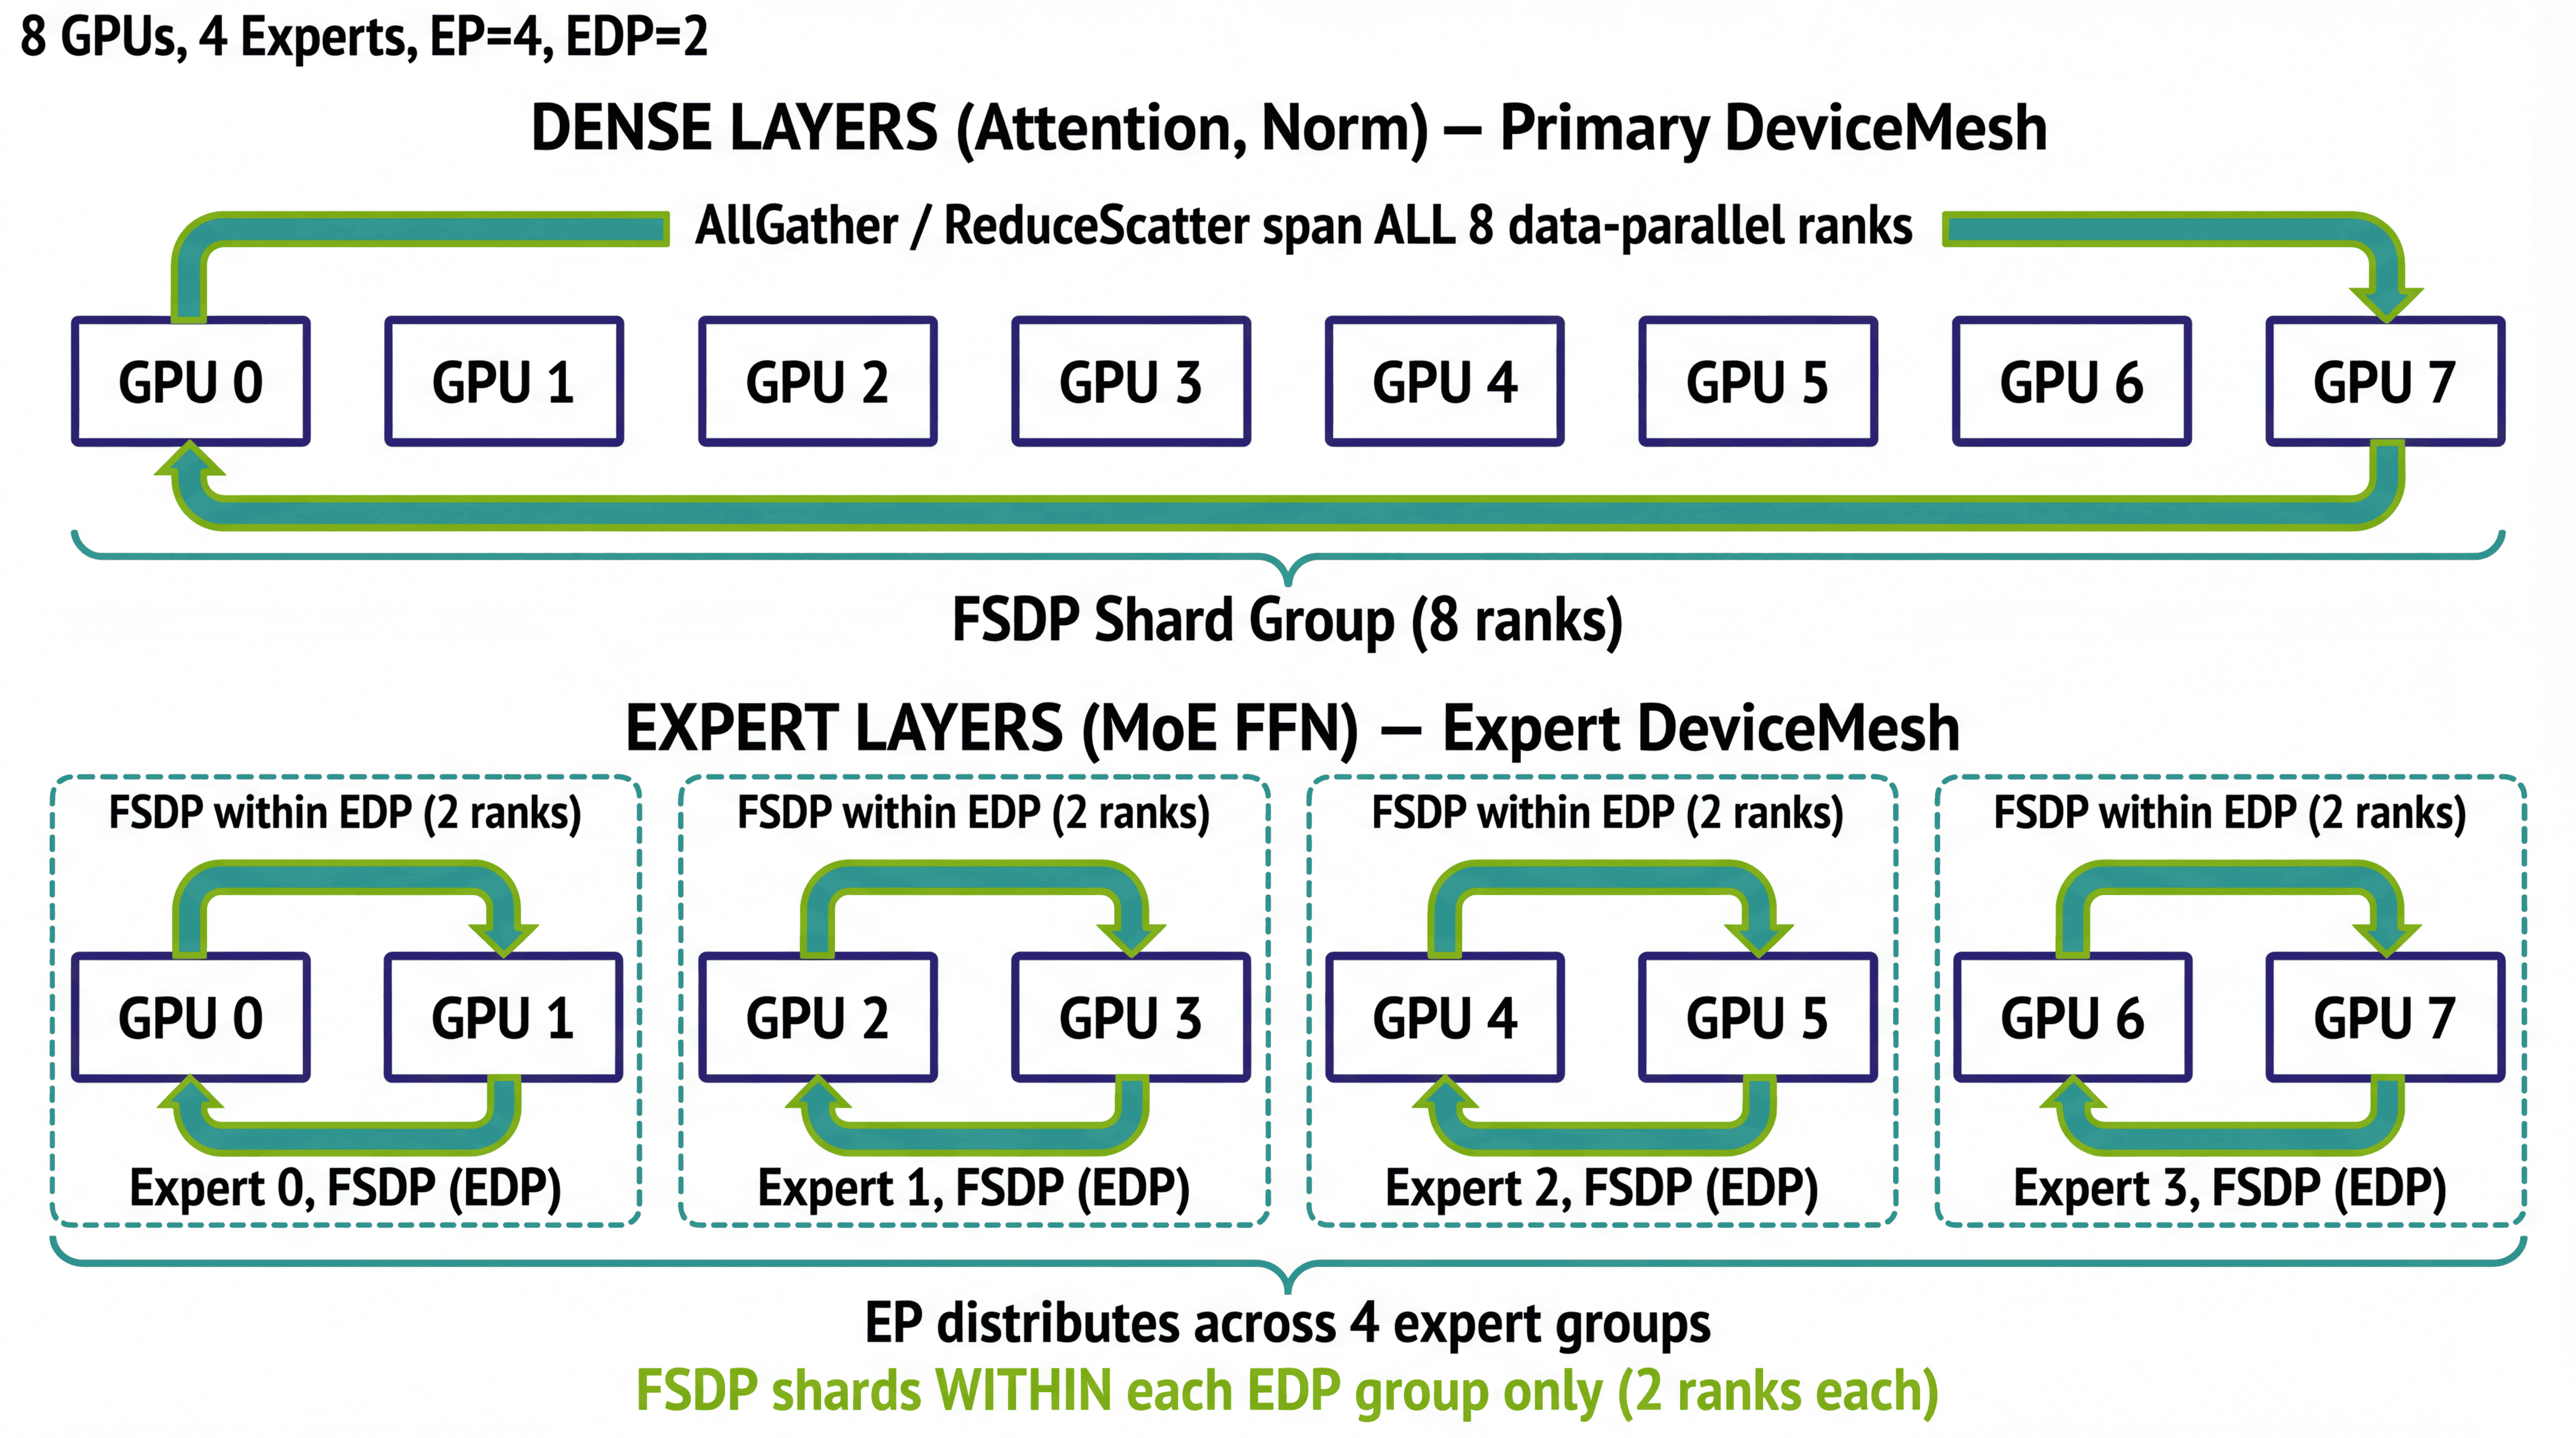
\includegraphics[width=0.95\textwidth]{figures/ai_gen/ai_gen_fsdp_ep_dual_devicemesh.png}
%     \caption{Dual DeviceMesh for FSDP+EP: primary mesh for dense layers, expert mesh for MoE layers.}
%     \label{fig:fsdp-ep-mesh}
% \end{figure}

对于大规模部署，此设计扩展到 \emph{混合分片数据并行} (HSDP)，添加外部 DP 复制维度。 HSDP 完全分片排名子集中的参数并跨子集复制，将 AllGather 限制在组内大小。双 DeviceMesh 为专家和非专家参数保留单独的外部 DP 组，利用 NVLink（节点内）和横向扩展互连（节点间）之间的带宽差距。

\paragraph{零拷贝通信}

双 DeviceMesh 确定哪些等级参与每个 FSDP 集体，但集体本身仍然会带来缓冲区管理和数据复制的开销。 Megatron-FSDP 通过两项优化消除了这种开销。

\textbf{1.非均匀分片：} 标准 FSDP2 沿其主维度独立地对每个参数进行分片，产生统一的每参数分片（图~\ref{fig:fsdp2-sharding}）。相反，Megatron-FSDP 会展平并连接模块内的所有参数，然后在设备之间应用非均匀分片（图~\ref{fig:mfsdp-sharding}）。然后，分片边界与通信缓冲区布局对齐，并且集合直接从扁平化存储中读取，无需冗余复制。在 Llama3 405B 训练中，这将通信开销减少了大约 10\%.

\begin{figure}[ht]
  \centering
  \begin{subfigure}[b]{0.45\textwidth}
    \centering
    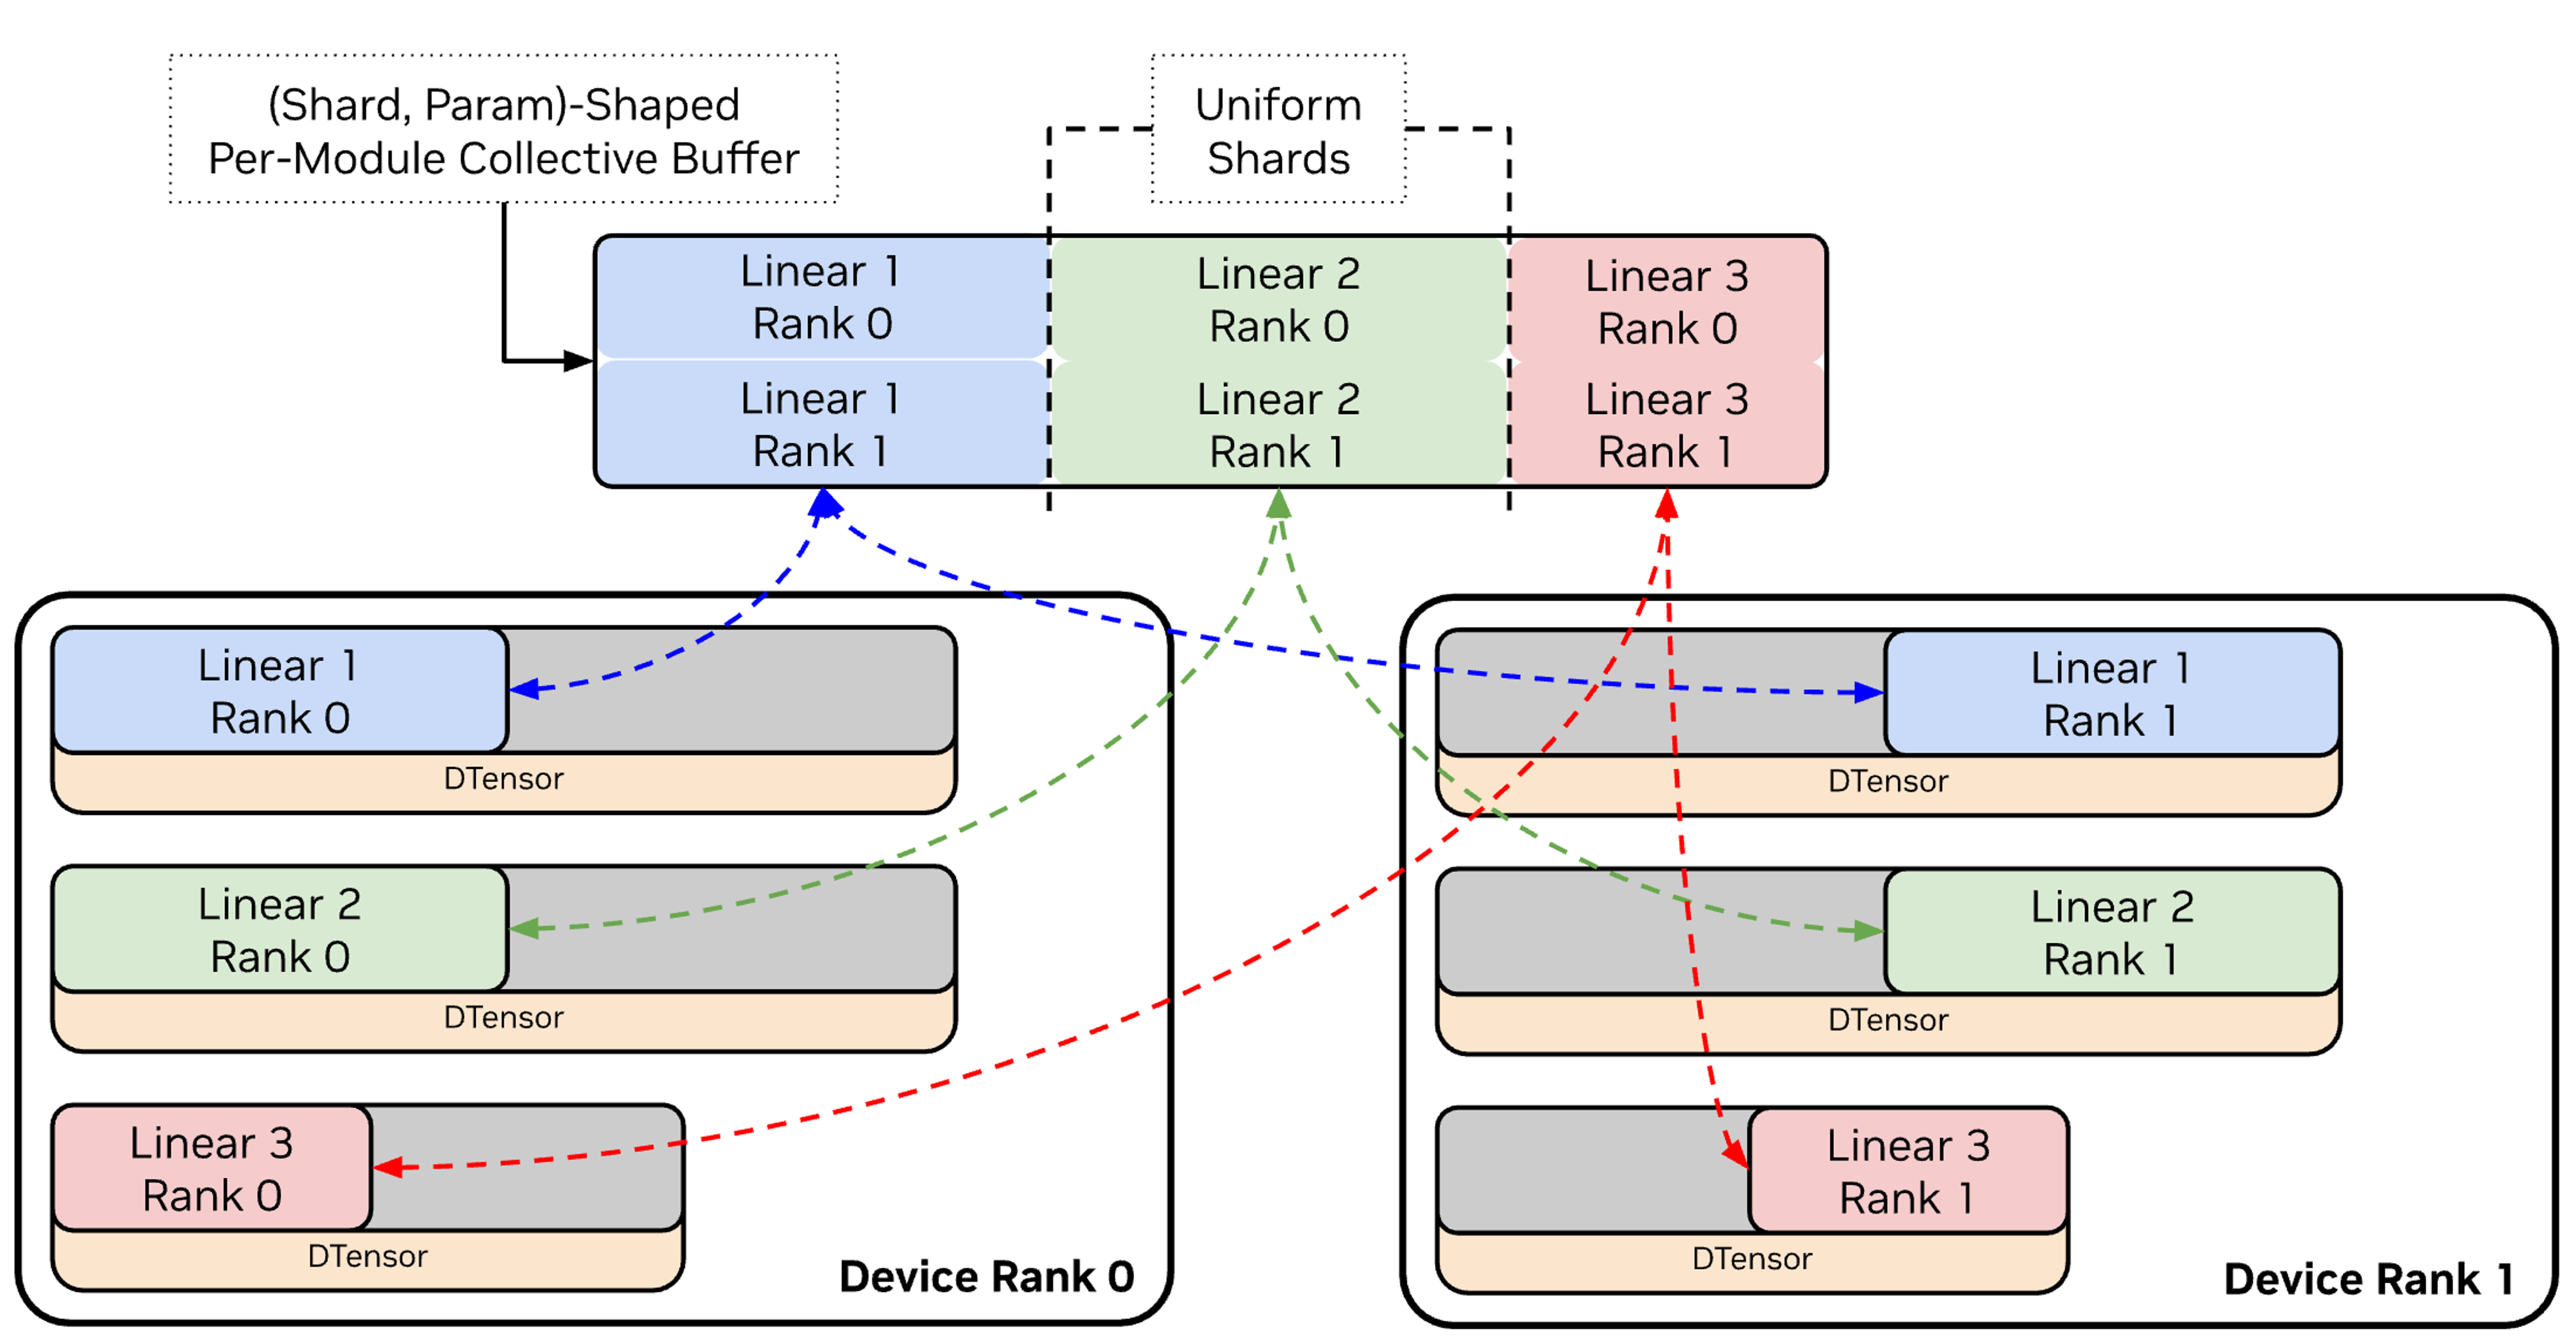
\includegraphics[width=\textwidth]{figures/fsdp2_per_parameter_uniform_sharding.png}
    \caption{FSDP2 按参数均匀分片。}
    \label{fig:fsdp2-sharding}
  \end{subfigure}
  \hfill
  \begin{subfigure}[b]{0.45\textwidth}
    \centering
    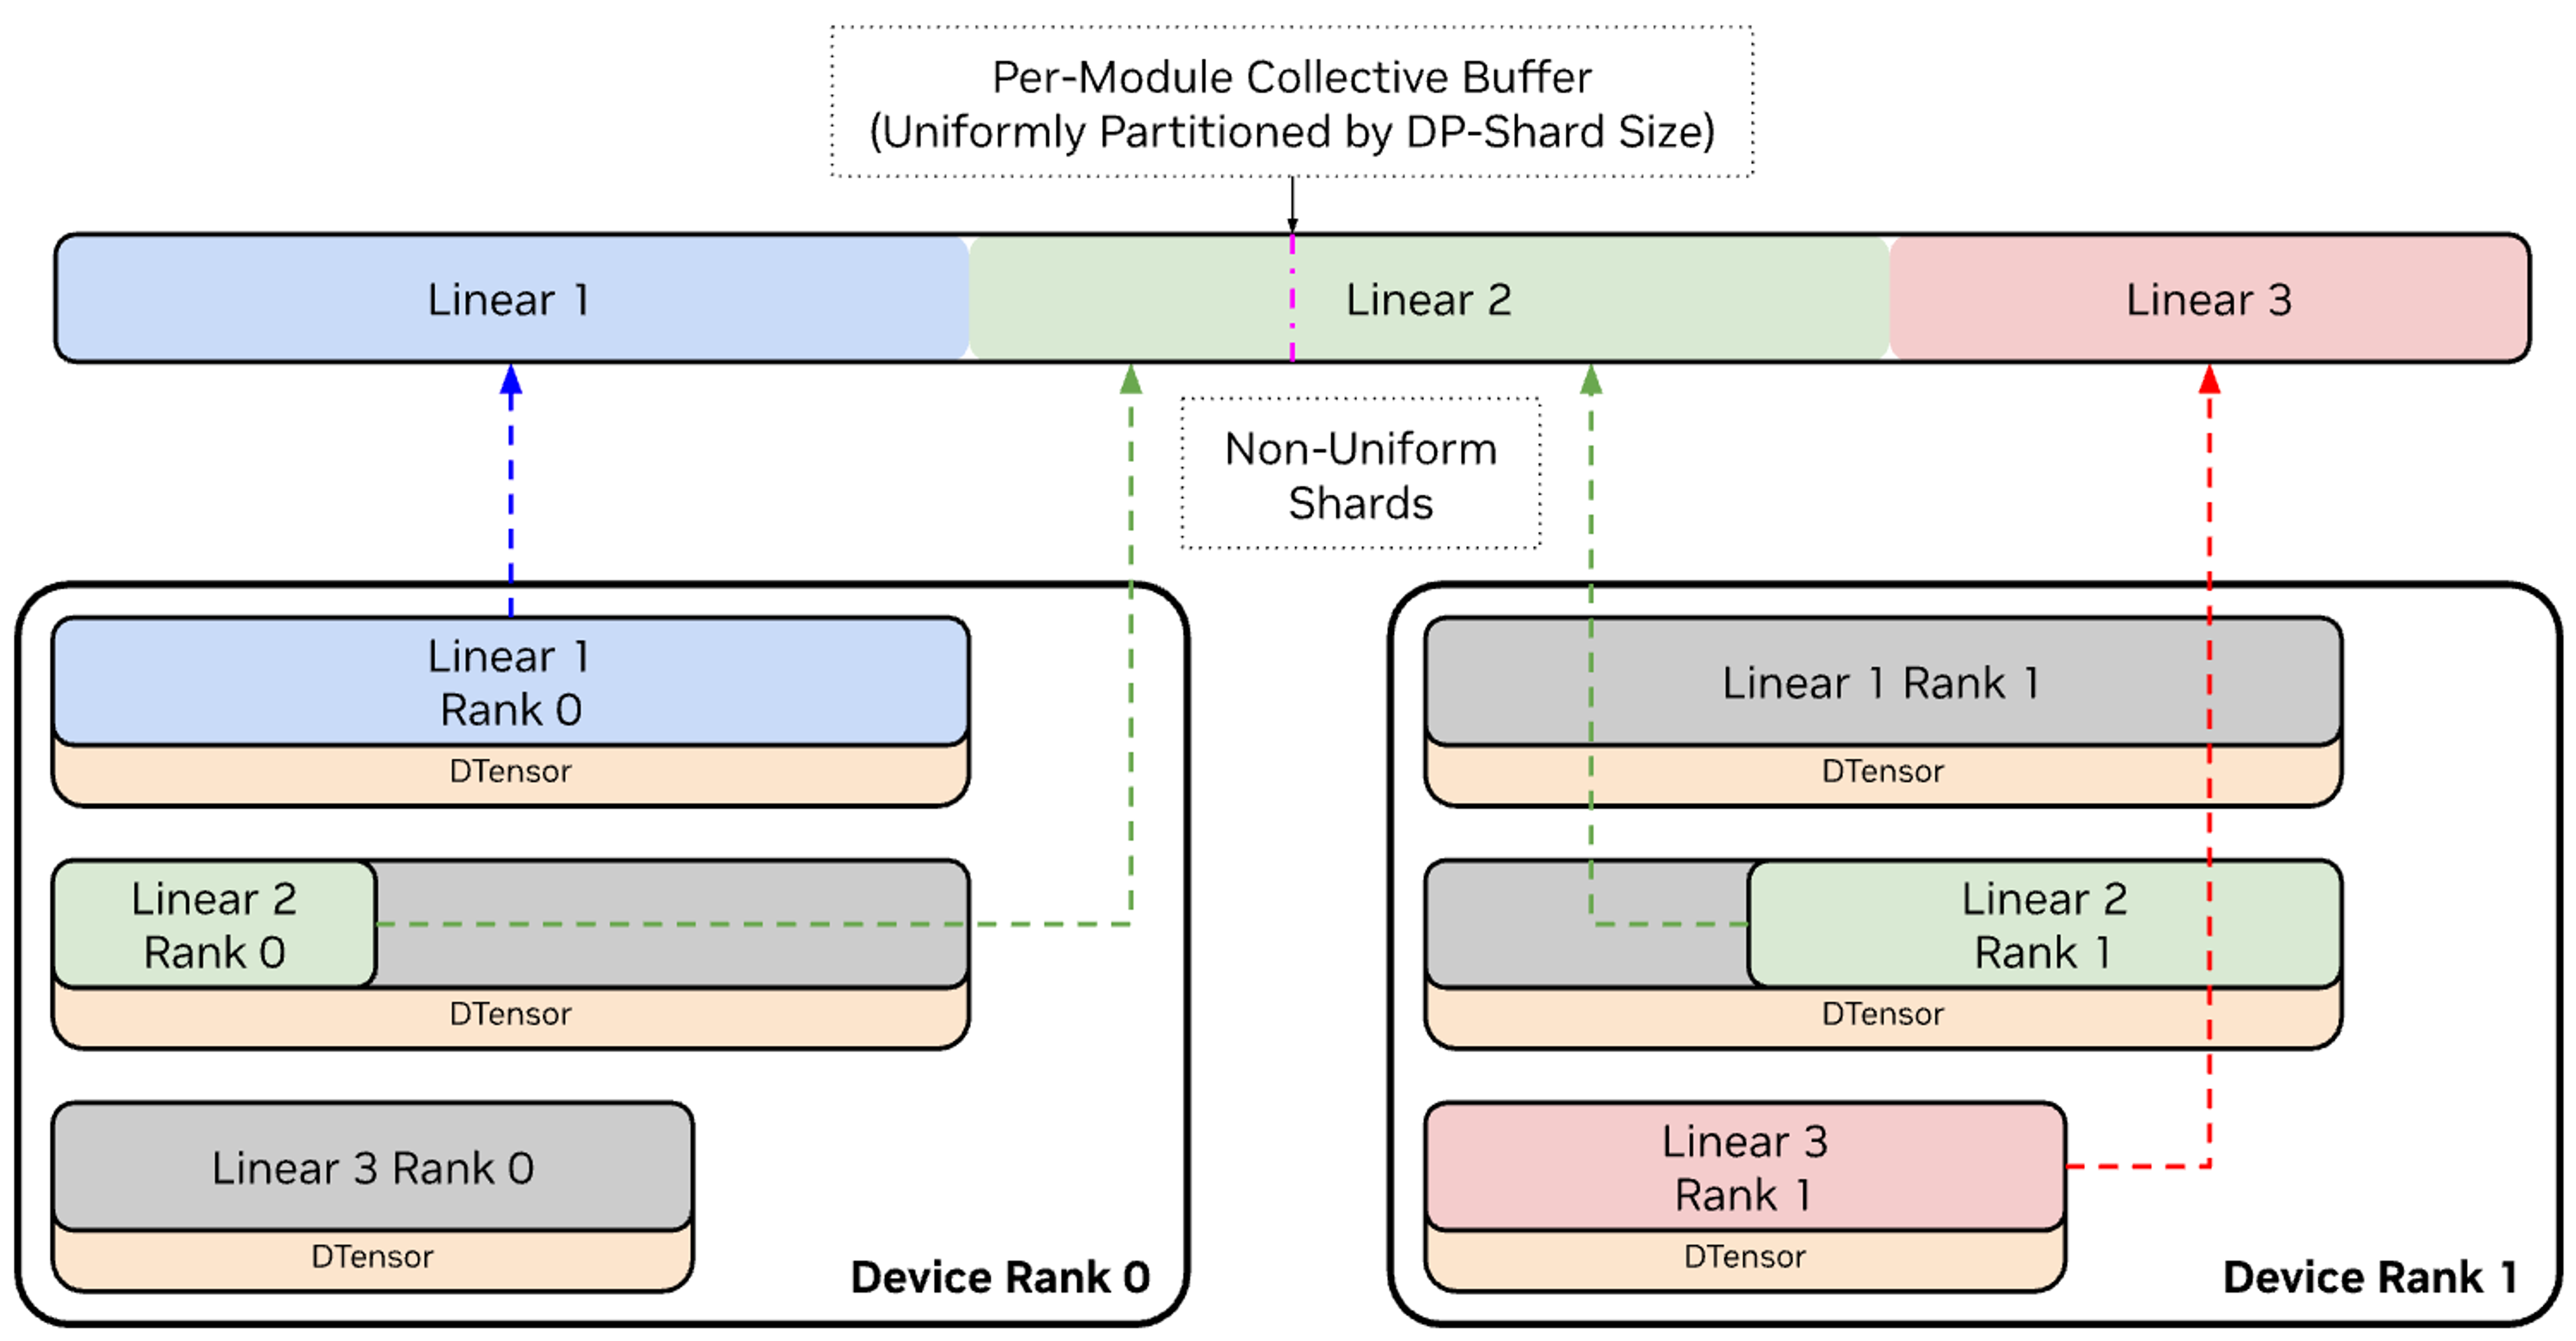
\includegraphics[width=\textwidth]{figures/mfsdp_per_module_non_uniform_sharding.png}
    \caption{Megatron-FSDP 每模块非均匀分片。}
    \label{fig:mfsdp-sharding}
  \end{subfigure}
  \caption{分片策略比较：(a)~FSDP2对各个参数进行统一分片； (b)~Megatron-FSDP 不均匀地展平每个模块和分片，与通信缓冲区对齐。}
  \label{fig:sharding-comparison}
\end{figure}

\textbf{2. 具有 NCCL 用户缓冲区注册的持久双缓冲区：} 基线 FSDP 频繁分配和释放通信缓冲区，NCCL 在每个集合上的用户缓冲区及其内部暂存区域之间复制数据。 Megatron-FSDP 在训练开始时预分配两个持久缓冲区并在它们之间循环（图~\ref{fig:double-buffer}），消除分配流失。 Megatron-FSDP 然后通过用户缓冲区注册 (UBR) 将这些缓冲区注册到 NCCL，因此 NCCL 可以直接读取和写入预先注册的内存，而无需中间副本。综合效果是真正的零拷贝通信。在 NVLink 系统上，通信内核的 SM 占用量从 8--32 个 SM 下降到 1--4 个 SM。在支持 SHARP 的 InfiniBand 上，网络交换机可以完全处理缩减并释放 GPU SM。

\begin{figure}[ht]
  \centering
  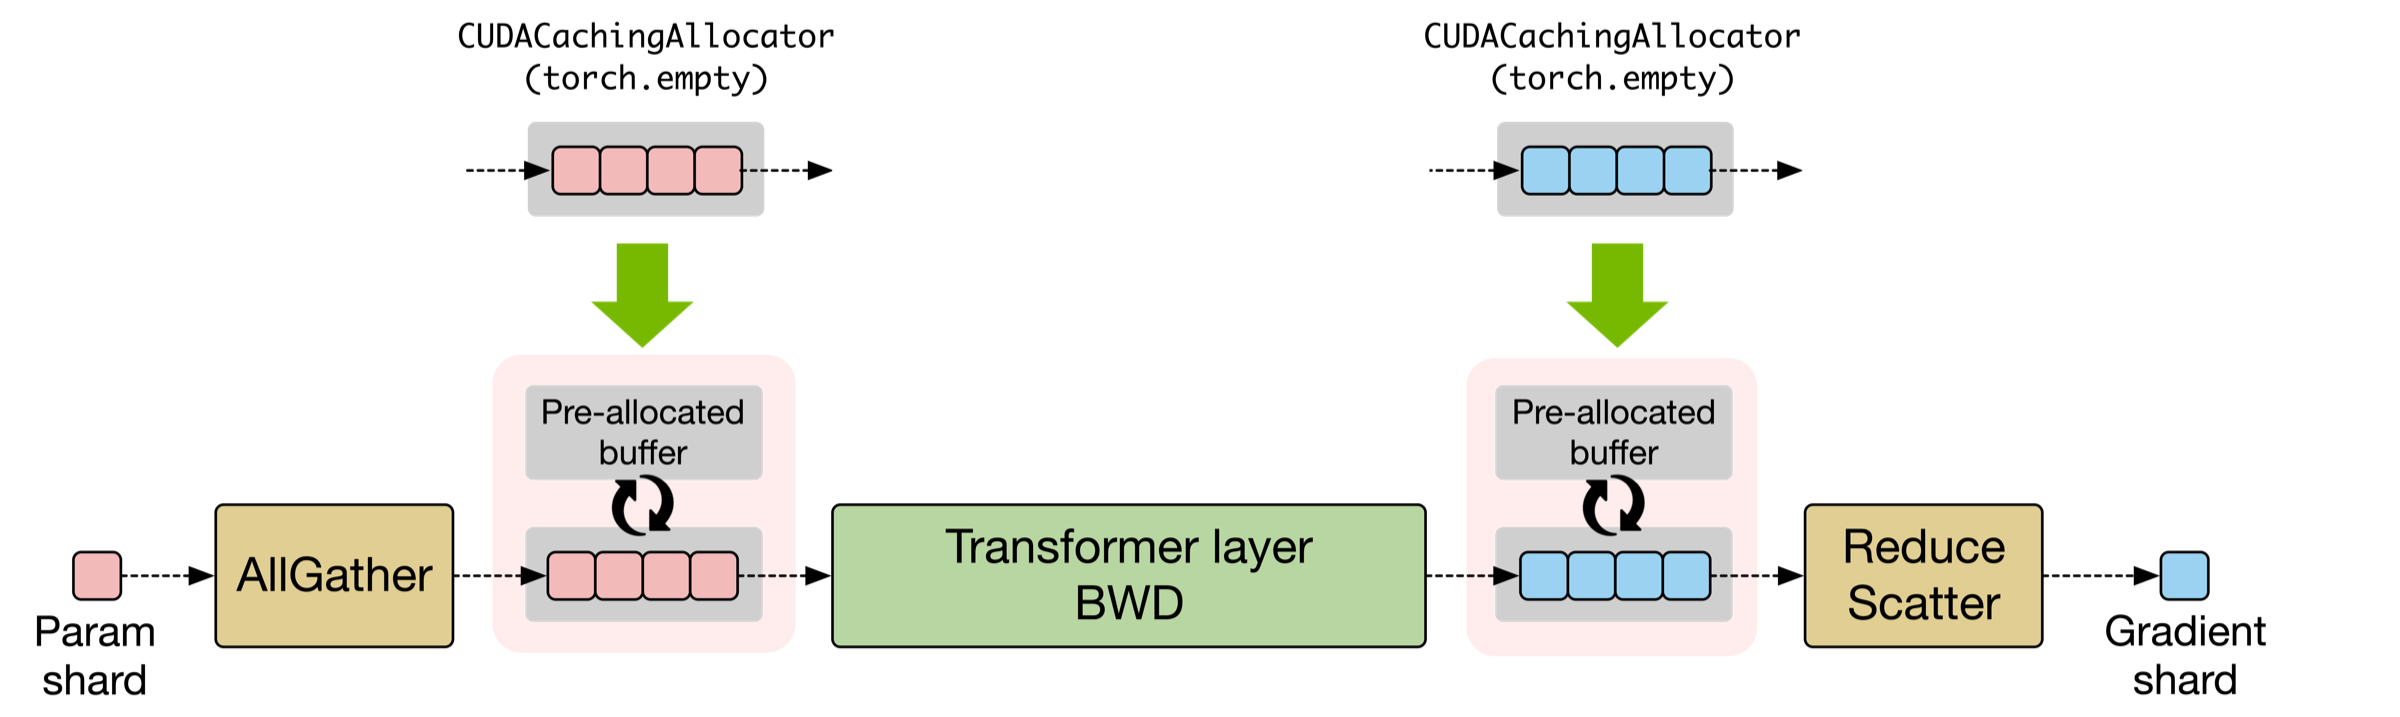
\includegraphics[width=0.85\textwidth]{figures/persistent_double_buffers.png}
  \caption{持久双缓冲区设计：两个预分配缓冲区在 FSDP 集合之间循环，消除了分配开销并启用 NCCL 用户缓冲区注册。}
  \label{fig:double-buffer}
\end{figure}

\paragraph{计算--通信重叠}

即使使用零拷贝集合，AllGather 和ReduceScatter 仍然占用网络，同时GPU 等待参数或梯度同步。 Megatron-FSDP 使用专用 CUDA 流通过计算来管道化这些集合：在当前单元的前向或后向传递仍在执行时发出下一个 FSDP 单元的 AllGather，并且用于梯度的 ReduceScatter 与后续层的后向传递同时运行。增加微批量大小可以扩展可用于隐藏通信的计算窗口，但代价是更高的内存使用量。用户可以通过以下方式调整这种权衡 \texttt{overlap\_param\_gather} 和 \texttt{overlap\_grad\_reduce} 旗帜。

% \paragraph{DTensor-Based Checkpointing}

% Megatron-FSDP represents all model parameters as PyTorch DTensor objects, each carrying a DeviceMesh and Placement that encode its sharding layout. Dense parameters reference the primary DeviceMesh and expert parameters reference the Expert DeviceMesh, so the dual-mesh separation is preserved at the checkpoint level. Checkpointing uses PyTorch's Distributed Checkpoint (DCP) API end-to-end, with no intermediate format conversions. Because DTensor can also express traditional 3D-parallel (TP+PP+DP) layouts, Megatron-FSDP ships conversion tools that translate existing 3D-parallel checkpoints into DTensor-based formats with no manual resharding.

% Summary of memory optimizations
\subsubsection{概括}
表~\ref{tab:memory-opt-summary} 总结了本节中描述的内存优化技术及其主要目标。

\begin{table}[ht]
\centering
\caption{内存优化技术总结。}
\label{tab:memory-opt-summary}
\begin{tabular}{lll}
\toprule
\textbf{技术} & \textbf{内存目标} & \textbf{权衡} \\
\midrule
降低精度训练 & 激活 & 数值精度和 CPU 开销 \\
内存高效排列 & 激活 & - \\
细粒度重新计算 & 激活 & 计算开销 \\
细粒度卸载 & 激活 & CPU 开销和非重叠副本 \\
精度感知优化器 & 优化器状态 & 数值精度 \\
FSDP（含 EP） & 参数+优化器 & 通信开销 \\
\bottomrule
\end{tabular}
\end{table}

这些内存优化相辅相成：内存高效排列以零开销消除冗余存储； FP8/FP4 激活会降低精度，同时对质量影响最小；细粒度重新计算为特定模块提供了有利的计算内存权衡；当其他技术不足时，激活卸载可提供额外的空间；低精度存储和状态卸载减轻了重量并优化了内存； FSDP 可以扩展至超出单设备容量。它们共同将内存从阻塞屏障减少为可管理的约束。

内存优化并不是一个一次性的门，一旦通过就可能被遗忘。对于大规模 MoE 模型，内存在整个优化生命周期中一直是稀缺资源。除了使训练能够继续进行之外，内存空间还可以解锁其他优化：更大的批量大小提供更多的计算来隐藏通信延迟（第~\ref{sec:comm-overlap}），CUDA Graphs需要额外的静态缓冲区（第~\ref{sec:cuda-graphs}），并且 EP 通信重叠必须同时保持多个微批次的激活。以下各节中描述的许多优化都会消耗内存，而上述技术使这种消耗变得可行。

\subsection{打破通信壁垒}\label{sec:comm-wall}

通信开销直接降低了 GPU 利用率：在集体操作中花费的每一微秒都意味着计算能力的损失。优化前，EP全对全通信通常消耗20--60\% 训练时间，取决于模型配置、EP 大小和硬件拓扑。当 EP 位于 NVLink 域内时（例如 GB200 NVL72 上带有 EP64 的 DeepSeek-V3），开销约为 20\%;当EP跨节点边界时（例如跨节点H100上带有EP64的DeepSeek-V3），它上升到40--60\%。本节中的技术针对该频谱上的所有点。

专家并行 (EP) 将专家分布在设备之间，以将 MoE 模型扩展至超出单设备容量，但这种分布引入了独特的通信模式。与 AllReduce 的体积与并行度无关不同，all-to-all 的体积与 token 数量和隐藏维度成正比，并且更大的 EP 推动这种通信跨节点，而带宽有限。对于像 DeepSeek-V3 和 Kimi-K2 这样的细粒度 MoE 架构，三个因素加剧了这一挑战：

\begin{itemize}
    \item \textbf{高频}：更多的专家意味着每层有更多的调度/组合操作（DeepSeek-V3 有 58 个 MoE 层，每个层需要两次 all-to-all 操作）。
    \item \textbf{跨节点瓶颈}：对于跨越多个节点的大 EP，由于带宽较低，节点间的所有到所有延迟占主导地位。
    \item \textbf{算术强度低}：小专家可以快速完成计算，从而减少与通信重叠的时间。
\end{itemize}

\subsubsection{通信剖析：专家并行模式}

\begin{figure}[ht]
    \centering
    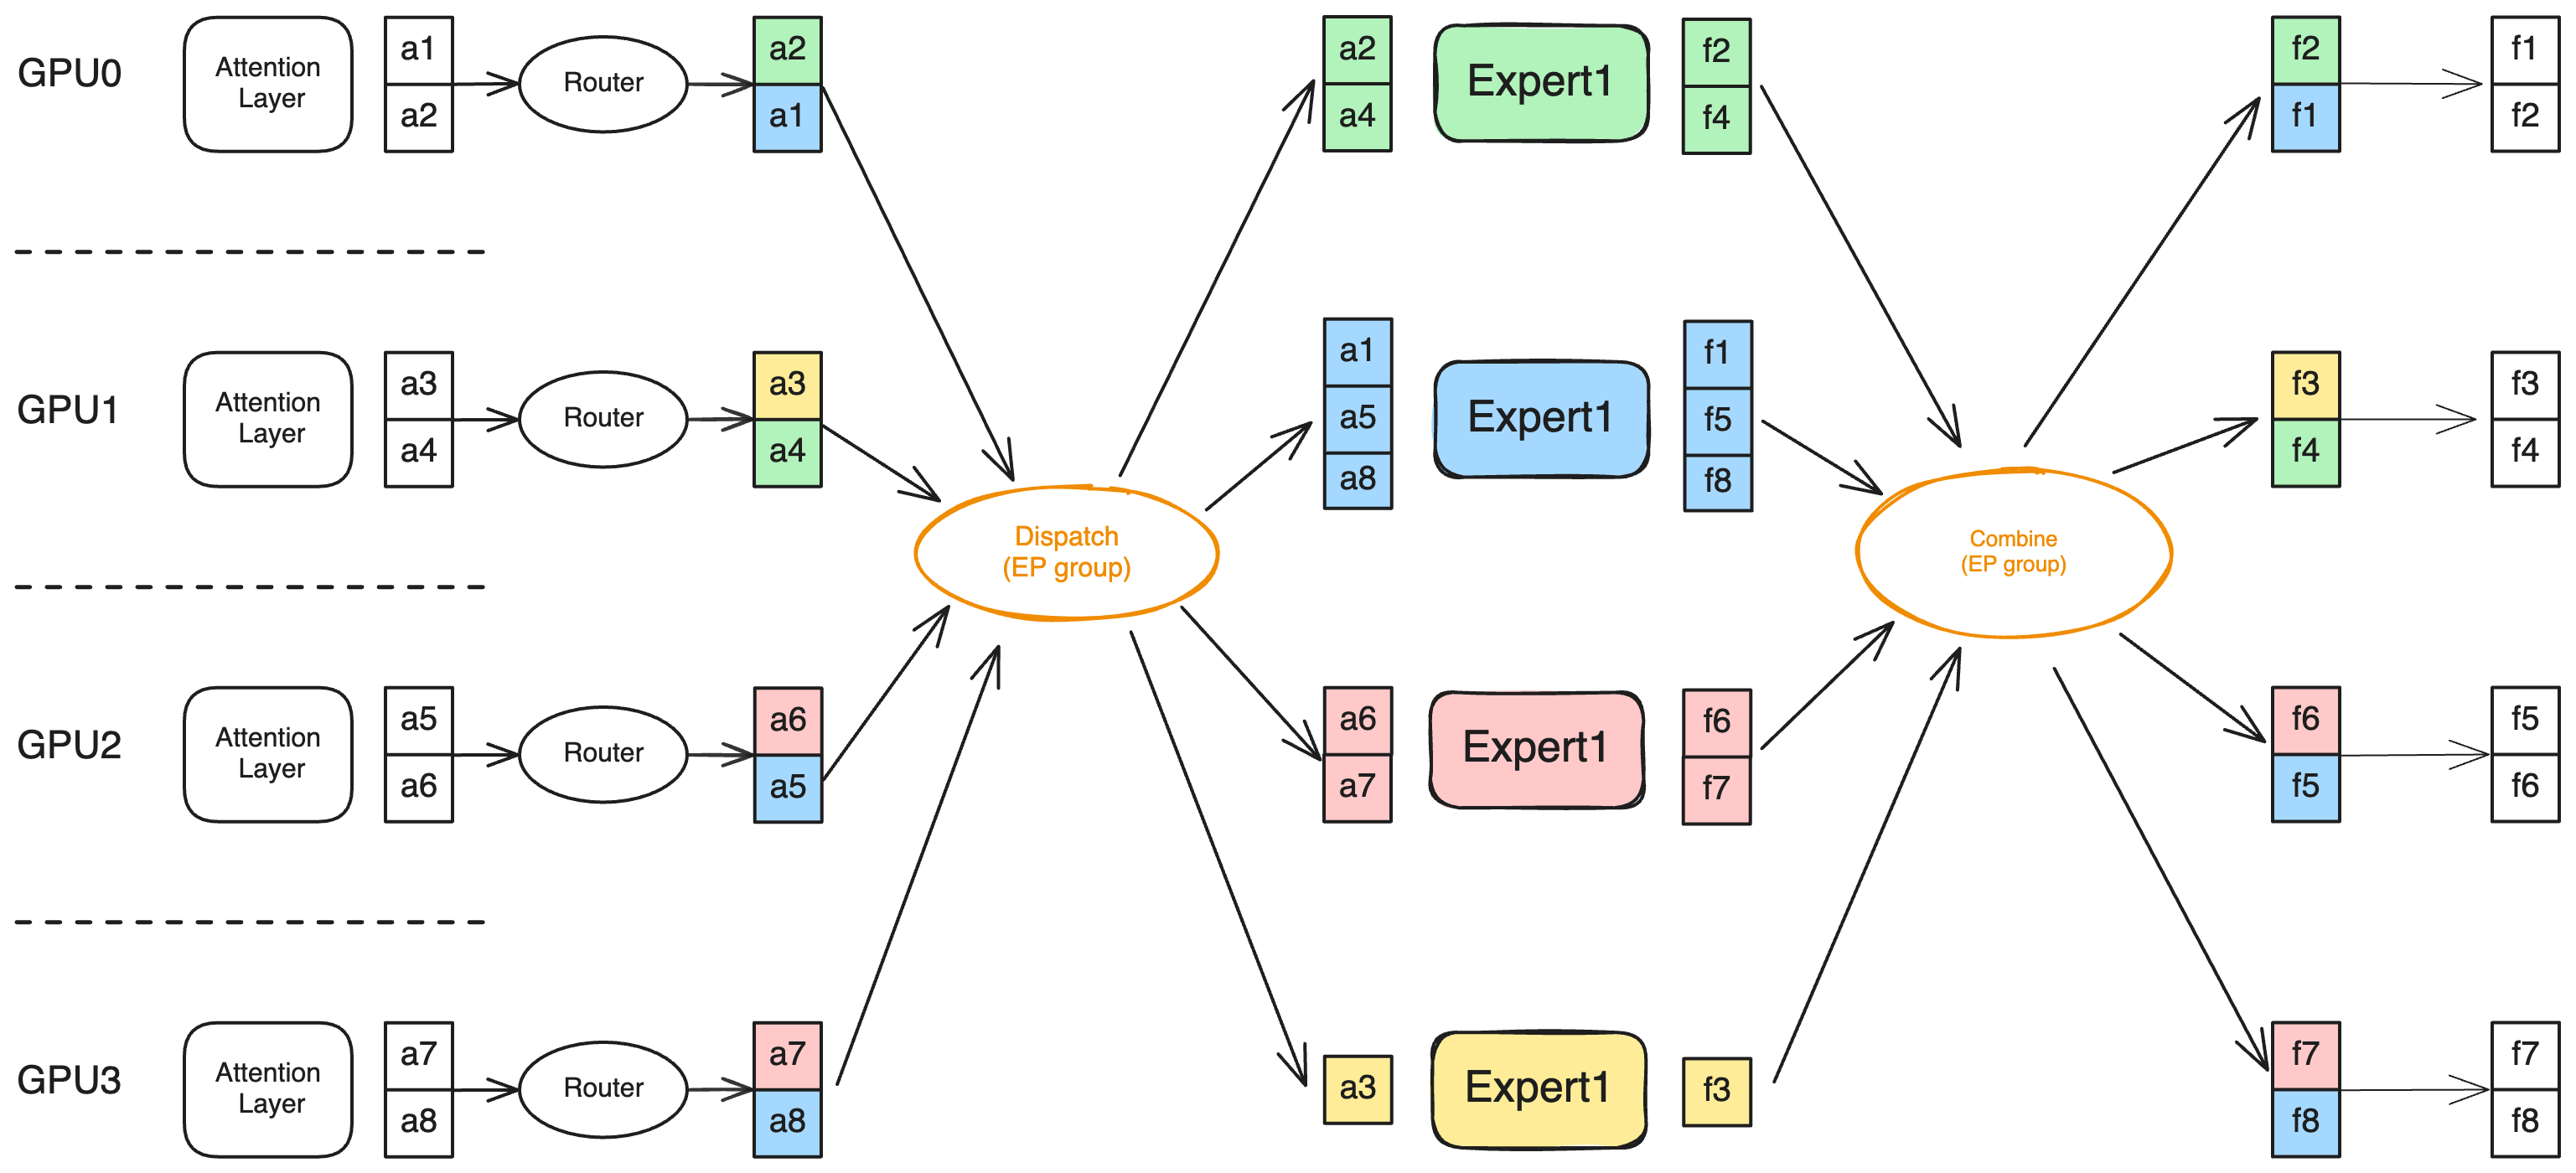
\includegraphics[width=0.8\linewidth]{figures/EP_comm.png}
    \caption{跨 4 个 GPU 和 4 个专家的专家并行。}
    \label{fig:EP_comm}
\end{figure}

\Figref{fig:EP_comm} 说明了专家并行通信模式。在标准 EP 实现中，每个 MoE 层需要两个集体通信操作： \textit{派遣} 将令牌发送给指定的专家，并且 \textit{结合} 将处理后的令牌返回到其原始排名。对于具有 $L$ MoE 层， $B$ 每批次的标记，隐藏维度 $h$，和 EP 学位 $\text{EP}$，每次前向传播涉及 $2L$ 调度/合并操作，每次传输 $O(Bh)$ 数据跨 $\text{EP}$ 行列。

在 DeepSeek-V3 规模下，这相当于 58 个 MoE 层 $\times$ 2 个操作/层 = 每个前向传递 116 个调度/组合操作。向后传递使该计数加倍。在 50 GB/s 节点间带宽（例如 InfiniBand NDR）下，具有 200 MB 有效负载的单次调度需要几毫秒，每次迭代累积到数百或数千毫秒。

通信量由EP配置决定，在不改变并行策略的情况下无法减少通信量。因此，优化必须针对通信的执行和调度方式。两种策略协同作用来解决通信开销：

\begin{enumerate}
    \item \textbf{最大化带宽利用率。} 标准 NCCL 全面实施并未充分利用可用带宽，特别是对于细粒度的 MoE 工作负载。优化调度程序（DeepEP、HybridEP）使用专门的内核来融合操作并利用硬件原语来接近峰值带宽。
    \item \textbf{将延迟隐藏在计算背后。} 即使具有最佳带宽，全面操作也需要时间。通过将通信与相邻微批次的计算重叠，可以隐藏该延迟，而不是暴露在关键路径上。
\end{enumerate}

以下小节介绍了按这些策略组织的技术：带宽优化（DeepEP、HybridEP）和延迟隐藏（EP 通信重叠、管道集成）。

\subsubsection{DeepEP 和 HybridEP：最大化 EP 带宽}\label{sec:deepep}

在传统的 EP 实现中，令牌交换依赖于所有人对所有人的通信。即使使用优化的 NCCL 集体，这条路径也有固有的局限性：在调度之前需要一个排列阶段，它复制每个令牌顶部 -$k$ 次并产生冗余流量。在某些设置中，此预处理也会表现为主机开销。

为了解决这些问题，Megatron-Core 提供了两个基于令牌的调度后端：HybridEP 和 DeepEP \cite{deepep2025}。基于令牌的调度消除了排列步骤并避免发送冗余令牌，从而减少总体通信量并提高有效带宽。

HybridEP 由 NVIDIA 开发。它遵循与 DeepEP 相同的基于令牌的原则，利用 TMA 和 IBGDA 等硬件原语，并以较低的 SM 使用率实现相当或更高的带宽，包括多节点 NVLink (MNVL) 部署。


\begin{figure}[ht]
    \centering
    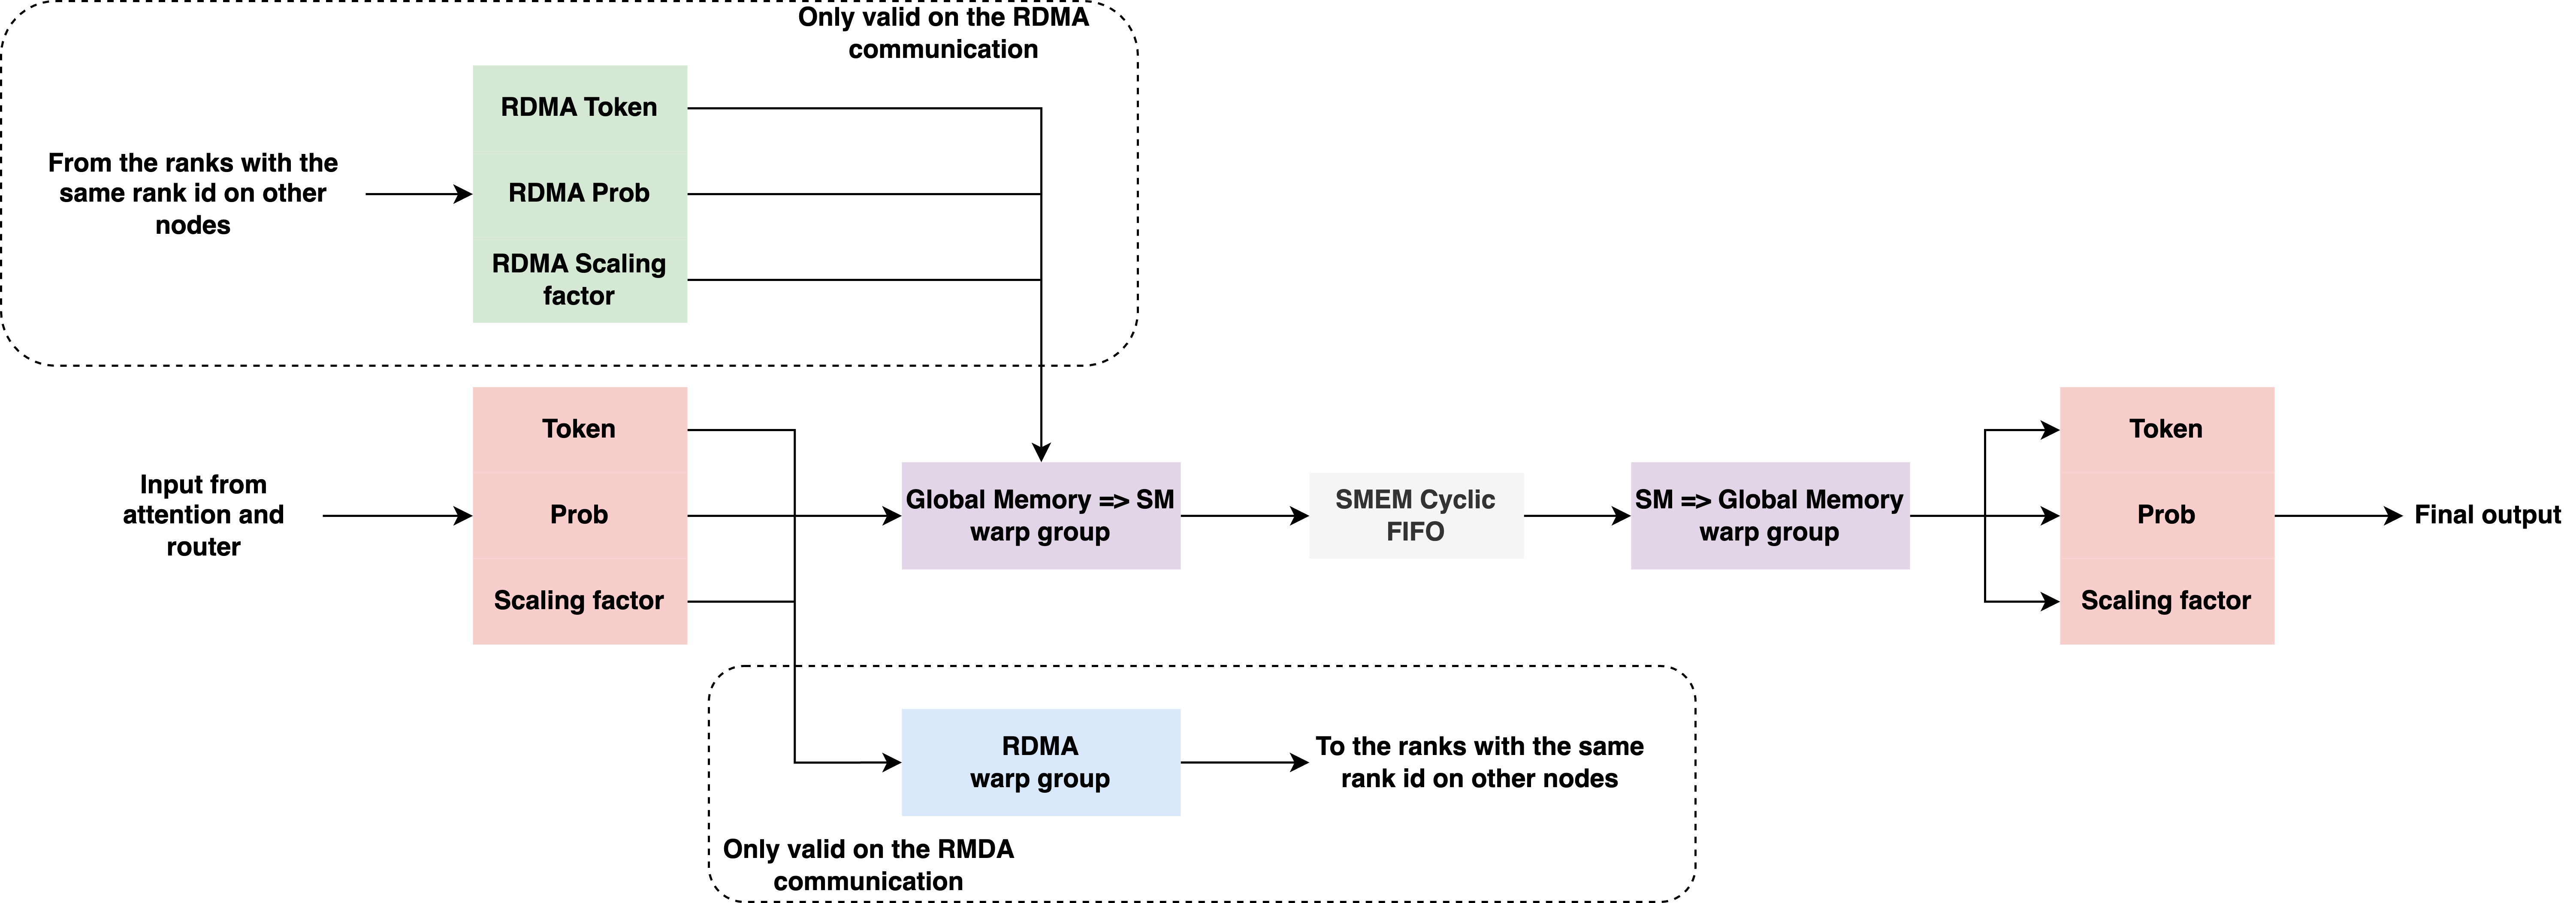
\includegraphics[width=1\linewidth]{figures/hybrid_ep_dispatch.drawio.png}
    \caption{HybridEP的调度内核设计。}
    \label{fig:hybrid_ep_dispatch}
\end{figure}

对于调度，如图所示 \figref{fig:hybrid_ep_dispatch}，HybridEP根据路由信息从全局内存读取数据到共享内存中，然后通过FIFO队列将令牌写入目的地。在节点间的情况下，HybridEP 不是直接通过网络接口发送重复的有效负载，而是首先使用 RDMA 扭曲组在跨节点具有相同本地索引的 GPU 之间交换数据，然后在每个节点内转发。这减少了跨节点流量并允许节点间和节点内传输重叠。

\begin{figure}[ht]
    \centering
    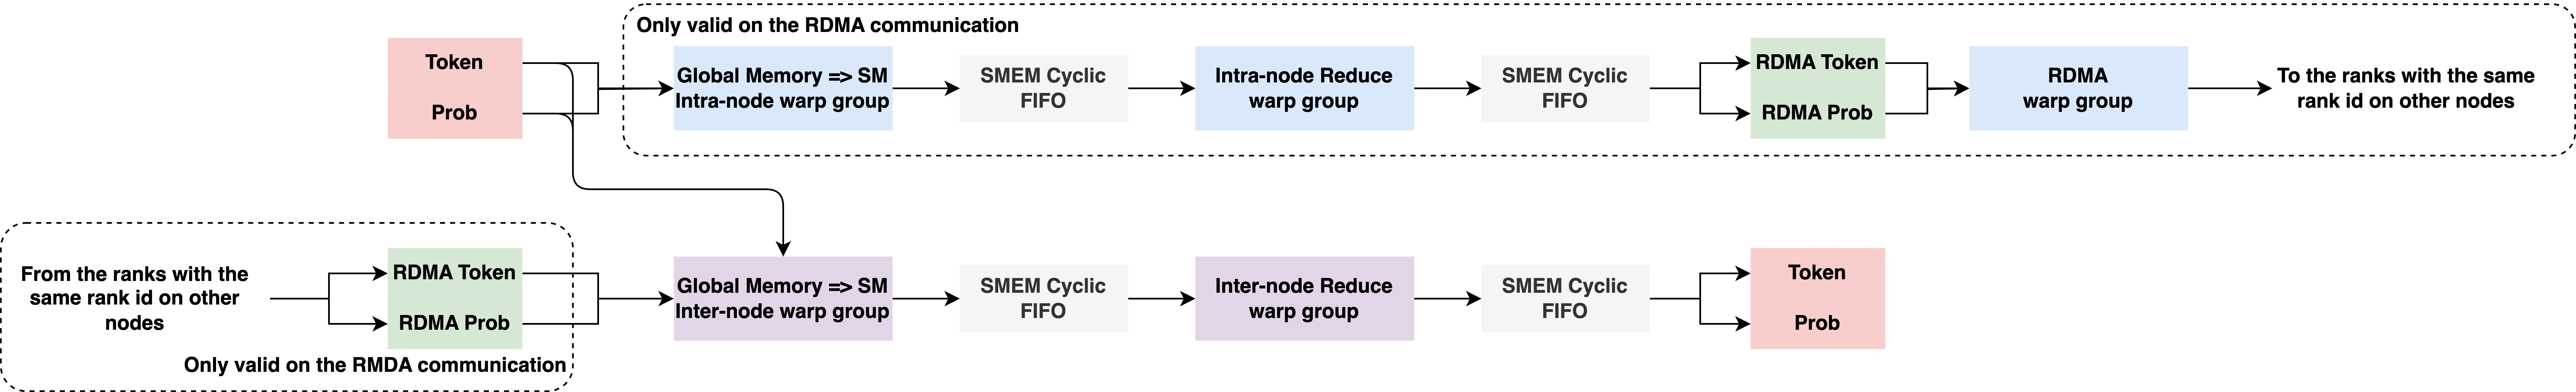
\includegraphics[width=1\linewidth]{figures/hybrid_ep_combine.drawio.png}
    \caption{HybridEP的组合内核设计。}
    \label{fig:hybrid_ep_combine}
\end{figure}

对于组合，标准的全对全调度仅执行通信，因此之后需要单独的取消排列阶段。相反，HybridEP 将缩减融合到通信内核中。如图所示 \figref{fig:hybrid_ep_combine}，HybridEP通过FIFO队列读取数据，执行归约，并将结果直接写入目标位置。在节点间设置中，HybridEP 首先对必须跨节点通信的数据进行跨节点归约，然后在每个节点内完成第二次归约。


我们在 GB200 和 H100 上评估全对全调度和 HybridEP，隐藏大小为 7168，序列长度为 4096，多个 EP 大小下有 256 个专家。结果总结在表中~\ref{tab:hybrid-ep}。在所有测试设置中，HybridEP 始终优于所有设置，在节点间场景中获得更大收益。该表仅报告通信延迟；在端到端训练中，一旦包含排列和主机开销，差距通常会更大。

\begin{table}[ht]
\centering
\caption{HybridEP 和 all-to-all 的 EP 扩展性能（以 $\mu$s 为单位）。}
\label{tab:hybrid-ep}
\begin{tabular}{llrrrr}
\toprule
 &  & \multicolumn{2}{c}{GB200（微秒）} & \multicolumn{2}{c}{H100（微秒）} \\
 & EP尺寸 & HybridEP & 全部到全部 & HybridEP & 全部到全部 \\
\midrule
\multirow{4}{*}{dispatch}
 & 8  & 391 & 735 & 661  & 1265 \\
 & 16 & 578 & 743 & 1485 & 5774 \\
 & 32 & 612 & 769 & 3064 & 8059 \\
 & 64 & 675 & 930 & 4626 & 9164 \\
\midrule
\multirow{4}{*}{combine}
 & 8  & 353 & 741 & 624  & 1277 \\
 & 16 & 527 & 765 & 1688 & 5628 \\
 & 32 & 646 & 758 & 3088 & 7815 \\
 & 64 & 744 & 827 & 4398 & 8727 \\
\bottomrule
\end{tabular}
\end{table}



\subsubsection{EP 通信重叠：隐藏 EP 通信延迟}\label{sec:comm-overlap}

优化的调度器改善了整体 \textit{带宽利用率}，但根本问题仍然存在：all-to-all 仍然位于端到端的关键路径上。对于带有 EP64 的 DeepSeek-V3，EP 全对全通信仍然可能占到 30--40\% 的迭代时间，直接限制吞吐量。

关键的观察结果是，所有到所有的延迟可以是 \textit{隐} 当重叠窗口中存在足够的独立工作时，落后于计算 \cite{wang2022coconet,wang2024flux}。对于 DeepSeek-V3 和 Kimi-K2 等细粒度 MoE 模型来说，这是一个挑战，因为跨节点 EP 通信可能会消耗大约一半的层时间，而相邻算子（例如 GEMM）通常太短而无法隐藏它。

为了解决这种不平衡问题，Megatron-Core 使用专用的 1F1B 全部重叠方案 \cite{1f1boverlap} 合并来自相邻微批次的前向和后向传递，并跨 CUDA 流交错计算和all-to-all内核 \cite{narayanan2019pipedream,huang2019gpipe}。具体来说，一个微批次的后向all-to-all与另一个微批次的前向注意力/MLP 重叠。从概念上讲，这是一个类似 DualPipe 的 \cite{hfdualpipe} 双向时间表建立在标准 1F1B 之上，同时保留Megatron-Core兼容性。

为了在 1F1B 中实现全部重叠，我们合并相邻的微批量前向和后向传递并评估两种模式：

\begin{enumerate}
    \item \textbf{合并的 FWD-FWD / BWD-BWD}：此策略合并来自两个微批次的相同类型的通道（\figref{fig:fwd_fwd_merge}）。在 \textit{前传-前传}，微批次 0 和 1 的前向传递并行运行，并与计算全部重叠。 \textit{BWD-BWD} 将相同的原理应用于向后传递。这种方法有明显的权衡：
    \begin{itemize}[leftmargin=*]
        \item \textbf{内存开销}：2 倍峰值激活内存。
        \item \textbf{全部到全部重叠}：隐藏 all-to-all 的机会较少，因为前向计算大约是后向计算的一半。
    \end{itemize}
    
    \begin{figure}[ht]
        \centering
        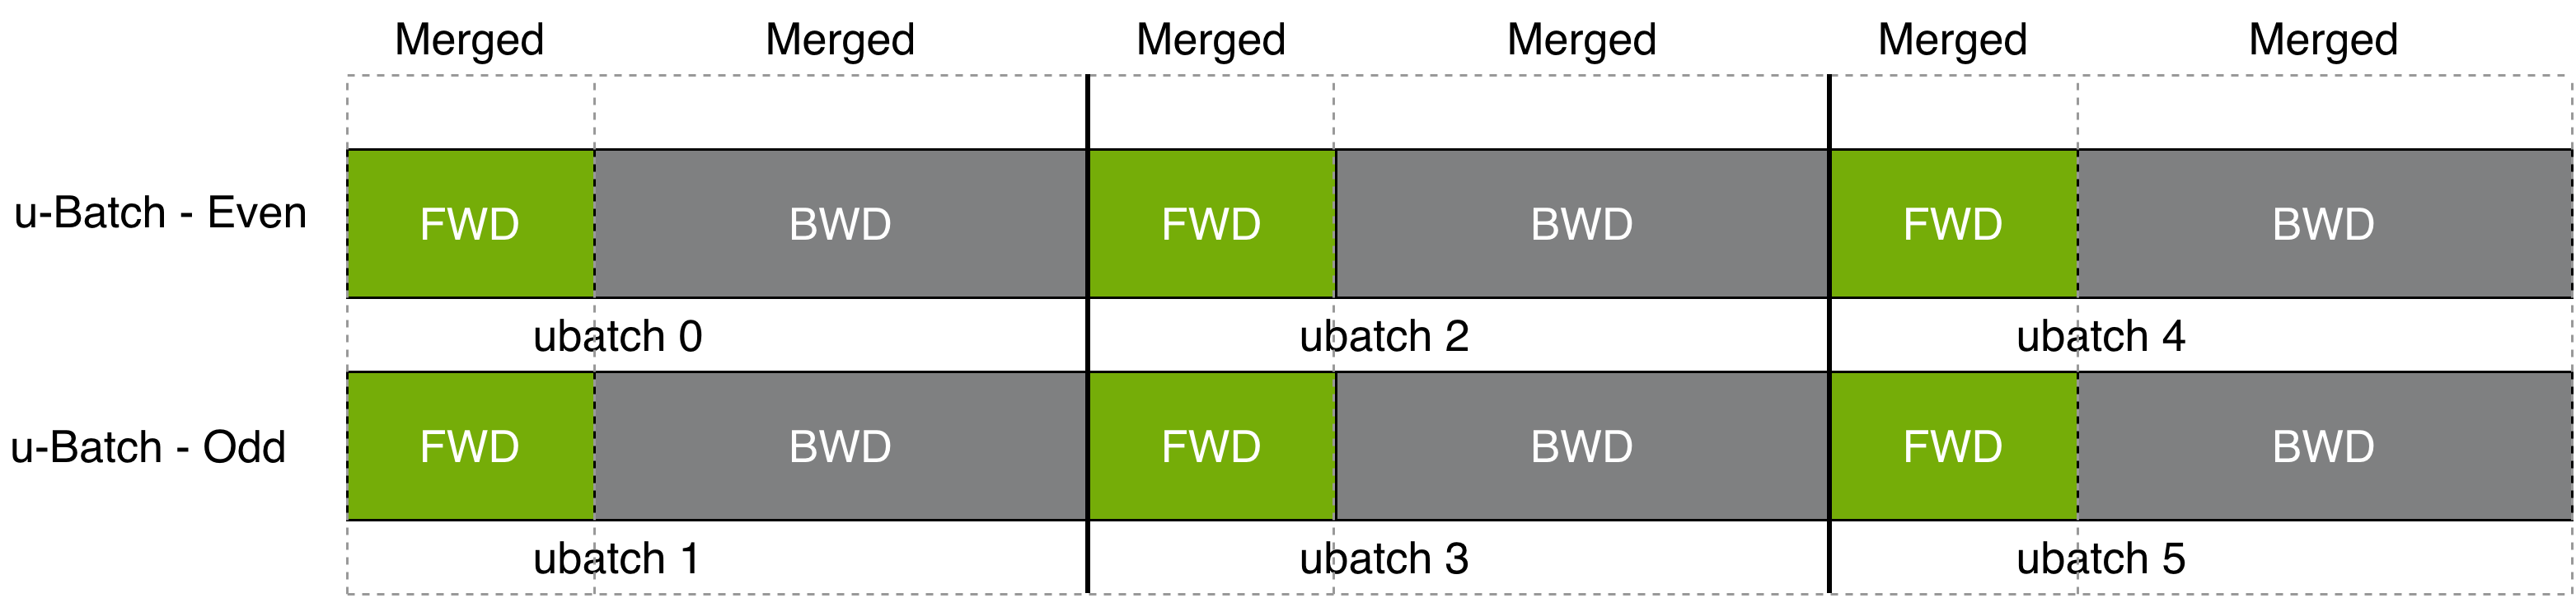
\includegraphics[width=0.8\linewidth]{figures/EP_Overlap_merged_fwd_fwd.png}
        \caption{将 FWD-FWD 时间线与全部重叠合并。}
        \label{fig:fwd_fwd_merge}
    \end{figure}

    \item \textbf{合并的 FWD-BWD（DualPipe 等效）}：这是首选策略（\figref{fig:fwd_bwd_merge}）。它将一个微批次的前向传递与另一个微批次的后向传递合并（例如，微批次 1 的 FWD 与微批次 0 的 BWD）。与相比 \textit{前传-前传}，它提供：
    \begin{itemize}[leftmargin=*]
        \item \textbf{内存开销}：没有额外的内存开销（前向传递中的激活可重复用于后向传递）。
        \item \textbf{兼容性}：匹配 DualPipe 的设计，但避免了复杂的调度。
        \item \textbf{局限性}：第一个FWD和最后一个BWD保留在端到端关键路径上，因此它们的all-to-all不能被隐藏。
    \end{itemize}

    
    \begin{figure}[ht]
        \centering
        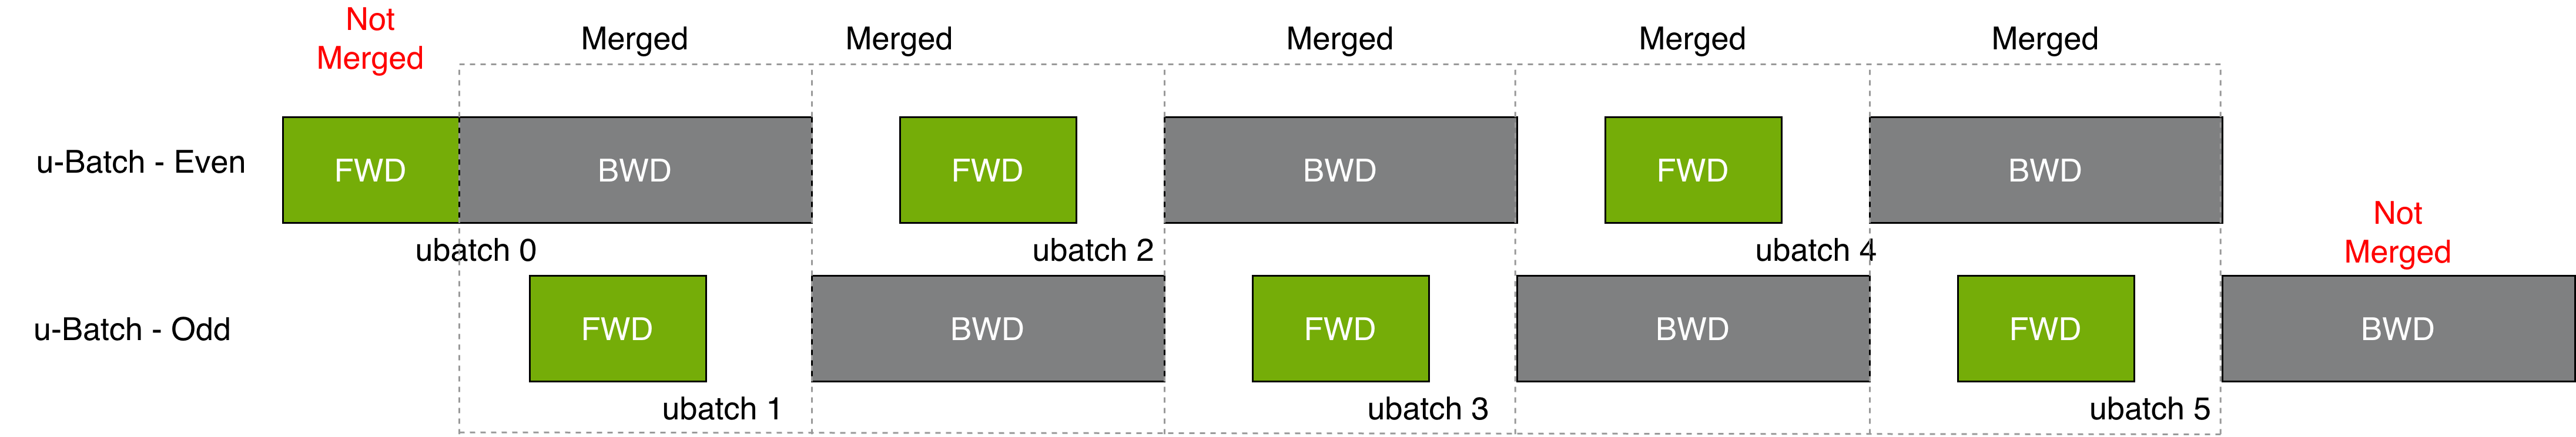
\includegraphics[width=0.8\linewidth]{figures/EP_Overlap_merged_fwd_bwd.png}
        \caption{将 FWD-BWD 时间线与全部重叠合并。}
        \label{fig:fwd_bwd_merge}
    \end{figure}
\end{enumerate}

为了最大化合并的 FWD-BWD 中的全部隐藏，我们使用了两个关键优化：

\begin{enumerate}
    \item \textbf{流分离}：我们将工作负载分成两个 CUDA 流：
    \begin{itemize}[leftmargin=*]
        \item \textit{计算流}：运行前向/后向计算（例如，注意力、专家 MLP）。
        \item \textit{通信流}：运行全对全通信（例如，EP 的令牌调度/组合）。
    \end{itemize}
    通过跨流交替任务，所有到所有的计算与计算并行运行，从而最大限度地减少空闲周期。

    \item \textbf{W/D 分割（权重梯度/数据梯度分割）} \cite{deepseekai2025deepseekv3technicalreport}：一个关键依赖块重叠：向后调度（B/dispatch）需要来自向后 MLP（B/mlp）的输出。为了打破这种依赖性，我们将向后 MLP 拆分为：
    \begin{itemize}[leftmargin=*]
        \item \textit{瓦/MLP}：权重梯度计算（独立于B/dispatch）。
        \item \textit{D/MLP}：数据梯度计算（馈入B/调度）。
    \end{itemize}
    这种分割减少了计算流空闲时间：当 F/mlp 单独太短时，W/mlp 可以与 F/mlp 重叠以隐藏 B/dispatch。
\end{enumerate}
\Figref{fig:ep-all-to-all-overlap} 总结了这些优化。基线（顶部）按顺序执行，其中所有到所有块计算。 1F1B FWD-BWD 方案（底部）交错相邻的微批次，因此通信可以隐藏在计算后面。 W/D 的分裂进一步增加了重叠的机会。这些方法共同减少了 30--40 的 EP 通信开销\% （DeepEP 之后）低于 5\% H100 上 DeepSeek-V3 训练的迭代时间。

\begin{figure}[ht]
    \centering
    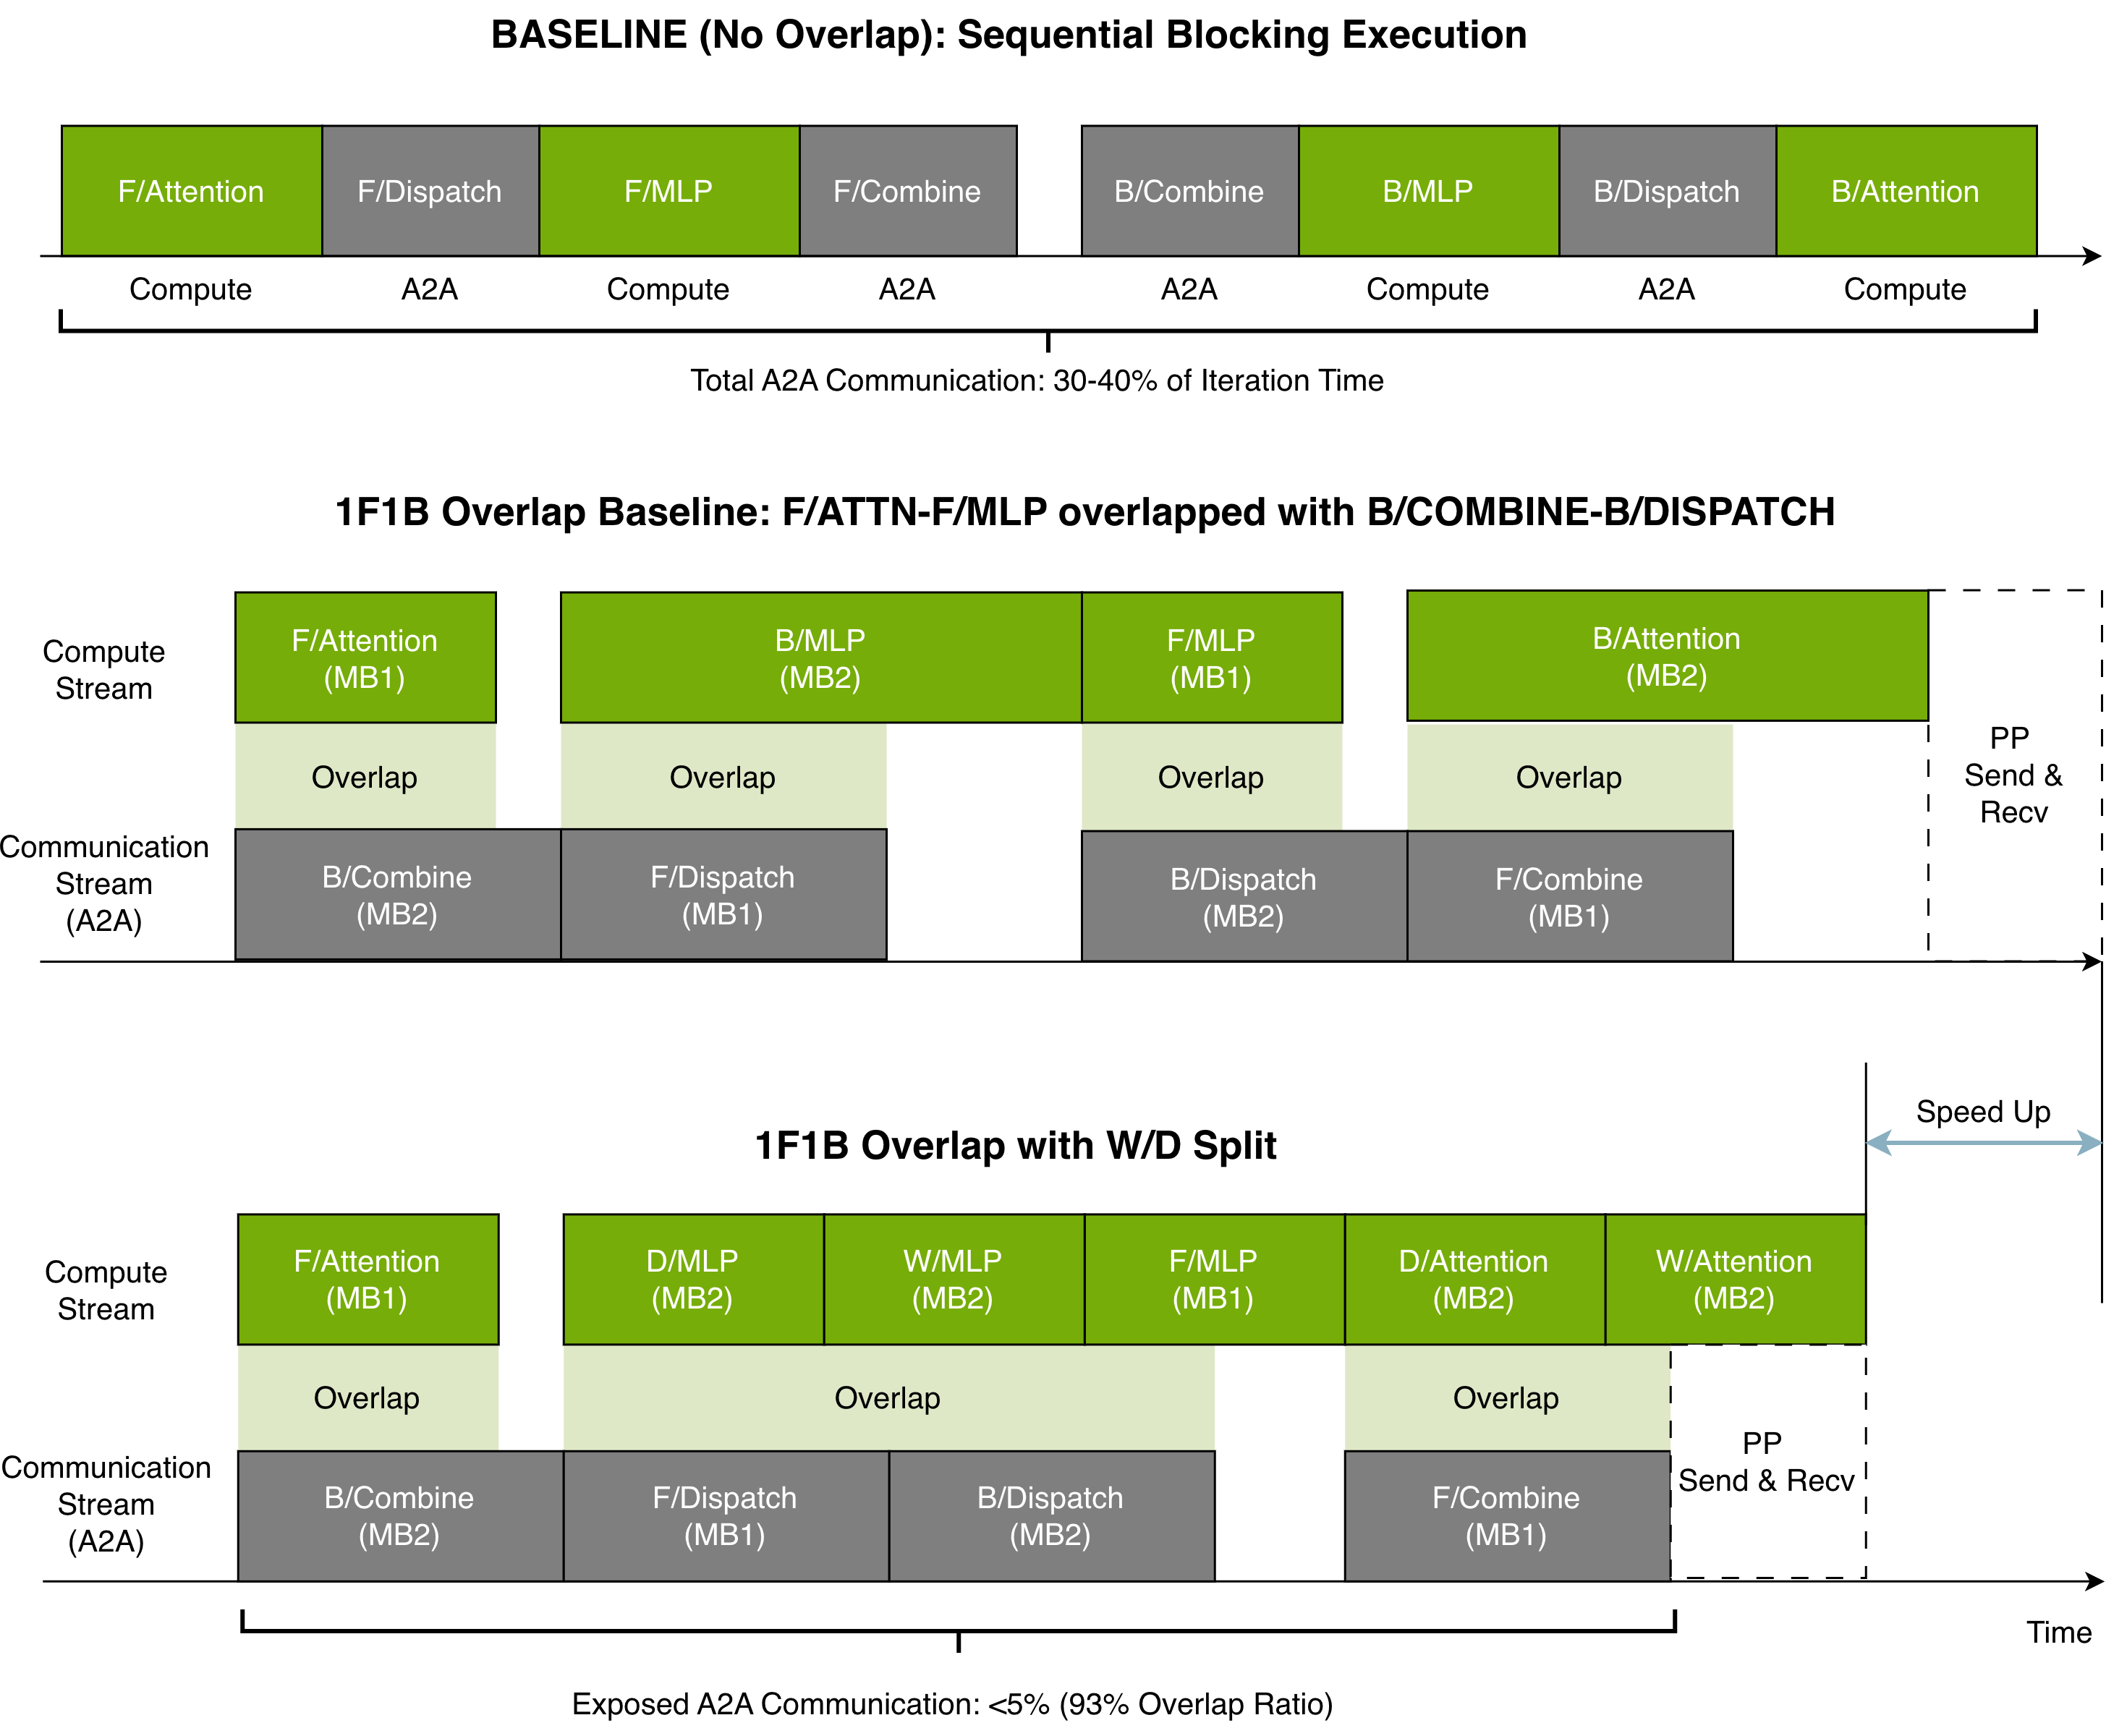
\includegraphics[width=0.9\textwidth]{figures/EP_Overlap_Summary.png}
    \caption{EP 全面通信重叠策略：基线与 W/D 分离的 1F1B。}
    \label{fig:ep-all-to-all-overlap}
\end{figure}

% \begin{figure}[ht]
%     \centering
%     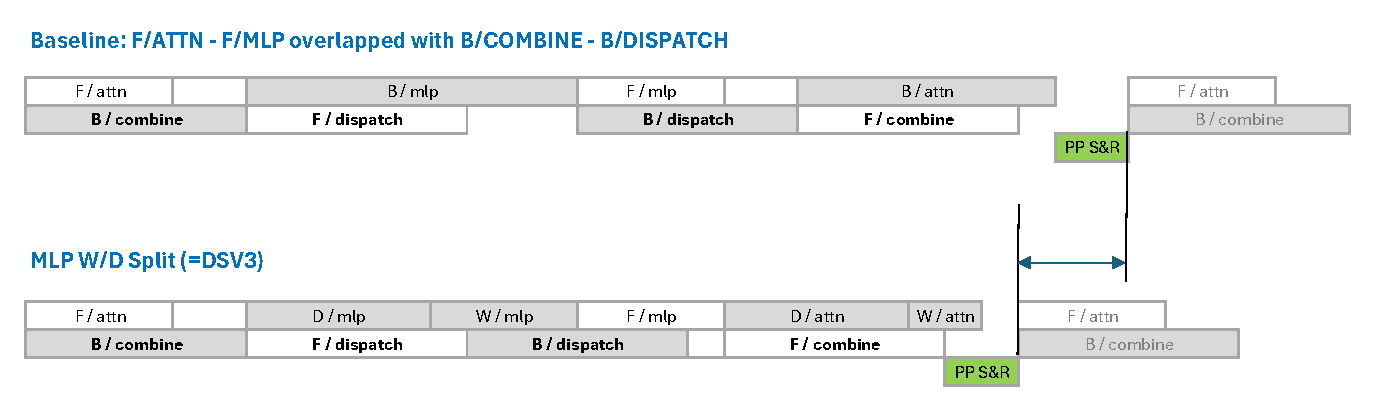
\includegraphics[width=0.8\linewidth]{figures/1f1b_split_wgrad.pdf}
%     \caption{Compute/Comm Stream Schedules}
%     \label{fig:compute_comm_streams}
% \end{figure}

为了将重叠扩展到大型模型，可以将合并的 FWD-BWD 与 \textit{交错管道并行性} （Interleaved PP），它将模型划分为虚拟管道阶段（VPP）并扩展跨管道等级的重叠机会。 \Figref{fig:interleaved_pp} 显示了具有三个阶段的交错 1F1B 时间表：预热、1F1B 和刷新。 1F1B阶段中的相邻FWD-BWD对可以应用上面的EP重叠模式。然而，当相邻对属于同一微批次时，它们仍然可能具有数据依赖性。为了避免这种情况，我们运行 \textit{一个额外的微批次} 在进入 1F1B 之前的预热结束时，确保相邻的 FWD/BWD 对无依赖性，并实现虚拟阶段之间完全的全部重叠。

合并的 FWD-BWD (1F1B) 和 DualPipeV（改进的 DualPipe 变体）之间的延迟比较显示：
\begin{itemize}
    \item \textit{1F1B 更快} 具有较大的 VPP 大小（更多虚拟阶段可实现更多重叠机会）。
    \item 在大 PP 大小和微批量计数下，延迟差距会缩小（两种策略都达到接近最佳的重叠）。
    \item 对于混合模型（例如，具有混合密集/MoE 层的 DeepSeek-V3），跨 PP 阶段的工作负载平衡至关重要。Megatron Core \textit{灵活的非对称VPP} 支持自定义每阶段层放置以最大化重叠。
\end{itemize}

\begin{figure}[ht]
    \centering
    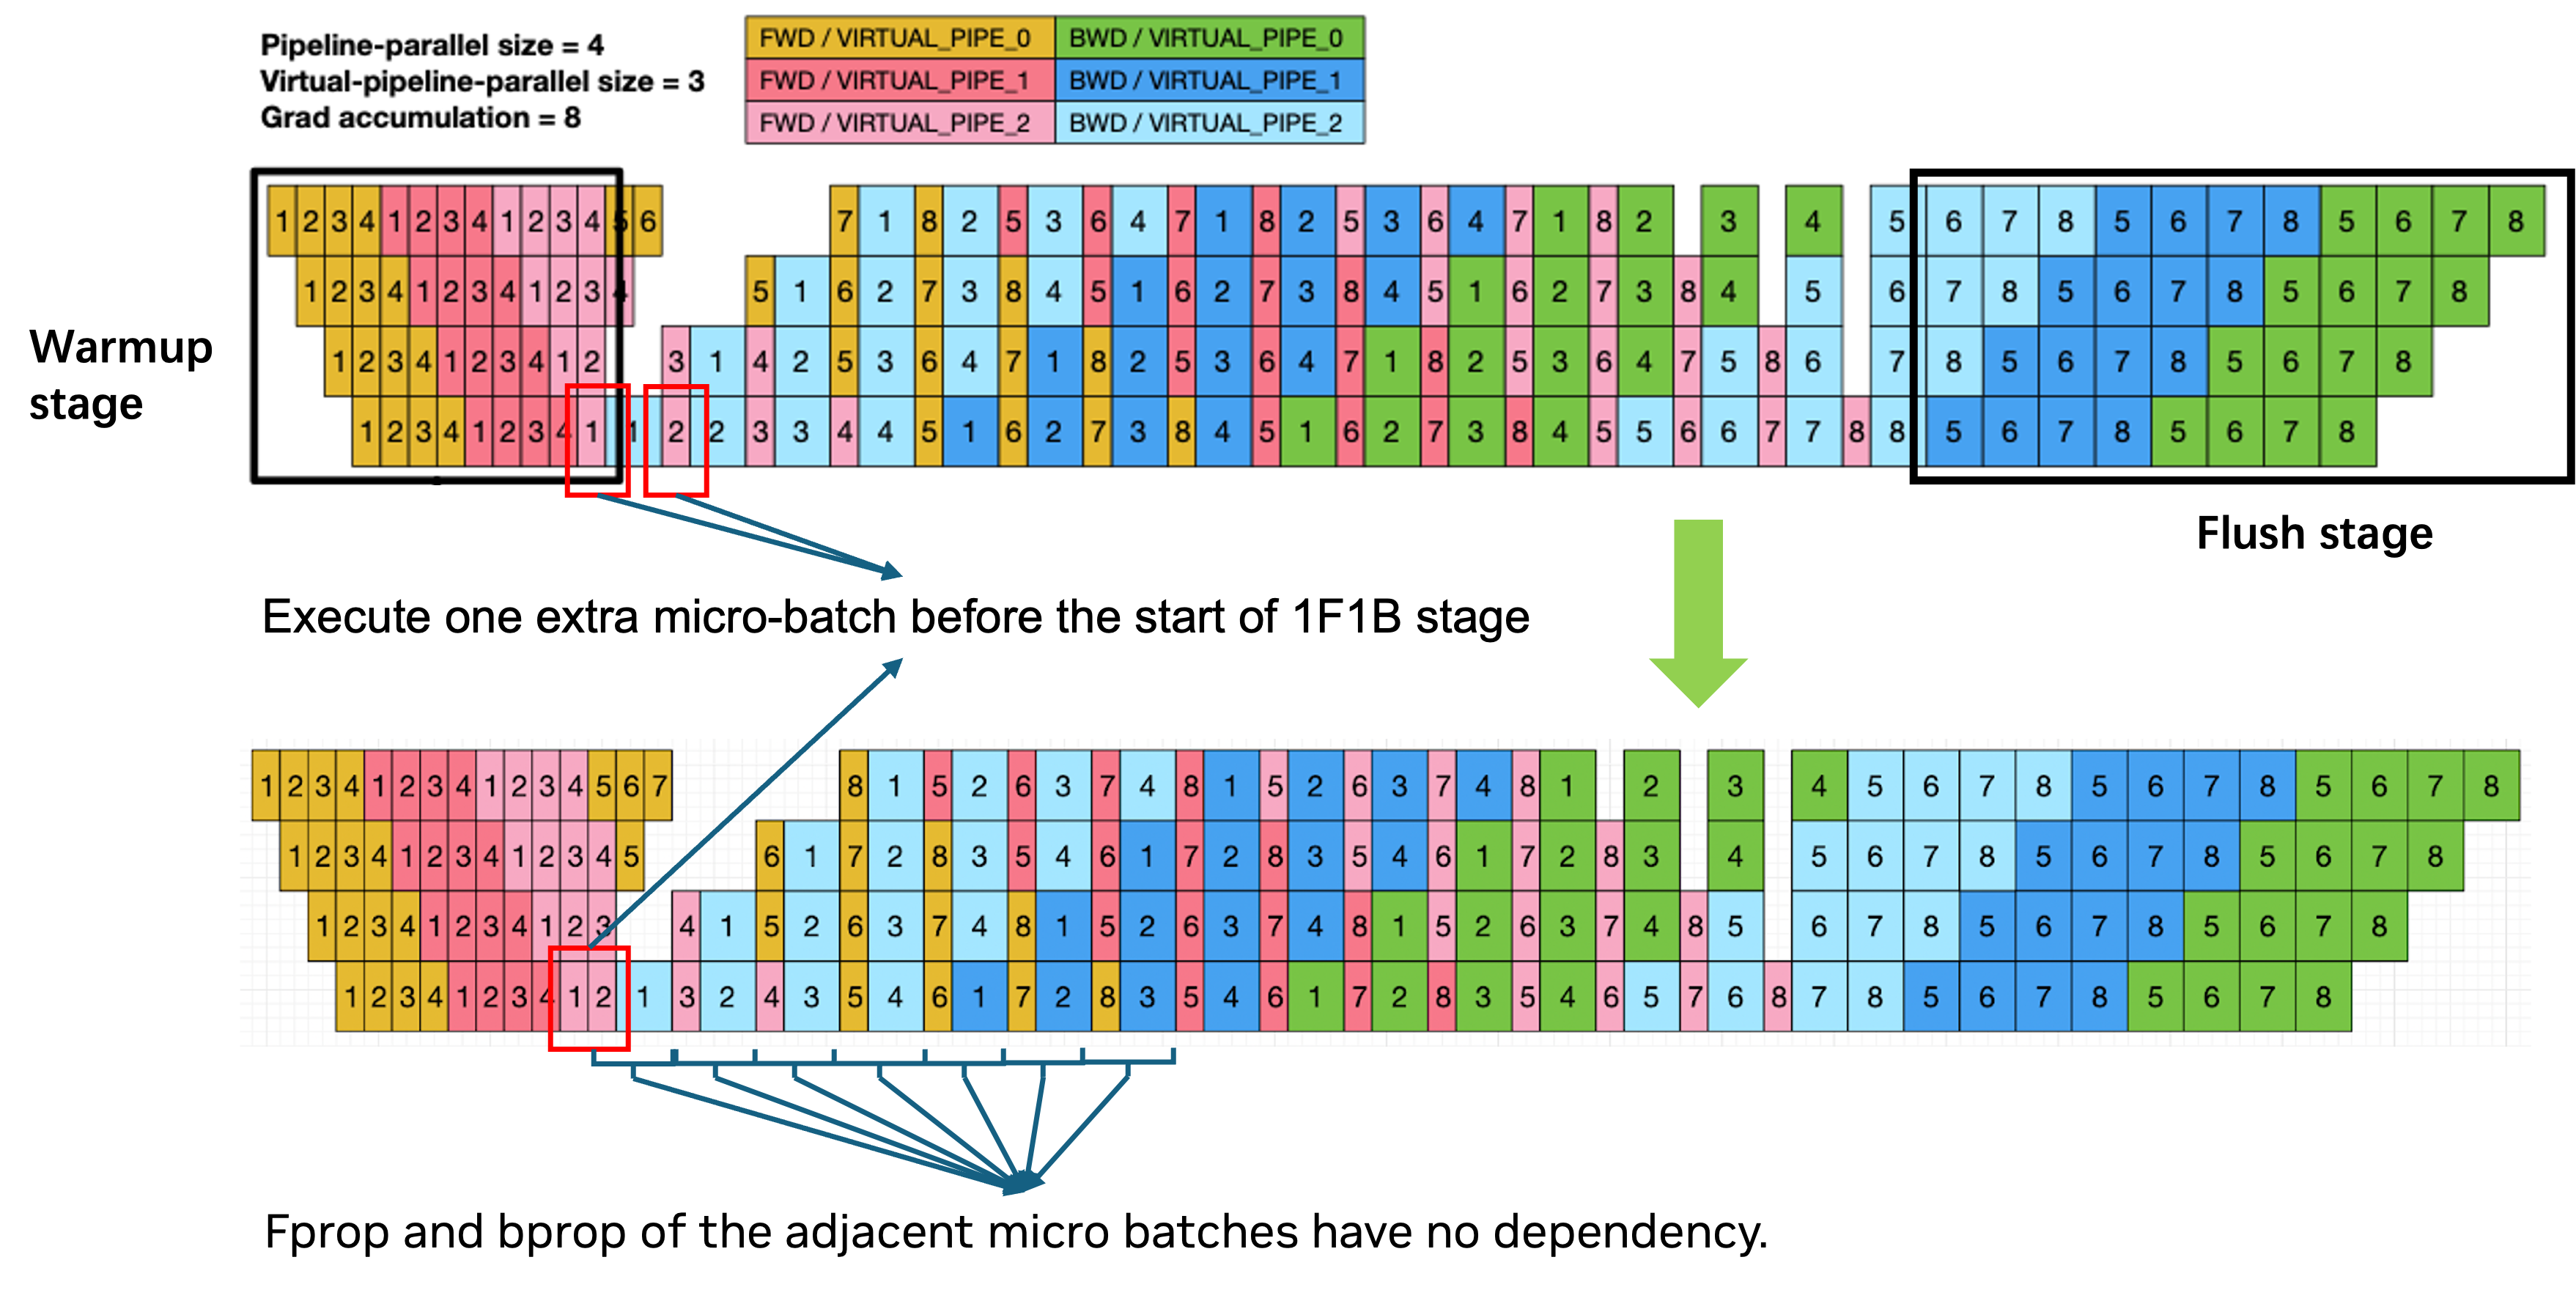
\includegraphics[width=0.9\linewidth]{figures/interleaved_pp.png}
    \caption{交错的 PP 时间线，全部重叠。}
    \label{fig:interleaved_pp}
\end{figure}

有几个因素限制了全部重叠可实现的加速：
\begin{itemize}
    \item \textbf{批次重叠比例}：更多的微批次会增加重叠批次的比例。
    \item \textbf{全部与全部的比例}：当 all-to-all 占主导地位时，EP 重叠增益更大，特别是对于计算通信比较低的跨节点 EP 和细粒度 MoE 模型。
    \item \textbf{SM 剥离管理费用}：为all-to-all保留SM会降低GEMM效率。在我们的 DeepSeek-V3 基准测试中，DeepEP 每个 GPU 使用 20 个 SM，并引入了大约 20 个 SM\% GEMM-效率开销。
\end{itemize}

在 DeepSeek-V3 等细粒度 MoE 模型上，将所有重叠与优化调度程序相结合（第 3 节~\ref{sec:deepep}）获得93分\% 专家通信延迟的重叠率，将专家通信份额从30--40减少\% 迭代时间低于 5\%.


% \subsubsection{FP8 EP Communications: Reducing Communication Volume}\label{sec:fp8-comm}

% The optimizations above hide all-to-all latency behind computation. An orthogonal approach is to reduce the all-to-all \textit{volume} itself. By performing dispatch communication in FP8 instead of BF16, we halve the data transferred per all-to-all operation.

% However, FP8 dispatch requires careful handling depending on the FP8 recipe:
% \begin{itemize}
%     \item \textbf{Blockwise/Subchannel FP8}: Tokens must be quantized before dispatch. In backward pass, we dequantize to reconstruct high-precision input, then re-quantize because forward and backward use different quantization dimensions. Transposition may be required for Hopper Tensor Core layouts.
%     \item \textbf{MXFP8}: Similar to blockwise, though transposition is unnecessary as Blackwell Tensor Cores accept any layout, backward computation requires the input tokens to be quantized along a different dimension. As a result, dequantization and re-quantization are still needed.
% \end{itemize}

% Note that \textit{combine} communication typically remains in higher precision to avoid gradient accumulation errors. The dispatch-only FP8 strategy provides 50\% all-to-all volume reduction with minimal accuracy impact. See Section~\ref{sec:fp8-dispatch-comm} for more details.

\subsubsection{概括}
通信墙优化协同工作：DeepEP/HybridEP 最大化带宽利用率； FWD-BWD 重叠隐藏了计算背后的延迟； Interleaved PP 扩展了跨管道阶段的重叠机会；灵活的 VPP 可实现最佳的负载平衡。综合起来，它们将所有人对训练时间的贡献减少到 10 以下\%。

由于通信延迟隐藏在计算背后，因此 GPU 利用率可能很高。然而，分析揭示了计算效率墙，它有两个不同的方面： \textit{内核效率} （细粒度专家生成未充分利用 GPU 资源的小型 GEMM）以及 \textit{主机开销} （许多小操作会在内核执行之间造成间隙，GPU 会在其中等待主机的工作）。

\subsection{打破计算效率的壁垒}\label{sec:compute-wall}

计算效率是最后的限制：即使有足够的内存和隐藏的通信，如果内核效率低下或主机无法足够快地分派工作，GPU 资源也可能仍未得到充分利用。随着模型和专家数量的增长，计算效率低下的情况变得更加严重，因此优化对于实现峰值硬件利用率至关重要。

\subsubsection{计算剖析：效率低下的根源}

MoE 训练中计算效率低下的原因有两个：

\textbf{内核效率。} 细粒度的 MoE 架构产生的工作负载未充分利用 GPU 资源。 DeepSeek-V3 的 256 个小专家生成 M 尺寸为 $\sim$每个专家 128 个令牌，远低于 Tensor Core 峰值利用率所需的数千个令牌。除了专家计算之外，MoE 还引入了由许多小内核组成的复杂路由和调度操作，这些小内核单独无法使 GPU 计算能力饱和。

\textbf{主机开销。} 许多小操作会产生内核启动开销，并且 CPU 无法足够快地调度工作以保持 GPU 饱和。三个因素使情况变得更糟：
\begin{itemize}
    \item \textbf{细粒度专家}：许多单独的 GEMM，而不是少数大型 GEMM，每个 GEMM 都需要单独的内核启动。
    \item \textbf{降低精度训练}：额外的量化内核会增加启动开销。
    \item \textbf{无丢包路由}：动态令牌计数需要主机设备同步来确定张量形状，从而将 CPU 置于关键路径上。
\end{itemize}

结果是 \textit{主机界限}：GPU 内核以微秒的主机端延迟分隔开来，在分析跟踪中可以看到计算资源闲置的间隙。

内核形状由模型架构决定，如果不修改模型就无法更改。因此，优化必须针对如何组织和调度计算。五种策略共同解决计算效率低下的问题：

\begin{enumerate}
    \item \textbf{熔断器相关操作。} 内核融合将路由、排列和辅助损失计算整合到更少、更大的内核中。
    \item \textbf{低精度加速。} FP8/FP4 中的降低精度训练使用更快的 Tensor Core 运算，从而提高了相同内核形状的吞吐量。
    \item \textbf{消除每次迭代的 CPU 逻辑。} CUDA 图形捕获内核序列并以最少的主机参与重放它们。
    \item \textbf{删除主机设备同步。} 免同步执行使 GPU 内核无需等待来自主机的形状信息即可继续执行。
    \item \textbf{平衡专家负载。} ECHO 动态地将热门专家克隆到未充分利用的等级，从而减少导致某些等级在其他等级计算时等待的负载不平衡。
\end{enumerate}

以下小节介绍了按这些策略组织的技术：批处理和融合以提高内核效率（第~\ref{sec:kernel-fusion}）、低精度加速度（小节~\ref{sec:fp8-training}），用于消除主机开销的 CUDA 图（部分~\ref{sec:cuda-graphs}），无滴 MoE 的无同步执行（部分~\ref{sec:sync-free-moe}），并通过 ECHO 进行负载平衡（部分~\ref{sec:echo}).

\subsubsection{分组GEMM与内核融合：提高内核效率}\label{sec:kernel-fusion}

提高内核效率最直接的方法是将小操作合并为大操作。分组 GEMM 批量专家计算以提高硬件利用率 \cite{megablocks}，而内核融合将路由和排列操作合并到更少的内核中 \cite{chen2018tvm}。 Megatron-Core 在三个级别实现这些优化：专家计算（分组 GEMM）、令牌路由（排列融合）和路由器逻辑（路由器和 Aux-Loss 融合）。

\paragraph{分组GEMM}\label{sec:grouped-gemm}

专家的计算本质上是一系列独立的GEMM。分组 GEMM 通过重叠内核的波尾效应，比单独的顺序 GEMM 提高了性能。

Megatron-Core 提供了两种分组 GEMM 实现：

\begin{itemize}
\item[i.] cuBLASLt GEMM 的多流启动。
通过将各个 cuBLASLt GEMM 启动到多个 CUDA 流中，它们可以彼此重叠。该方法支持各种精度和缩放模式，包括 BF16、每张量 FP8、块式 FP8、MXFP8 和 NVFP4，其性能与高度优化的分组 GEMM 实现相当。

\item[ii.]\label{gmm:2} CUTLASS 分组 GEMM。
通过将各个 GEMM 融合到单个内核中，当 GEMM 数量很大时，CUTLASS Grouped GEMM 可以获得更好的性能。然而，不同的精度、缩放模式和硬件平台需要单独的开发工作，并且需要针对不同的问题规模进行额外的调整。 TE 当前的实现仅支持 Hopper 平台上的 BF16。
\end{itemize}


另外两个实现正在开发中：

\begin{itemize}
\item[iii.] cuBLASLt 分组 GEMM 通过 \texttt{CUBLASLT\_BATCH\_MODE\_GROUPED}。
cuBLASLt 分组 GEMM 假设设备上的形状信息并在单个内核中进行计算，这消除了将 CUDA 图形应用于专家部分的障碍。它涵盖了具有内置启发式的所有精度和缩放模式，并且旨在在支持的情况下取代 (i) 和 (ii)。

\item[iv.] CuteDSL 具有融合功能的分组 GEMM。
分组 GEMM 与激活函数、量化（用于下一层）和通过cuteDSL 缩放因子混合融合。这些内核针对 MXFP8 和 NVFP4 进行了优化~\cite{abecassis2025nvfp4} 在 Blackwell 平台上，针对 \texttt{fprop} FC1的GEMM和 \texttt{dgrad} FC2的GEMM。通过将专家计算、激活和量化整合到单个内核中，该方法显着减少了内核数量，并且与 CUDA 图形兼容。
\end{itemize}

\subsubsection{排列融合}

目前，分组 GEMM 要求分配给同一专家的令牌连续存储（即排列令牌）。如果启用了所有人对所有人的集体通信，则需要进一步排列以确保分配给每个等级的令牌被分组在一起。使用本机 PyTorch 实现高效排列具有挑战性，因为它往往会启动许多小内核并产生额外的 CPU 开销。

训练工作负载中的置换融合管道（\figref{fig:permute_fusion}）由三个阶段组成：

\begin{figure}[ht]
    \centering
    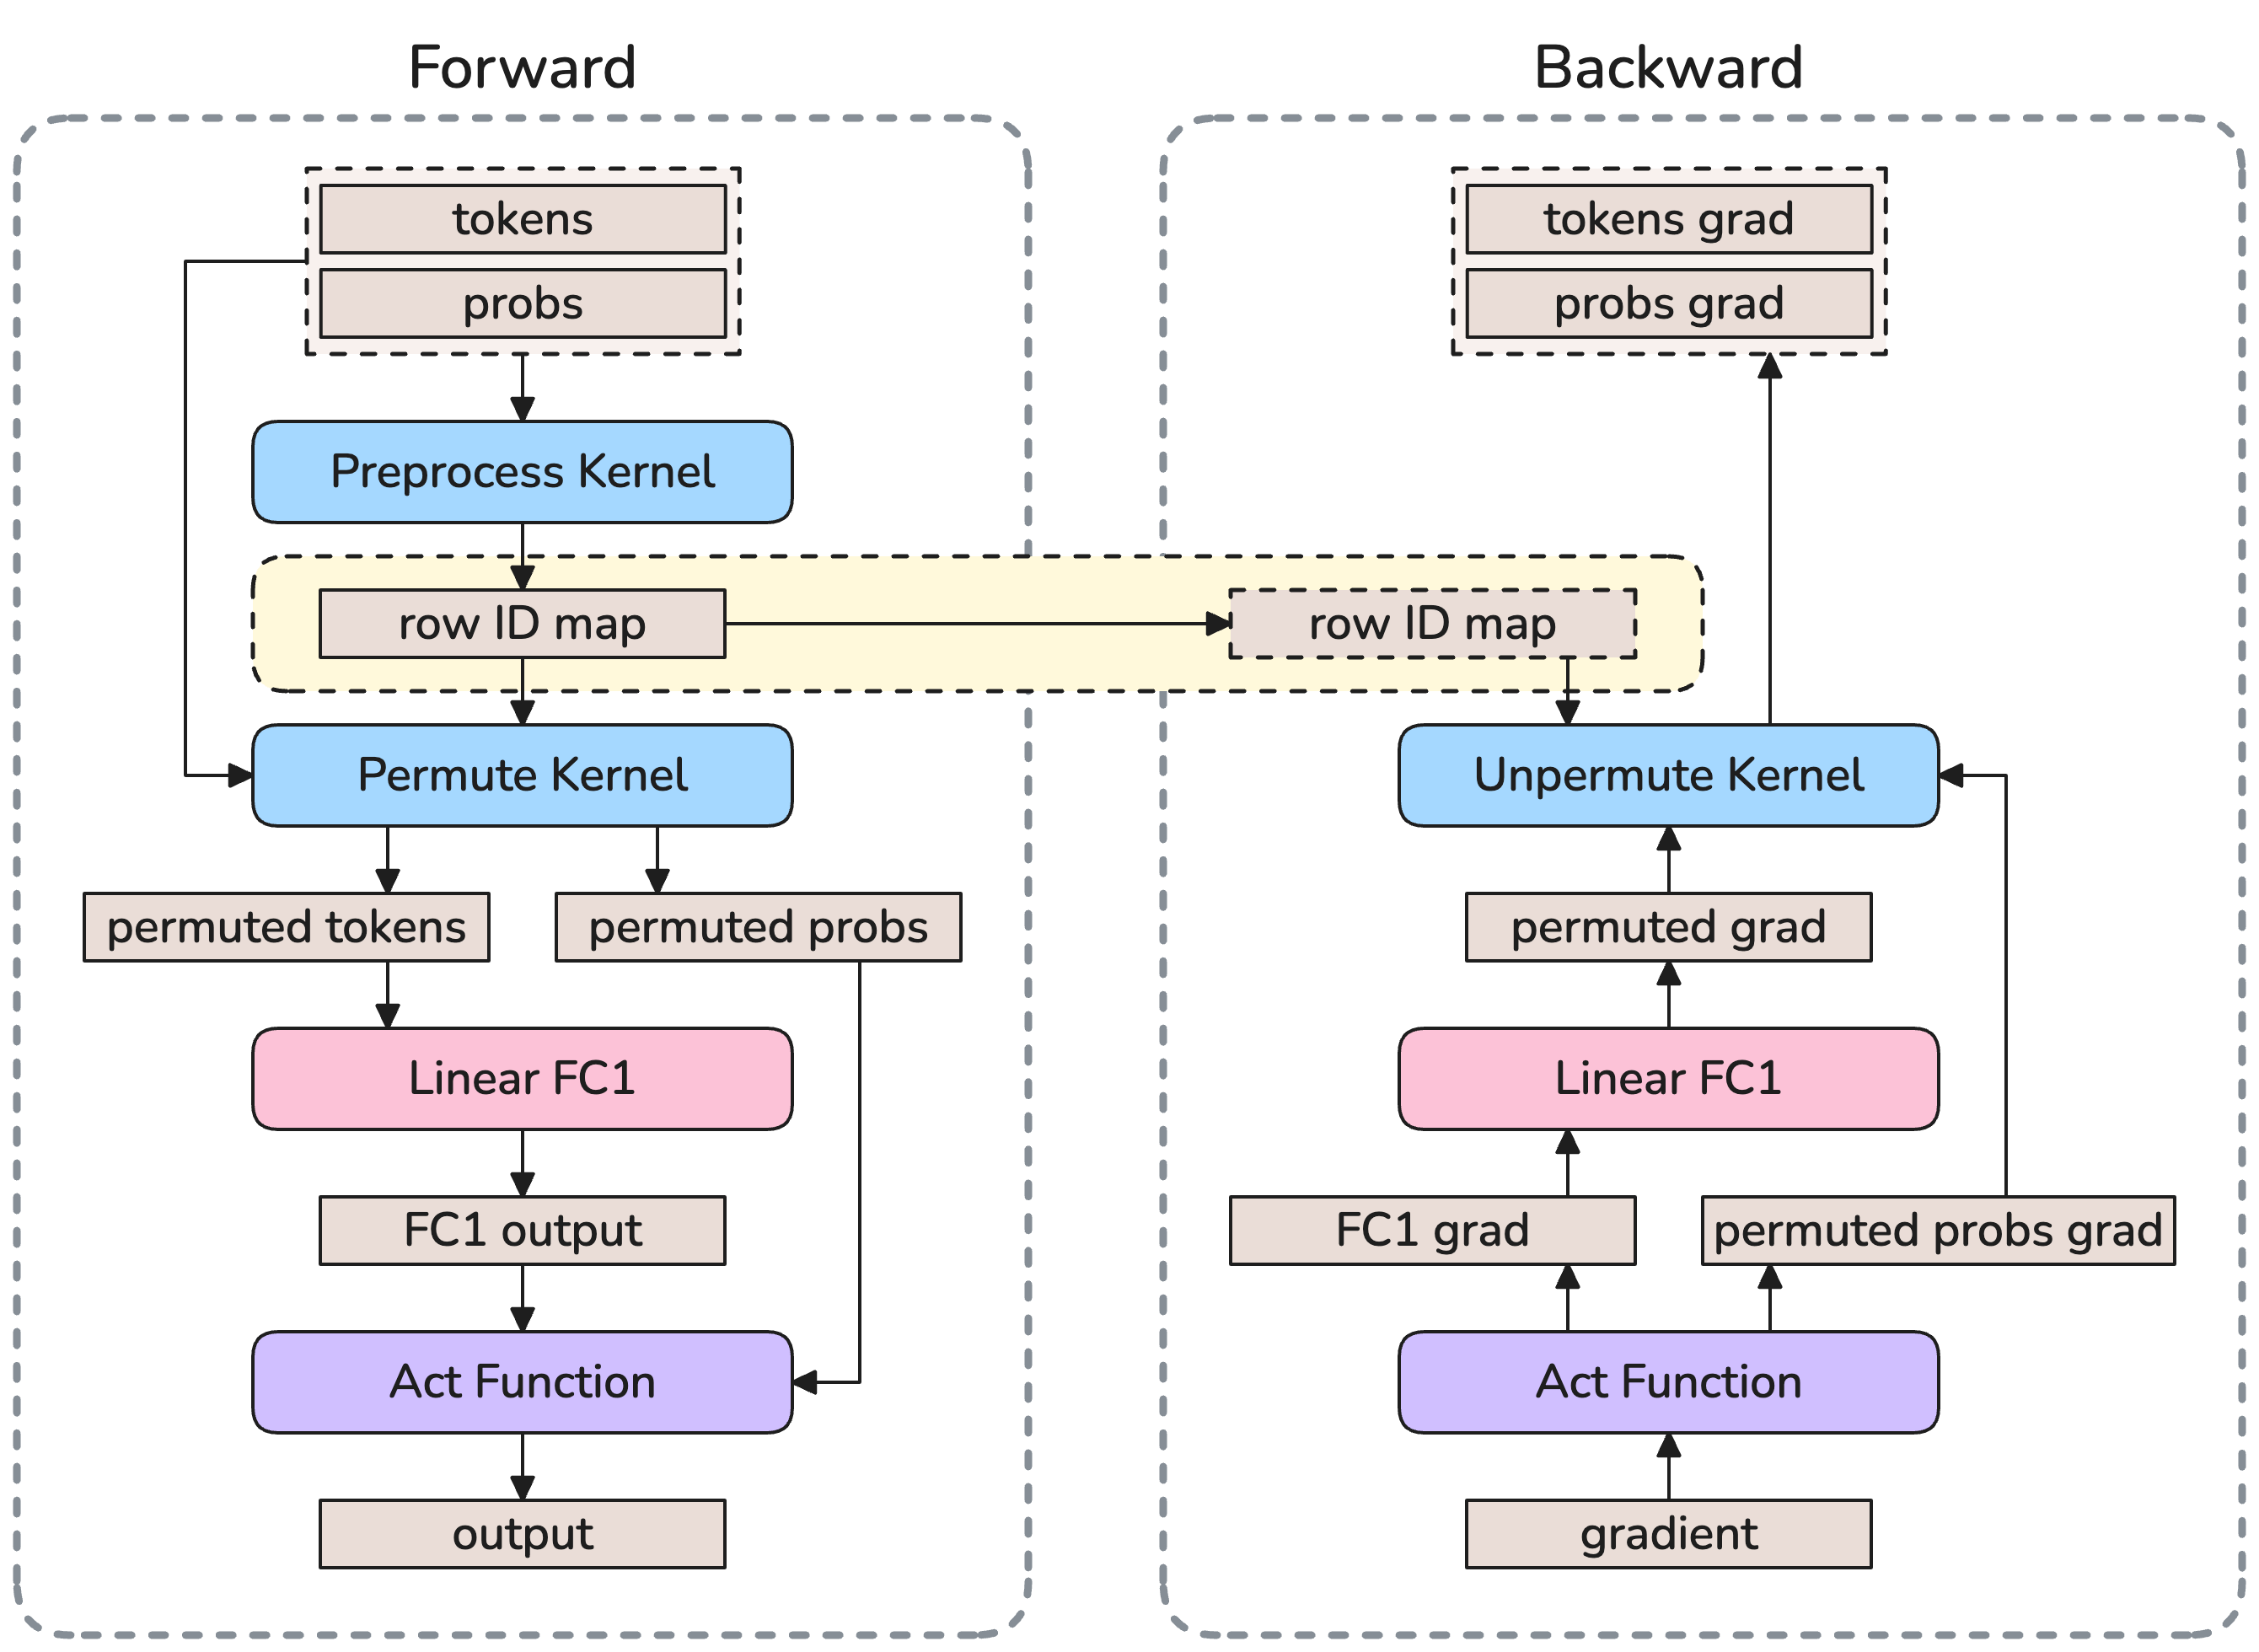
\includegraphics[width=0.6\linewidth]{figures/permute_fusion.png}
    \caption{训练过程中置换融合的管道。}
    \label{fig:permute_fusion}
\end{figure}

\begin{itemize}
    \item 预处理：排列本质上是一个数据传输过程，需要将令牌连续存储在每个专家对应的缓冲区中。预处理步骤的目的是生成偏移图（Row ID map in \figref{fig:permute_fusion})，它表示每个标记在输入和输出缓冲区中的偏移量。这确保了可以有效地执行置换和取消置换操作。在前向传递过程中，预处理内核在排列之前仅调用一次，而其他组件则重用结果。
    \item 置换：置换内核的功能很简单：它根据偏移映射将令牌从输入缓冲区移动到输出缓冲区，然后将它们传递给后续的专家 MLP。在内存高效排列中，也需要对概率进行排列，结果直接进入EA的激活部分。
    \item 取消排列：取消排列步骤是排列操作的逆过程。由于在排列期间令牌将被多次复制并发送到不同的目的地，因此必须在组合阶段将这些令牌求和在一起。在内存高效的排列中，组合步骤只是将它们相加；否则，概率将用作权重。所有累加均以 FP32 精度执行。
\end{itemize}

\subsubsection{路由器和 Aux-Loss 融合}

路由器及辅助损耗 \cite{fedus2022switchtransformersscalingtrillion,zoph2022stmoe,hwang2023tutel,rajbhandari2022deepspeedmoe} 计算是生成许多小内核并引入大量 CPU 开销的其他领域。随着设备计算能力的增长，融合变得越来越重要。

挑战在于路由器包含难以融合的组件，例如GEMM和通信。我们将剩余的操作分解为三个部分，每个部分融合成一个内核（\figref{fig:router_fusion}).
\begin{figure}[ht]
    \centering
    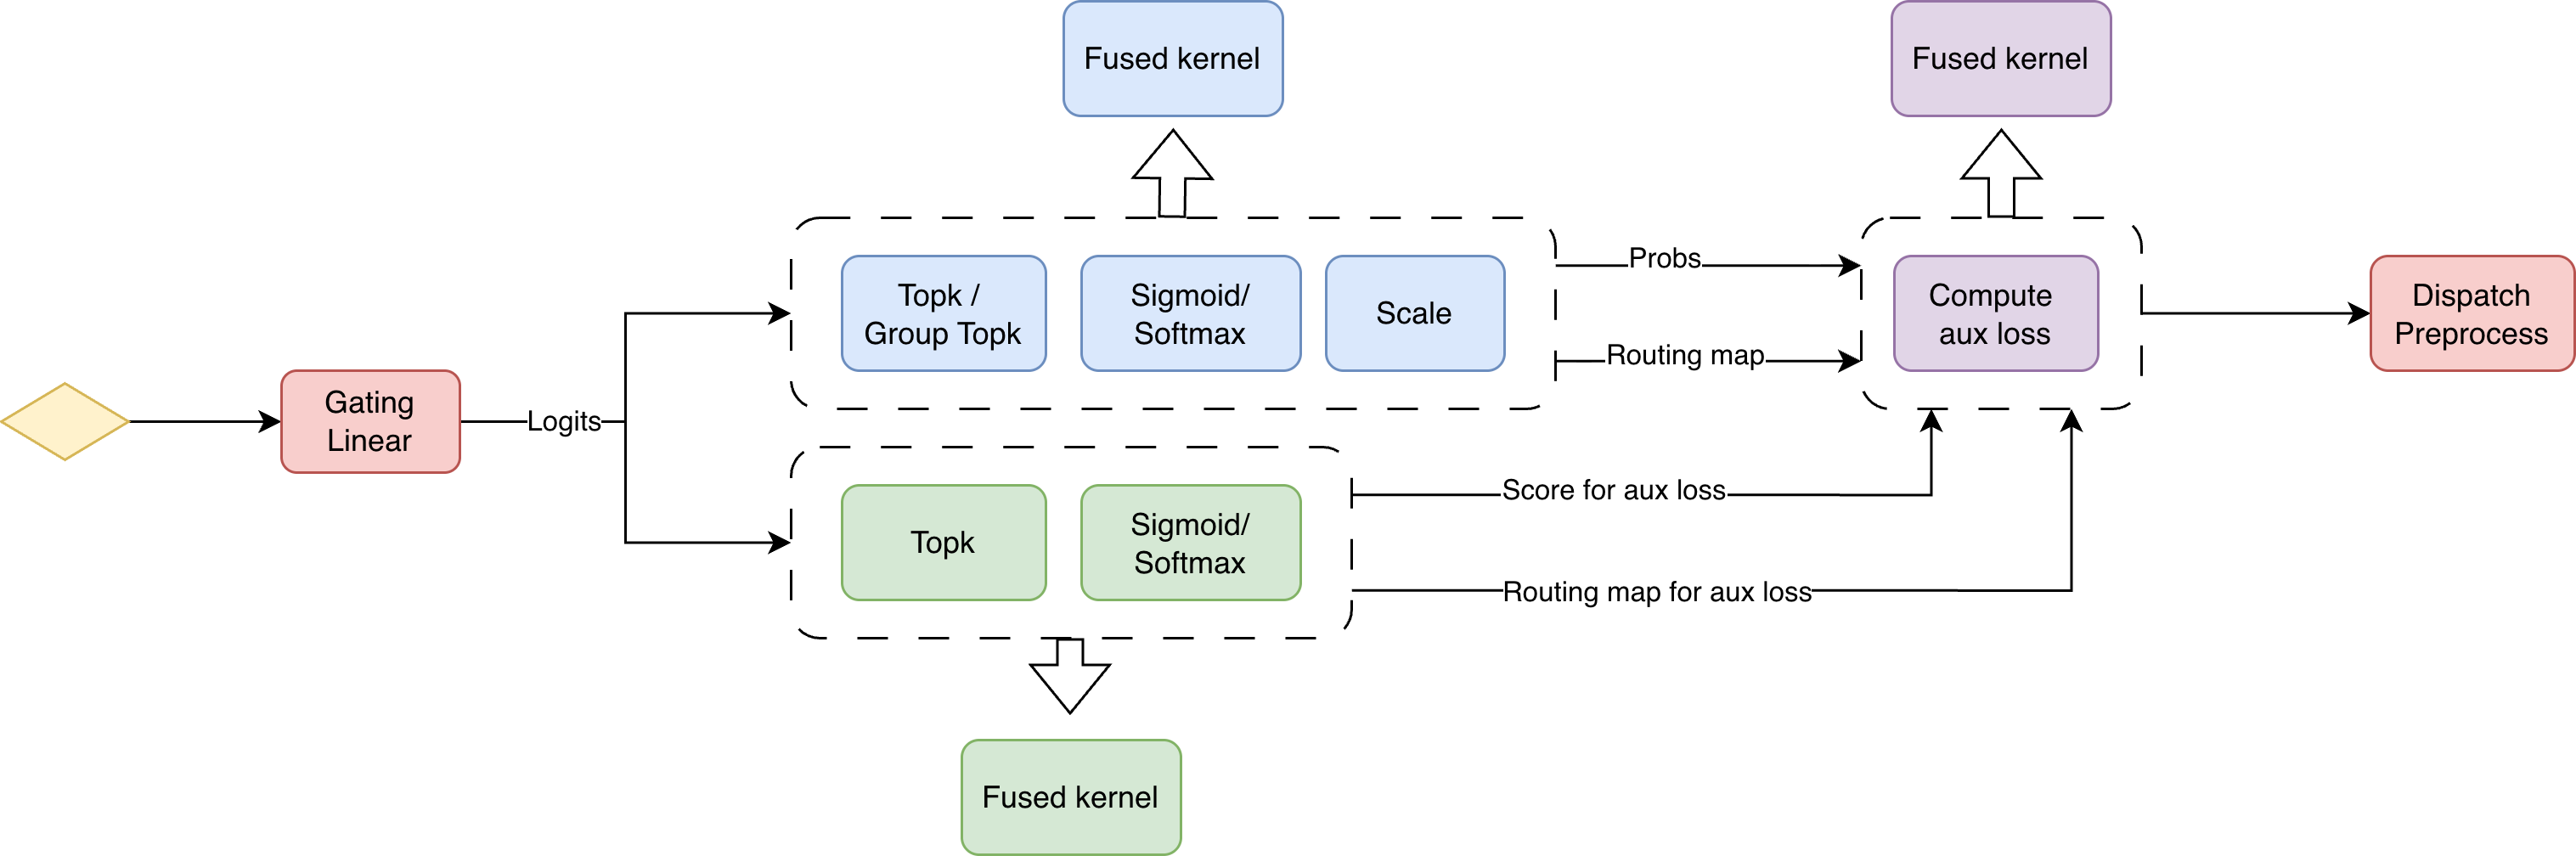
\includegraphics[width=1\linewidth]{figures/router_fusion.drawio.png}
    \caption{路由器融合的工作流程。}
    \label{fig:router_fusion}
\end{figure}
\begin{itemize}
    \item 分数计算，包括top-$k$ softmax/sigmoid：这是最复杂的函数，针对不同的模型有不同的分支。它包括不同的顶部$k$ 算法（朴素的顶$k$, 组顶-$k$ \cite{deepseekai2024deepseekv2strongeconomicalefficient,deepseekai2025deepseekv3technicalreport}）、评分函数（sigmoid、softmax）、它们的组合以及可能的缩放操作。
    \item 辅助损失的分数计算：这是第一部分的子集。在得分函数和朴素的顶部之后$k$ 计算时，生成辅助损失计算的输入。
    \item MoE辅助损失的计算：在步骤2的基础上，辅助损失计算被融合到单个内核中。

\end{itemize}
启用路由器融合后，路由器模块内的工作流程如图所示 \figref{fig:router_fusion}。未来的工作可能会将通信纳入融合范围。

\subsubsection{降低精度训练：低精度加速}\label{sec:fp8-training}

具有小型专家 GEMM 的细粒度 MoE 工作负载通常会受到内存带宽的限制，从而限制了 Tensor Core 的利用率。降低精度训练通过减少数据移动并在 Hopper 和 Blackwell GPU 上使用更快的 FP8/FP4 张量核心运算来解决这个问题。

从计算效率的角度来看，降低精度的训练提供了一个关键的好处： \textbf{FP8/FP4 GEMM} 通过在 FP8/FP4 中执行线性层计算来最大化 Tensor Core 利用率。再加上Sections中的记忆好处~\ref{sec:fp8-activation}，FP8训练大约达到 \textbf{10\% 至 25\% 端到端性能改进} 用于不同硬件平台上的大规模 MoE 训练，而 FP4 则提供了更多加速。

有关降低精度的训练方法、MoE 特定挑战和量化策略的完整介绍，请参阅第 4 节~\ref{sec:reduced-precision-training}.

\subsubsection{CUDA 图：消除主机开销}\label{sec:cuda-graphs}

内核融合减少了 \emph{数字} 内核启动次数； CUDA 图消除了 \emph{每次迭代成本} 这些发射。本小节介绍 CUDA Graph 如何解决 CPU 开销、drop-and-pad 与 dropless MoE 的不同策略，以及使 CUDA Graph 实用所需的内存优化。

在 MoE 训练中，CPU 开销往往成为主要的性能瓶颈。这种开销来自三个来源：
\begin{enumerate}
    \item \textbf{Python执行}：解释器开销、C 外部函数接口 (CFFI) 和垃圾收集会引入延迟。
    \item \textbf{框架开销}：即使是简单的操作，例如 \texttt{torch.empty} 增加主机端成本的微秒级；库层（TransformerEngine、cuBLAS、cuDNN）添加更多。
    \item \textbf{内核启动开销}：每次内核启动都会产生几微秒的 CPU 端成本。
\end{enumerate}

现代培训中的三个趋势放大了这一点：
\begin{itemize}
    \item \textbf{更快的 GPU}：随着内核执行速度的提高，重叠 CPU 工作的时间越来越少，使得 CPU 开销越来越明显。
    \item \textbf{MoE复杂性}：MoE 模型给 FFN 层（路由器、调度、分组 GEMM 和组合操作）增加了相当大的复杂性，产生了许多超出 GEMM 本身的小内核，从而产生了大量的 CPU 开销。
    \item \textbf{降低精度训练}：额外的量化内核，特别是在细粒度的 MoE 中，其中操作计数与专家的数量成比例。
\end{itemize}

\begin{figure}[ht]
    \centering
    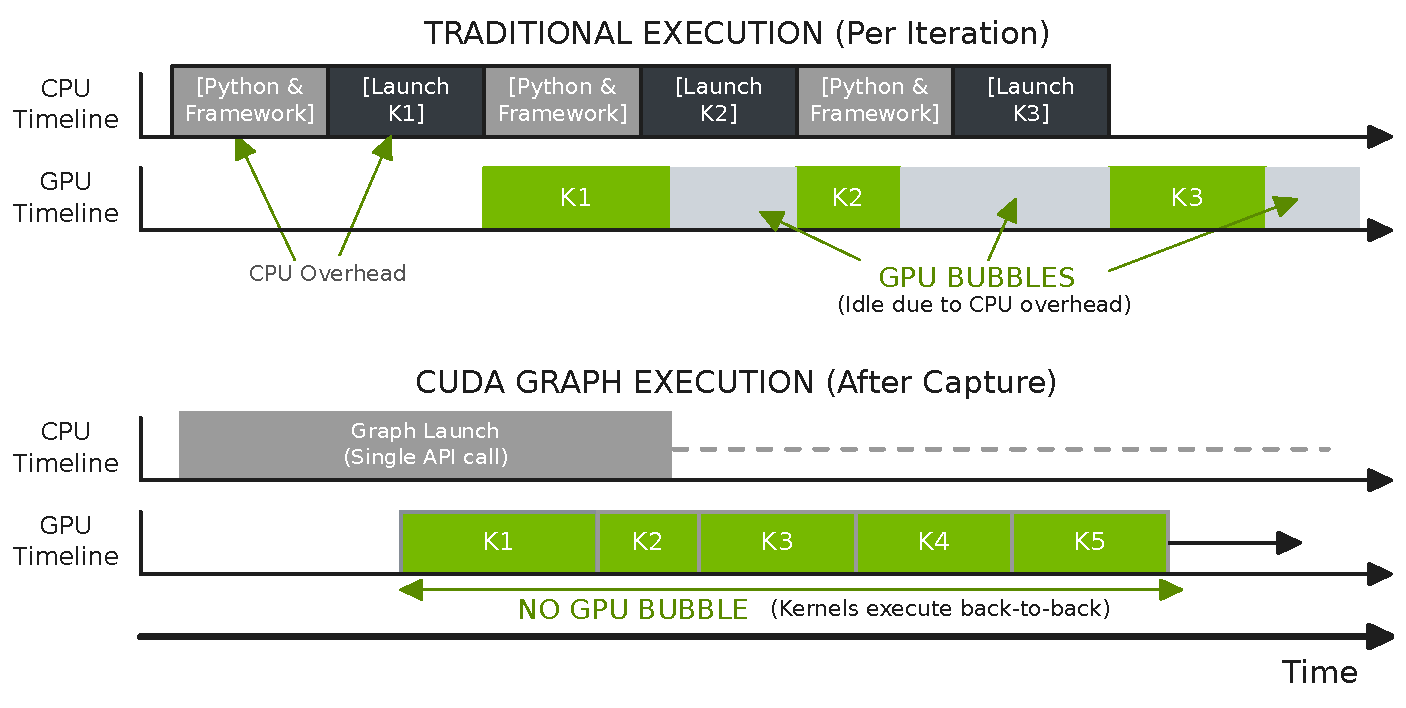
\includegraphics[width=0.8\textwidth]{figures/cuda_graph_comparison.pdf}
    \caption{传统执行（顶部）与 CUDA 图形执行（底部）。}
    \label{fig:cuda-graph-execution-comparison}
\end{figure}

% Nsight Systems profiling of non-CUDA Graph MoE training (the upper half of \figref{fig:partial_cudagraph_nsys}) 
\Figref{fig:cuda-graph-execution-comparison} 显示了传统执行管道中巨大的 CPU 开销和由此产生的 GPU 气泡，揭示了 GPU 内核之间的巨大差距。这清楚地表明 CPU 无法足够快地启动内核来充分利用 GPU，这种现象称为 CPU 开销或主机限制。
CUDA 图通过在初始迭代期间将一系列 GPU 内核捕获到可重播图中来解决此问题 \cite{nvidia_cudagraphs,ansel2024pytorch2}。随后的迭代会发出一个 \textit{图表发布} 调用，很大程度上绕过了每个操作 Python/框架的开销和每个内核启动的开销，从而减少了 CPU 端的延迟。

然而，CUDA Graph 要求所有捕获的操作都具有 \textbf{静态的、预定的形状}。动态形状或控制流会导致图形捕获失败。这与 MoE 产生了根本性的紧张关系，每个专家的令牌数量动态变化。下一段描述了 Megatron-Core 的两种 CUDA 图形模式——完整 CUDA 图形和分层 CUDA 图形——以及它们如何解决 MoE 中的动态形状约束。

\begin{figure}[ht]
    \centering
    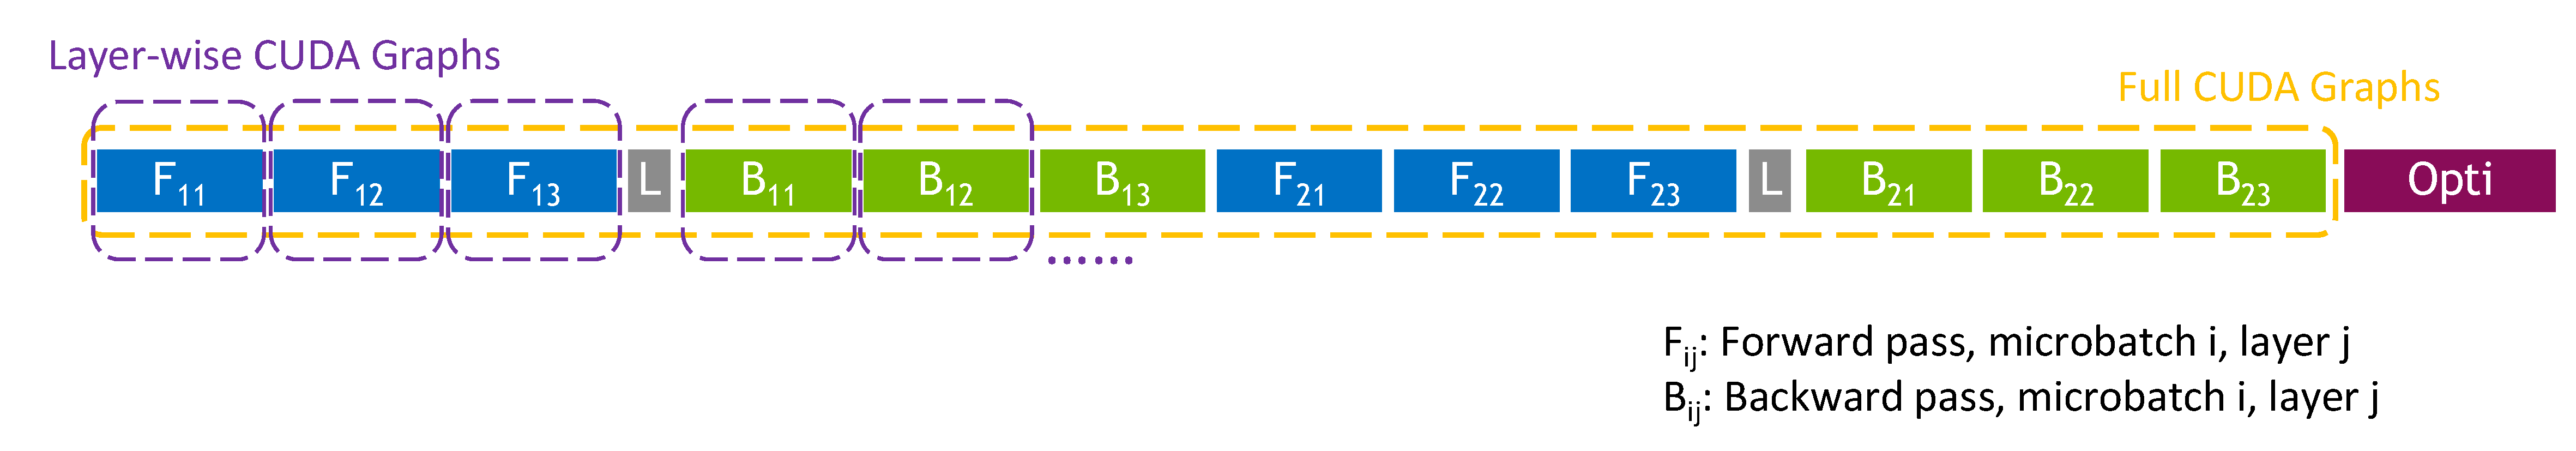
\includegraphics[width=0.95\linewidth]{figures/full_iter_layerwise.pdf}
    \caption{一次训练迭代中的完整 CUDA 图与分层 CUDA 图（三层，两个微批次）。}
    \label{fig:full_iter_layerwise}
\end{figure}

\paragraph{完整 CUDA 图与分层 CUDA 图}

如图所示 \figref{fig:full_iter_layerwise}，Megatron-Core 支持两种类型的 CUDA 图：完整 CUDA 图和分层 CUDA 图。 \textit{满的} CUDA 图，也称为全迭代 CUDA 图，将整个前向-后向传递捕获到单个 CUDA 图中。仅支持使用的密集或 MoE 模型 \textbf{带填充的令牌丢弃}，表示每个专家有固定的接收能力；超出容量的令牌将被丢弃，并填充输入以确保恒定的张量形状。在所有形状都是静态的情况下，可以将整个迭代绘制成图表，从而最大限度地减少 CPU 开销。至于 \textbf{无滴的} MoE 模型（例如 DeepSeek-V3）无法删除路由令牌，完整的 CUDA 图是不可行的，因为分配给每个专家的令牌数量根据路由决策动态变化。专家 GEMM 形状在迭代之间发生变化，违反了静态形状要求。此外， \textit{设备-主机同步} 需要检索每个专家的令牌计数以进行调度。部分~\ref{sec:sync-free-moe} 描述了我们为克服动态调度和同步问题所做的努力，以便完整的 CUDA 图也可以应用于无滴 MoE。或者，这里我们介绍一种基于分层 CUDA 图的更简单的方法，称为 \textit{部分的} CUDA 图形。

\begin{comment}
Megatron-Core supports full-iteration CUDA Graph for drop-and-pad MoE models via the \texttt{local} implementation:

\begin{lstlisting}
--moe-expert-capacity-factor 1.0 \
--moe-pad-expert-input-to-capacity \
--cuda-graph-impl local \
--cuda-graph-scope full_iteration
\end{lstlisting}
\end{comment}

% Instead of capturing the entire forward-backward pass into a single CUDA Graph, layer-wise CUDA Graphs capture each transformer layer separately. Note that both full CUDA Graphs and layer-wise CUDA Graphs are natively \textbf{not feasible for dropless MoE models} such as DeepSeek-V3, where no routed tokens can be dropped, so the number of tokens assigned to each expert varies dynamically based on routing decisions. Expert GEMM shapes change from iteration to iteration, violating the static-shape requirement. Additionally, \textit{device-host synchronization} is required to retrieve per-expert token counts for dispatching. Section~\ref{sec:sync-free-moe} describes our effort to overcome the dynamic dispatching and synchronization issues so that the full CUDA Graphs (either the full-iteration CUDA Graphs or full-layer-wise CUDA Graphs) can also be applied to dropless MoE. Alternatively, here we introduce a simpler method based on layer-wise CUDA Graph, called partial CUDA Graphs, which selectively captures only the \textbf{static components} of each MoE layer while leaving dynamic parts outside the graph, achieving significant performance gains for dropless MoE despite not capturing the entire model.

\begin{figure}[ht]
    \centering
    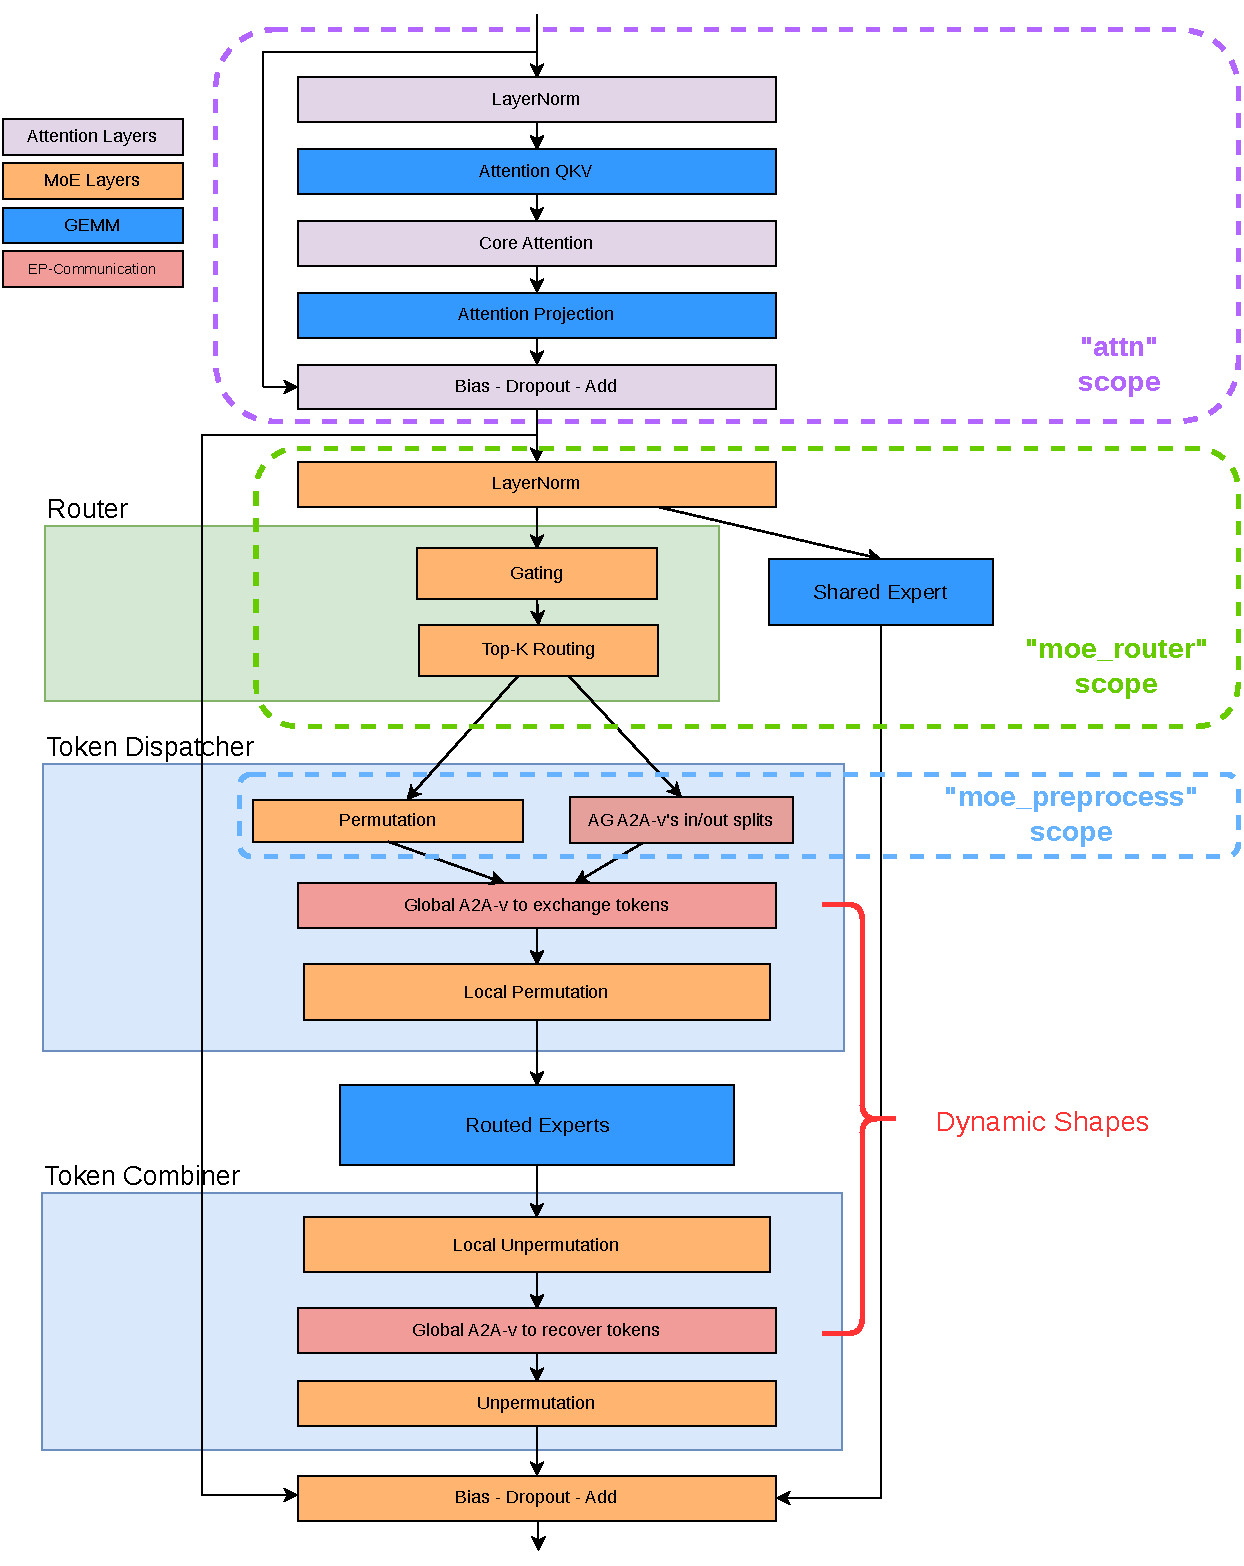
\includegraphics[width=0.6\linewidth]{figures/partial-cudagraph.pdf}
    \caption{部分 CUDA 图捕获静态组件（注意力、共享专家、路由器、预处理），同时将动态专家计算留在图之外。}
    \label{fig:partial_cudagraph}
\end{figure}

逐层 CUDA 图表分别捕获每个转换器层。与完整的 CUDA 图表一样，捕获整个Transformer层仍然会在 MoE 部分中遇到动态形状。部分 CUDA 图通过仅捕获 \textbf{静态组件} 的每一层，同时将动态部分留在图形之外，即使没有捕获完整模型，也可以为无滴 MoE 带来巨大的性能提升。在无滴 MoE 层中：

\begin{itemize}
    \item \textbf{静态组件} （可以用图表表示）：
    \begin{itemize}
        \item 注意力层（处理固定数量的标记）
        \item 路由器计算（固定输入/输出形状）
        \item 专家并行 (EP) 预处理（静态排列元数据）
        \item 共享专家（如果存在，处理具有固定形状的所有标记）
        \item 稠密 Transformer块中的 MLP 层
    \end{itemize}

    \item \textbf{动态组件} （无法绘制图表）：
    \begin{itemize}
        \item 令牌分发（从固定形状到动态形状）
        \item 专家GEMM操作（基于令牌分配的动态M维度）
        \item Token组合（从动态形状到固定形状）
    \end{itemize}
\end{itemize}

部分 CUDA 图独立捕获每层的静态部分，使路由专家计算正常执行。
如图所示 \figref{fig:partial_cudagraph}，每个Transformer层的前向路径被分成几个“范围”，用户可以选择要绘制哪些范围。随着“\textit{收件人+MoE\_路由器+萌系\_预处理}“范围启用，一个图捕获该层的调度操作之前的所有静态组件：注意力、路由器（投影、顶部）$k$ 选择和辅助损失计算）和EP预处理（令牌元数据计算和排列）。该图中还捕获了共享专家（如果存在）。这种方法允许动态专家计算以不同的形状执行，从而消除了 CPU 开销，同时保持了正确性。尽管没有捕获整个模型，但这仍取得了显着的性能提升。

\begin{figure}[ht]
    \centering
    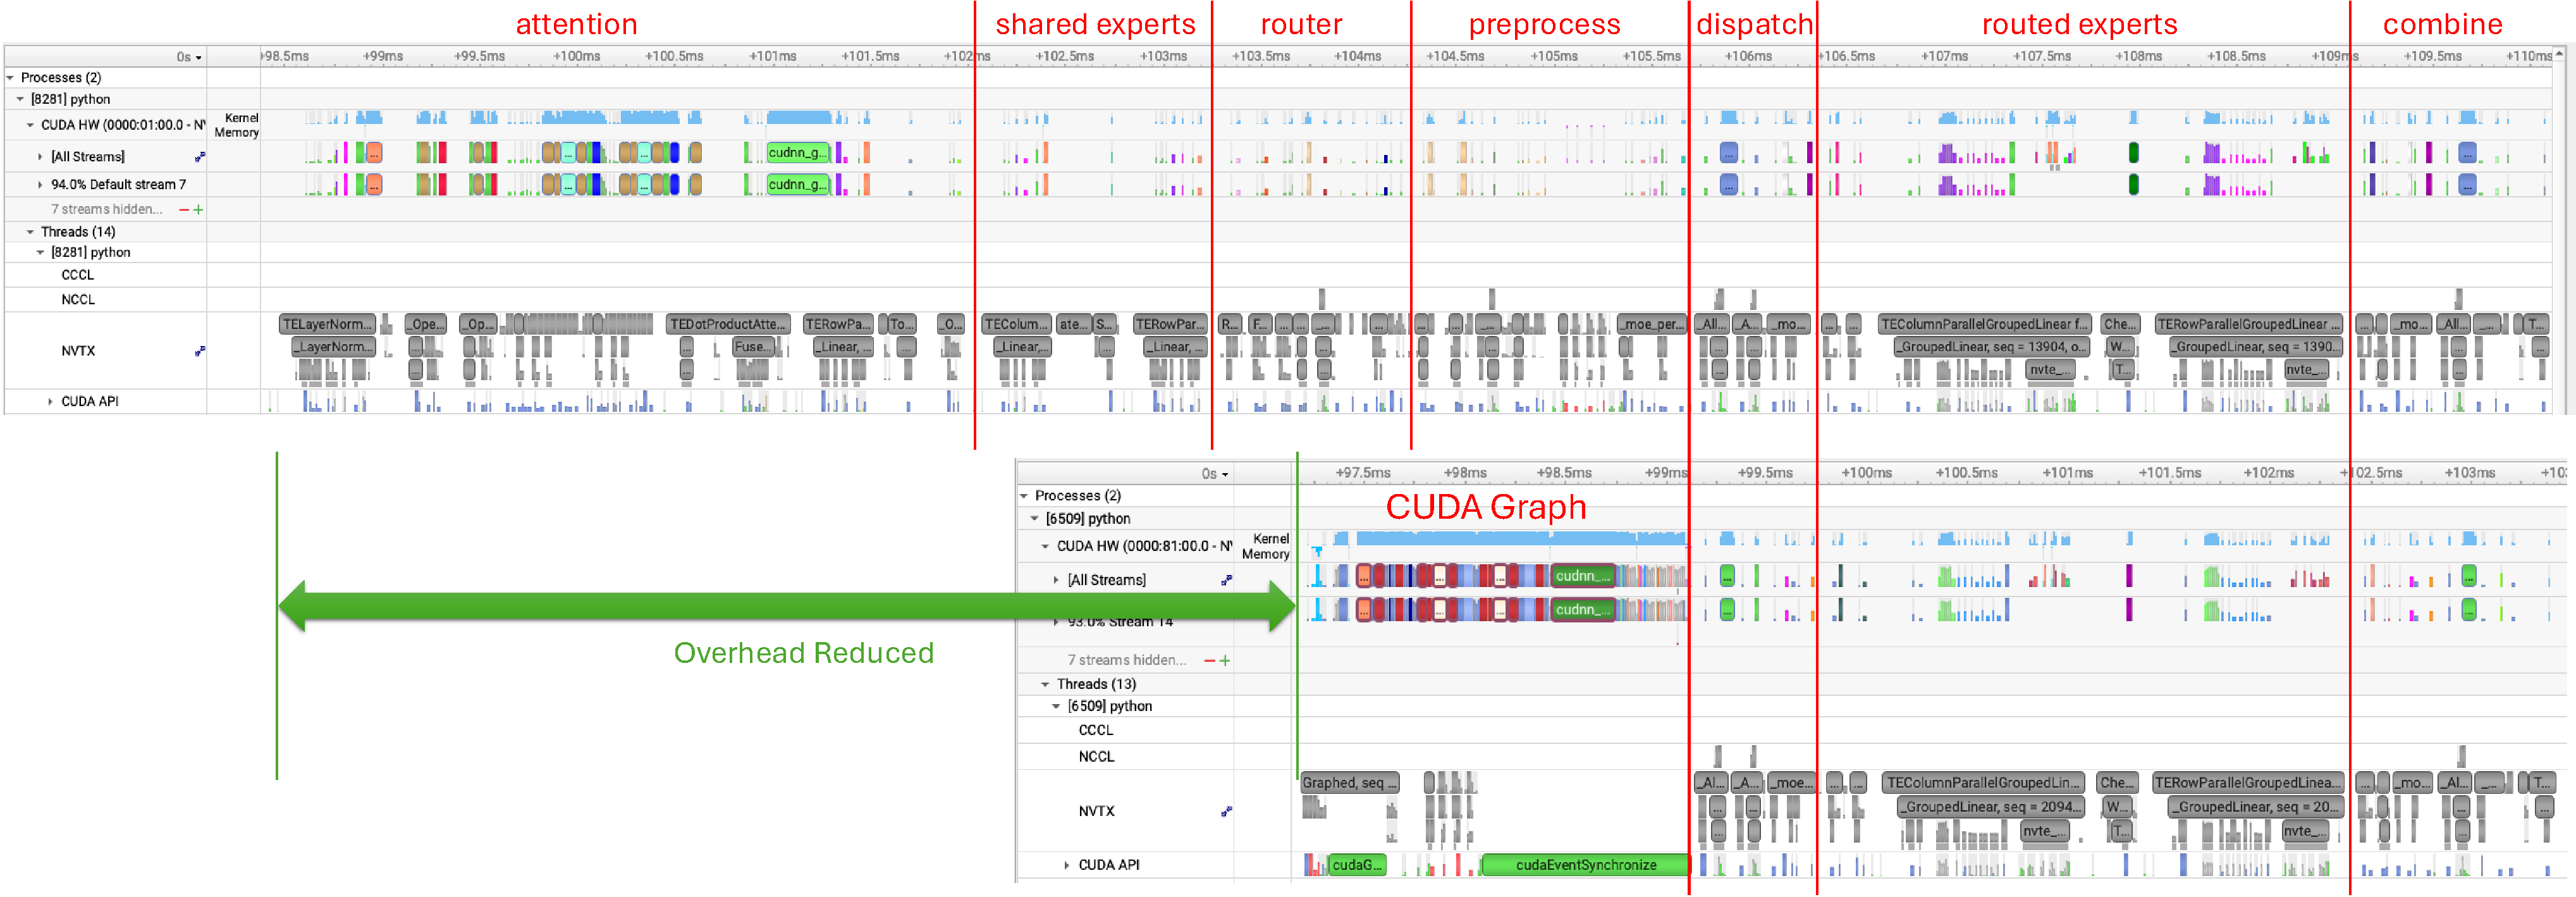
\includegraphics[width=0.95\linewidth]{figures/partial-cudagraph-nsys.pdf}
    \caption{Transformer 层前向传递：不带（上）和带（下）部分 CUDA 图。静态组件的 CPU 开销很大程度上被消除。}
    \label{fig:partial_cudagraph_nsys}
\end{figure}

Megatron-Core 已进行了广泛的调整，以便 CUDA Graph 能够与多令牌预测 (MTP)、EP 通信重叠、细粒度卸载和检查点以及灵活的 PP 布局等关键功能正常工作。启用部分 CUDA 图形的 Nsight Systems 分析显示 CPU 开销大大降低（\figref{fig:partial_cudagraph_nsys}）。剩余的 CPU 开销主要局限于令牌调度和组合操作之间的区域，由于其动态性质，无法用图表表示。见章节~\ref{sec:sync-free-moe} 有关如何通过使整个层可绘制来解决这个剩余瓶颈的更多详细信息。

\paragraph{CUDA 图的内存优化}

CUDA 图形从三个来源增加内存开销：

\begin{enumerate}
    \item \textbf{图结构}：用于存储图拓扑的内存（通常可以忽略不计）。
    \item \textbf{独立的内存池}：图形和非图形操作需要单独的 PyTorch 内存池，不能共享内存。对于部分 CUDA 图形，单个转换器层需要两个池：一个用于图形化工作，一个用于非图形化工作。
    \item \textbf{静态缓冲区}：每个图都需要专用的输入/输出静态缓冲区，一旦分配，就会从 PyTorch 的内存分配器中取出。
\end{enumerate}

如果不仔细优化，部分 CUDA 图形将从上述三个来源产生更高的内存开销。 Megatron-Core 和 Transformer Engine 实施了多项优化来最大限度地减少这种开销：

\textit{减少图表数量。}
具有管道并行性（PP）， \textbf{每个微批次} 需要专用的 CUDA Graph。原因是，如果微批次共享一个图，那么微批次 $i+1$的前向传递将覆盖微批次之前保存的上下文 $i$的向后传递执行，导致内存损坏（\figref{fig:pp-microbatch-graph-sharing}）。这导致 $L \times M \times 2$ 总共的图表（其中 $L$ = 每个 GPU 的层数， $M$ = 微批次， $\times 2$ 用于前进/后退）。

相反，如果不使用 PP，微批次可以共享相同的图，从而将计数减少到 $L \times 2$。要启用图形共享， \texttt{is\_first\_microbatch} 引入 GPU 标志是为了控制共享图中特定于微批次的行为，例如仅在第一个微批次上运行的量化。在重放之前将此标志设置为 0 或 1 会导致根据需要跳过或执行捕获的量化内核。

\begin{figure}[ht]
    \centering
    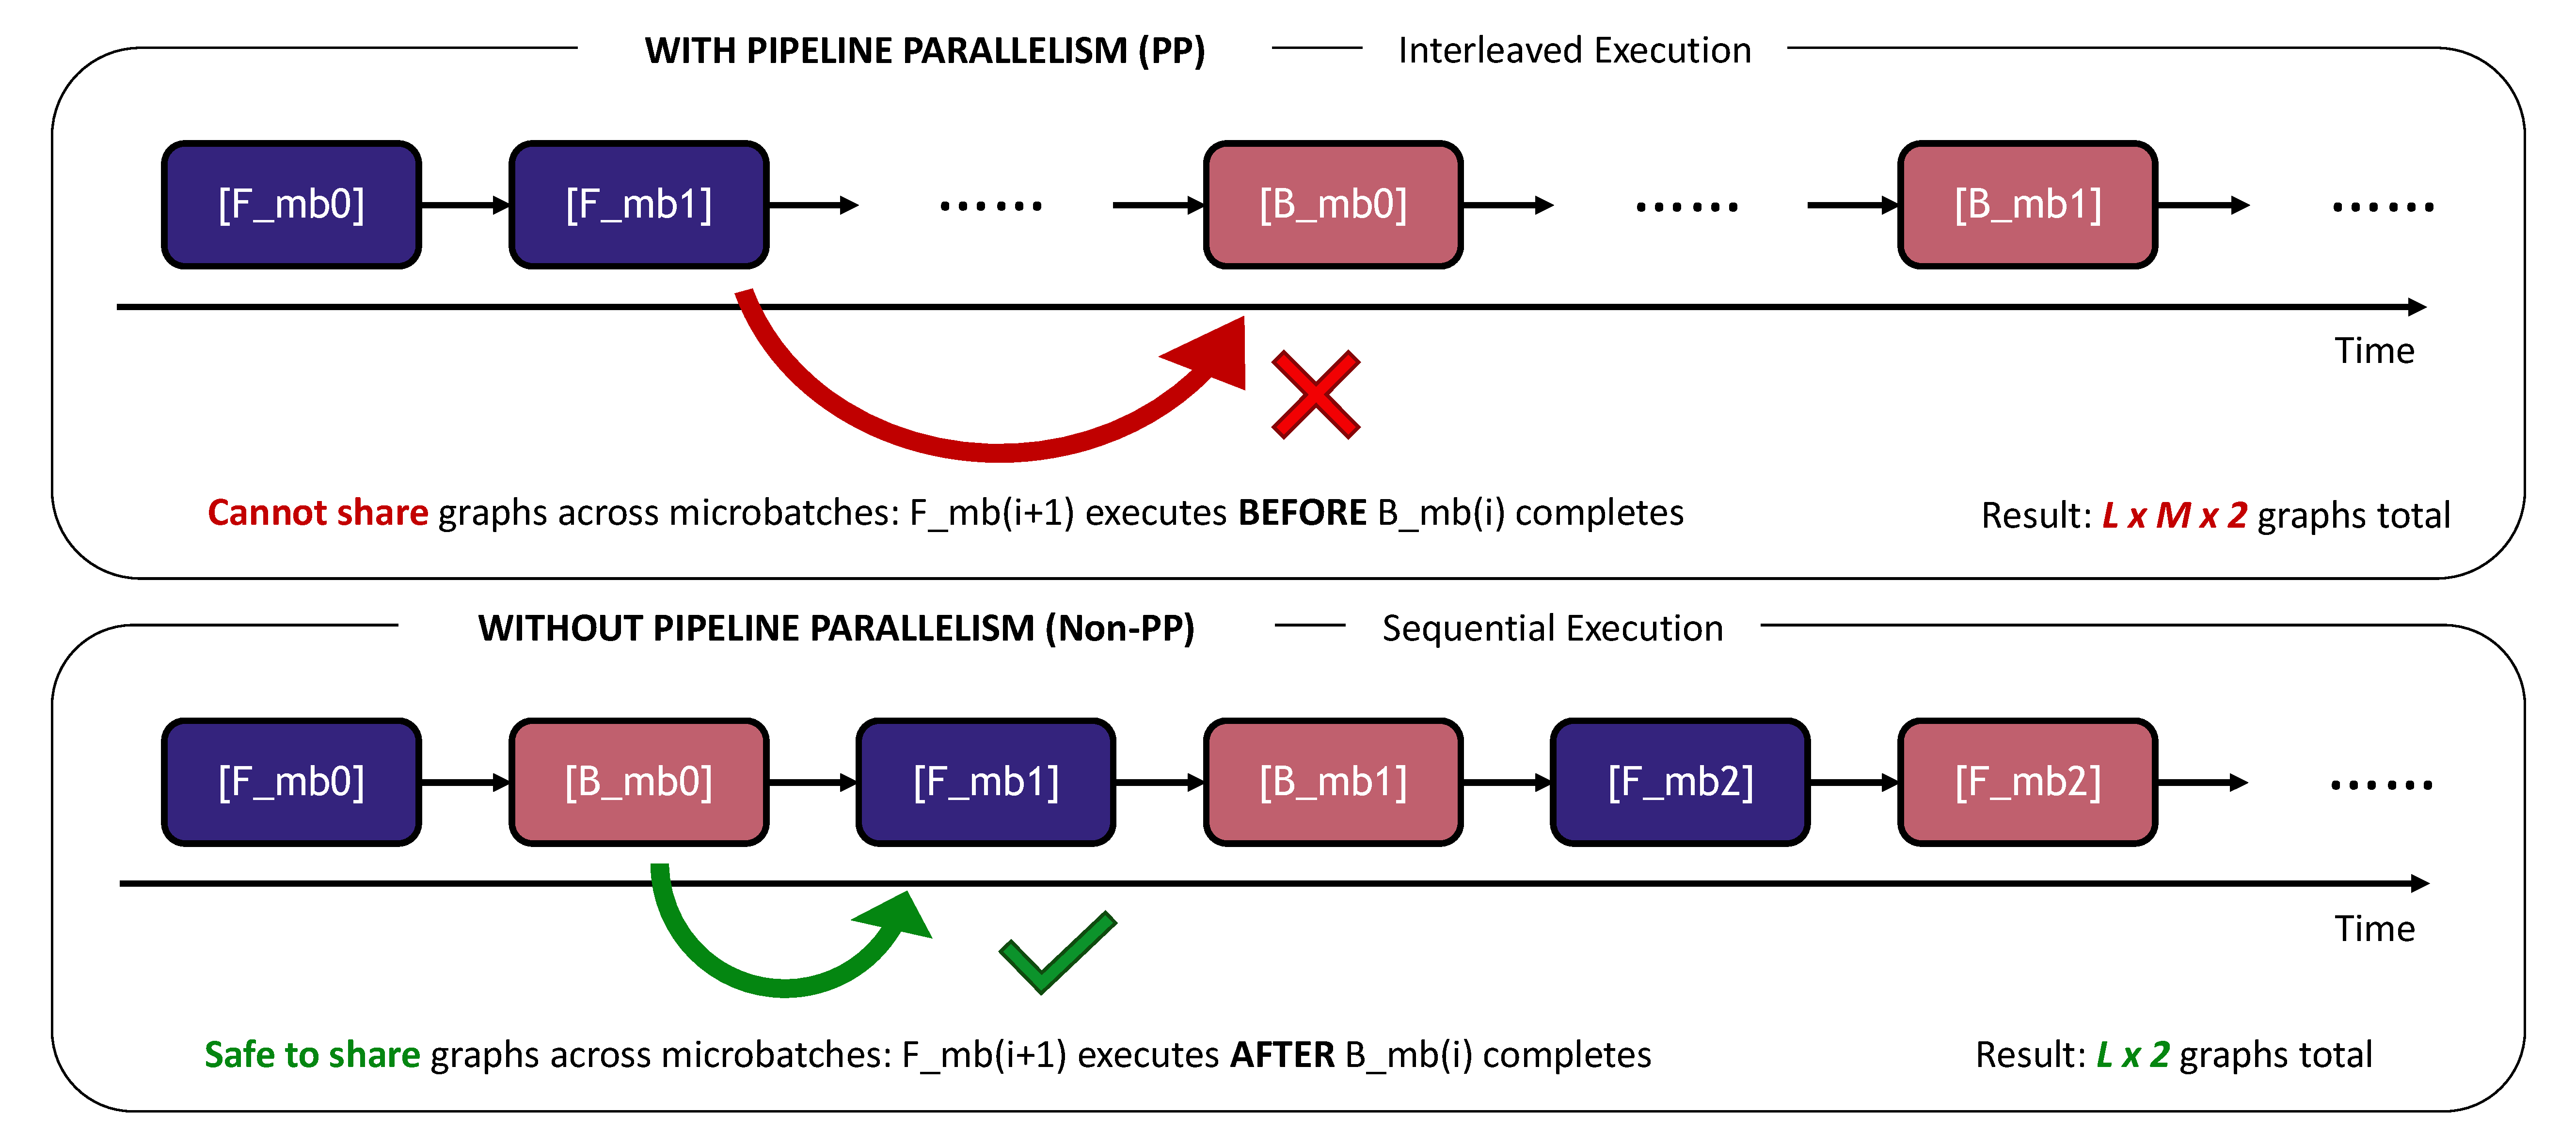
\includegraphics[width=0.9\textwidth]{figures/cudagraph_pp.pdf}
    \caption{为什么管道并行性会阻止 CUDA 图在微批次之间共享。 \textbf{含PP} （上）：执行是交错的——在任何向后传递之前运行多个向前传递。如果微批次共享一个图，F\_mb1 覆盖 F 保存的上下文\_B 之前的 mb0\_mb0 使用它，导致内存损坏。每个微批次都需要自己的图（$L \times M \times 2$ 图表总数）。 \textbf{不含PP} （下）：执行是连续的——每个微批次在下一个微批次开始之前完成（向前+向后）。上下文在被覆盖之前被消耗，因此微批次可以安全地共享图（仅 $L \times 2$ 图表总数）。}
    \label{fig:pp-microbatch-graph-sharing}
\end{figure}

\textit{池共享。}
尽管图形化和非图形化操作需要单独的内存池，但所有图形在按执行顺序捕获时都可以共享一个池。Transformer发动机 \texttt{make\_graphed\_callables()} API 接受 \texttt{\_order} 指定微批次间调度的参数，允许通过正确的池共享进行顺序捕获。

\textit{缓冲区重用。}
静态输入/输出缓冲区可以根据并程执行顺序在图之间重复使用。一旦微批次完成了一层的向后传递，其前向缓冲区和向后输入缓冲区就可供下一个前向和后向图重用。只有后向输出缓冲区必须保留，直到数据发送到下一个 PP 阶段。

通过这些内存优化，我们实现了 10\% 在 DeepSeek-V3 GB200 训练中，通过大约 7~GB 的额外内存实现端到端加速。

\paragraph{剩下的问题：动态专家计算}

完整 CUDA 图形不支持无滴 MoE。部分 CUDA 图形消除了静态组件的 CPU 开销，但是 \textbf{动态专家计算区域保留在图之外}。我们有什么办法可以制作 CUDA 图吗 \textit{覆盖} 动态部分？要实现这一目标，我们至少必须解决两个挑战：
\begin{enumerate}
    \item \textbf{动态形状需要主机-设备同步}：主机必须从 GPU 查询每个专家的令牌计数才能启动令牌调度和分组 GEMM。
    \item \textbf{内存分配需要已知缓冲区大小}：最坏情况的缓冲区分配会浪费内存；实际大小分配需要同步。
\end{enumerate}

下一小节将介绍 Megatron-Core 如何通过三种互补技术（无同步内核、ECHO 和分页存储）实现无滴 MoE 的完整 CUDA 图形覆盖。

\subsubsection{通过无同步内核、ECHO 和分页存储实现 Dropless MoE 的完整 CUDA 图形覆盖}\label{sec:sync-free-moe}

虽然内核融合和 CUDA 图有助于减少主机开销，但无滴 MoE 引入了新的挑战：动态张量形状需要主机设备同步，从而阻止 CUDA 图覆盖专家计算。

在无滴 MoE 中，每个 EP 等级接收的令牌计数根据路由决策动态变化。路由器在 GPU 上生成此形状信息，但主机需要它来启动后续操作并分配内存。获取此信息需要设备到主机的复制和同步，将 CPU 置于关键路径上并防止 CUDA Graph 捕获动态部分。为了通过动态路由实现无同步 MoE 的无丢包训练，存在两个基本挑战：

\textbf{挑战 1：在不知道实际问题大小的情况下启动内核。}
传统上，许多 GPU 操作员假设（动态）形状信息在主机上可用。主机端代码确定启动配置，例如网格大小和图块大小，以及内核必须根据运行时获得的形状信息执行的工作量。在 dropless MoE 中，这会创建一个主机设备同步点：主机必须在启动 Grouped GEMM 或通信内核之前从设备查询每个专家的令牌计数。为了解决这个问题，需要重新设计处理动态形状的 GPU 内核。我们开发了 \textbf{设备启动的 GPU 内核}，包括设备发起的分组 GEMM 和使用 HybridEP 的无同步调度。

\textbf{挑战2：在不知道实际大小的情况下分配内存。}
无同步执行意味着缓冲区的大小需要在主机上预先确定。为了避免令牌溢出，缓冲区通常需要过大，例如，基于最坏情况的大小，以适应所有令牌都路由到同一专家的情况。然而，这种过度配置会导致严重的内存碎片：如果实际的令牌分配是平衡的，则绝大多数预分配的内存仍然未使用，但它无法被图中的其他操作回收。最坏情况下的缓冲区可能需要 $O(\text{EP\_size})$ 内存比实际工作集多出几倍。

这种内存碎片可以通过两种互补的策略来缓解： \emph{减少负载不平衡} 以便最坏情况下的配置更接近实际使用情况，并且 \emph{动态内存管理} 在 CUDA Graph 中回收未使用的缓冲区空间。 \textbf{回声} 采用第一种策略，通过动态克隆未充分利用的排名上的热门专家，减少每个排名令牌计数的差异，从而减少最坏情况和平均内存需求之间的差距。 \textbf{分页存储} 采用第二种策略，在 CUDA Graph 中启用细粒度内存管理，允许将预分配缓冲区的未使用部分重新用于其他操作。 ECHO 和分页存储的详细信息如下。

\paragraph{设备启动的 GPU 内核}
\label{sec:device-init}

为了消除传统主机启动的 GPU 操作符所需的强制主机设备同步，内核必须 \emph{设备发起的}。这需要三件事：
\begin{itemize}
\item[i.] GPU内核需要从GPU内存中读取形状信息并用它来指导计算。
\item[ii.] GPU 内核需要将其执行的实际工作量（仅在运行时才知道）与其静态启动配置解耦。
\item[iii.] GPU内核需要跳过不必要的计算，例如对填充数据的操作。
\end{itemize}
为了满足这些要求，必须重新设计现有内核。下面以 Grouped GEMM 内核和 HybridEP 内核作为两个具体示例。

\textbf{设备发起的分组 GEMM。}
正如章节中所讨论的~\ref{sec:grouped-gemm}TE 提供两种分组 GEMM 实施：多流 cuBLASLt GEMM 和 CUTLASS 分组 GEMM。两者都是主机发起的。它们需要每个专家令牌计数的 CPU 端列表来确定每个 GEMM 的形状和启动配置，从而创建主机设备同步障碍。为了消除这个问题，TE 引入了设备启动的 Grouped GEMM，它直接从设备内存读取形状信息。提供了两种实现方式：

\begin{itemize}
\item[i.] \textbf{cuBLASLt 分组 GEMM。}
从 CUDA 13.1 开始，cuBLASLt Grouped GEMM 支持将矩阵形状作为设备数组传递。此实现包括用于选择最佳内核配置的内置启发式方法，现在涵盖了最新 CUDA 版本中的各种精度和缩放模式。

\item[ii.] \textbf{CuteDSL 分组 GEMM 具有融合激活和量化。}
在基于cuteDSL的实现中，SwiGLU激活可以融合到尾声阶段，对于FP8训练，也可以融合量化。虽然当前的支持仅限于特定的精度和融合模式，但持续的开发不断扩大新配置的覆盖范围。
\end{itemize}

\textbf{使用 HybridEP 进行无同步调度。}
HybridEP，在小节中介绍过~\ref{sec:deepep}，提供了 MoE 通信的高效实现，并且在无同步 MoE 中也发挥着重要作用。在每次调度和排列之后，给定等级接收到的令牌数量是动态的，通常需要同步来获取缓冲区大小。通过估计上限并将其传递给 HybridEP，调度程序可以根据该界限预先分配输出缓冲区，从而以额外 GPU 内存为代价消除所有同步。

即使使用设备启动的内核，最坏情况的缓冲区分配也会浪费内存。两个互补的策略可以解决这个问题： \textbf{回声} 减少负载不平衡，因此最坏情况的配置接近实际使用情况，同时 \textbf{分页存储} 启用细粒度内存管理以回收未使用的缓冲区空间。

\paragraph{ECHO：热门专家的弹性克隆。}\label{sec:echo}\footnote{实施细节： \url{https://github.com/NVIDIA/Megatron-LM/pull/2368}}

负载不平衡是 MoE 固有的：受欢迎的专家比其他人收到更多的令牌，从而产生了两个问题。首先，托管热门专家的 EP 排名成为计算瓶颈，导致其他排名在同步点等待。其次，高负载差异意味着最坏情况下的缓冲区配置与实际使用情况相比会浪费大量内存。 ECHO 通过动态克隆热门专家以在未充分利用的队伍中腾出空位来解决这两个问题。

\figref{fig:echo} 说明了 ECHO 工作流程。在前向传播中，ECHO 规划器识别热门专家并生成两个输出： \emph{热点专家图} 指示哪些专家克隆到哪些空闲插槽，以及更新的 \emph{路线图} 将溢出令牌重定向到克隆。 Expert Dispatch 通过基于 HybridEP 的免同步通信将热专家权重复制到备用插槽；令牌调度将令牌发送给本地专家和克隆专家；专家计算对所有专家进行。在向后传递中，专家梯度调度从克隆中收集梯度并将其简化为家庭专家，以确保一致性。克隆专家在计算后被丢弃以节省内存。

\begin{figure}[ht]
    \centering
    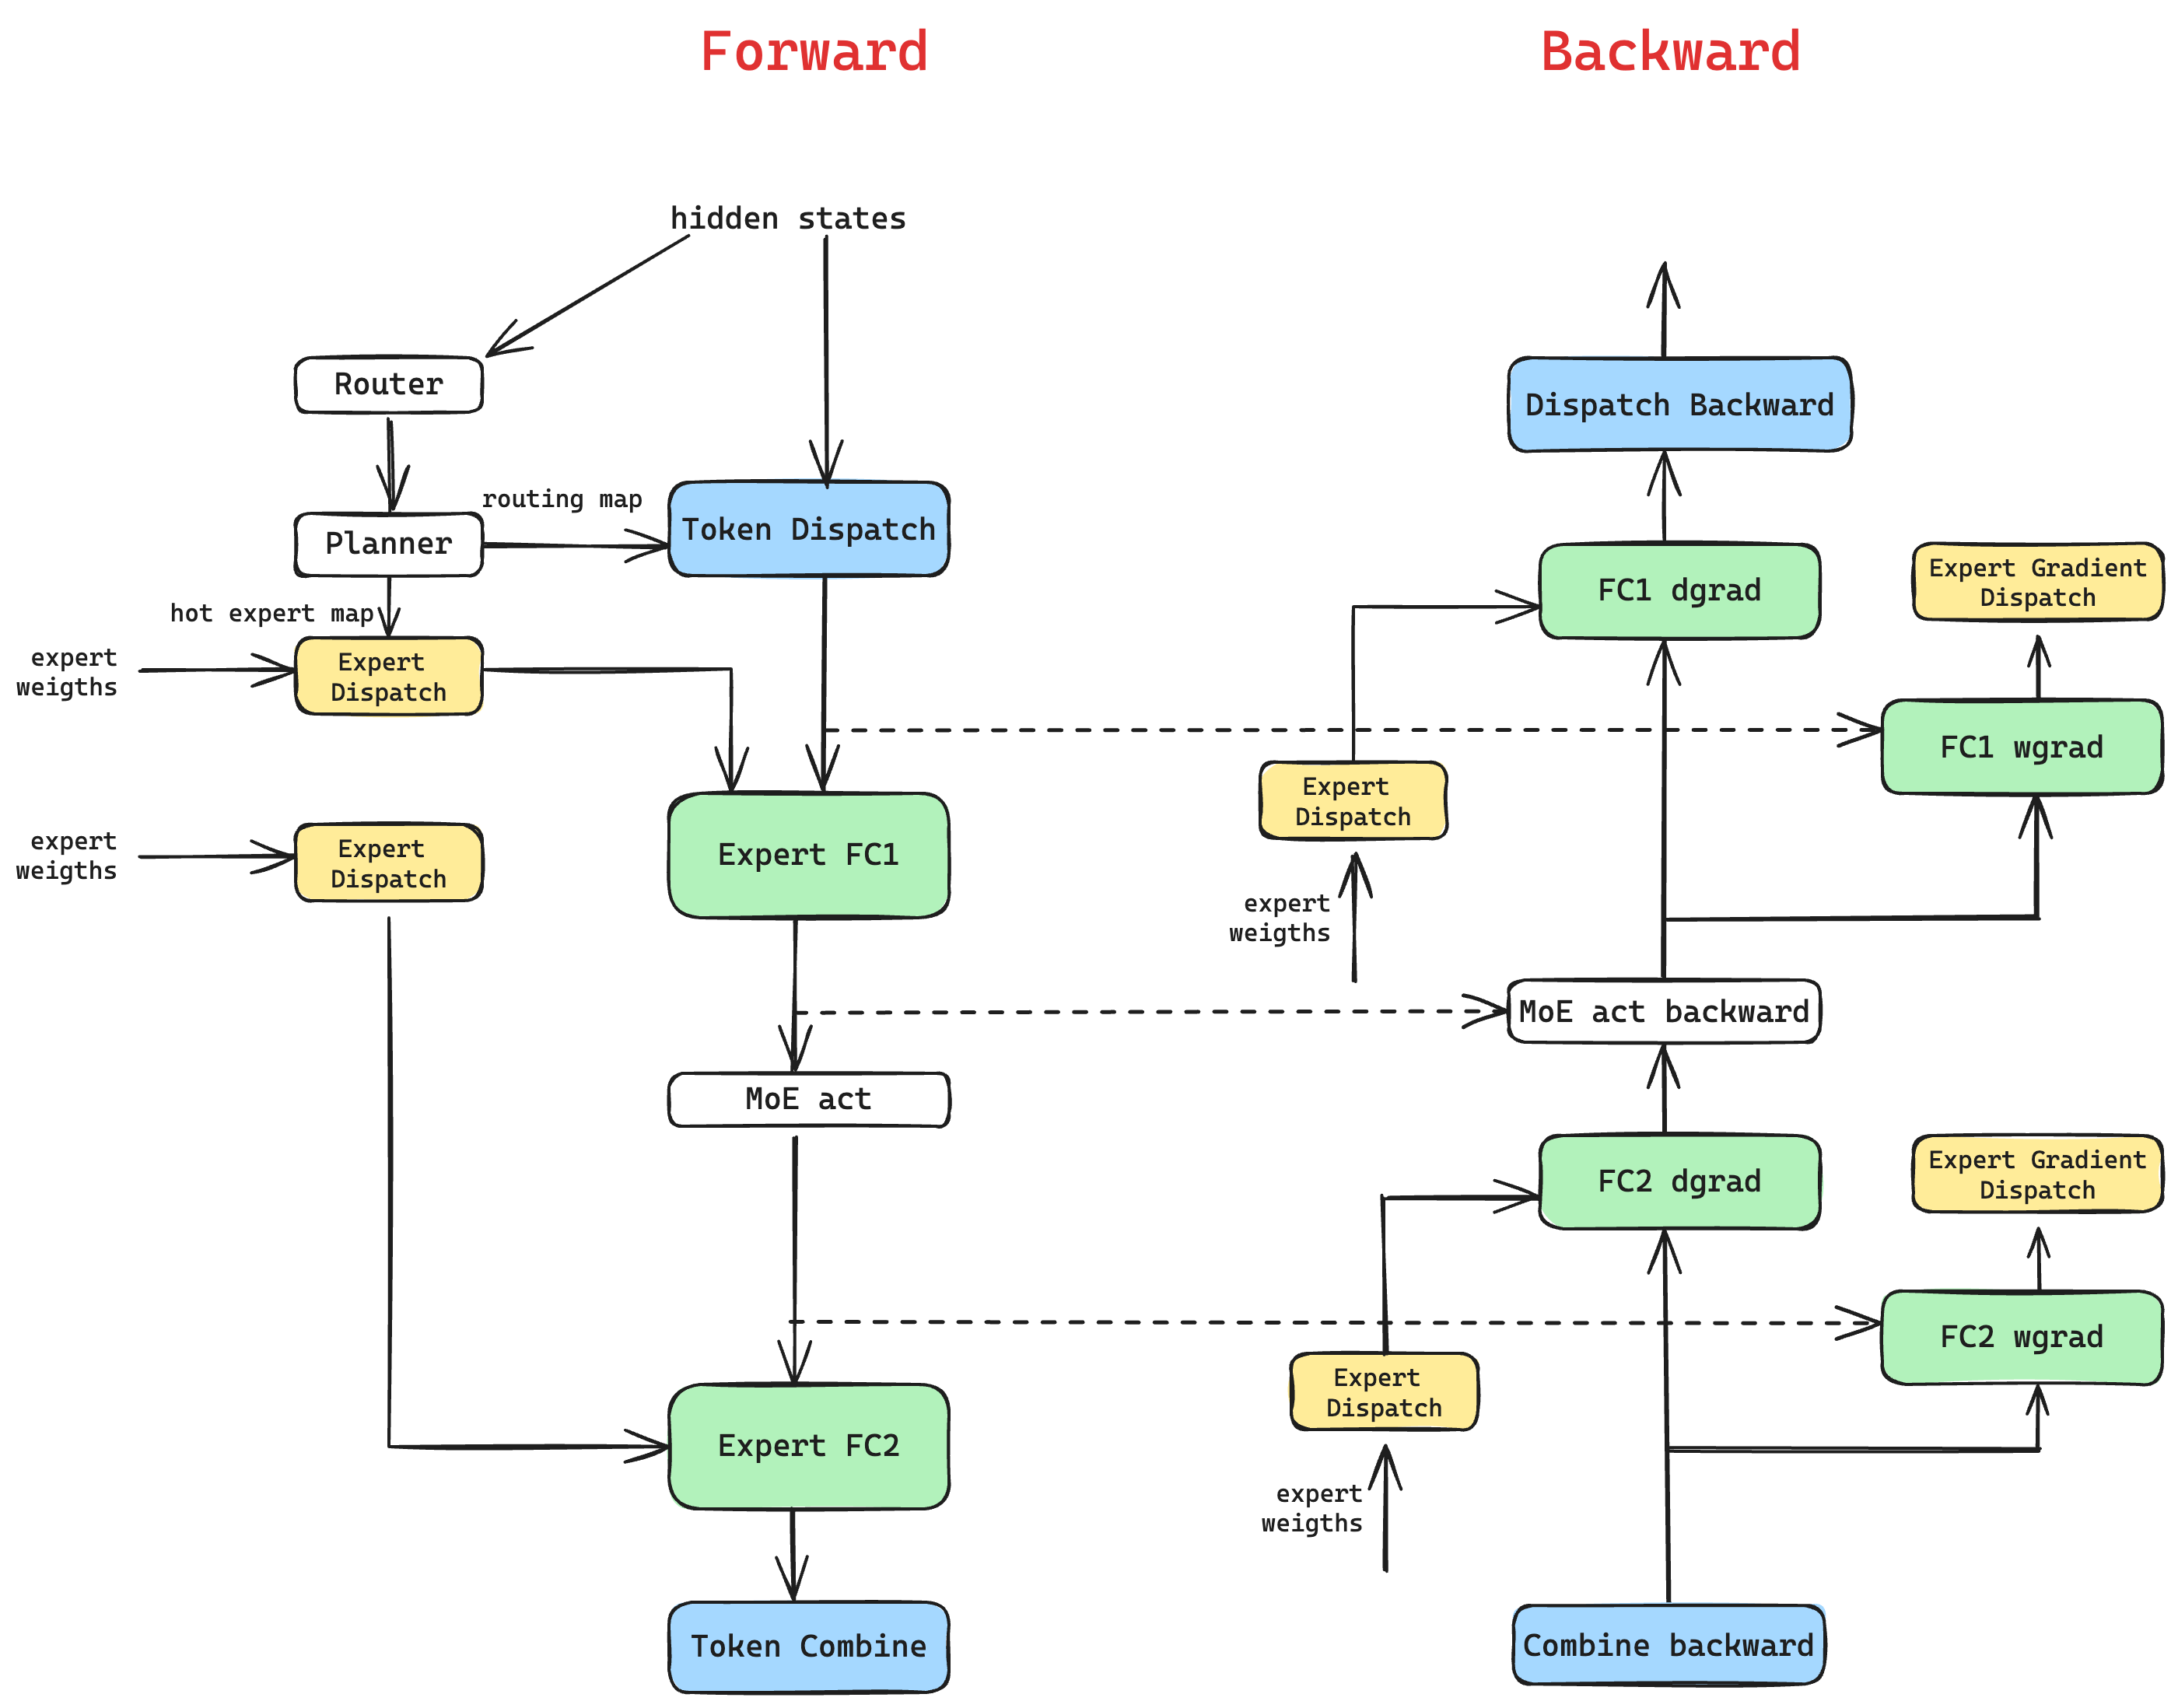
\includegraphics[width=0.85\linewidth]{figures/moe_echo.png}
    \caption{用于向前和向后传递的 ECHO 工作流程。规划器生成路线和热门专家地图。 Expert Dispatch 将热门专家重量复制到备用位置；专家梯度调度可减少梯度返回国内专家。}
    \label{fig:echo}
\end{figure}

克隆专家进行训练比推理要昂贵得多：每个克隆专家都需要在前向过程中进行权重通信，在后向过程中进行梯度减小，以确保一致性。将所有热专家克隆到所有备用插槽可以最大限度地提高负载平衡，但会带来过多的通信开销。 ECHO规划器的目标是最大限度地减少专家克隆的数量，同时实现足够的负载平衡。它计算 \emph{溢出效应} 对于每个专家（超过每个 EP 等级的平均负载的令牌）以及 \emph{闲置产能} 每个等级（可用容量低于平均水平）。使用装箱算法，规划器可以有效地将溢出令牌与备用容量相匹配，确定要克隆哪些特定专家以及克隆到哪个等级，以最小的克隆开销生成热门专家图和路由图。

ECHO 具有两个主要优点：(1) \emph{减少 CUDA 图形的内存碎片}，因为减少 EP 等级之间的负载差异使得最坏情况下的缓冲区大小更接近实际使用情况，从而实现更小的静态缓冲区；和（2） \emph{提高计算效率}，因为平衡的工作负载减少了落后者问题，从而提高了 GPU 的整体利用率。

\paragraph{分页存储。}\footnote{实施细节： \url{https://github.com/NVIDIA/Megatron-LM/pull/2690}}

虽然 ECHO 减少了负载不平衡，以缩小最坏情况和典型内存需求之间的差距，但分页存储解决了补充问题：在 CUDA Graph 中启用细粒度内存管理，以减少内部内存碎片。

碎片问题的出现是因为 CUDA Graph 中涉及的缓冲区大小需要预先确定。为了避免不希望的溢出，缓冲区通常需要过大。在一种简单的方法中，所有层中的缓冲区都根据最坏情况的大小进行分配（\figref{fig:paged_stash}， 中间）。对于无滴 MoE，这意味着每一层根据每个等级可能接收的最大可能令牌保留一个缓冲区，从而导致 $O(\text{layers} \times \text{worst\_case})$ 即使实际令牌计数要低得多，也会产生内存开销。

分页存储基于一个关键的观察：存储向后计算激活所需的实际内存与为避免每层溢出而分配的最坏情况内存之间存在巨大差距（通常超过一个数量级）。分页存储通过解耦这两个内存缓冲区来解决这个问题。这在 \figref{fig:paged_stash} （正确的）。分页存储管理器不是为每一层分配最坏情况大小的缓冲区，而是维护：(1) \emph{临时缓冲区} 调整最坏情况令牌计数的大小，该计数在所有层之间共享以进行计算，以及（2） \emph{隐藏缓冲区} 以页面的形式组织，仅存储每层使用的实际令牌。当一个层完成其前向计算时，其激活值将从 tmp 缓冲区复制到存储缓冲区，仅存储实际令牌计数而不是最坏情况分配。然后，tmp 缓冲区可以轻松地重新用于后续层的计算。这显着减少了内存消耗 $O(\text{layers} \times \text{worst\_case})$ 到 $O(\text{worst\_case} + \text{actual\_total})$.

\begin{figure}[ht]
    \centering
    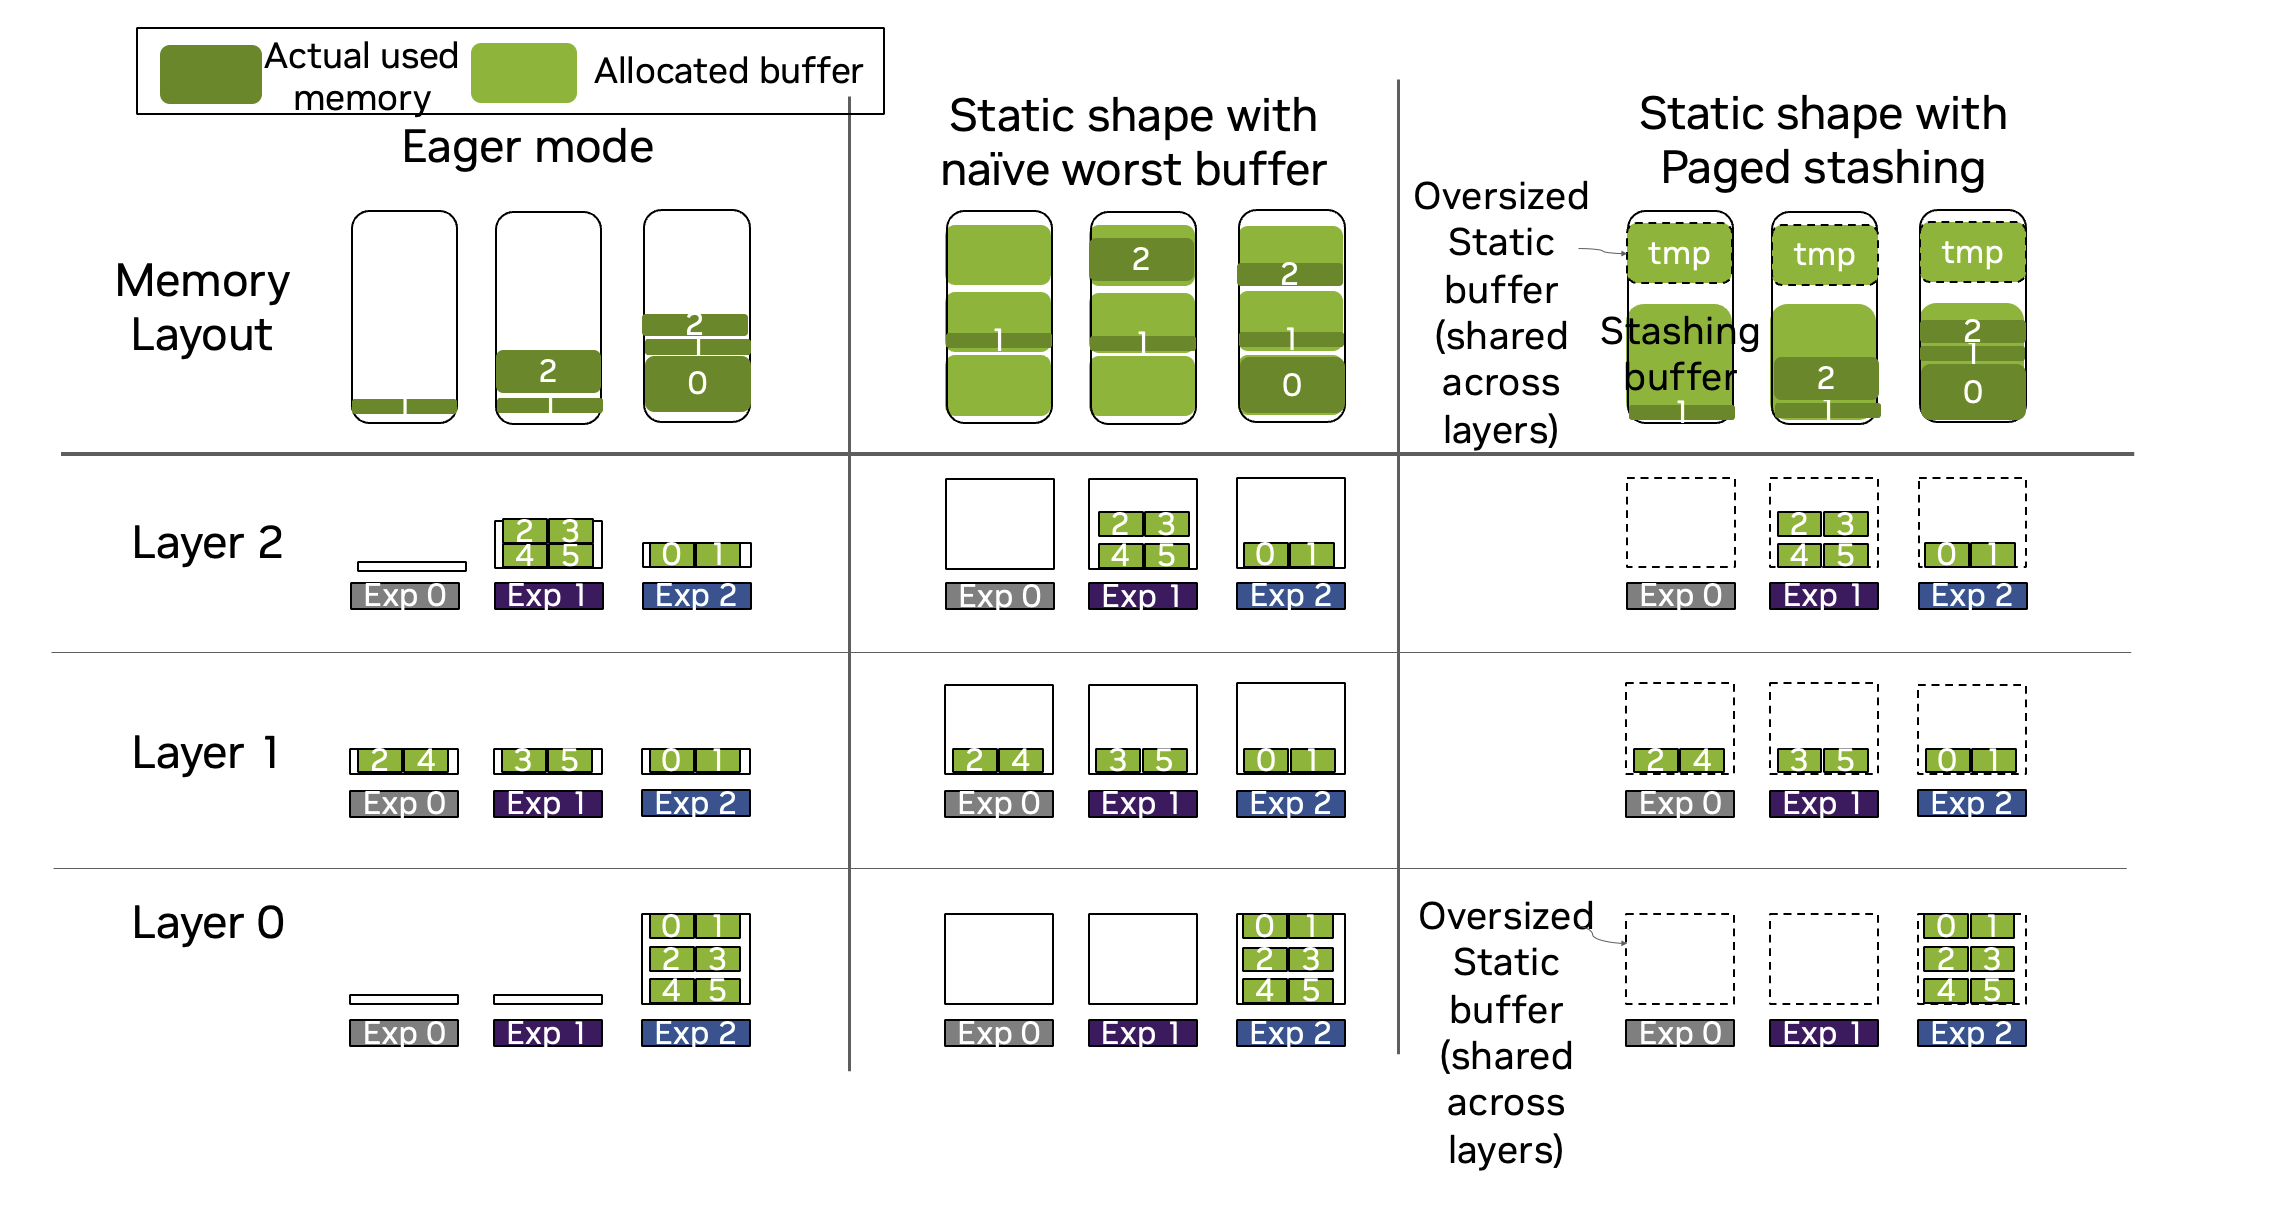
\includegraphics[width=0.95\linewidth]{figures/paged_stash.png}
    \caption{三种执行模式的内存布局比较。 \textbf{左边}：Eager 模式根据实际使用情况动态分配内存。 \textbf{中间}：基线静态形状需要每个层独立地使用最坏情况大小的缓冲区，当实际使用率较低时会导致严重的碎片。 \textbf{正确的}：分页存储使用跨层共享的单个最坏情况 tmp 缓冲区进行计算，而分页存储缓冲区仅存储实际令牌，从而显着减少总内存占用。}
    \label{fig:paged_stash}
\end{figure}

存储缓冲区使用经典的分页思想以灵活而高效的方式管理内存。这 \texttt{PagedStashBuffer} 被组织为固定大小的页面（默认每页 64 个令牌）。页面存储管理器通过循环缓冲区实现的空闲列表来跟踪可用页面。分页操作是由设备启动的 \emph{隐藏内核}。存储内核将激活复制到从空闲列表头部分配的空闲页面并记录目标页面。这 \emph{重新加载内核} 从记录的页面中检索激活并将未使用的页面返回到空闲列表的尾部。

为了最大限度地减少开销，分页存储将内存传输与使用专用 CUDA 流的计算重叠（\figref{fig:paged-stashing-overlap}）。系统在当前计算执行时预取下一个向后层的激活，隐藏重新加载延迟。由于双缓冲，这种重叠需要少量的内存开销。

\begin{figure}[ht]
    \centering
    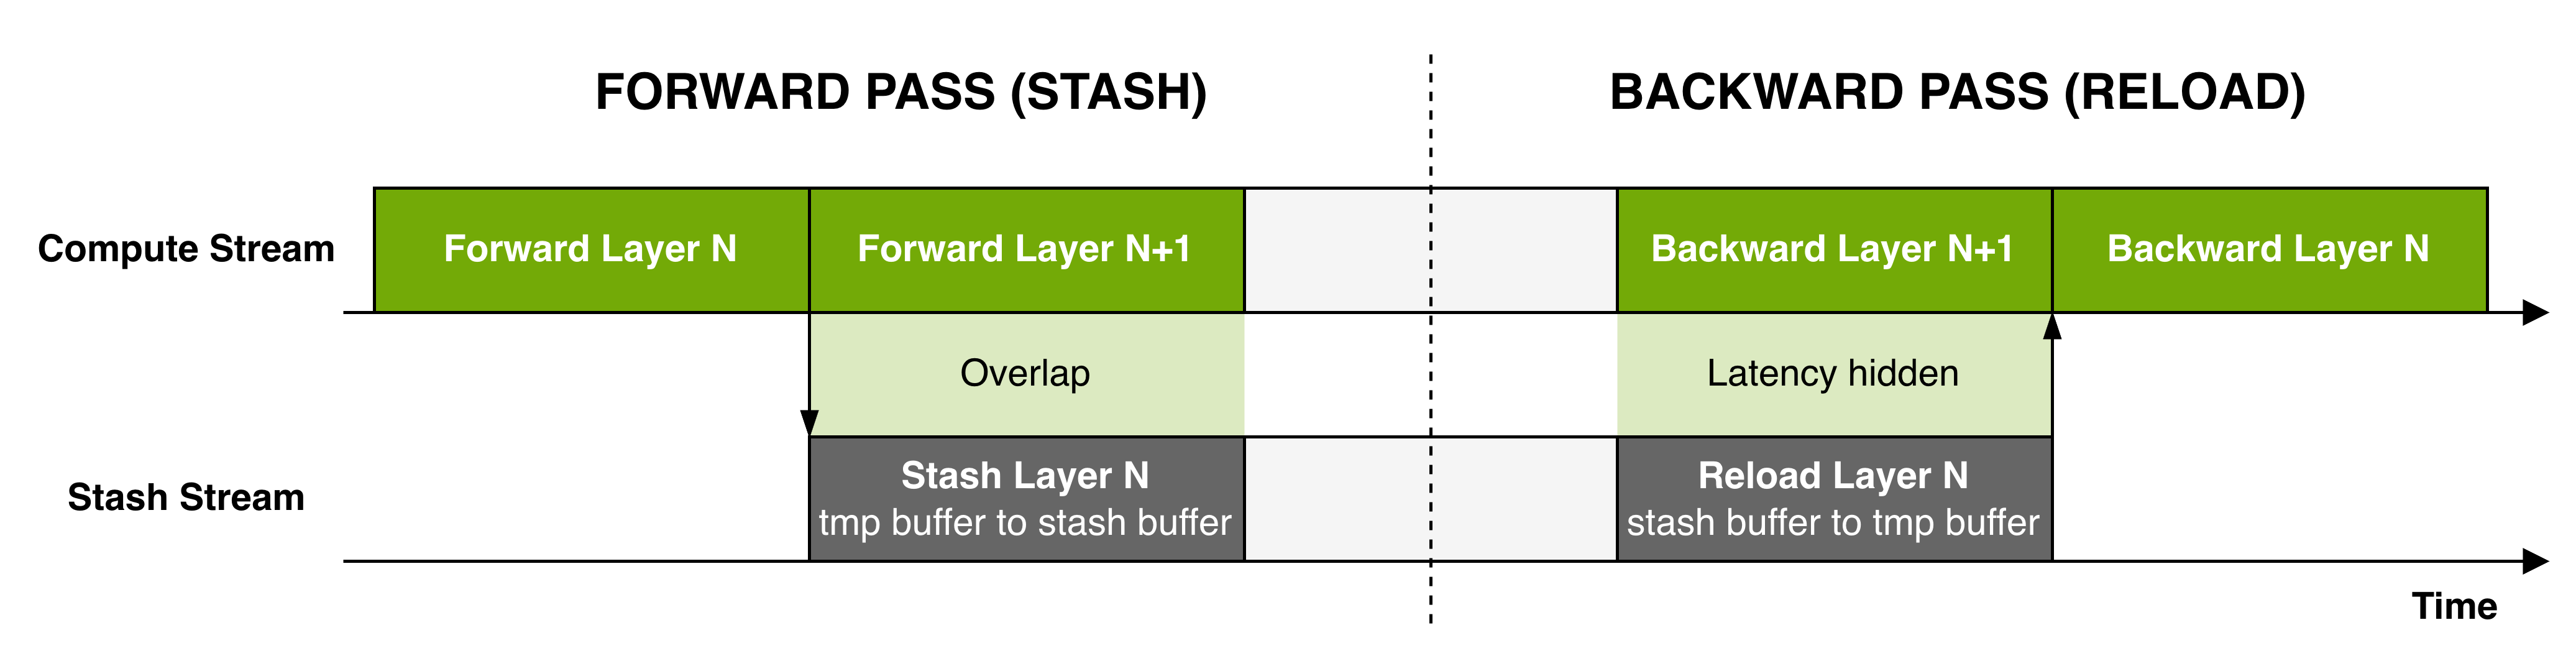
\includegraphics[width=0.9\textwidth]{figures/paged_stashing_overlap.drawio.png}
    \caption{分页存储流重叠。 \textbf{前传}：第 N 层计算后，其激活被存储在专用 Pack 流上（从 tmp 缓冲区复制到分页存储缓冲区），而第 N+1 层在主计算流上计算 — 存储完全重叠。 \textbf{向后传球}：在第 N 层向后启动之前，在 Unpack 流上预取第 N 层的激活（从存储缓冲区重新加载到 tmp 缓冲区），从而隐藏重新加载延迟。}
    \label{fig:paged-stashing-overlap}
\end{figure}

\paragraph{放在一起：完整的 CUDA 图形覆盖}

这三种技术共同实现了无丢弃式 MoE 的完整 CUDA Graph 覆盖，消除了 CPU 开销，同时保留了动态路由的灵活性：
\begin{itemize}
    \item \textbf{设备启动的内核} 通过直接从 GPU 内存读取动态形状来完全消除主机设备同步，从而使 CUDA 图形可以捕获所有 MoE 操作。
    \item \textbf{回声} 平衡 EP 级别的专家工作量，缩小最坏情况和实际缓冲要求之间的差距。这可以实现更小的静态分配，并缓解掉队问题，否则会限制 GPU 利用率。
    \item \textbf{分页存储} 减少记忆 $O(\text{layers} \times \text{worst\_case})$ 到 $O(\text{worst\_case} + \text{actual\_total})$ 通过跨层共享单个最坏情况 tmp 缓冲区并仅将实际激活存储在分页存储缓冲区中。
\end{itemize}

\noindent\textbf{开销。}
这些好处伴随着谨慎的权衡。
ECHO 引入了额外的通信，用于在前向传递中克隆热门专家并在后向传递中减少其梯度；实际上，只有一小部分专家被克隆（由高于平均负载的溢出决定），因此相对于标准的全对全调度，额外的通信仍然是适度的。
分页存储添加了内存复制操作（在前向传递中存储，在后向传递中重新加载）和具有双缓冲开销的持久最坏情况大小的 tmp 缓冲区；这些副本在与层计算重叠的专用 CUDA 流上运行，因此延迟在很大程度上是隐藏的，主要成本是额外的内存带宽。
与消除每次迭代主机设备同步和使用 CUDA 图形实现静态内存规划所带来的收益相比，这两种开销都相对较小。

\subsubsection{概括}

计算效率优化解决了效率低下的两个根源。对于内核效率：分组 GEMM 批处理专家计算，内核融合整合路由和排列操作，降低精度训练可加速 Tensor Core 吞吐量。对于主机开销：CUDA Graph 消除了每次迭代的 CPU 逻辑，Sync-Free MoE 消除了主机设备同步障碍。 ECHO 解决了使这两个问题复杂化的负载不平衡问题。这些优化共同将计算效率低下从主要瓶颈转变为可管理的约束。

\subsection{摘要：打破三堵墙}

本节讨论了MoE高效培训的三个基本障碍，每一个障碍都是硬性约束，如果不解决，就会阻碍大规模的实际培训。

\begin{itemize}
    \item \textbf{内存墙}：内存是第一个限制。如果参数、优化器状态和激活超出 GPU 容量，则训练无法继续。内存高效排列、FP8/FP4 激活、细粒度重新计算、卸载、精度感知优化器和 FSDP 一起将 DeepSeek-V3 的 199.5 GB 每 GPU 要求转换为可行的训练配置。

    \item \textbf{通信墙}：通信开销直接降低了GPU利用率。优化调度程序（DeepEP、HybridEP）最大化带宽，FWD-BWD 重叠隐藏计算背后的延迟。总之，这些措施可将整体开销从多达 60\% 训练时间少于10\% 在 DeepSeek-V3 训练中。

    \item \textbf{计算效率墙}：计算效率低下有两个原因：未充分利用 GPU 资源的小内核，以及导致 GPU 闲置的主机开销。分组GEMM和内核融合提高内核效率； CUDA 图形和无同步 MoE 消除了主机开销。这些将计算效率低下从主要瓶颈转变为可管理的约束。
\end{itemize}

这些优化不是独立的。它们形成了一个连贯的系统，其中一堵墙的解决方案可以启用或增强其他墙的解决方案。降低精度的训练清楚地表明了这一点：它减少了内存（激活）并提高了计算效率（更快的 Tensor Core 操作），同时需要仔细集成以避免引入新的瓶颈（量化内核开销）。

以下各节解决了两个交叉问题：第~\ref{sec:reduced-precision-training} 涵盖 FP8/FP4 中的降低精度训练，同时影响所有三堵墙，以及部分~\ref{sec:long-context-training} 解决长上下文 MoE 训练问题，当注意力主导计算时，这会改变优化平衡。


%==============================================================================
% SECTION 5: Low PRECISION TRAINING - THE FP8 JOURNEY
%==============================================================================

\section{MoE FP8/FP4 的降精度训练}\label{sec:reduced-precision-training}

前面的部分针对三堵墙进行了针对性的优化。降低精度训练是独一无二的：它同时影响内存、通信和计算效率，使其成为值得专门处理的跨领域优化。

混合精度训练一直是高效深度学习的基石，以 BF16 为标准实践 \cite{micikevicius2018mixed,peng2023fp8lmtrainingfp8large,xi2024coat}。 FP8/FP4 中的降低精度训练代表了更激进的一步，将精度从 16 位降低到 8 位甚至 4 位，相应的收益和风险也更大 \cite{micikevicius2022fp8formatsdeeplearning,fishman2025scalingfp8trainingtrilliontoken}。对于 DeepSeek-V3，FP8 训练将每个 GPU 的激活内存减少了大约 16 GB，通过更快的 Tensor Core 操作改进了专家 GEMM，并加速了参数 AllGather 通信。这些收益在三堵墙之间复合，使得 FP8 对于高效的大规模 MoE 训练至关重要。

然而，低精度训练会带来收敛风险，必须系统地解决。本节介绍 Megatron-Core 的降低精度训练方法：了解精度的重要性，选择适当的量化方案，以及实施 MoE 特定的优化，以获取降低精度训练的优势，同时保持训练稳定性。

\subsection{为什么低精度训练对MoE很重要}\label{sec:precision-anatomy}

与密集模型相比，MoE 架构放大了低精度训练的好处和风险：

\textbf{扩大效益。} 有了数百名专家，激活记忆就会成比例地扩展。 FP8/FP4 激活比密集模型提供更大的绝对内存节省。参数 AllGather 的通信量减半\footnote{对于 Blackwell 上的 NVFP4 配方，由于我们需要收集行向和列向权重张量，因此节省的通信量也是 50\%.}，而专家 GEMM（主导 MoE 计算）受益于更快的 Tensor Core 吞吐量。

\textbf{风险放大。} 路由器决策取决于精确的分数来将令牌分配给专家。量化噪声可能会破坏专家选择的稳定性，导致训练不稳定、模型质量下降或专家崩溃 \cite{nagel2021whitepaper}。必须保护数字敏感组件免受过度量化。

\textbf{策略：选择性精准。} 解决方案在重要的地方是精确的，在其他地方是效率的。指导MoE部署降低精度训练的三个原则：
\begin{enumerate}
    \item \textbf{保护路由决策。} 路由器仍为FP32，以确保稳定的专家选择。
    \item \textbf{保持关键部件的精度。} 嵌入、输出层、主梯度、主权重和优化器状态保持原始精度以保持模型质量。
    \item \textbf{量化批量计算。} 专家 GEMM 构成了大部分计算，使用经过精心设计的量化方案（称为 \textit{食谱}).
\end{enumerate}

\begin{notebox}
成功降低精度的 MoE 训练的关键是选择性精度：将数值敏感组件（路由器、嵌入、输出层、梯度和优化器状态）保持在更高的精度，同时积极量化大量计算（专家 GEMM）。该策略获得了降低精度训练的大部分好处，同时避免了收敛问题。
\end{notebox}

\subsection{降低精度训练对所有三堵墙的影响}

降低精度训练为所有三个性能墙提供了优势，使其成为统一的优化。表~\ref{tab:fp8-impact-summary} 总结了这些影响。

\begin{table}[ht]
\centering
\begin{threeparttable}
\caption{降低精度训练对三堵墙的影响摘要。}
\label{tab:fp8-impact-summary}
\begin{tabular}{lll}
\toprule
\textbf{墙} & \textbf{降低精度训练的好处} & \textbf{细节} \\
\midrule
记忆 & 50\% (FP8)/75\% (FP4) 活化减少 & 部分~\ref{sec:fp8-activation} \\
        & 消除BF16重量副本 & 部分~\ref{subsec:fp8-primary-weights} \\
        & BF16 优化器状态 & 部分~\ref{sec:precision-opt} \\
\midrule
通信 & 50\% 参数全部收集 \tnote{1} & 部分~\ref{subsec:fp8-primary-weights} \\
\midrule
计算 & 更快的张量核心 GEMM & 部分~\ref{sec:fp8-training} \\
        & 量化内核开销 & 部分~\ref{sec:kernel-fusion} \\
\bottomrule
\end{tabular}
\begin{tablenotes}
    \footnotesize
    \item[1] 对于NVFP4，我们需要同时收集行方向和列方向的FP4权重，因此参数AllGather减少的流量也是50\%.
\end{tablenotes}
\end{threeparttable}
\end{table}

\subsubsection{通过降低精度的训练打破内存墙}

降低精度训练通过三种方式减少内存消耗：

\textbf{激活记忆（详见章节~\ref{sec:fp8-activation}).} 激活内存节省的主要来源来自为向后计算而保存的线性层的输入张量。通过将这些张量存储在 FP8/FP4 而不是 BF16 中，内存占用量减少了 50\%/75\%。例如，FP8 为 DeepSeek-V3 的每个 GPU 节省了大约 16 GB 的激活内存。

\textbf{参数记忆。} 传统的降低精度训练维护三个参数副本：FP32 主权重、BF16 模型权重和 FP8/FP4 计算权重。我们的 \emph{原生 FP8/FP4} 方法（详见第~\ref{subsec:fp8-primary-weights} 下面）通过将权重直接从 FP32 铸造到 FP8/FP4 并以降低的精度执行参数 AllGather 来消除 BF16 副本。

\textbf{优化器状态内存（详见章节~\ref{sec:precision-opt}).} Adam 优化器状态（第一和第二时刻）可以存储在 BF16 而不是 FP32 中，从而将优化器内存减少 50\%。这与降低精度的训练正交，也适用于 BF16。

\subsubsection{通过降低精度的训练打破通信障碍}
\label{sec:comm_wall_quantized_training}

% \textbf{FP8 EP Dispatch (detailed in Section~\ref{sec:fp8-dispatch-comm}).} For fine-grained MoE models with large EP sizes, all-to-all communication becomes a primary bottleneck. By dispatching tokens in FP8 instead of BF16, the communication volume is halved. The key challenge is managing the dequantization-quantization cycle required because forward and backward passes use different quantization dimensions.

\textbf{FP8/FP4 中的参数 AllGather。} 当使用带有分布式优化器的 FP8/FP4 主权重时，参数 AllGather 通信减少 50\% （每个参数 1 个字节与 2 个字节）。注意
\begin{itemize}
    \item 对于NVFP4，我们需要同时收集行方向和列方向的FP4权重，因此参数AllGather减少的流量也是50\%.
    \item 对于 MXFP8，即使使用 FP8 主权重，我们也首先将 FP32 主权重复制到临时 BF16 缓冲区中，并以 BF16 精度进行通信。这是因为 MXFP8 需要向前和向后传递不同的量化方向。通信 MXFP8 权重需要行式和列式量化版本，每个参数有效地通信两个字节，并且消除了与 BF16 通信相比的任何优势。因此，对于 MXFP8，我们以 BF16 精度传递参数。 
\end{itemize}

\subsubsection{通过降低精度的训练打破计算效率壁垒}

\textbf{更快的 GEMM。} FP8（Ada/Hopper 及更高版本）和 FP4（Blackwell 及更高版本）Tensor Core 提供比 BF16 更高的吞吐量，加速前向和后向传递。

\textbf{权衡：量化开销。} 降低精度的训练引入了额外的量化内核，从而增加了 CPU 开销，这对于细粒度 MoE 来说尤其成问题，因为许多小操作已经给 CPU 带来了压力。该开销通过以下方式管理：
\begin{itemize}
    \item \textbf{内核融合} 将量化与其他操作融合在一起，例如标准化和激活函数。
    \item \textbf{熔丝填充/取消填充} 使用排列内核或路由映射来避免显式填充/取消填充。
    \item \textbf{分组量化} 它将多个输入张量的量化融合到一个内核中。
    \item \textbf{CUDA 图形} 捕获量化内核以消除启动开销。见章节~\ref{sec:cuda-graphs} 了解更多详情。
\end{itemize}

\subsection{降低精度训练方案：每张量 FP8、Blockwise FP8、MXFP8 和 NVFP4}

在确定了降低精度训练对所有三面墙的影响后，我们现在检查定义降低精度训练配置的技术组件。

\begin{figure}[ht]
    \centering
    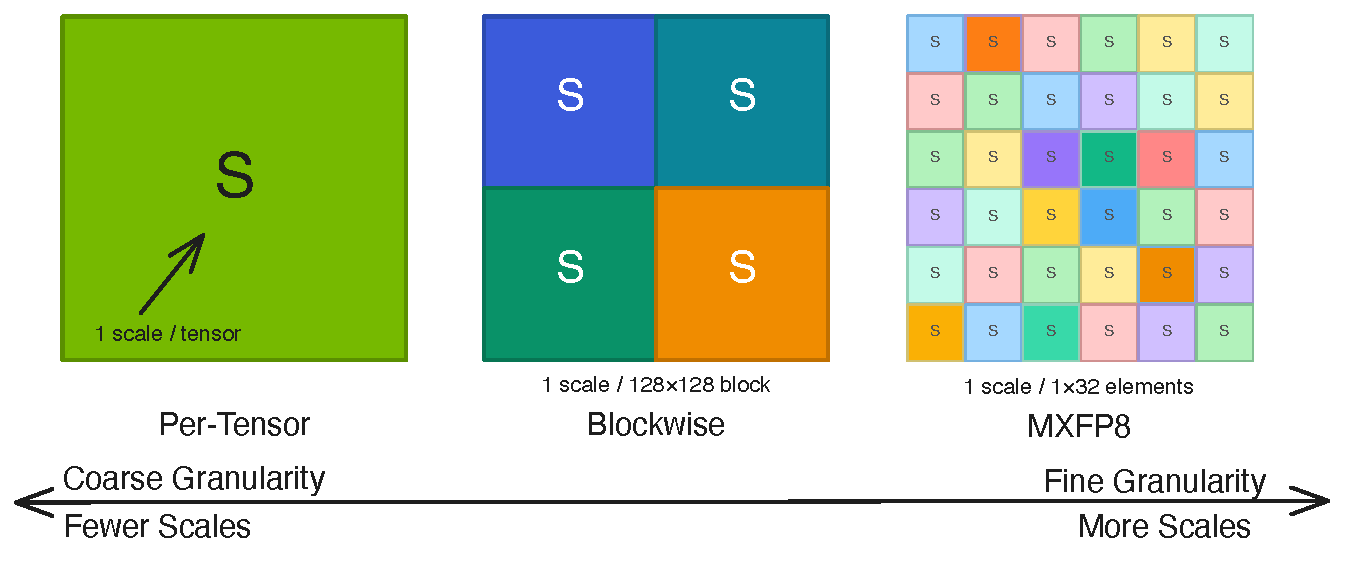
\includegraphics[width=0.9\textwidth]{figures/plots/fp8_recipes_comparison_draft.pdf}
    \caption{FP8 训练方法：每张量缩放、Blockwise FP8 和 MXFP8。}
    \label{fig:fp8-recipes-overview}
\end{figure}

降低精度的训练方法包括：
\begin{itemize}
    \item \textbf{数据格式。} FP8格式有两种：E4M3和E5M2 \cite{micikevicius2022fp8formatsdeeplearning,kuzmin2022fp8quantization}。通常在训练中使用两种组合：
    \begin{itemize}
        \item \textbf{E4M3}：输入、权重和梯度均以 E4M3 格式量化。
        \item \textbf{杂交种}：输入和权重在 E4M3 中量化，而梯度在 E5M2 中量化。
    \end{itemize}
    而对于 FP4，E2M1 是唯一支持的格式。
    \item \textbf{缩放粒度。} 选项包括每个张量和每个块（也称为组或图块）。对于每块缩放，块大小也因配方而异。
    \item \textbf{哪些部分被量化。} 通常所有线性层都会被量化，同时保持嵌入、输出层（LM头）和优化器的原始高精度。部分通信可以采用 FP8/FP4（例如 TP AllGather、DP AllGather、EP all-to-all）。当前降低精度的训练方案通常将 SDPA 保留在 BF16 中。
    \item \textbf{附加机制}，例如随机舍入、随机 Hadamard 变换 (RHT) 等。这些机制是特定于配方的，需要仔细验证。 
\end{itemize}

Megatron-Core 提供了三种 FP8 配方，每种配方均经过大规模验证（\figref{fig:fp8-recipes-overview}）。从按张量到按块再到 MXFP8 的演变反映了硬件进步和大规模部署的经验教训。 \textbf{每张量缩放} 每个张量使用单个比例因子，简单但精度有限，适合实验。 \textbf{块式 FP8} (128$\times$128 个块）提供更细的粒度，并具有经过验证的规模稳定性，推荐用于 Hopper。 \textbf{MXFP8} (1$\times$32 粒度）提供原生 Blackwell Tensor Core 支持和硬件加速缩放（推荐用于 Blackwell）。此外，Megatron-Core还提供了NVFP4配方 \cite{nvidia2025pretraininglargelanguagemodels} 在布莱克威尔。

\subsubsection{每张量 FP8 配方}
Hopper 和 Blackwell 支持的每张量 FP8 配方通常采用混合格式（E4M3 用于输入/权重，E5M2 用于梯度）。它计算输入张量中所有值的绝对最大值 (amax)，并使用该值将张量量化为 FP8。

每个张量缩放有两种变体：
\begin{itemize}
    \item \textbf{延迟缩放}：从历史窗口使用 amax。这打破了 amax 计算和缩放之间的数据依赖性，提供了最佳性能，但存在由于估计的 amax 而损失精度的风险。
    \item \textbf{当前（实时）缩放}：及时计算 amax，提供更好的精度。
\end{itemize}

我们不建议因精度问题而延迟缩放；电流缩放提供了更好的精度和模型收敛性。
人物～\ref{fig:fp8-cs-hopper} 还有~\ref{fig:fp8-cs-blackwell} 分别说明了 Hopper 和 Blackwell 平台上具有每张量电流缩放的线性层的计算。由于 Hopper 仅支持 TN 布局 FP8 GEMM，因此我们必须存储转置的 FP8 激活以用于向后计算。在 Transformer Engine 中，量化内核将转换和转置融合到单个内核中，以减少全局内存访问。在Blackwell平台上，所有布局的FP8 GEMM都受支持，因此我们不需要转置版本，进一步减少了内存占用。

由于其简单性以及相对较好的精度和性能，每张量缩放是迁移到 FP8 训练的良好起点。


\begin{figure*}[t!]
    \centering
    \begin{subfigure}[t]{0.45\textwidth}
        \centering
        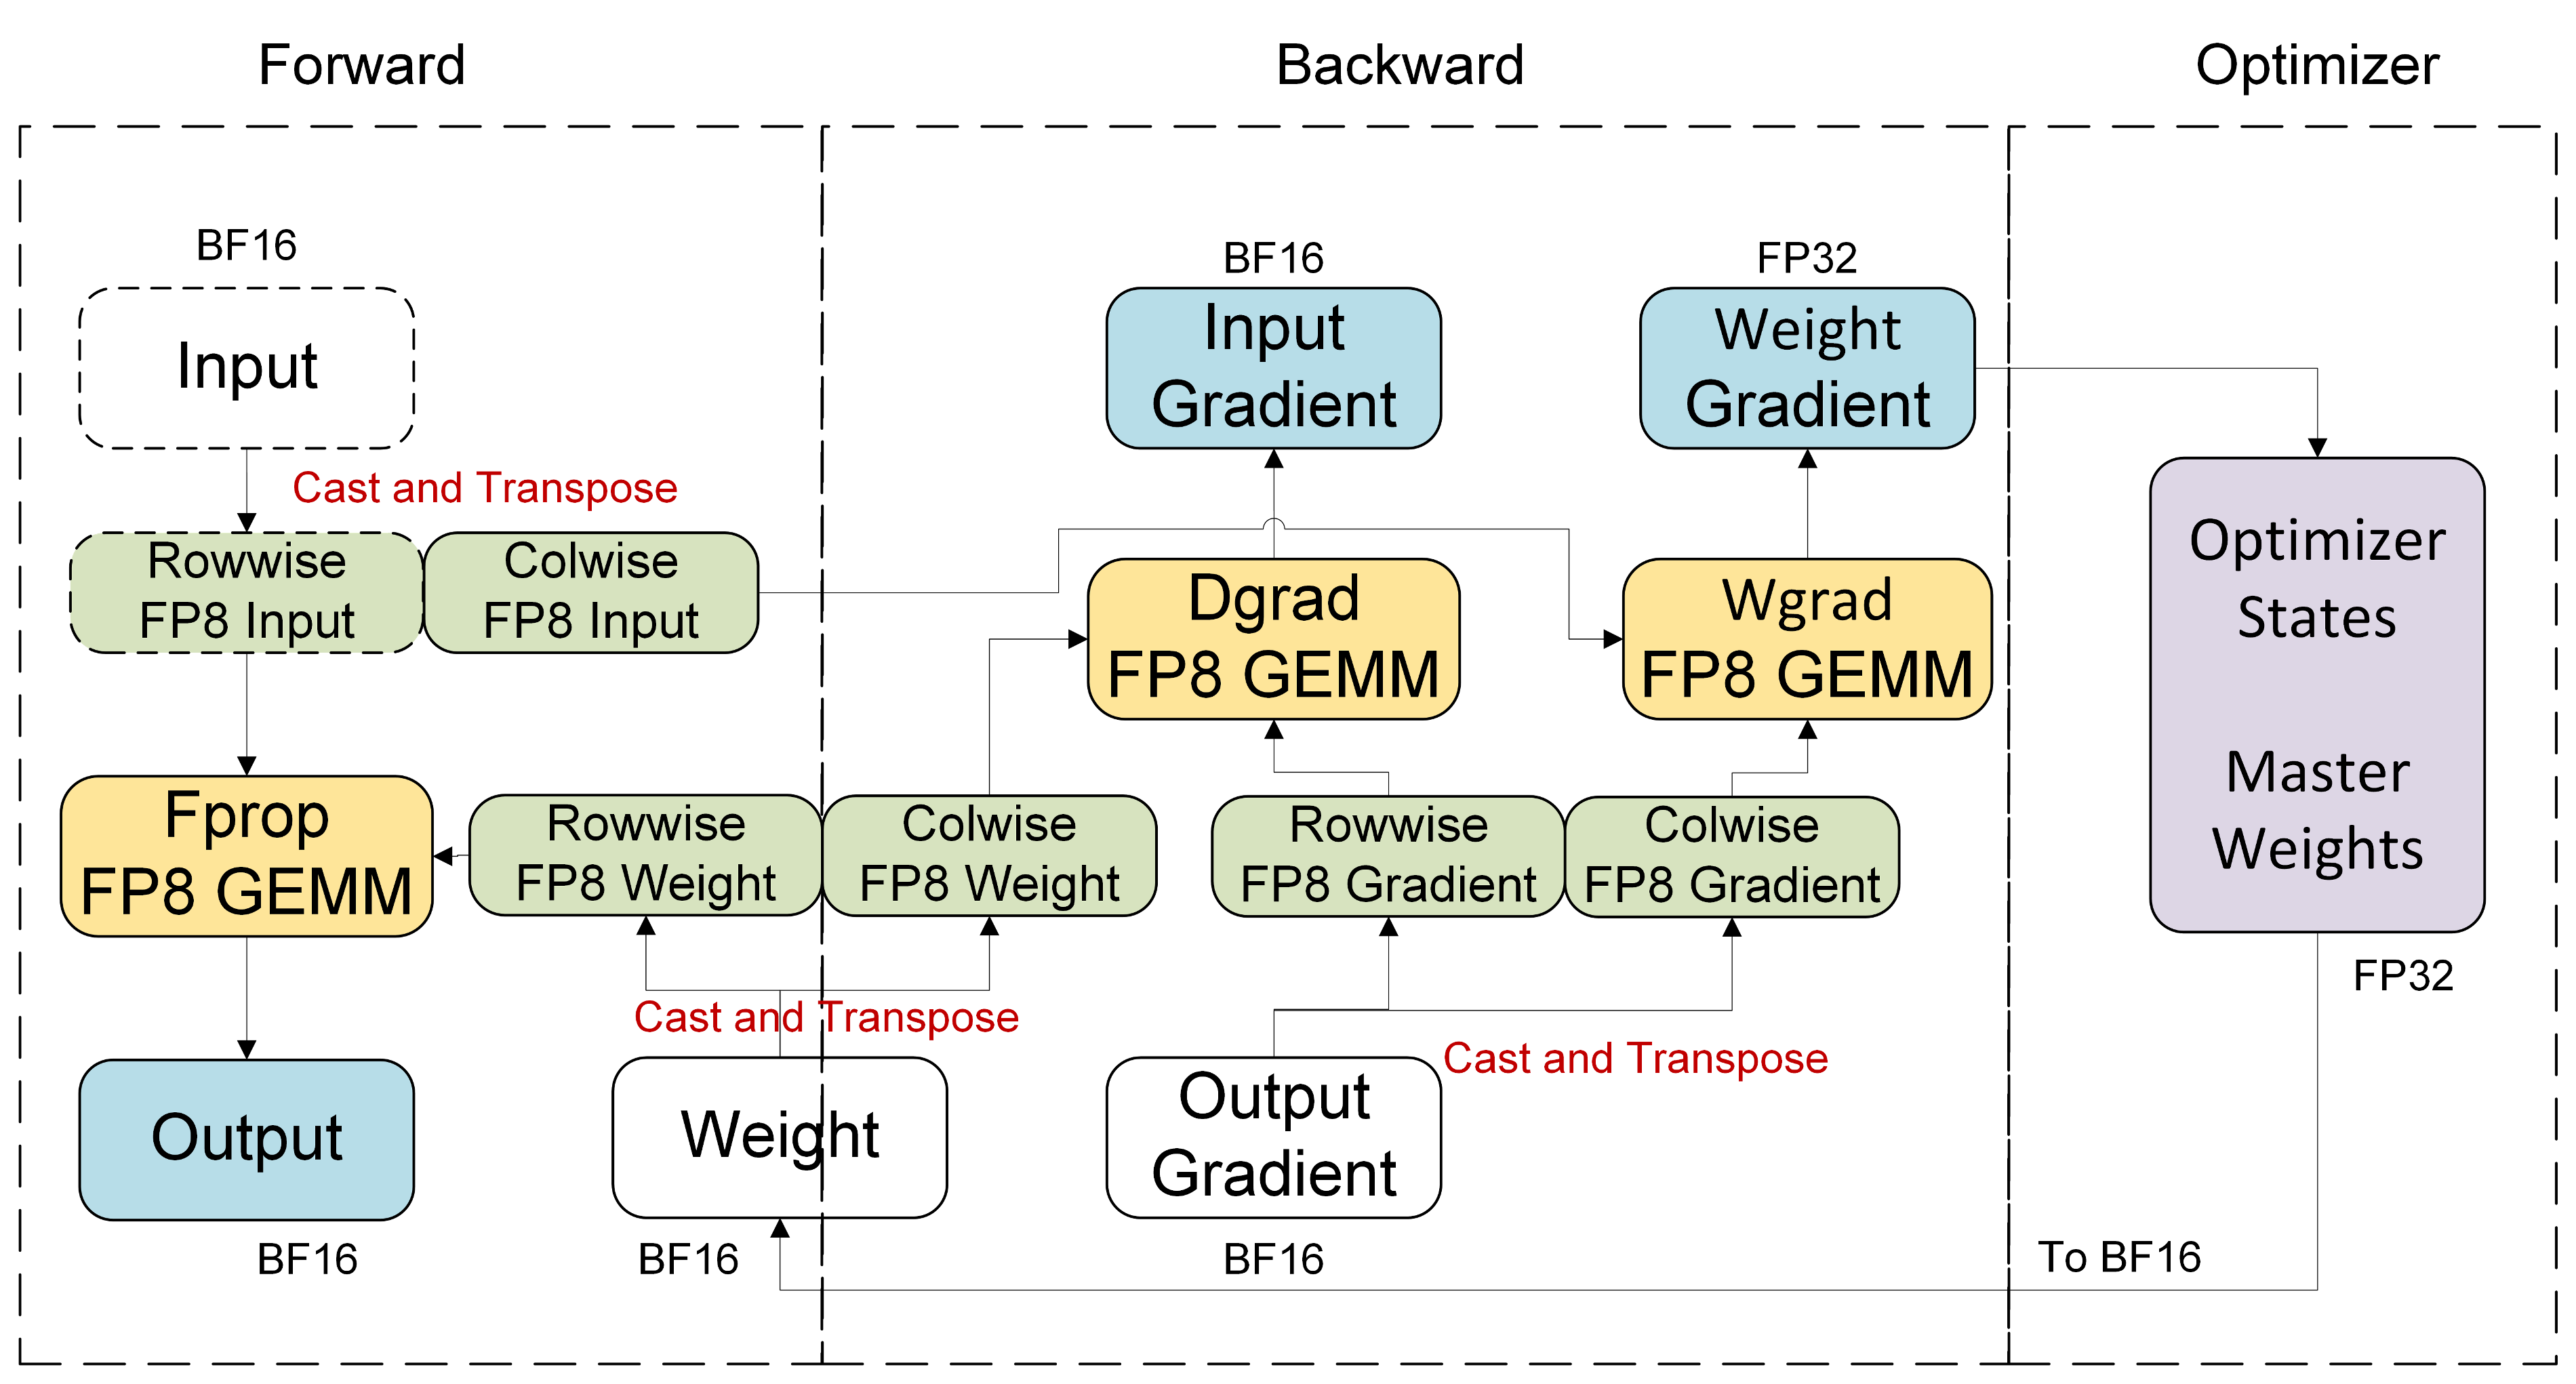
\includegraphics[width=1.0\linewidth]{figures/fp8-cs-hopper.png}
        \caption{Hopper 平台上每个张量的电流缩放。}
        \label{fig:fp8-cs-hopper}
    \end{subfigure}
    \begin{subfigure}[t]{0.45\textwidth}
        \centering
        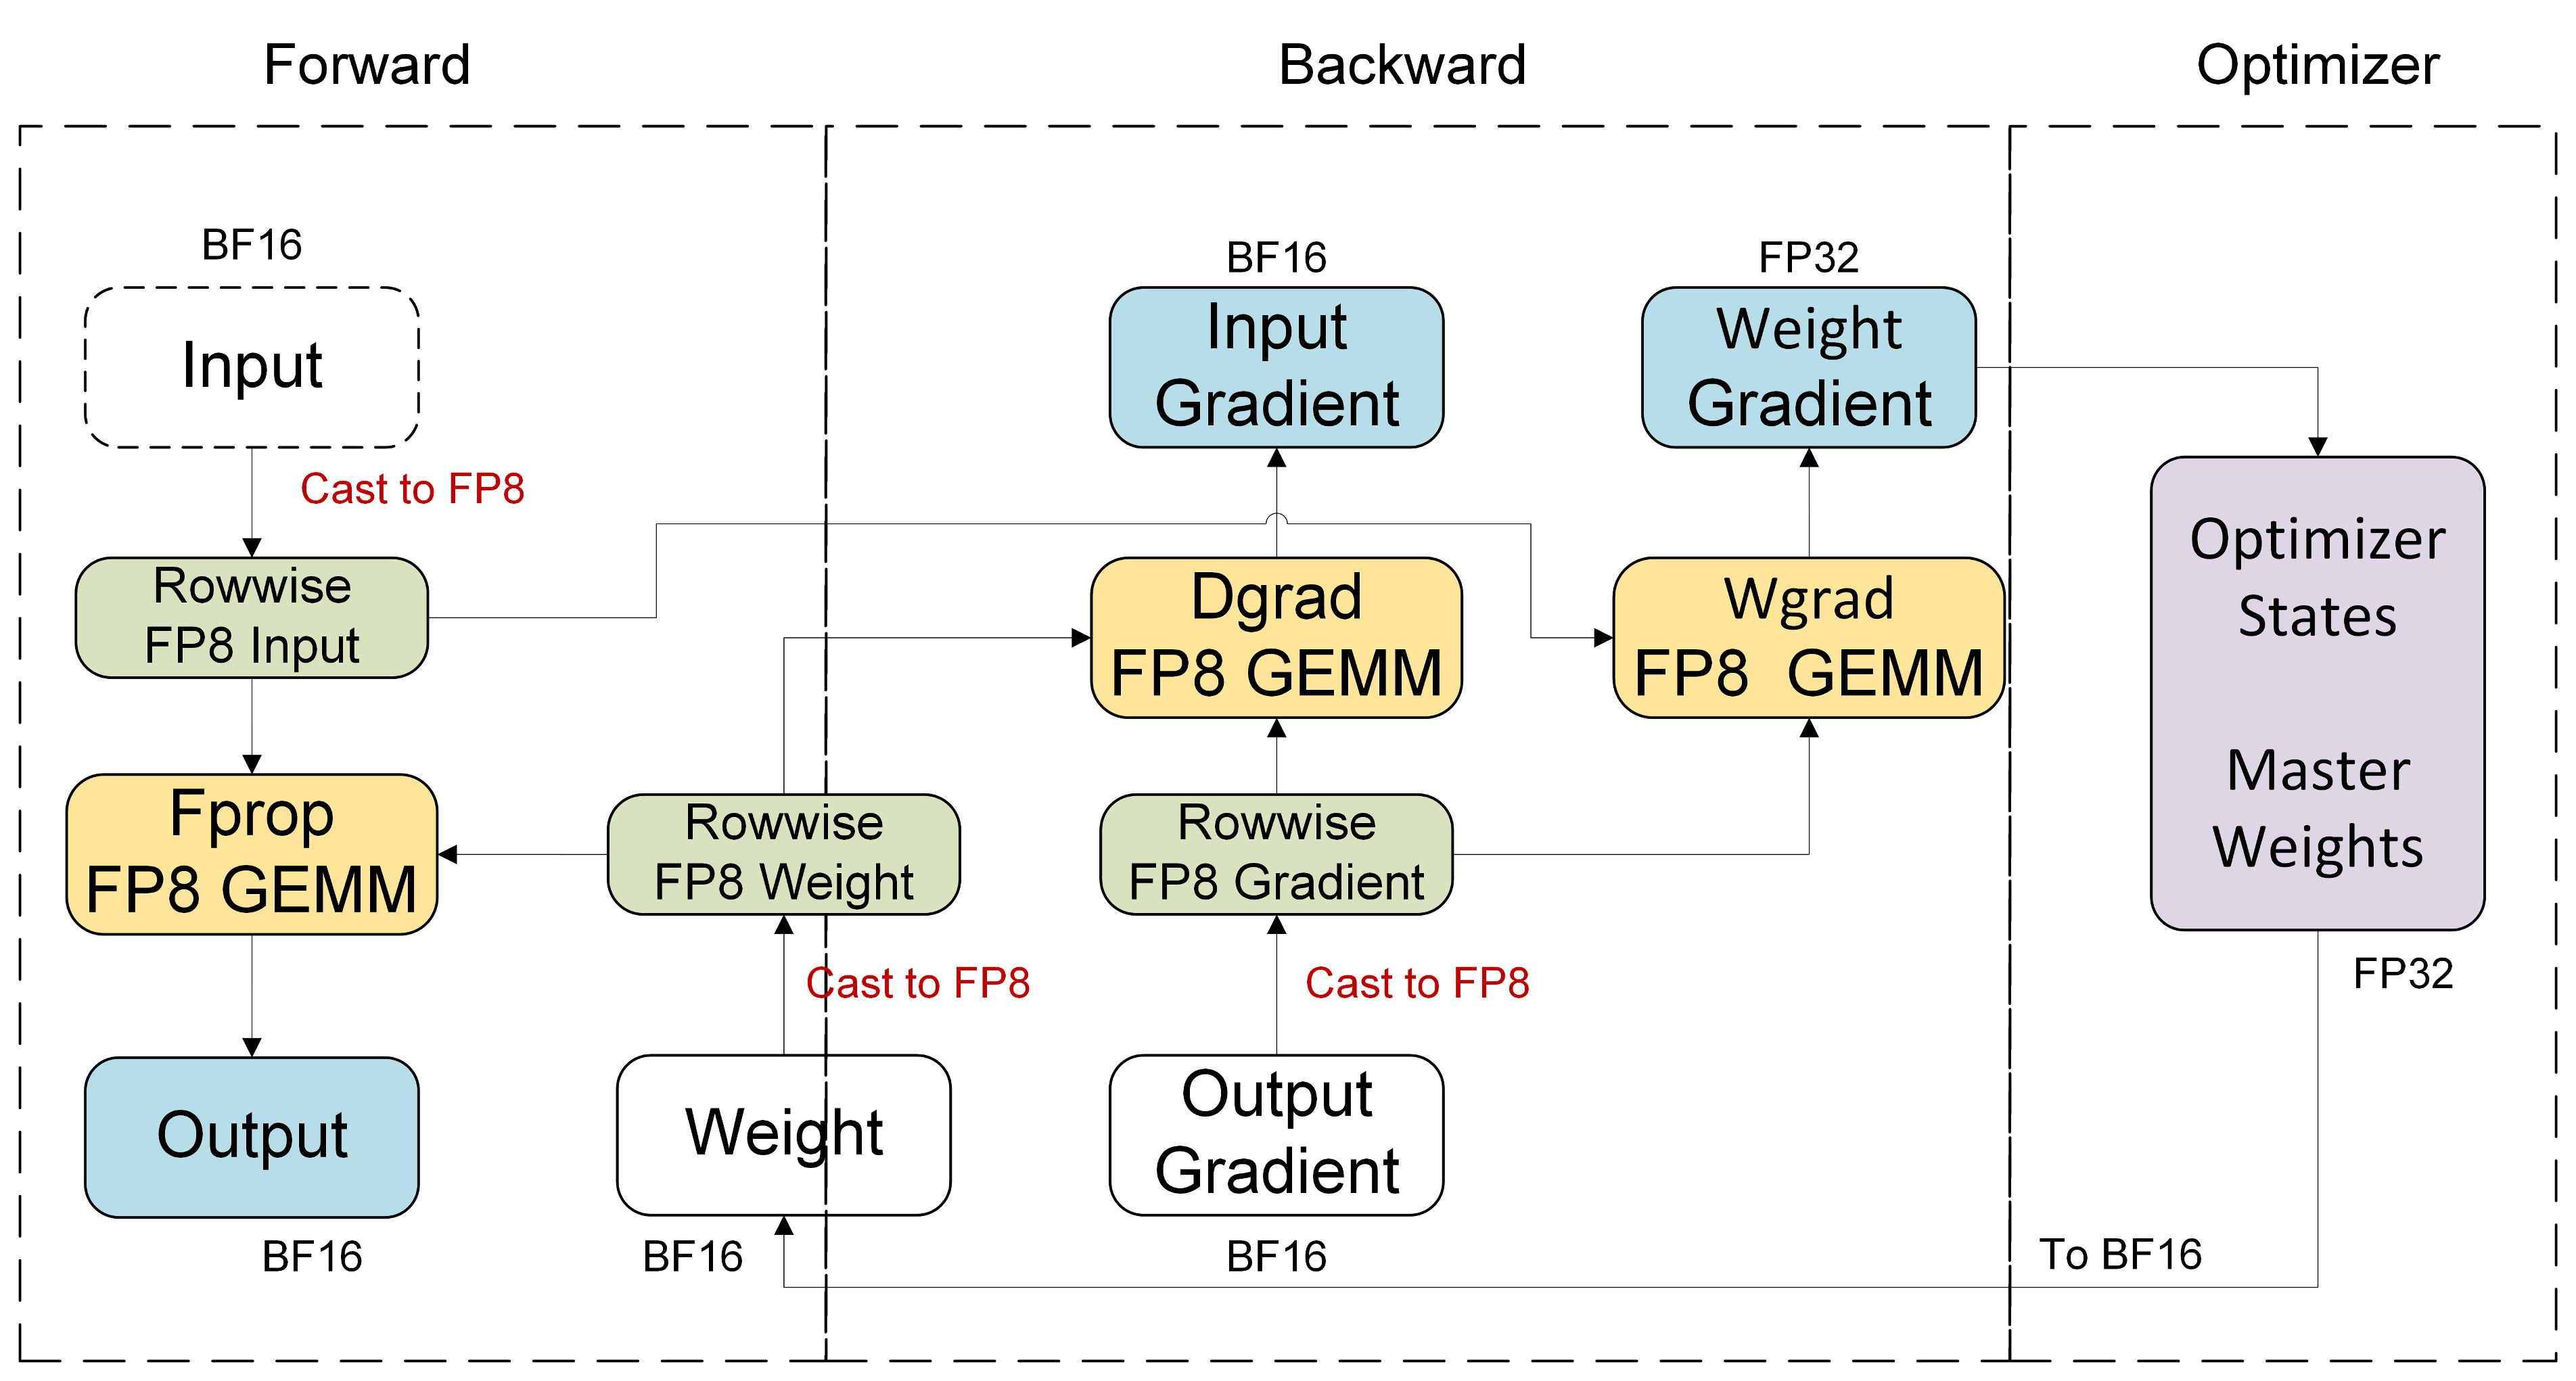
\includegraphics[width=1.0\linewidth]{figures/fp8-cs-blackwell.png}
        \caption{Blackwell 平台上的每张量电流缩放。}
        \label{fig:fp8-cs-blackwell}
    \end{subfigure}
    \begin{subfigure}[t]{0.45\textwidth}
        \centering
        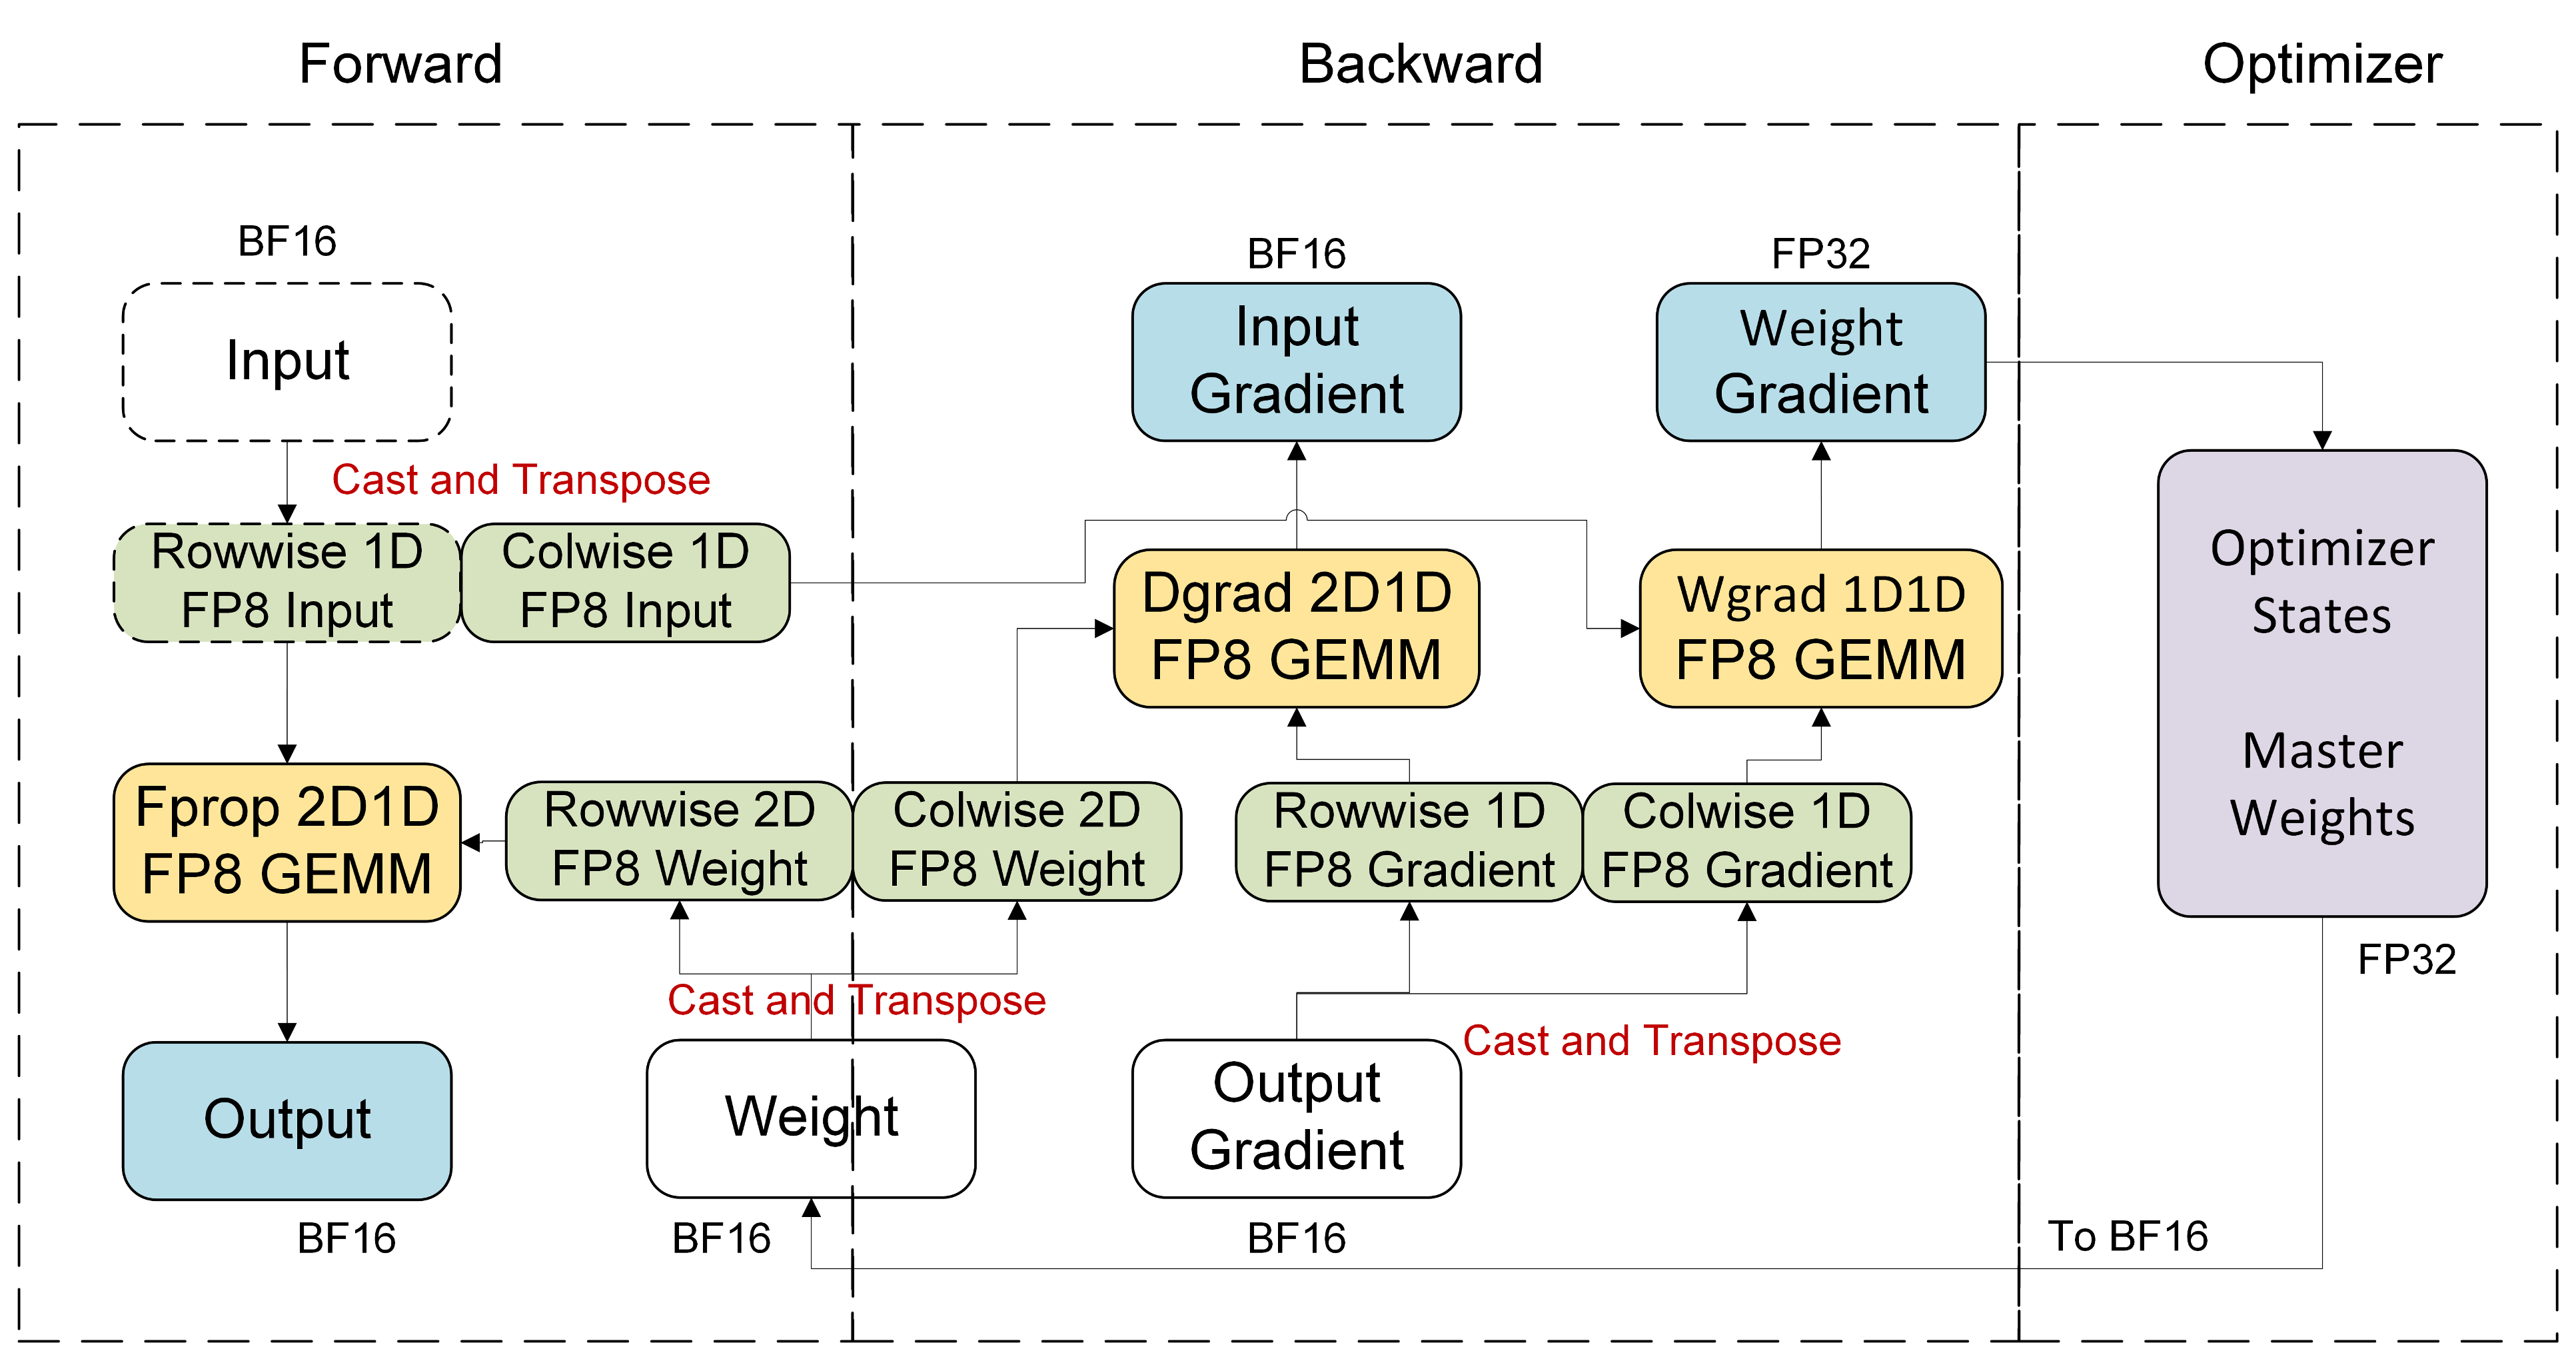
\includegraphics[width=1.0\linewidth]{figures/fp8-blockwise-hopper.png}
        \caption{Hopper 上的 Blockwise FP8 配方。}
        \label{fig:fp8-blockwise-hopper}
    \end{subfigure}
    \begin{subfigure}[t]{0.45\textwidth}
        \centering
        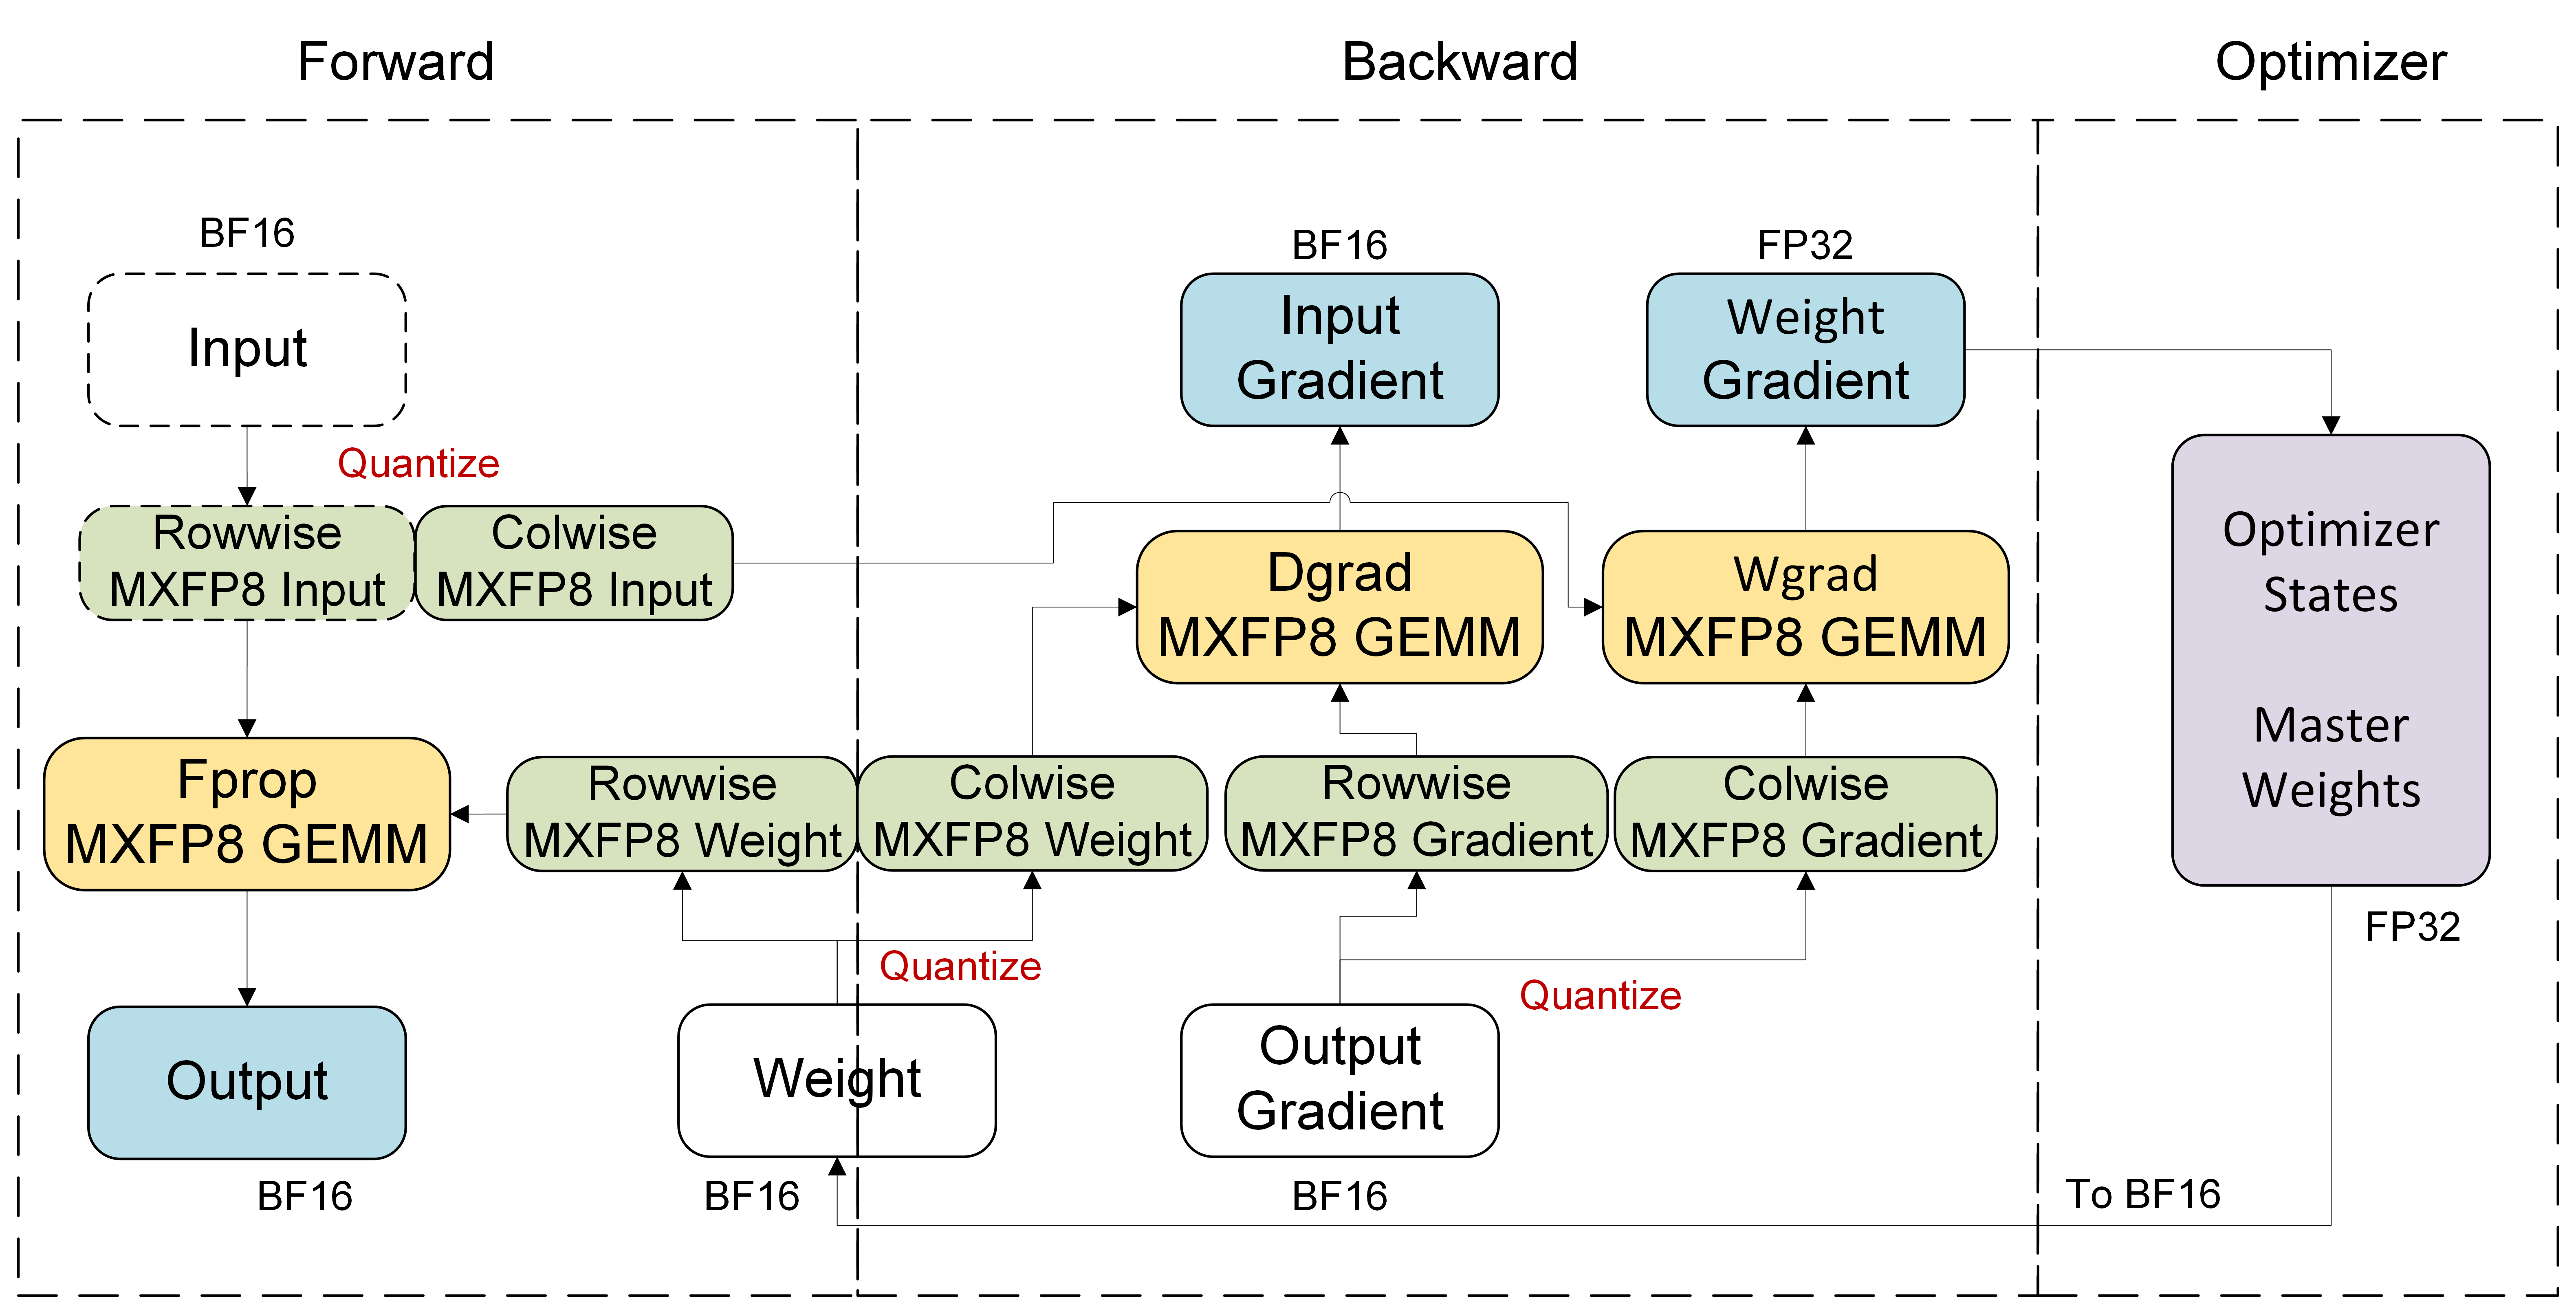
\includegraphics[width=1.0\linewidth]{figures/fp8-mxfp8.png}
        \caption{Blackwell 平台上的 MXFP8 配方。}
        \label{fig:fp8-mxfp8}
    \end{subfigure}
    \caption{使用各种 FP8 配方计算线性层。请注意跨平台量化粒度和张量布局要求的差异。}
    \label{fig:fp8-recipes}
\end{figure*}

\subsubsection{Hopper 上的 Blockwise FP8}
块式 FP8 配方对所有张量采用 E4M3 格式，量化激活和梯度 $1 \times 128$ 瓷砖和权重 $128 \times 128$ 块。块式缩放使用细粒度缩放粒度来获得更好的精度，并且已被 \textbf{已在生产中证明是成功的} 在超大规模 MoE 模型中，包括 DeepSeek-V3 \cite{deepseekai2025deepseekv3technicalreport}, 极小极大-M2 \cite{minimax_m2}、蚁灵-2.0 \cite{li2025every}等等。因此，blockwise FP8 是 Hopper 平台上推荐的 FP8 配方。

Transformer Engine 为块式配方提供高度优化的量化内核和 GEMM 内核（通过 cuBLAS），以及分层 API 和自动转换上下文，只需几行代码即可进行 FP8 训练。

\Figref{fig:fp8-blockwise-hopper} 说明了 Hopper 平台上使用分块 FP8 配方的线性层的计算，这与 Hopper 上的每张量当前缩放非常相似，除了基于图块的量化之外。

\subsubsection{布莱克威尔上的 MXFP8}
在 Blackwell 平台上，得益于原生第五代 Tensor Core 对 MXFP8 格式的支持 \cite{rouhani2023microscalingdataformatsdeep}，我们采用更细粒度的量化方案MXFP8进行训练。激活和权重都被量化为 $1 \times 32$ 粒度，E8M0用于缩放因子。理论上来说，MXFP8应该会因为更细粒度的缩放粒度而更加精确，并且由于Tensor Core对MXFP8的原生支持而具有更好的性能。因此，MXFP8是Blackwell平台上默认的FP8配方。

\Figref{fig:fp8-mxfp8} 说明了 Blackwell 平台上使用 MXFP8 配方的线性层的计算。尽管 Blackwell 支持所有布局的 FP8 GEMM，但由于另一个方向的量化，我们需要存储额外的按列量化的 FP8 数据以用于激活和权重。

MoE 训练中 MXFP8 配方的持续优化包括：
\begin{enumerate}
    \item 分组量化以减少量化开销。
    \item 将激活和量化（对于以下 GEMM）与 GEMM 内核融合。
    \item 确保 MXFP8 量化、缩放因子混合和分组 GEMM 的整个管道都是 CUDA 可绘制的。
\end{enumerate}

\subsubsection{Blackwell 上的 NVFP4}

在 \cite{nvidia2025pretraininglargelanguagemodels}中，我们提出了 NVFP4 作为 LLM 训练的 4 位微缩放格式，可提高数值保真度，同时保留 FP4 的效率优势。 

NVFP4 使用 E2M1 格式的 FP4 元素，因此通过缩放对值进行量化，因为原始 FP4 的可表示范围非常有限。一个核心设计选择是两级微尺度。 NVFP4 在 E4M3 中应用每张量 FP32 尺度和每块 8 位尺度。张量级 FP32 尺度首先将张量分布重新映射到与块缩放兼容的范围，然后块级 E4M3 尺度将每个块映射到 FP4 范围。 NVFP4 使用 16 个连续元素的块，每个块的 amax 缩放到 FP4 最大值。

在此格式设计的基础上，我们还发现稳定的 NVFP4 训练取决于量化方面的多种算法选择。特别是，我们添加了三个实用技巧：
\begin{itemize}
\item \textbf{随机 Hadamard 变换 (RHT)}：应用于权重梯度计算，减少异常值的影响。
\item \textbf{2D 缩放}：具体来说，16x16 权重块缩放（保留 FP32 张量比例）用于保持前向和后向传递之间的权重量化更加一致，并减少前向/后向量化不匹配。
\item \textbf{随机舍入}：用于梯度，以减少 FP4 转换期间的舍入偏差，因为确定性舍入会引入损害收敛的偏差。
\end{itemize}
这些添加是本文中使用的训练方法的关键部分，对于更大规模的收敛非常重要。

\begin{figure}[ht]
    \centering
    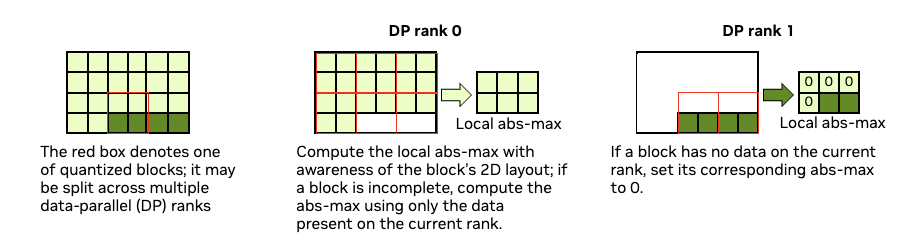
\includegraphics[width=1\linewidth]{figures/native_fp8_blockwise.png}
    \caption{用于按块缩放的 FP8 主要权重量化方案。}
    \label{fig:native_fp8_blockwise}
\end{figure}

\subsubsection{FP8/FP4 主要重量：消除冗余存储}\label{subsec:fp8-primary-weights}
传统的降低精度训练维持三层参数层次结构：用于优化器更新的 FP32 主权重、作为中间表示的 BF16 模型权重以及用于前向和后向 GEMM 计算的 FP8/FP4 权重。这通过维护 BF16 和 FP8/FP4 参数副本引入了冗余内存开销。

\textbf{本机 FP8/FP4} 通过建立从 FP32 主权重到 FP8/FP4 计算权重的直接转换路径，完全绕过 BF16 中间层，减少内存占用并加速参数 AllGather，消除了这种冗余。

实现原生 FP8/FP4 的核心挑战在于管理 FP8/FP4 张量所需的量化元数据。我们提供支持不同 FP8/FP4 配方（延迟缩放、电流缩放、块式缩放、MXFP8 和 NVFP4）的统一接口，处理 TransformerEngine 实现中特定于版本的差异，确保跨版本的兼容性。

在分布式优化器的每个优化器步骤中，FP32 参数分片都会根据减少的梯度进行更新。随后，这些更新的 FP32 分片使用适当的缩放因子直接量化为 FP8/FP4 格式。量化过程根据 FP32 值计算 amax，更新数据并行等级之间的缩放因子以保持一致性，并将量化的 FP8/FP4 值写入模型参数缓冲区。这种直接路径消除了维护 BF16 参数的内存开销，这对于参数内存可能超过数百 GB 的大型语言模型尤其有效。

更具体地说，延迟缩放和当前缩放的 FP32 分片的量化分三个步骤进行，请参阅 \figref{fig:native_fp8_current_scaling}:
\begin{itemize}
    \item 第 1 步：从主重量中获取局部最大腹肌。如果某个权重在当前rank上没有分片部分，则将其对应的abs-max设置为0。
    \item 步骤2：通过AllReduce获取全局abs-max。
    \item 第 3 步：使用全局最大腹肌和主权重进行部分投射。
\end{itemize}

\begin{figure}[ht]
    \centering
    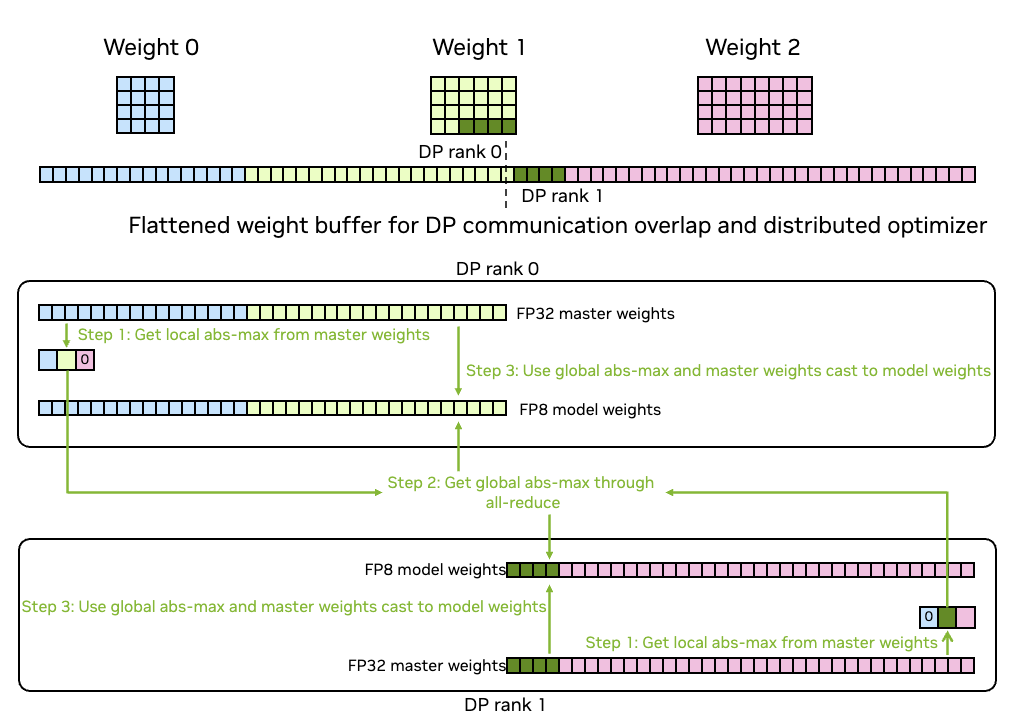
\includegraphics[width=1\linewidth]{figures/native_fp8_current_scaling.png}
    \caption{FP8 主要权重量化方案，用于延迟缩放和每张量当前缩放。}
    \label{fig:native_fp8_current_scaling}
\end{figure}

在Blockwise配方中，权重的abs-max是在2D块上计算的，因此我们不能直接使用归约内核来获得局部abs-max。我们实现了专门的内核，它了解权重的 2D 布局以及主权重和原始权重之间的对应关系，以计算ABS-MAX，请参阅 \figref{fig:native_fp8_blockwise}。

FP8/FP4初级权重的另一个优点是参数AllGather通信量大大减少（参见章节 \ref{sec:comm_wall_quantized_training}).


\subsection{MoE特有的低精度训练挑战和解决方案}

前面的小节介绍了适用于任何深度学习模型的降低精度训练的基础知识。 MoE 架构为降低精度的训练带来了独特的挑战，需要超出标准实施的专门解决方案。

\subsubsection{填充和取消填充的融合：动态形状对齐}
FP8 和 FP4 GEMM 要求张量维度与特定倍数对齐：每个张量和分块配方为 16，MXFP8 和 NVFP4 为 32。这些填充要求源自每个量化方案的块缩放粒度，以及张量内存加速器 (TMA) 访问沿 GEMM 点积维度保持 16 字节对齐的要求。在前向传递中，隐藏维度 K 是点积维度，通常已经通过模型设计进行了对齐。然而，在权重梯度GEMM中，点积维数对应于令牌维数M，其动态变化并且常常不能满足对齐要求。因此，沿着标记维度进行零填充是必要的。为了进一步启用具有较低 CPU 开销和 CUDA Graph 兼容性的分组量化内核，我们将每个专家的令牌填充增加到 128。 \ref{sec:fp4-quant-fusion} 解释了为什么 NVFP4 分组量化内核需要更大的填充；同样的原理也适用于 MXFP8 分组量化。总之，应用于令牌维度的最终填充是由路由专家层中涉及的所有内核的要求共同确定的。

我们的基线解决方案是针对不同专家的多个输入张量的融合填充和取消填充内核。然而，显式填充和取消填充内核会带来不可忽略的开销。我们提出两种解决方案：
\begin{itemize}
    \item \textbf{路由图填充}，它填充路由映射而不是接收到的令牌。这确保了每个专家的令牌数量符合要求，但代价是仅发送少量额外令牌，从而避免了昂贵的每个张量填充操作。
    \item \textbf{将填充融合到排列中} 避免全局内存读写的一次性传递，并应提供最佳性能。如果可用，它是默认选择。
\end{itemize}

% \subsubsection{FP8 EP Communications: Halving Dispatch Volume}\label{sec:fp8-dispatch-comm}
% With large EP strategies for fine-grained MoE models, EP communication becomes the primary bottleneck. To reduce this overhead, dispatch communication can be executed using FP8, halving the all-to-all volume.

% \textbf{Key insight}: Only the 1D per-token scaled recipe can make FP8 dispatch communication feasible (\figref{fig:fp8_dispatch}). In 1D per-token quantization, each token is associated with its own \textbf{row-wise} scaling factor tensor, which is preserved even after all-to-all communication. However, during weight gradient computation, the GEMM operation requires col-wise quantized (and optionally transposed) FP8 activations as input, which requires a dequantization and re-quantization (along another direction) step. To minimize potential accuracy loss due to double quantization, the E8M0 or power-of-two scale format is adopted.

% \begin{figure}[ht]
%     \centering
%     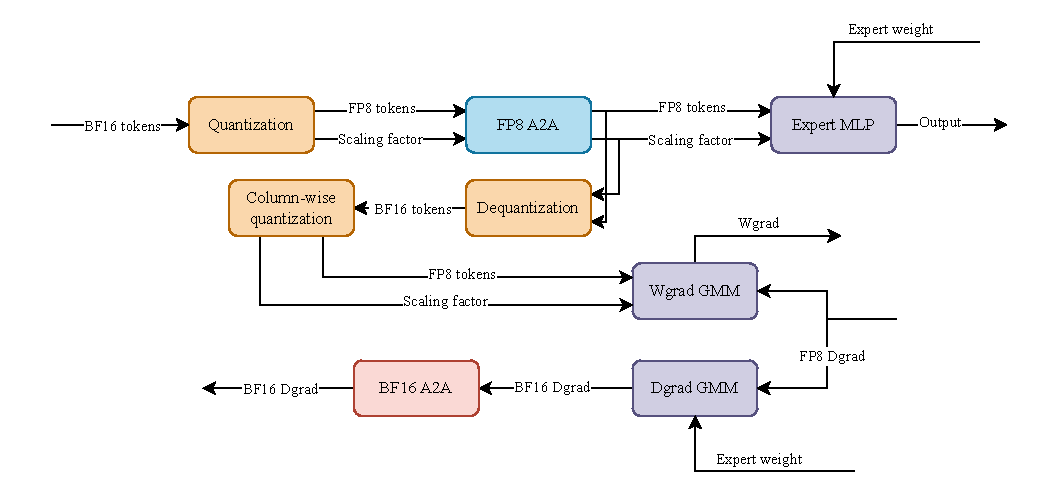
\includegraphics[width=1\linewidth]{figures/fp8_dispatch.drawio.pdf}
%     \caption{Using FP8 communication in the forward dispatch. The dequantization-quantization step is required for backward computation.}
%     \label{fig:fp8_dispatch}
% \end{figure}

% \paragraph*{Platform-Specific Implementations.}
% The blockwise recipe is used on Hopper, where FP8 GEMM only accepts inputs with a TN layout. This means the activation input must be row-major, so an additional transpose is required after column-wise quantization. In contrast, the MXFP8 recipe is employed on the Blackwell architecture, which supports arbitrary layouts and eliminates the need for this extra transpose.

% In the blockwise recipe, we need to quantize the tokens before communication. The quantized activations can directly participate in the forward computation. However, for the backward pass, we must first dequantize to reconstruct the high-precision input, then re-quantize to obtain the new result. This is because, for the same activation, the quantization dimensions used in the forward and backward phases are different. Since the Hopper Tensor Core only accepts specific layouts, a transposition step is also required beforehand.

% In the MXFP8 recipe, the process is almost identical to that of the blockwise method. Though transposition is unnecessary on the Blackwell platform, we still need the FP8 tensor quantized along different dimensions (col-wise vs. row-wise) for backward computation.

\subsubsection{分组量化和分组GEMM}

\paragraph{分组量化}

由于量化数据和缩放因子之间的填充要求不同，以及行量化和列量化引入的复杂数据布局，针对不同专家量化输入张量的一种简单方法是将量化内核逐个应用到它们。然而，它引入了大量的小内核，这增加了 CPU 开销，并且从 GPU 的角度来看效率不高。

为了解决这个问题，我们实现了分组量化内核，将多个张量的量化融合到一个内核中，这大大减少了 CPU 开销，提高了 GPU 利用率，并且是 CUDA-Graphable 的。

\paragraph{分组GEMM}
优化和 CUDA-Graphable 分组 GEMM 部分 \ref{sec:device-init}.


\subsubsection{NVFP4量化融合}\label{sec:fp4-quant-fusion}

由于我们使用数值技术来保持数值稳定性，NVFP4 量化尤其复杂，因此需要积极的内核融合来控制量化开销。在实践中，我们的 NVFP4 量化内核不仅仅是一个简单的“缩放 + 转换”内核：它需要仔细吸收训练配方逻辑，包括随机 Hadamard 变换、2D 缩放和随机舍入。 

其中，RHT 融合对延迟最敏感。如果作为单独的内核实现，Hadamard 变换将在全局内存中引入额外的全精度 (BF16) 张量读/写，从而显着增加带宽成本。通过将 RHT 与 NVFP4 量化融合，我们在单个内核中执行 Hadamard 变换和 FP4 量化，避免了额外的 BF16 流量。

第二个实施挑战是 Blackwell NVFP4 Tensor Core GEMM 是面向 TN 的，而 Wgrad 使用转置激活和梯度。因此，当 RHT 融合到 Wgrad 路径的 NVFP4 量化中时，内核还必须吸收转置，而不是依赖于单独的 BF16 转置内核（这将再次导致通过全局内存进行完整的 BF16 张量读写）。

因此，融合量化管道必须支持来自同一高精度输入的多个输出：(1) 前向 GEMM 的标准 FP4 量化，以及 (2) 后向/Wgrad 路径的转置 + RHT + FP4 量化。在训练中，我们在前向传递期间启动这个融合内核以生成两个 FP4 副本：一个由前向 GEMM 立即消耗，另一个保存用于后向。然后原始的高精度输入被丢弃，因此我们避免存储 BF16 激活，同时仍然有效地准备后向路径。

NVFP4 中的每个张量 FP32 尺度带来了进一步的复杂性。当前的 NVFP4 预训练方案，张量范围的 abs-max 是在 Hadamard 变换之后测量的，这意味着我们需要一个专用的 Hadamard+amax 内核来仅计算 amax（而不具体化变换后的 BF16 输出缓冲区）。因此，Hadamard 变换实际上被计算了两次——首先在 Hadamard-amax 内核中，然后在融合量化内核中再次计算。尽管这重复了变换计算，但它仍然比将完整变换的 BF16 张量写入全局内存更快的端到端速度，因为它避免了额外的高带宽 BF16 读/写流量。

相比之下，2D 量化在端到端吞吐量中不太明显，因为它仅适用于权重：我们可以对权重进行一次量化（例如，在第一个微批次上）并缓存量化的权重和比例，以便在以后的微批次中重用，因此其成本很大程度上被摊销。 

然而，随机舍入在关键路径上增加了内核级要求：量化内核还必须支持可选的随机舍入路径，并在内核中生成随机数（对于 dY 等梯度张量启用，否则禁用），以便 FP4 量化在单次传递中保持融合。为了保持效率，我们使用 NVIDIA cuRANDDx\cite{curanddx} 用于融合 CUDA 量化内核内的设备端随机数生成。

\paragraph{MoE 的分组 NVFP4 量化}

由于 NVFP4 配方本身的算法复杂性，支持 MoE 层的 NVFP4 量化尤其具有挑战性。在全迭代 CUDA Graph 要求下，MoE 量化路径也必须是 CUDA Graph 安全的：主机不能依赖于 CPU 上的动态专家令牌计数，而只能依赖于设备端每个专家令牌张量。这意味着输入激活不能再单独分割和量化。我们必须为完整的 NVFP4 管道实现分组量化内核。 NVFP4 输出的内存分配必须作为整个平面缓冲区进行分配，而不知道其间的形状。 

一个关键的观察结果是，大部分密集的 NVFP4 激活量化内核可以重新用于分组量化，因为不同专家的令牌在路由/排列后连续打包在内存中。主要区别在于保持性能和图形安全所需的实现限制。 

\begin{enumerate}

\item 量化线程块不应跨越多个专家的令牌，因为这会引入大量的控制流和索引开销；因此，我们将每个专家的令牌计数补零为令牌维度中线程块形状的整数倍（通常为 128）。 

\item NVFP4 转置必须针对每个专家执行（独立转置每个专家的打包激活，然后连接），这并不等同于将整个分组缓冲区转置为一个张量。 

\item NVFP4 GEMM 需要比例因子调配：比例因子必须填充为 128×4 对齐的形状，并在 GEMM 之前调配为 32×16 布局，如 cuBLAS 文档中所述\cite{cublas_sf_layout}。此缩放因子形状约束应用于每个专家 GEMM，这意味着确定所需的填充大小将隐式要求 CPU 对每个专家令牌的可见性，这不是 CUDA Graph 安全的。为了避免这种情况，我们通过构造强制每个专家 128 个令牌对齐。
\end{enumerate}

第 1) 点和第 3) 点都对每个专家施加了 128 个多个标记，这需要特定的零填充内核来满足。为了消除这种零填充开销，我们将每个专家的零填充功能融合到令牌排列内核中，因此路由的专家激活是在已经对齐和零填充的布局中生成的，并且下游分组的 NVFP4 量化/GEMM 内核可以假设所需的对齐，而无需额外的预处理。

对于 NVFP4 配方中的每张量 FP32 二级尺度，MoE 中的每张量二级尺度意味着每专家二级尺度，而不是让每个专家共享 amax 以在训练期间保持数值稳定性。这些 amax 值无法提前获知：它们必须根据路由令牌在线计算，并在每次迭代时生成为不同的每个专家 amax 值。为了有效地解决这个问题，我们利用每个专家 128 个对齐的令牌保证，并将密集输入实现调整为 CUDA-Graph 安全的分组 Hadamard-amax 内核。 

%==============================================================================
% SECTION 6: LONG-CONTEXT MOE TRAINING
%==============================================================================

\section{长情境MoE 训练}\label{sec:long-context-training}

前面的部分在假设 MoE 层主导计算成本的情况下讨论了三堵墙（内存、通信和计算效率）。这一假设适用于序列长度为 4K--8K token 的典型训练任务，其中专家计算和全民通信是主要瓶颈。然而，推理模型的兴起（OpenAI o1、DeepSeek-R1 \cite{deepseekai2025deepseekr1}等）和基于强化学习的训练创造了一个新的领域：16K、64K 甚至更长的序列。在这些长度下，MoE 训练的性能特征发生了根本性的转变：注意力在计算中占主导地位，三堵墙的相对重要性也相应发生变化。本节研究长上下文训练如何重塑 MoE 模型的三堵墙，以及Megatron Core如何应对新挑战。

\begin{figure}[ht]
    \centering
    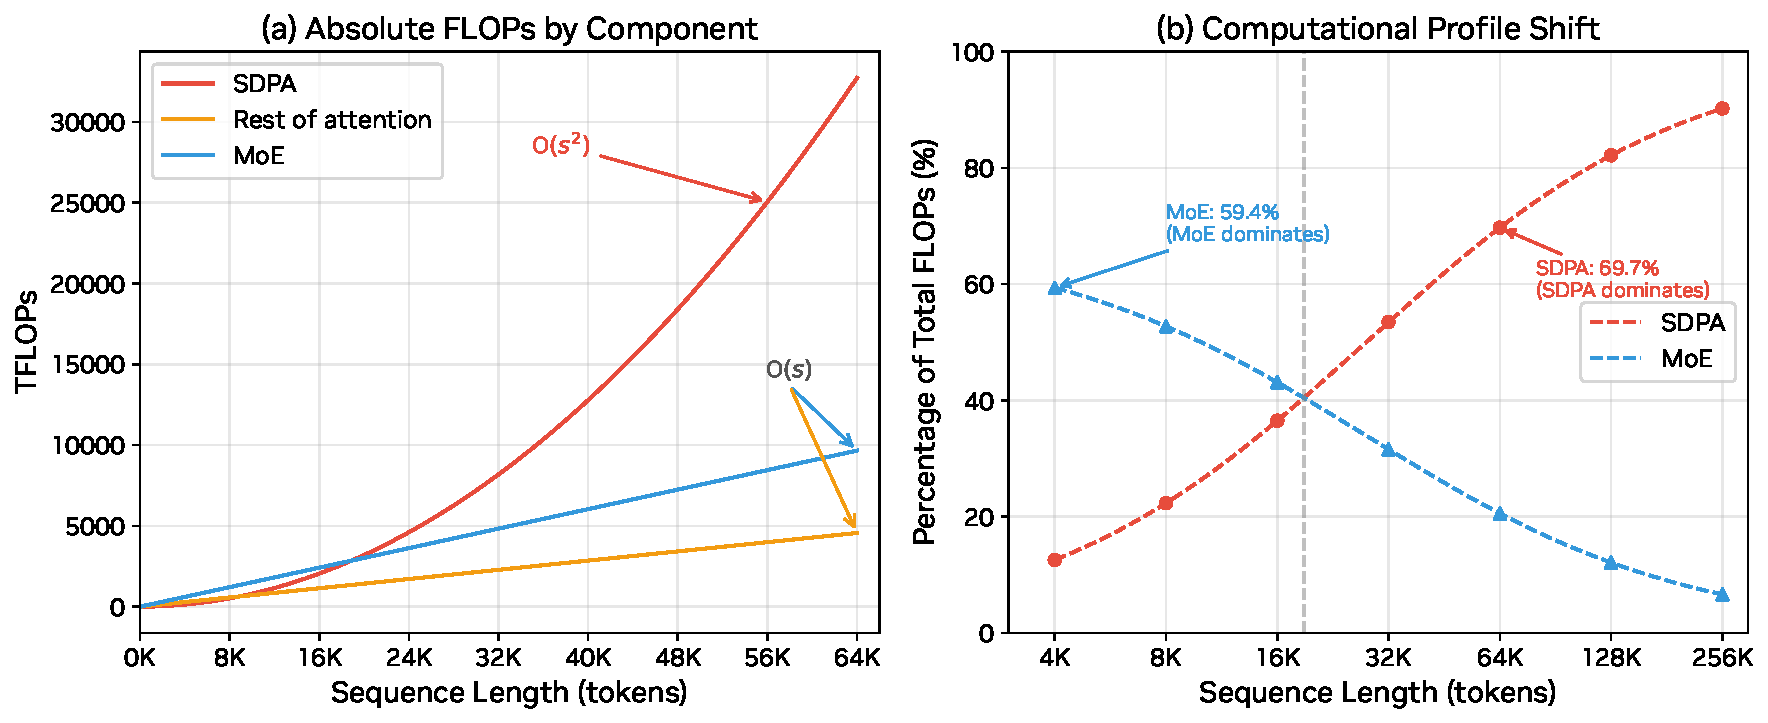
\includegraphics[width=1\linewidth]{figures/long_context_flops_ratio.pdf}
    \caption{SDPA展品 $O(s^2)$ 复杂性，而 MoE 和剩余的注意力操作表现出 $O(s)$ 复杂。因此，SDPA 在较长序列长度的计算中占主导地位。}
    \label{fig:long_context_flops_ratio}
\end{figure}

\subsection{当注意力占主导地位时：计算转变}

节中~\ref{key-features-optimizations}，我们确定 MoE 训练面临三个基本壁垒：内存、通信和计算效率。其中提出的优化（激活管理、调度程序优化、分组 GEMM 和 CUDA 图）针对 MoE 层在计算配置文件中占主导地位的场景。长情境训练从根本上改变了这一假设。关键的见解是 MoE 和注意力层之间不同的计算复杂性，如图所示 \figref{fig:long_context_flops_ratio}:
\begin{itemize}
    \item \textbf{MLP组件}：计算成本与序列长度成线性比例，表现出 $O(s)$ 复杂。
    \item \textbf{注意成分}：缩放点积注意力（SDPA）在计算成本中占主导地位，随序列长度呈二次方缩放，表现出 $O(s^2)$ 复杂。这种二次缩放激发了对有效注意力机制的广泛研究~\cite{beltagy2020longformer,zaheer2020bigbird}.
\end{itemize}

例如，对于 64K 令牌，SDPA 消耗 69\% 的 FLOP 次数，相比之下只有 10--15\% 在短序列场景中。 \textbf{注意力在计算中占据主导地位。} 幸运的是，SDPA 在大多数 GPU 加速库（例如 FlashAttention）中都进行了高度优化 \cite{dao2022flashattention,dao2023flashattention2,shah2024flashattention3} 和 cuDNN（表~\ref{tab:sdpa-cudnn-perf}），所以SDPA不会成为性能瓶颈。因此，优化重点转向内存和通信：只要我们在不引入过多开销的情况下解决这两个挑战，就可以保持训练性能。

\begin{table}[ht]
\centering
\caption{DeepSeek-V3 的 cuDNN 中的 SDPA 性能。}
\label{tab:sdpa-cudnn-perf}
\begin{tabular}{cccc}
\toprule
\textbf{平台} & \textbf{序列长度} & \textbf{转发 TFLOPS} & \textbf{向后 TFLOPS} \\
\midrule
\multirow{2}{*}{Hopper}
 & 4096  & 553  & 422 \\
 & 16384 & 638  & 523 \\
\midrule
\multirow{2}{*}{Blackwell}
 & 4096  & 1324 & 1083 \\
 & 16384 & 1698 & 1298 \\
\bottomrule
\end{tabular}
\end{table}

\subsection{管理激活内存增长}

激活记忆随序列长度的增长是长上下文训练的主要挑战。为了解决这个强化的内存墙问题，我们应用了一组协同工作的技术，这些技术由大规模 MoE 工作负载提供信息，包括 DeepSeek-V3 \cite{deepseekai2025deepseekv3technicalreport} 和Qwen3 \cite{yang2025qwen3technicalreport}。这些技术扩展了第 1 节中介绍的内存优化原则~\ref{sec:memory-wall}.

\textbf{上下文并行和张量并行。}
将上下文并行 (CP) 和张量并行 (TP) 相结合可以跨设备分配激活内存，从而实现超出 GPU 容量的序列长度。关键原则是保持子序列长度（每个 CP/TP 分片的序列长度）大致恒定，通常为 4096 或 8192。 $\text{CP} \times \text{TP}$ 序列长度使每个设备的内存保持在基线水平附近。这使得工作负载类似于短上下文训练，除了 SDPA 和 TP/CP 特定的通信之外，因此大多数短上下文优化仍然适用。

\textbf{优化器 CPU 卸载。}
在大型模型中，优化器状态通常会消耗每个 GPU 数十 GB 的字节数。 CPU 卸载几乎可以完全回收这些内存，但代价是传输和主机端优化器开销。因此，选择是内存空间和吞吐量之间的权衡。对于 256 个 H100 GPU 上的 DeepSeek-V3，约为 50\% MFU和序列长度至少16K，最坏情况开销约为2\%。尽管确切的权衡取决于模型大小、序列长度和集群规模，但优化器 CPU 卸载对于长上下文训练通常是值得的。

\textbf{选择性重新计算。}
重新计算通过丢弃向前的中间激活并向后重新生成它们来计算内存。关键是基于内存与计算权衡的模块级选择性。在长上下文设置中，SDPA 在总计算中占主导地位，因此重新计算 SDPA（Megatron-Core 中的核心注意力重新计算）通常过于昂贵。相比之下，重新计算低成本组件（例如 MLP 相关模块）通常可以提供更好的净收益。对于 64K 序列长度的 DeepSeek-V3，SDPA 贡献高达 72\% 总计算量； recomputing it adds about 18\% 计算开销，导致大约 16\% 性能损失，仅节省 9 GB 内存。相反，重新计算非 SDPA 组件可在全局范围内节省 89.8 GB，同时对性能影响相当或更低。因此，我们建议禁用核心注意力重新计算并优先考虑其他模块的重新计算。

实际上，CP 和 TP 是长上下文记忆效率的主要机制。优化器 CPU 卸载和选择性重新计算可以提供额外的空间，尤其是在内存受限的平台上。这些技术可以很好地协同工作，并且可以根据需要进行组合。

\subsection{上下文并行与张量并行}

由于CP和TP是长上下文训练中最有效的两种策略，因此实际问题是当注意力主导计算时如何将它们结合起来。

CP和TP在长情境训练中都会减少激活记忆，但它们的通信模式和记忆效果有所不同（图~\ref{fig:cp-comm-type}）。 CP 沿序列维度划分激活，并将激活内存减少为 $\text{CP}$。对于SDPA，CP有两种通信模式：点对点（P2P）和全对全（all-to-all）。 P2P CP以环形模式交换CP组内的KV缓存，与SDPA计算重叠~\cite{liu2023ringattention,brandon2023striped,jacobs2023deepspeedulysses}。 All-to-all CP 在 SDPA 之前将张量从序列分片形式转换为头分片形式，然后恢复序列分片形式。 TP 另外对线性权重进行了分片，减少了参数内存，但在线性层中引入了额外的集合。在 all-to-all CP 和 TP 中，SDPA 都在头分片张量上运行，这增加了每个分片子序列的长度并可以提高 SDPA 内核效率。

\begin{figure}[ht]
    \centering
    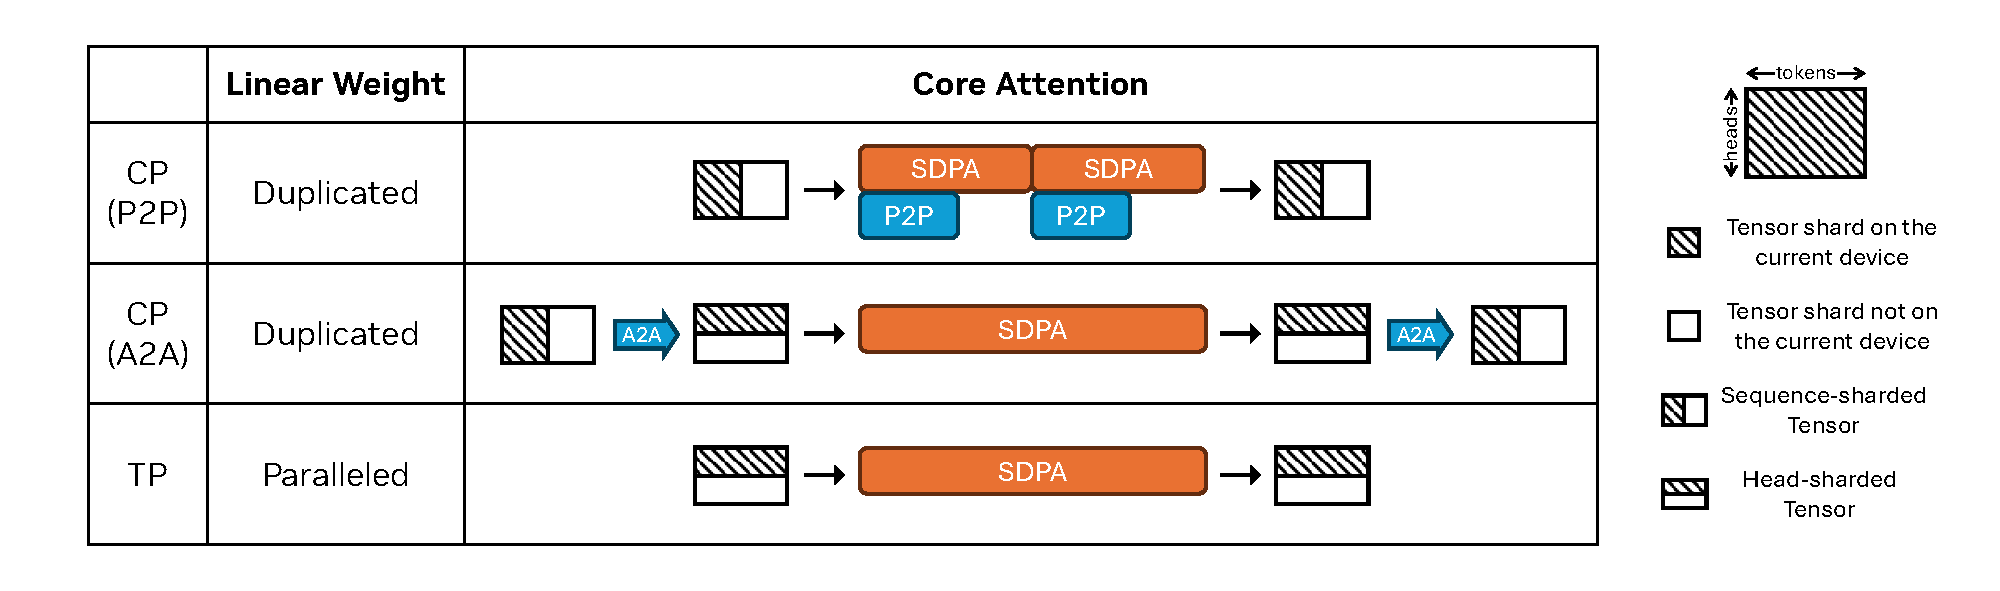
\includegraphics[width=1\linewidth]{figures/cp_comm_type.pdf}
    \caption{TP和两类CP的通信和计算模式。}
    \label{fig:cp-comm-type}
\end{figure}

在实际应用中，P2P CP是较为常见的CP模式。相对于TP，它的主要优点是通信与计算自然重叠，而TP通信往往更难隐藏。然而，TP 减少了密集的参数内存并可以提高 SDPA 效率。因此，TP 通常是节点内的首选，因为通信速度快且内存优势很强。在节点之间，P2P CP 通常变得更可取，因为 TP 通信开销会增加，而 P2P 重叠仍然有效。 All-to-all CP 介于两者之间：它避免了 P2P CP 使用的多步环交换，也避免了 TP 引入的线性权重分片开销。在实践中，当不希望进行环式交换且TP通信成本较高时，通常将All-to-all CP与TP结合起来进行节点内执行。

Megatron-Core 支持将两个 CP 后端组合为 \textbf{分层CP}，启用与 TP 的拓扑感知配对。一个实用的起点是在节点内部使用带有 TP 的all-to-all CP 来提高 SDPA 内核性能并减少参数内存，同时使用跨节点的 P2P CP 来保留通信计算重叠。这些是指导原则而不是硬性规则，但它们作为 TP/CP 调整的初始配置效果很好。

\subsection{用于可变长度训练的打包序列}\label{subsec:packed-sequence}

前面的小节研究了当序列长度增加时，三堵墙（内存、通信和计算效率）如何变化。这些分析假设每批内的序列长度固定。然而，实际训练场景，特别是强化学习和监督微调，通常涉及可变长度序列，这会带来额外的效率挑战。

传统的批处理需要将每个批次内的所有序列填充到最大长度，当序列长度变化很大时，会导致大量浪费~\cite{krell2021efficient}。例如，如果一个批次包含长度为 4K、8K 和 32K 令牌的序列，则所有序列都必须填充到 32K，从而浪费 $\sim$60\% 填充标记上的计算和内存。 This inefficiency compounds the memory and compute challenges discussed above.

为了解决这个问题，Megatron-LM 引入了 \textbf{打包序列} 在单个批次内处理可变长度序列，而不会造成填充浪费。此外，为了解决变长序列引起的DP不平衡和CP效率低下的问题，我们引入了 \textbf{动态上下文并行性（Dynamic-CP）}，它结合序列包装计划，在每个微批次的基础上自适应地选择有效的 CP 大小。

\subsubsection{打包序列支持}\label{subsec:packed_sequence_support}

Megatron-LM 支持打包序列，允许在单个批次内连接和处理多个可变长度序列，而无需序列间填充。这是通过 THD（总令牌 $\times$ 头 $\times$ Dimension）张量格式，与传统的 SBHD（序列 $\times$ 批 $\times$ 头 $\times$ 尺寸）格式。 THD 将注意力张量表示为 \texttt{[total\_tokens, num\_heads, head\_dim]}，其中来自不同样本的序列沿着标记维度串联。

核心机制依赖于累积序列长度跟踪，它标记了打包张量中每个单独序列的开始和结束位置。这些参数通过注意力机制传播到 Transformer Engine 的融合内核，从而实现尊重序列边界的高效 SDPA 和 RoPE 操作。注意力计算使用累积序列长度来确保来自不同序列的查询和键不会相互关注，从而保持正确性，同时消除填充开销。

Megatron-LM 中的实现支持跨多个训练场景的打包序列：
\begin{itemize}
    \item \textbf{强化学习}：装箱算法将可变长度的轨迹分组到固定大小的箱中，从而最大限度地提高 GPU 利用率。
    \item \textbf{多式联运培训}：具有可变图像标记计数的视觉语言模型使用打包序列来处理来自不同数量的视觉块与文本标记组合的异构序列长度。
    \item \textbf{上下文并行集成}：当上下文并行性启用并满足填充要求时，系统会自动切换到 THD 格式，并提供填充和未填充的累积长度来处理通信对齐，同时保持计算效率。
\end{itemize}

打包序列支持的好处在长上下文场景中尤其明显。对于使用思维模型进行 RL 训练，序列长度可能从数百到数万个 token 不等，打包序列可以减少 40--60 的内存使用量\% 并将训练吞吐量提高1.5--2$\times$ 与传统的基于填充的方法相比。随着上下文长度超过 32K 令牌，这种效率增益变得越来越重要，否则填充浪费将主导内存消耗并显着减少有效批量大小。

\subsubsection{打包序列的动态上下文并行性}
\label{subsec:dynamic-cp}

虽然 THD 格式的打包序列消除了填充浪费，但它们并不能消除数据并行 (DP) 等级之间的计算不平衡。即使打包样本具有相同的总标记计数，由于点积注意力相对于子序列长度的二次复杂度，它们的注意力工作负载仍然可能有很大差异。例如， \Figref{fig:packing-sequences} 显示序列打包为相等的总长度，但作为 \Figref{fig:packing-sequence-imbalance} 表明，他们的计算工作负载差异很大。

这种 DP 不平衡会导致 GPU 在梯度同步点闲置，并可能进一步放大管道并行气泡。此外，当启用上下文并行性 (CP) 时，通常会选择静态 CP 大小来满足批次中最长打包样本的内存要求。因此，适合较少设备的较短封装样本仍被迫使用相同的 CP 大小，从而导致不必要的 CP 通信。在实践中，CP通信预计会被注意力计算隐藏；然而，在由许多短子序列组成的打包序列下，每个 CP 分片的计算可能不足以隐藏 CP 集合，特别是当 CP 跨越节点间链路时。我们将这种效应称为 CP 低效率。


    \begin{figure}[ht]
      \centering
      \begin{subfigure}[b]{0.48\textwidth}
        \centering
        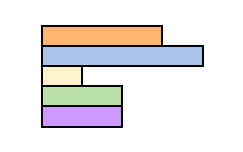
\includegraphics[width=0.8\textwidth]{figures/unpacked_sequence.pdf}
        \caption{解压序列。}
        \label{fig:unpacked-sequence}
      \end{subfigure}
      \hfill
      \begin{subfigure}[b]{0.48\textwidth}
        \centering
        \raisebox{0.8cm}{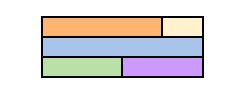
\includegraphics[width=0.8\textwidth]{figures/packed_sequence.pdf}}
        \caption{打包序列。}
        \label{fig:packed-sequence}
      \end{subfigure}
      \caption{未打包序列与打包序列。}
      \label{fig:packing-sequences}
    \end{figure}

    \begin{figure}[ht]
      \centering

        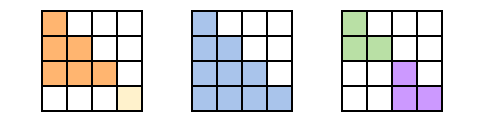
\includegraphics[width=0.8\textwidth]{figures/packed_sequence_imbalance.pdf}
        \caption{计算打包序列上因果注意力的不平衡。}
      \label{fig:packing-sequence-imbalance}
    \end{figure}

为了解决 DP 不平衡和 CP 效率低下的问题，我们引入了动态上下文并行（Dynamic-CP） \cite{nvidia_dynamiccp_blog}，它结合包装计划，在每个微批次的基础上自适应地选择有效的 CP 大小。关键的观察结果是，调整 CP 大小相对轻量级：它只改变令牌切片的划分方式以及注意力算子使用哪个 CP 通信组，而不需要任何参数重新分配或优化器状态迁移。因此，Dynamic-CP 为可变长度训练提供了一种实用的动态并行形式，并且框架开销最小。相关工作，包括ByteScale~\cite{ge2025bytescale} 和WLB-LLM~\cite{wang2025wlb}，解决类似的负载平衡挑战。


例如，考虑以下情况 \Figref{fig:input-sequences} 具有三个序列。我们假设只有两个 GPU 可用。如果我们采用标准 CP2 配置（即 DP=1，CP=2），工作负载将分两个微批次执行，如下所示 \Figref{fig:standard-cp}。在 microbatch-0 中，橙色序列足够长，必须在两个 GPU 之间进行分区。在 microbatch-1 中，打包的蓝色和绿色序列也分布在两个 GPU 上。然而，这对蓝色和绿色序列引入了不必要的分割，因为两个序列都可以适合单个 GPU 而不需要分区。

如图所示 \Figref{fig:dynamic-cp}，使用 Dynamic-CP，microbatch-0 中的橙色序列仍然需要 CP=2。在 microbatch-1 中，我们不再需要分割蓝色和绿色序列；相反，我们让它们每个都以 CP=1 独立运行。

    \begin{figure}[ht]
      \centering
      \begin{subfigure}[b]{0.19\textwidth}
        \centering
        \raisebox{0.8cm}{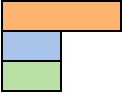
\includegraphics[width=0.8\textwidth]{figures/sequence_example.pdf}}
        \caption{输入序列。}
        \label{fig:input-sequences}
      \end{subfigure}
      \hfill
      \begin{subfigure}[b]{0.3\textwidth}
        \centering
        \makebox[\linewidth][c]{\raisebox{0.2cm}{\hspace*{-0.8cm}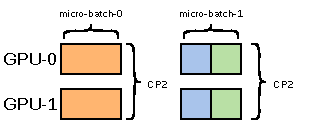
\includegraphics[width=1.4\textwidth]{figures/standard_cp.pdf}}}
        \caption{标准 CP2。}
        \label{fig:standard-cp}
      \end{subfigure}
        \hfill
      \begin{subfigure}[b]{0.3\textwidth}
        \centering
        \makebox[\linewidth][c]{\raisebox{0.2cm}{\hspace*{-0.8cm}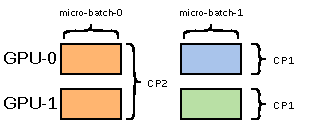
\includegraphics[width=1.4\textwidth]{figures/dynamic_cp.pdf}}}
        \caption{动态CP。}
        \label{fig:dynamic-cp}
      \end{subfigure}

      \caption{打包序列的动态上下文并行性。}
      \label{fig:dynamic-cp-example}
    \end{figure}


为了使每微批次 CP 大小调整在 Megatron-Core 中切实可行，Dynamic-CP 避免了任何昂贵的模型状态重新分配。相反，它将 CP 大小调整视为轻量级运行时选择：仅更改令牌切片的分区方式以及注意力操作符使用哪个 CP 通信组。具体来说，不是将每个等级绑定到单个静态构造的 \texttt{cp\_group}，框架在初始化期间为每个等级预先构建多个 CP 组，其中候选 \texttt{cp\_size} 范围从 1 到 \texttt{dp}$\times$\texttt{cp} （仅限于二人的权力）。在运行时，调度程序选择有效的 \texttt{cp\_size} 对于每个微批次和相应的预构建 \texttt{cp\_group}，启用动态 CP，而不会产生动态创建通信组的开销。

Dynamic-CP 专为 THD 布局而设计，其中可变长度序列在长度约束下打包，原始批次/序列维度折叠为令牌维度。一个直接的结果是微批次的数量不再是一个固定的数量 \texttt{global\_batch\_size} 和 \texttt{micro\_batch\_size};它可能会因迭代而变化，因为打包到每个微批次中的原始序列的数量不是恒定的。为了最大限度地减少对现有 Megatron-Core 管道调度程序的侵入性更改，Dynamic-CP 引入了轻量级 \texttt{data\_iterator\_wrapper} 围绕原来的 \texttt{data\_iterator}。对于每个全局批次，包装器 (i) 重新安排和打包序列以在 DP 等级之间创建平衡的工作负载，(ii) 选择有效的 \texttt{cp\_size} 对于每个微批次，以避免过度分片短包装样本，并且（iii）返回有效 \texttt{num\_microbatches} 对于当前迭代。由于通常只有排名的子集驱动 PP/VPP 下的调度决策，因此该框架广播动态调度元数据（包括 \texttt{num\_microbatches}, \texttt{max\_seqlen}， 和 \texttt{cu\_seqlens}）以确保跨管道阶段的一致执行。此外， \texttt{PackedSeqParams} 被扩展以携带所选的 \texttt{cp\_size} 和 \texttt{cp\_group};所有依赖于 CP 的组件（例如，位置嵌入和注意力）从以下位置检索 CP 配置： \texttt{PackedSeqParams} 而不是依赖全局静态 CP 变量。

给定 THD 中的可变长度序列，不同的样本贡献不同数量的有效标记。因此，损失是基于每个令牌计算的，以避免填充带来的偏差：
\begin{equation}
\mathcal{L} = \frac{\sum_{t\in \mathcal{V}} \ell_t}{|\mathcal{V}|},
\end{equation}
在哪里 $\mathcal{V}$ 表示打包表示中的有效（非填充）标记集。在规划方面，Dynamic-CP 求解器在 GPU 内存限制下共同确定打包和每微批次 CP 大小。由于注意力计算的规模大致为 $\mathcal{O}(S^2)$ 相对于子序列长度，而激活记忆规模更接近 $\mathcal{O}(S)$，很难同时平衡计算和内存。因此，Dynamic-CP 在面向工作负载和面向内存的决策之间交替：估计工作负载超过目标配额的微批次将被分配更大的容量 \texttt{cp\_size} 减少每列计算，之后内存成为主要约束，并通过选择计算量较少的样本来填充剩余容量，同时保留可行性。

最后，Dynamic-CP 的设计使运行时开销可以忽略不计。构建计划需要额外遍历全局批次以探测轻量级形状和序列长度元数据；通过在集群中分布探最后，Dynamic-CP 的设计使运行时开销可以忽略不计。构建计划需要额外遍历全局批次以探测轻量级形状和序列长度元数据；通过在集群中分布探测并仅收集紧凑的元数据，可以减轻 I/O 压力。求解器本身异步运行（例如，在 \texttt{data\_sampler}）与训练迭代重叠。为了保持搜索空间的可管理性，穷举搜索被微批次计数上的一维网格搜索所取代，并受到约束，以便所有 DP 排名使用相同的 \texttt{num\_microbatches}。该计数是从 \texttt{PP}$\times$1 的小倍数 \texttt{PP}，捕获每微批次工作负载和管道气泡之间的权衡；在实践中，通过选择工作负载与微批次曲线上的“拐点”并仅探索其邻域，可以进一步缩小搜索范围。


总体而言，Dynamic-CP 通过以下方式补充打包序列训练：(i) 减少由 DP 不平衡引起的同步停顿；(ii) 防止无法从大 CP 大小中受益的微批次进行不必要的 CP 通信，从而提高长上下文可变长度训练的吞吐量。根据基准测试，Dynamic-CP 产生 35--60\% 在序列长度分布高度不平衡的现实场景（例如多模态训练）中实现端到端性能改进。 \footnote{探索 \href{https://github.com/NVIDIA/Megatron-LM/pull/2000}{公关\#2000} 和 \href{https://github.com/NVIDIA/Megatron-LM/pull/2959}{公关\#2959} 使用 Megatron-Core 优化开始训练具有可变长度序列的模型。}

\subsection{概括}

长上下文 MoE 训练代表了一种独特的优化机制，其中第 ~ 节的基本假设\ref{key-features-optimizations} 必须重新审视。虽然三堵墙（内存、通信和计算效率）仍然是基本障碍，但它们的相对重要性随着序列长度的增加而发生显着变化：

\begin{itemize}
    \item \textbf{计算转变}: 注意啦 $O(s^2)$ 复杂性取代 MoE 层成为主要的计算瓶颈，消耗 $>$ 69\% 失败次数 $>$ 64K 令牌。 MoE重点优化的Section~\ref{sec:compute-wall} 仍然有价值，但不再解决主要瓶颈。
    
    \item \textbf{内存墙强化}：激活内存随序列长度变化，需要第 4 节中的并行策略~\ref{parallelism-strategies} （特别是CP和TP）结合Section~的记忆技巧\ref{sec:memory-wall} （重新计算、卸载）以维持可行的内存占用。
    
    \item \textbf{通信权衡}：CP 和 TP 之间的选择涉及通信开销、内存节省和 SDPA 计算效率之间的微妙权衡，这种平衡不同于第 3 节以 MoE 为中心的全面优化重点\ref{sec:comm-wall}.
\end{itemize}

通过结合上下文并行性、张量并行性、选择性重新计算和优化器卸载，Megatron-Core 可实现跨不同序列长度的高效训练。我们在 256 个 Hopper GPU 上以 256K 序列长度进行的实验证明了这一点：DeepSeek-V3 达到了 88\% 使用 TP、优化器 CPU 卸载和选择性重新计算的短上下文 MFU，而 Qwen3-235B-A22B 达到 129\% 其短上下文 MFU 具有 TP、CP 和选择性重新计算（后者超过 100\% 因为 SDPA 内核在主导较长序列的计算时效率很高）。打包序列和 Dynamic-CP 功能进一步将这些功能扩展到 RL 和 SFT 训练中的可变长度工作负载。


%==============================================================================
% SECTION 7: PRODUCTION Features
%==============================================================================

\section{生产特点}\label{sec:production-features}

前面的部分重点介绍了解决“三堵墙”问题的性能优化。然而，生产MoE 训练还需要稳健性、灵活性和易用性。本节介绍满足这些操作要求的功能：确保稳定训练的负载平衡、共享和潜在的专家架构、用于灵活部署的分布式检查点、升级以使用现有的密集模型，以及与多令牌预测等高级训练范例的集成。

\subsection{负载均衡和令牌丢弃}

MoE 模型中的动态路由可能会导致严重的工作负载不平衡，某些专家会比其他专家获得更多的令牌。这会导致计算效率低下、内存瓶颈和硬件利用率下降。我们通过两种协调机制来应对这些挑战：负载平衡和令牌丢弃。

\textbf{负载平衡。}
\Figref{fig:load-balancing-strategies} 说明了Megatron Core MoE 中可用的负载平衡策略。 
我们提供多种策略来鼓励统一的令牌分配。主要方法采用 \textbf{辅助损失}~\cite{lepikhin2020gshard,fedus2022switchtransformersscalingtrillion}，一个可微的惩罚项，不鼓励将所有令牌路由到一小部分专家。我们也支持 \textbf{专家选择路由}~\cite{zhou2022mixtureofexpertsexpertchoicerouting}，它将平衡路由制定为最优传输问题，并且 \textbf{辅助无损耗平衡} 通过可学习的专家偏差术语~\cite{wang2024auxiliarylossfreeloadbalancingstrategy} 根据历史负载动态调整路由决策。

\textbf{令牌掉落。}
我们支持两种具有不同容量管理策略的调度策略。在 \textit{无滴模式} （默认），所有路由令牌的处理都没有容量限制，从而以每个专家工作负载的可变性为代价最大化模型表达能力。在 \textit{可放置模式}，执行明确的专家容量限制~\cite{lepikhin2020gshard,fedus2022switchtransformersscalingtrillion}：当分配给专家的令牌超出其容量时，多余的令牌将被丢弃并通过剩余连接绕过。这提供了可预测的内存范围，在路由器初始化不良时的早期训练期间非常有用。

\textbf{静态形状的 Pad-to-Max。}
可放置模式还可以 \textit{填充到最大} 功能，它将所有专家输入填充到相同的容量限制。这将 MoE 固有的动态每个专家令牌计数转换为静态形状，从而实现诸如 CUDA 图形之类的优化（第 ~\ref{sec:cuda-graphs}）需要在迭代中固定张量维度。

\begin{figure}[ht]
    \centering
    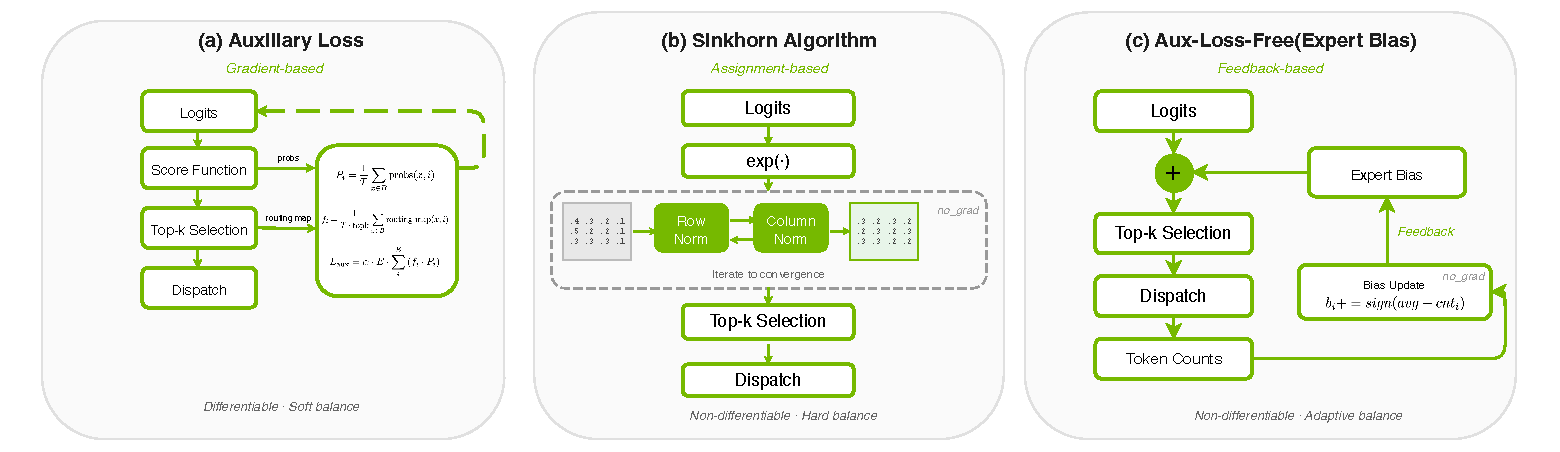
\includegraphics[width=\textwidth]{figures/load-balancing-strategies.drawio.pdf}
    \caption{Megatron-Core MoE 中的负载平衡策略。}
    \label{fig:load-balancing-strategies}
\end{figure}%

\subsection{共享专家}

一些 MoE 架构（DeepSeek-V2/V3 \cite{deepseekai2024deepseekv2strongeconomicalefficient,deepseekai2025deepseekv3technicalreport}, 琪文 \cite{qwen2025qwen25technicalreport}）包括一个共享专家，无论路由如何，都可以处理所有令牌，从而为所有令牌提供一致的基线容量（\figref{fig:shared-expert-architecture}）。当启用重叠时（\texttt{-{}-moe-shared-expert-overlap}），共享专家计算与所有通信和路由专家计算并行运行，将其延迟隐藏在调度-计算-组合管道后面。

\begin{figure}[ht]
    \centering
    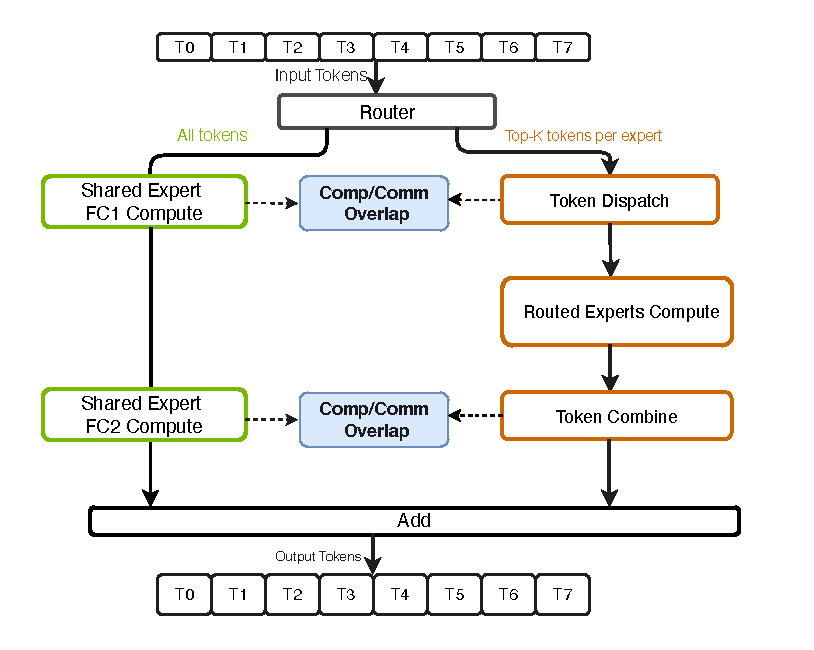
\includegraphics[width=0.7\textwidth]{figures/shared-expert-architecture.drawio.pdf}
    \caption{Megatron-Core MoE 中的共享专家架构。共享专家流程 \emph{全部} 令牌，而路由专家仅处理分配给他们的令牌。启用重叠后，共享专家计算与令牌调度/组合通信并行运行，隐藏其延迟。}
    \label{fig:shared-expert-architecture}
\end{figure}

\subsection{潜在的MoE}\label{sec:latent-moe}

在标准 MoE 中，all2all 通信在完全隐藏维度上调度令牌 \(d\)，每个专家都由权重矩阵参数化 \(\mathbb{R}^{m \times d}\) 和 \(\mathbb{R}^{d \times m}\)。潜伏MoE~\cite{elango2026latentmoe} 通过插入共享下投影来降低这两种成本 \(W_\downarrow \in \mathbb{R}^{\ell \times d}\) 在调度和向上投影之前 \(W_\uparrow \in \mathbb{R}^{d \times \ell}\) 合并后，其中 \(\ell < d\) 是潜在维度。路由仍然在完全隐藏的维度上运行，以保持路由质量；每个被路由的专家完全在压缩的潜在空间中运行；共享专家仍处于维度 \(d\)。层输出变为：
\[
\text{output}(\mathbf{x}) = W_\uparrow \cdot \Bigl(\sum_{i \in \mathcal{T}_{K,E}} p_i \, E_i(W_\downarrow \cdot \mathbf{x};\, \ell)\Bigr) + \sum_{j} E_j^{\text{shared}}(\mathbf{x};\, d).
\]

压缩比 \(\alpha = d / \ell\) 将 all2all 通信量减少一倍 \(\alpha\) （令牌在维度上发送 \(\ell\) 而不是 \(d\)）和每个专家的权重大小相同的因子（专家矩阵从 \(\mathbb{R}^{m \times d}\) 到 \(\mathbb{R}^{m \times \ell}\)）。埃兰戈等人~\cite{elango2026latentmoe} 定义两种利用这些节省的方法。在 \(\ell\text{-MoE}_{\text{eff}}\), 专家总数 \(E\) 缩放比例为 \(\alpha\) 而顶部-\(K\) 不变，以降低的推理成本保持基线精度。在 \(\ell\text{-MoE}_{\text{acc}}\) （推荐），两者 \(E\) 和顶部-\(K\) 缩放比例为 \(\alpha\)，它将推理成本恢复到标准 MoE 水平，但呈指数级扩展专家选择的组合空间（\(\binom{\alpha E}{\alpha K} \geq \binom{E}{K}^{\alpha}\)），以等成本产生更高的精度。在高达 95B 参数的范围内， \(\ell\text{-MoE}_{\text{acc}}\) 在每 FLOP 和每个参数的准确性方面始终优于标准 MoE。该架构已被 NVIDIA 的 Nemotron-3 Super 和 Ultra 型号采用。

\textbf{执行。}
LatentMoE 通过启用 \texttt{-{}-moe-latent-size}，其中设置 \(\ell\)。这 \texttt{MoELayer} 实例化两个 \texttt{TELinear} 预测： \texttt{fc1\_latent\_proj} （下投影在 \texttt{preprocess} 步骤，在路由之后但在分派之前）和 \texttt{fc2\_latent\_proj} （上投影在 \texttt{postprocess} 步骤，合并后）。专家后端（\texttt{TEGroupedMLP}, \texttt{SequentialMLP}）自动调整它们的输入和输出尺寸 \(\ell\).

\subsection{分布式检查点}

传统的检查点将保存的模型状态与特定的并行性配置紧密耦合，在更改 TP、EP、PP 或其他并行性设置时需要复杂的离线转换。我们的分布式检查点库通过以下方式解决了这个问题 \textbf{与并行性无关的检查点} 自动重新分片。

核心抽象是 \texttt{ShardedTensor} 描述符，对每个局部张量的全局形状、偏移量和分片模式进行编码。在保存期间，每个等级独立写入其本地分片（完全并行保存），消除协调器瓶颈。在加载过程中，每个等级根据以下情况确定它需要全局张量的哪些部分： \textit{新的} 分片规范并仅读取这些切片。

这使得任意并行重新配置成为可能：保存的检查点 $\text{TP}=2$, $\text{EP}=4$ 可以装载 $\text{TP}=4$, $\text{EP}=8$ 无需离线转换。该库支持 Zarr（默认）和 PyTorch Distributed~\cite{zhao2023pytorchfsdp} 存储后端。

\subsection{灵活的非对称虚拟管道并行性}\label{sec:flexible-vpp}

交错管道并行~\cite{narayanan2021efficient} 将每个物理管道阶段划分为多个虚拟阶段，并进行交错调度，从而减少管道泡沫。传统的VPP需要均匀的层分布（例如，具有 $\text{PP}=4$, $\text{VPP}=2$ 将层分布为 $[6, 6, 6, 6]$）。然而，MoE 模型表现出巨大的工作负载异质性：MoE 层、密集层、嵌入、丢失和 MTP 等专用层具有显着不同的计算成本。

我们介绍 \textbf{灵活的非对称VPP}，它允许每个虚拟阶段有不同数量和类型的层。考虑具有 61 个解码器层和 1 个 MTP 层的 DeepSeek-V3，位于 $\text{PP}=16$, $\text{VPP}=2$ （表~\ref{tab:flexible-vpp-example}）。初始等级将轻量级嵌入与 3 个密集解码器相结合（与 2 个 MoE 层的成本相匹配）。大多数等级每级拥有 2 个 MoE 解码器。最终排名战略性地放置了重MTP层和轻量损失层以平衡工作负载。

这种方法使 VPP 能够用于具有任意层数的模型，通过考虑每层计算成本来实现真正的负载平衡，并为专用层提供灵活的放置。

\begin{table}[ht]
\centering
\caption{具有灵活的非对称 VPP 的 DeepSeek-V3 的层分布（$\text{PP}=16$, $\text{VPP}=2$).}
\label{tab:flexible-vpp-example}
\begin{tabular}{lll}
\toprule
\textbf{PP等级} & \textbf{VPP 排名 0} & \textbf{VPP 排名 1} \\
\midrule
0       & 嵌入+3$\times$ 解码器 & 2$\times$ 解码器 \\
1--13   & 2$\times$ 解码器             & 2$\times$ 解码器 \\
14      & 2$\times$ 解码器             & MTP \\
15      & 2$\times$ 解码器             & 损失 \\
\bottomrule
\end{tabular}
\end{table}

这种灵活的不对称方法（\figref{fig:flexible-vpp-layout}）具有几个关键优势：（1）它为具有任意层数和组合的模型启用 VPP，消除了对模型架构设计的人为限制； （2）它通过允许对层分布进行细粒度控制来实现真正的计算负载平衡，考虑到层类型之间计算成本的巨大差异； (3)它为专用层（MTP、编码器-解码器结构等）提供灵活的放置策略，使不同的模型架构能够充分利用管道并行性的延迟隐藏优势。从业者可以设计布局，将计算量大的层分布到各个队列中，以避免内存压力并最大限度地减少管道气泡。

\begin{figure}[ht]
    \centering
    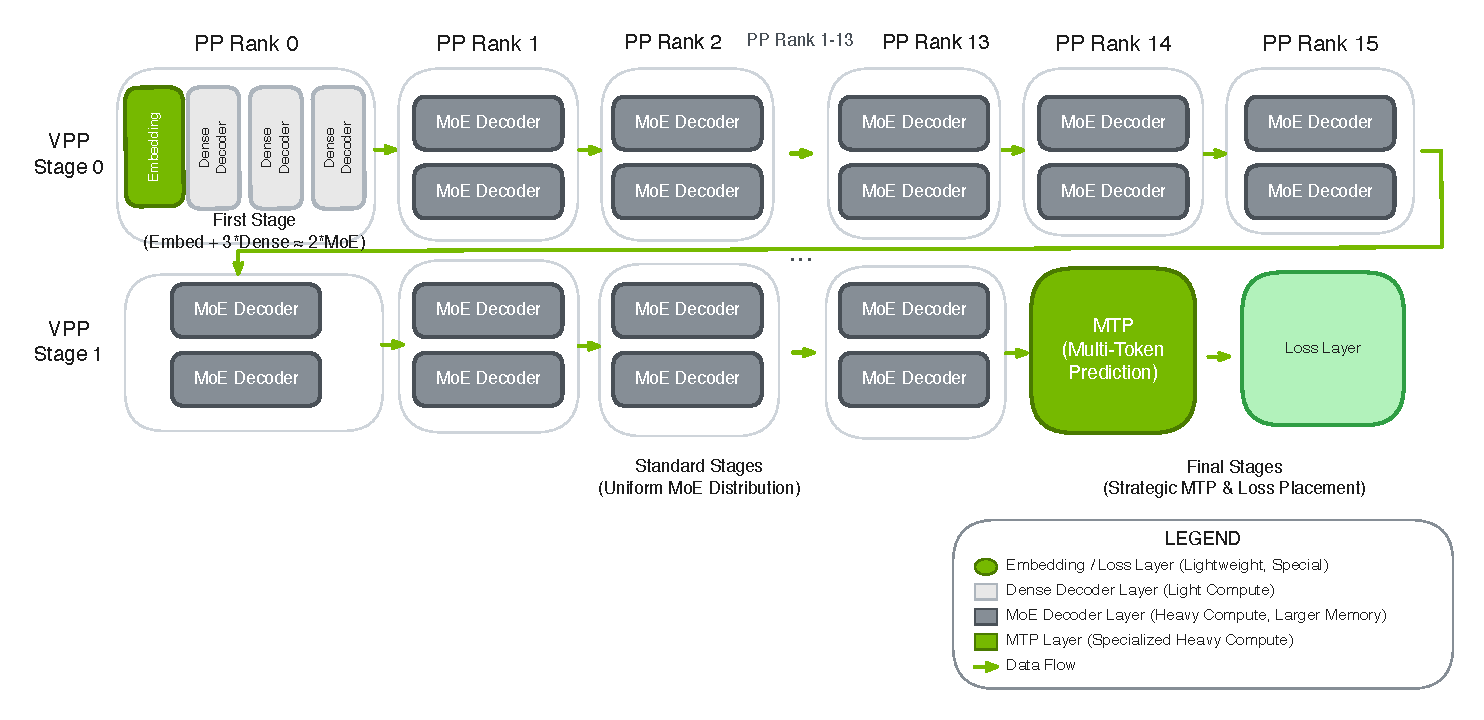
\includegraphics[width=0.95\textwidth]{figures/plots/flexible_vpp_layout_draft.pdf}
    \caption{\textbf{灵活的管道平行布置。}}
    \label{fig:flexible-vpp-layout}
\end{figure}

\subsection{升级再造}
Upcycling 将预训练的稠密模型转换为稀疏 MoE 架构，在无需从头开始重新训练的前提下扩展模型容量~\cite{komatsuzaki2022sparse,he2024upcyclinglargelanguagemodels,vavre2024llama}。我们支持虚拟组初始化和专家权重缩放，以实现将稠密检查点无缝适配到细粒度 MoE 模型。该方法采用 softmax-then-topK 路由，通过让令牌仅经过被选中的专家子集来提升表达能力，同时保持恒定或更低的推理成本，如 \figref{fig:granular_upcycling_diagram} 所示。

\begin{figure}[!ht]
    \centering
    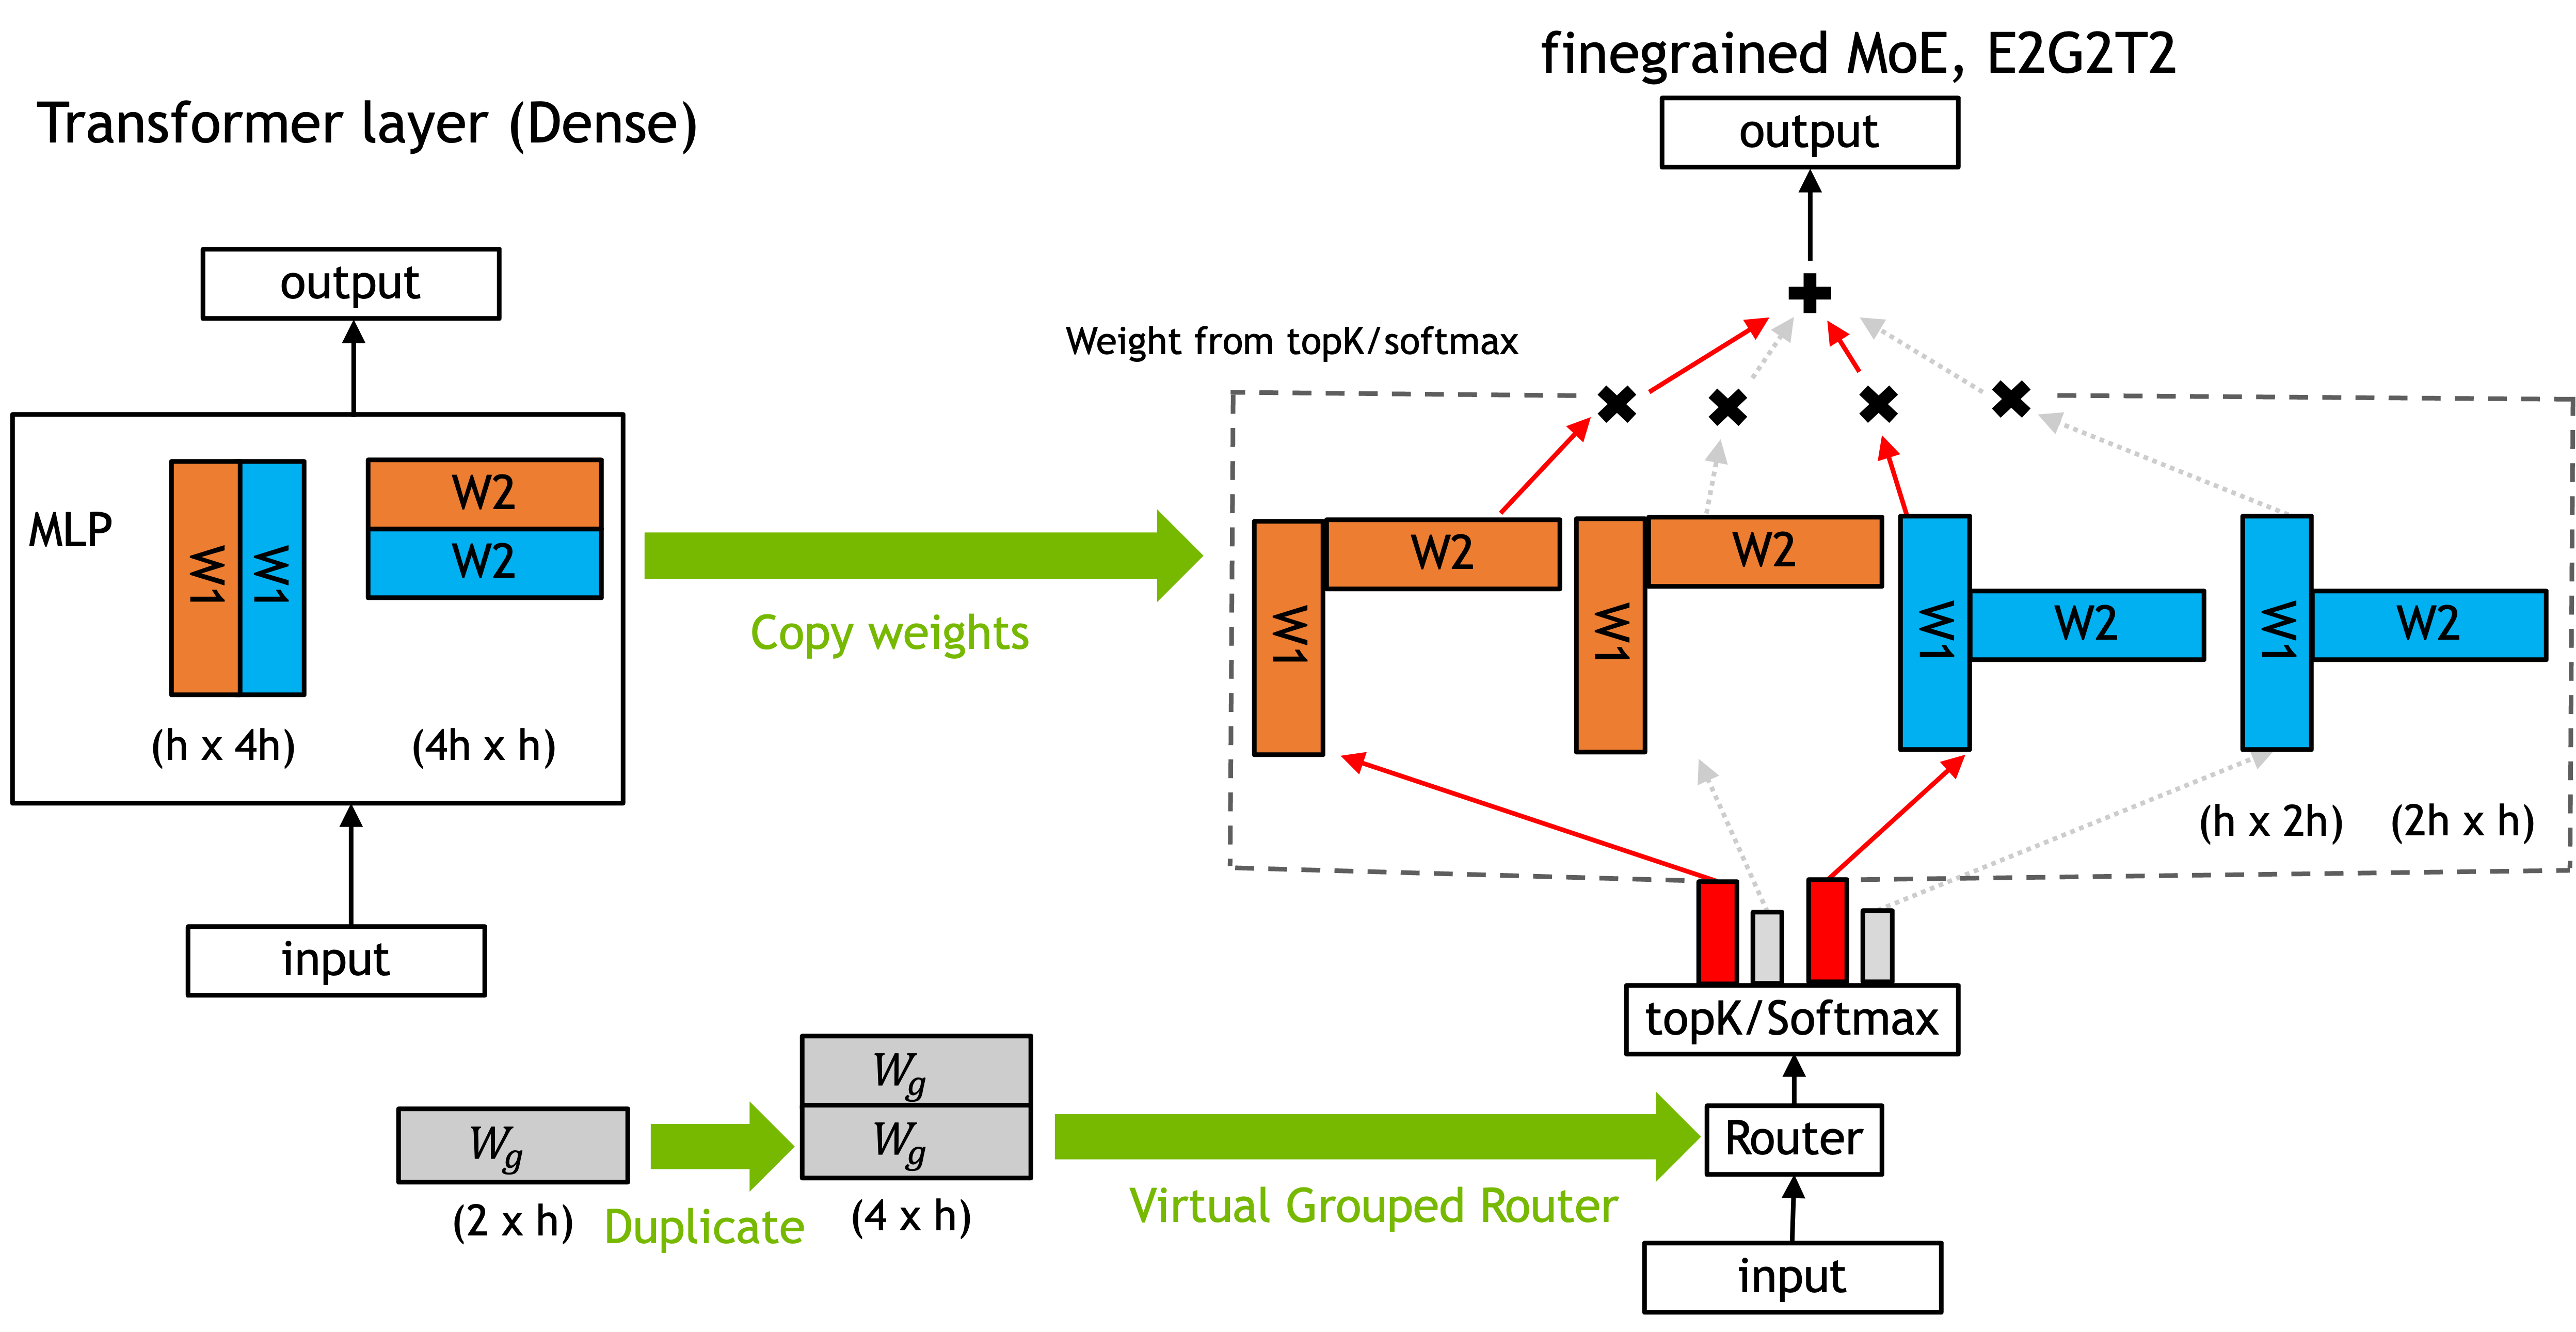
\includegraphics[width=1\textwidth]{figures/granular_upcycling.png}
    \caption{将稠密层升级再造成 E2G2T2 细粒度 MoE 的示例。E2G2T2 表示 4 个专家、top-2 路由，以及减半的中间维度大小。(1) 我们在中间维度上对 MLP 权重进行分片（$4h \rightarrow 2h$），然后复制这些分片。(2) 我们初始化一半的路由器权重，再将其复制。这保证了 Top2 总会选择每种 MLP 分片中的一个，因此在训练开始时，MoE 的输出与原始稠密模型一致。}
    \label{fig:granular_upcycling_diagram}
\end{figure}

\subsection{多令牌预测}
多令牌预测（MTP）优化模型，在每个位置预测多个连续的未来令牌，为训练提供更密集的监督信号~\cite{gloeckle2024better,deepseekai2025deepseekv3technicalreport}。与并行独立预测不同，MTP 通过隐藏状态转换维持预测之间的因果依赖性，从而加速收敛并提高生成质量。在推理过程中，模型恢复为标准单令牌预测以实现部署兼容性。

我们将 MTP 与灵活的管道并行性相集成，允许 MTP 层战略性地放置在 VPP 布局中，以实现平衡的工作负载分配。

\subsection{Muon 优化器}
与 AdamW 等执行逐元素更新的传统优化器不同，Muon 优化器通过正交化整个权重矩阵引入了矩阵感知方法~\cite{liu2025muonscalablellmtraining}。与 AdamW 相比，这改进了优化轨迹的调节并显着减少了训练步骤。

我们的集成为大规模分布式训练提供了生产就绪的支持，具有以下几个关键优势：（1）完全支持分割查询键值（QKV）权重布局，即使在注意力投影矩阵存储为单独的张量时也能实现高效的正交化； (2) 与分布式优化器无缝集成，允许优化器状态跨数据并行级别进行分片，同时保持正确的正交化语义； (3) 当 GPU 内存受限时，Muon 正交化缓冲区的 CPU 卸载。

\textbf{MuonClip。}
训练万亿参数模型带来了稳定性挑战，其中查询键点积可以无限增长，导致注意力爆炸 \cite{kimik2}。 MuonClip 通过 cuDNN、cudnn-frontend 和 Transformer Engine 中的硬件加速实现解决了这个问题。

\section{绩效评估}\label{performance-evaluations}
前面的部分描述了 Megatron-Core MoE 的架构、并行策略和优化。本节通过实证评估验证了这些贡献，展示了 Megatron-Core MoE 堆栈在不同模型配置和硬件平台上的性能。

\begin{notebox}
\textbf{生活文档。} 本节中的性能结果代表基于 Megatron-Core 的时间点快照 \textbf{v0.16}，不是可实现性能的上限。积极的优化工作正在进行中，这些数字将在未来的版本中得到改善。我们还计划将覆盖范围扩大到社区中出现的其他模型架构。有关最新性能数据，请参阅 Megatron-LM 和 Megatron-Bridge 存储库。
\end{notebox}

\subsection{实验装置}

\textbf{基准模型。}
我们在两种最先进的细粒度 MoE 架构上评估了 Megatron-Core MoE，这些架构对框架的功能进行了压力测试：DeepSeek-V3-685B~\cite{deepseekai2025deepseekv3technicalreport} 还有Qwen3-235B~\cite{qwen2025qwen25technicalreport,yang2025qwen3technicalreport}。两种模型都采用细粒度的专家设计，放大了“三墙”挑战：高专家数量会导致内存容量紧张，top-k 路由会增加所有到所有的通信量，而较小的每个专家计算会降低 GEMM 效率。这些特征使它们成为验证我们的优化策略的苛刻基准。

\textbf{硬件和软件堆栈。}
基准测试是在 NVIDIA GB200 和 H100 GPU 上进行的，以评估各代硬件的性能。我们使用 Megatron-LM 的 \texttt{dev} 分支\footnote{\url{https://github.com/NVIDIA/Megatron-LM/tree/dev}}，并使用最新的 TransformerEngine\footnote{\url{https://github.com/NVIDIA/TransformerEngine/tree/main}}。完整的优化堆栈在章节~\ref{key-features-optimizations} 中已有描述，并在实验中启用，包括但不限于：
\begin{itemize}[noitemsep,topsep=0pt]
    \item \textbf{FP8 训练：} GB200/GB300 (Blackwell) 上的 MXFP8 具有本机 Tensor Core 支持，H100 (Hopper) 上的块式 FP8
    \item \textbf{内存优化：} 选择性重新计算和激活 \& 优化器状态卸载以减少峰值内存占用
    \item \textbf{优化的令牌调度程序：} HybridEP\footnote{\url{https://github.com/deepseek-ai/DeepEP/tree/hybrid-ep}} 在利用多节点 NVLink 和 DeepEP 的 GB200/GB300 NVL 系统上\footnote{\url{https://github.com/deepseek-ai/DeepEP/tree/main}} 在 H100 系统上
    \item \textbf{通信重叠：} 1F1B 与专家计算完全重叠
    \item \textbf{内核优化：} 分组 GEMM、路由器融合、排列融合和 CUDA 图
\end{itemize}

\textbf{指标。}
我们以 TFLOPS 为单位报告每个 GPU 的吞吐量以及每个 GPU 每秒处理的令牌数。这些指标提供了计算效率和实际训练吞吐量的两个视图。

\subsection{关键绩效结果}


\textbf{概述。}
表~\ref{tab:moe_throughput_unified} 总结了在完全启用的优化堆栈下，NVIDIA GB300、GB200 和 H100 系统上具有代表性的细粒度 MoE 训练工作负载的每 GPU 吞吐量~\ref{key-features-optimizations}。所有配置都使用力平衡路由来确保专家之间的令牌分配均匀。

% \textbf{Mixtral-8$\times$22B (long-context stress test).}
% We additionally include Mixtral-8$\times$22B with a sequence length of 65{,}536 to highlight regimes where long-context training amplifies memory pressure and communication overhead (Table~\ref{tab:moe_throughput_unified}). At this long sequence length, FP8 training improves throughput by roughly 14\% relative to BF16 on both GB200 and H100, and the newer GB200 platform delivers substantially higher per-GPU throughput than H100.

\textbf{DeepSeek-V3和Qwen3-235B（大规模训练）。}
表~\ref{tab:moe_throughput_unified} 报告标准序列长度为 4 的两个当代细粒度 MoE 训练工作负载的结果{,}096，包括1{,}024-GPU DeepSeek-V3 在 H100 上运行。在这些设置中，测量结果显示了所有三个平台上每 GPU 的强大效率和高持续吞吐量。


\def\unifiedthroughputtablescale{1.1}
\begin{table}[t]
    \centering
    \caption{NVIDIA GB300、GB200 和 H100 上两种专家混合模型的统一吞吐量基准（每个 GPU 数据）。所有配置都使用力平衡路由。 Dtype 列指定 FP8 配方：FP8-BLK 表示 Hopper 上的块式 FP8，MXFP8 表示 Blackwell 上的微缩放 FP8。}
    \scalebox{\unifiedthroughputtablescale}{%
    \begin{tabular}{lcccccc}
    \toprule
    模型 & 系统 & \#GPU & 序列 & 数据类型 & 每 GPU TF & 令牌/s/GPU \\
    \midrule
    DeepSeek-V3   & GB300 & 256  &   4,096 & MXFP8    & 1233 & 4,730 \\
    DeepSeek-V3   & GB200 & 256  &   4,096 & MXFP8    & 1048 & 4,020 \\
    DeepSeek-V3   & GB200 & 256  &   4,096 & BF16     & 857  & 3,298 \\
    DeepSeek-V3   & H100  & 1024 &   4,096 & FP8-BLK  & 368  & 1,412 \\
    \midrule
    Qwen3-235B    & GB300 & 256  &   4,096 & MXFP8    & 974  & 6,583 \\
    Qwen3-235B    & GB200 & 256  &   4,096 & MXFP8    & 919  & 6,212 \\
    Qwen3-235B    & GB200 & 256  &   4,096 & BF16     & 750  & 5,100 \\
    Qwen3-235B    & H100  & 256  &   4,096 & BF16     & 320  & 2,132 \\
    \midrule
    Qwen3-235B    & GB300 & 128  & 131,072 & MXFP8    & 1,150  & 1,556 \\
    \bottomrule
    \end{tabular}%
    }
    \label{tab:moe_throughput_unified}
\end{table}


\textbf{FP8 培训有效性。}
如表所示~\ref{tab:moe_throughput_unified}，对于 DeepSeek-V3，FP8 训练在 H100 上的每个 GPU 达到了 368 TFLOPS，这表明分块 FP8 方案能够在 Hopper 架构上高效训练大规模 MoE 模型。章节中讨论的优化~\ref{sec:fp8-training} 通过动态专家路由和不同的计算模式成功解决了将 FP8 应用到 MoE 模型的挑战，保持数值稳定性，同时提供降低精度的性能优势。

\textbf{GB200 和 GB300 性能。}
GB200 和 GB300 平台提供大约 3$\times$ 与 H100 相比，两种 MoE 模型在 GPU 数量相当或更少的情况下具有更高的令牌吞吐量。这种效率提升源于卓越的内存带宽、更高的计算能力和原生 MXFP8 Tensor Core 支持。结合我们的软件优化（章节~\ref{sec:memory-wall} 还有~\ref{sec:compute-wall}），GB200 在 DeepSeek-V3 训练中每个 GPU 实现了超过 1,048 TFLOPS，GB300 进一步将其提升到每个 GPU 1,233 TFLOPS。

\textbf{可扩展性。}
这些结果表明，Megatron-Core MoE 可有效扩展到具有数千个 GPU 和数千亿个参数的生产工作负载。 DeepSeek-V3在1,024-GPU规模的成功部署验证了并行折叠的有效性（第~\ref{sec:parallel-folding}）、优化调度程序（小节~\ref{sec:comm-wall}），以及内核优化（部分~\ref{sec:compute-wall}).

\textbf{长上下文压力测试。}
为了覆盖超出标准 4{,}096 令牌配置的场景，表~\ref{tab:moe_throughput_unified} 纳入了在 GB300 上以 131{,}072 序列长度运行的长上下文 Qwen3-235B。即使在这种内存和通信密集型设置中，系统也能维持每个 GPU 1{,}150 TFLOPS，表明完整优化堆栈在长上下文场景下也具有很强的效率。

\noindent
\textbf{配置详细信息。} 表中每个基准条目使用的并行度配置（TP、PP、CP、EP、DP、VPP 等）、批量设置和其他优化详细信息~\ref{tab:moe_throughput_unified} 附录中有提供~\ref{sec:showcase_settings}。请注意，这些配置代表了我们通过经验调整找到的最佳设置；它们可能不是全局最优的，因为对于这种规模的模型来说，详尽地搜索完整的并行性和优化配置空间是不可行的。

部分~\ref{performance-evaluations} 证明了 Megatron-Core MoE 在最新 GPU 平台上的不同 MoE 架构中实现了最先进的性能。我们现在检查这些结果背后的系统方法，并展示如何从部分进行优化~\ref{sec:memory-wall}--\ref{sec:compute-wall} 通过详细的案例研究转化为部署决策。

\section{性能最佳实践}\label{sec:best-practices}

部分~\ref{parallelism-strategies}--\ref{sec:production-features} 提出了用于 MoE 训练的全面优化工具：并行折叠、优化调度程序、分组 GEMM、降低精度训练、CUDA 图等等。然而， \textbf{拥有许多优化技术并不会自动转化为高性能}。每种技术都解决了特定的瓶颈，但也带来了自己的权衡。降低精度的训练会减少记忆，但需要仔细的精度管理。通信重叠提高了吞吐量，但增加了内存开销。 CUDA 图消除了主机延迟，但与动态张量形状冲突。挑战不在于优化的可用性；而在于优化的可用性。它知道 \emph{哪个} 要应用的优化， \emph{什么时候} 应用它们，并且 \emph{如何} 他们互相影响。

这种复杂性意味着实现峰值性能需要系统的方法，而不是反复试验调整。通过在 GB200 和 H100 上优化各种 MoE 模型（从 Mixtral 到 DeepSeek-V3），我们开发了一个可重复的工作流程，用于识别瓶颈并应用有针对性的解决方案。本节将这些经验教训提炼成可操作的指导。部分~\ref{sec:best-practices-methodology} 介绍了“三墙”框架下的方法，并为每个阶段提供了具体示例。部分~\ref{sec:deepseek-case-study} 然后展示这些原则如何在 GB200 和 H100 上结合用于 DeepSeek-V3，包括为什么同一模型在不同硬件上需要不同的策略。

\subsection{系统优化工作流程}\label{sec:best-practices-methodology}

我们提出了 MoE 性能优化的三阶段工作流程。这种方法源于跨 GB200 和 H100 平台的 Mixtral、DeepSeek-V3 和 Qwen3 调优。这个过程本质上是 \textbf{迭代的}：解决一个瓶颈往往会暴露出下一个瓶颈，需要不断的分析和改进。

\subsubsection{第一阶段：建立内存可行的并行性}

内存可行性是第一个限制。在优化吞吐量之前，配置必须适合 GPU 内存。表~\ref{tab:parallel-memory-impact} 总结了每种并行策略如何影响每个 GPU 内存和通信开销。

\begin{table}[ht]
\centering
\caption{并行策略对内存和通信的影响。 $d$ = 并行度。 $^\dagger$需要分布式优化器（\texttt{-{}-use-distributed-optimizer}).}
\label{tab:parallel-memory-impact}
\begin{tabular}{lcccc}
\toprule
\textbf{策略} & \textbf{峰值激活} & \textbf{权重内存} & \textbf{优化器状态} & \textbf{通信（每层）} \\
\midrule
TP & $1/d$ （有 SP） & $1/d$ & $1/d$ & 高 \\
EP & $\sim$1（取决于负载） & $1/d$ （仅限 EDP） & $1/d$ & 中 \\
PP & 1 ($>$1 个带 VPP） & $1/d$ & $1/d$ & 中 \\
CP & $1/d$ & 1 & $1/d^\dagger$ & 中 \\
DP & 1 & 1 & $1/d^\dagger$ & 低 \\
\bottomrule
\end{tabular}
\end{table}

\begin{notebox}
\textbf{快速可行性测试。} 使用 \texttt{-{}-fake-init-process-group} 在单个 GPU 上模拟分布式训练，无需分配完整集群即可实现并行配置的快速迭代。请参阅 Megatron-LM 文档\footnote{\url{https://github.com/NVIDIA/Megatron-LM/pull/2254}} 详细使用方法。\\
\textbf{交互式内存估算器}。我们开发了一个带有 Web GUI 的交互式内存模拟器，可以针对内存占用进行快速并行调整。查看博客\cite{nvidia_memory_estimator_blog} 了解详情。

\end{notebox}

\noindent\textbf{例子。} 对于 685B 参数的细粒度 MoE 模型，仅 BF16 激活就可以超过 130\,每个 GPU GB（见表~\ref{tab:memory-breakdown}），立即排除 80 上的基线配置\,GB 设备甚至具有并行性，并激励 Phase~3 中的内存优化。

\subsubsection{第 2 阶段：选择最佳并行策略}

一旦确定了内存可行的配置，请选择在保持吞吐量的同时最大限度地减少通信开销的策略。最佳选择取决于模型架构、序列长度和硬件拓扑。

\paragraph*{准则 1：最小化模型并行性，最大化数据并行性}
\begin{itemize}
    \item \textbf{目标：} 保持 TP/EP/PP/CP 尽可能小，同时避免 OOM。
    \item \textbf{为什么：} 模型并行性会引入通信开销，从而损害性能。
    \item \textbf{如何：} 使用分布式优化器（\texttt{-{}-use-distributed-optimizer}）跨 DP 等级对优化器状态进行分片，释放内存以用于更大的 DP 大小。
\end{itemize}

\paragraph*{准则 2：在 NVLink 域内保持 EP 和 TP 通信}
\begin{itemize}
    \item \textbf{目标：} 确保EP$\times$TP 适合 NVLink 域（通常单个节点中有 8 个 GPU，除非使用多节点 NVLink）。
    \item \textbf{为什么：} EP和TP是通信密集型； NVLink 提供比跨节点互连更高的带宽。
    \item \textbf{缩放比例：} 当扩展到 NVLink 域之外时，优先选择 PP，而不是跨节点扩展 TP/EP。
\end{itemize}

\noindent\textbf{注：} 对于像 DeepSeek-V3 这样的大型 MoE 模型，EP 通信量可能超过 NVLink 可完全隐藏的范围。在这种情况下，启用通信-计算重叠（见第~\ref{sec:comm-wall} 节）以尽可能隐藏 EP 通信延迟。

\paragraph*{准则 3：使用管道并行性 (PP) 进行多节点扩展}
\begin{itemize}
    \item \textbf{目标：} 使用 PP 在节点之间分配层，同时保留 EP$\times$NVLink 内的 TP。
    \item \textbf{VPP：} 启用虚拟管道并行以减少 PP $\geq 2$ 时的管道气泡。
    \item \textbf{配置：} 用 \texttt{-{}-pipeline-model-parallel-layout} 控制管道并行布局（请参阅第~\ref{sec:flexible-vpp} 节）。较大的 VPP 通常会减少管道气泡，但会增加 P2P 通信；中间值通常可以提供最佳平衡。应平衡每个 VPP 等级的工作负载以最大化吞吐量。
\end{itemize}

\paragraph*{准则 4：对于专家层，优先选择 EP 而不是 TP}
对于 MoE 层，EP 比 TP 具有多个优势：
\begin{itemize}
    \item \textbf{更好的 GEMM 效率：} 较大的局部矩阵大小可提高 GPU 利用率。
    \item \textbf{较低的通信：} 对于 MoE 层来说，EP 的通信开销比 TP 少。
    \item \textbf{更简单的计算图：} 更容易将通信与计算重叠。
    \item \textbf{令牌排列：} 当EP $=$ \texttt{num\_experts}，消除了局部标记排列。
\end{itemize}

\noindent\textbf{例子：} 对于 Mixtral-8$\times$7B、EP8$\times$TP1 优于 EP4$\times$TP2。

\paragraph*{准则 5：为长序列启用上下文并行性 (CP)}
\begin{itemize}
    \item \textbf{何时使用：} 序列长度 $\geq$ 8K 令牌。
    \item \textbf{何时避免：} 对于序列 $<$ 4K 令牌，CP 开销通常超过收益。
    \item \textbf{关键因素：} CP 效率取决于重叠通信与计算。
    \item \textbf{配置：} 放 \texttt{-{}-context-parallel-size} 跨 GPU 划分序列。
\end{itemize}

\noindent\textbf{例子。} 考虑 NVL72 系统上的 256 专家 MoE 模型。应用准则~4，并行折叠将专家 TP 设为 1，使每个专家都在单个 GPU 上运行，从而最大限度提高 GEMM 效率。根据准则~2，EP64 完全位于 NVLink 域内。然后，准则~1 决定其余选择：可用内存预算决定注意力层的 TP 和 PP，剩余部分由 DP 填充。

\subsubsection{第 3 阶段：分析和优化瓶颈}

建立工作并行配置后，分析训练运行以确定哪堵墙占主导地位。根据瓶颈类型应用有针对性的优化。

\paragraph*{内存瓶颈（内存墙）}
\textbf{症状：} 被迫使用完全重新计算或过大的并行度来避免 OOM。

\noindent\textbf{解决方案：} 应用节省内存的技术（表~\ref{tab:memory-bottleneck}）以减少内存消耗。

\begin{table}[ht]
\centering
\caption{内存瓶颈解决方案。}
\label{tab:memory-bottleneck}
\resizebox{\textwidth}{!}{%
\begin{tabular}{llll}
\toprule
\textbf{优化} & \textbf{开销} & \textbf{配置} & \textbf{参考} \\
\midrule
FP8 培训 & 低 & \texttt{-{}-fp8-format -{}-fp8-recipe} & \S\ref{sec:fp8-activation} \\
选择性重新计算 & 低 & \texttt{-{}-recompute-granularity -{}-recompute-modules} & \S\ref{sec:recomputation} \\
精度感知优化器 & 低 & \texttt{-{}-use-precision-aware-optimizer} & \S\ref{sec:precision-opt} \\
激活卸载 & 中 & \texttt{-{}-fine-grained-activation-offloading -{}-offload-modules} & \S\ref{sec:offloading} \\
优化器卸载 & 中 & \texttt{-{}-offload-optimizer-states} & \S\ref{sec:precision-opt} \\
\bottomrule
\end{tabular}%
}
\end{table}

\paragraph*{通信瓶颈（通信墙）}
\textbf{症状：} 分析显示，集体操作花费了大量时间。

\noindent\textbf{解决方案：} 确定哪个通信是瓶颈并应用相应的优化。 （表~\ref{tab:comm-bottleneck})

\begin{table}[ht]
\centering
\caption{通信瓶颈解决方案。}
\label{tab:comm-bottleneck}
\resizebox{\textwidth}{!}{%
\begin{tabular}{lll}
\toprule
\textbf{通信类型} & \textbf{配置} & \textbf{参考} \\
\midrule
DP梯度减少和参数收集 & \texttt{-{}-overlap-grad-reduce -{}-overlap-param-gather} & --- \\
TP通信 & \texttt{-{}-tp-comm-overlap} & --- \\
EP 调度器 & \texttt{-{}-moe-token-dispatcher-type} & \S\ref{sec:deepep} \\
EP 通信重叠 & \texttt{-{}-overlap-moe-expert-parallel-comm} & \S\ref{sec:comm-overlap} \\
PP 发送/接收 & \texttt{-{}-pipeline-model-parallel-layout} & \S\ref{sec:flexible-vpp} \\
\bottomrule
\end{tabular}%
}
\end{table}

\paragraph*{CPU 开销瓶颈（计算效率墙）}
计算效率墙表现为两种不同的形式：CPU 开销和计算效率低下。当主机无法足够快地启动 GPU 内核时，就会出现 CPU 开销，从而在 GPU 执行中产生间隙。

\noindent\textbf{症状：} Nsight Systems 时间线显示了 GPU 内核之间的差距，其中 CPU 无法足够快地启动内核。

\noindent\textbf{解决方案：} 通过最小化内核启动和启用 CUDA 图形来减少主机端开销（表~\ref{tab:cpu-bottleneck}).

\begin{table}[ht]
\centering
\caption{CPU开销瓶颈解决方案。}
\label{tab:cpu-bottleneck}
\begin{tabular}{lll}
\toprule
\textbf{优化} & \textbf{配置} & \textbf{参考} \\
\midrule
禁用 Python GC & \texttt{-{}-manual-gc -{}-manual-gc-interval 10} & --- \\
减少内核启动 & 降低 TP 或提高 MBS & --- \\
启用 CUDA 图形 & \texttt{-{}-cuda-graph-impl transformer\_engine} & \S\ref{sec:cuda-graphs} \\
\bottomrule
\end{tabular}
\end{table}

\paragraph*{计算瓶颈（计算效率墙）}
当 GPU 内核本身未充分利用硬件资源时，就会出现计算效率低下的情况，这通常是由于细粒度 MoE 架构中的 GEMM 尺寸较小所致。

\noindent\textbf{症状：} 尽管没有通信或 CPU 瓶颈，但 GPU SM 利用率较低。

\noindent\textbf{解决方案：} 通过批处理、融合和降低精度来提高内核效率（表~\ref{tab:compute-bottleneck}).

\begin{table}[ht]
\centering
\caption{计算瓶颈解决方案。}
\label{tab:compute-bottleneck}
\begin{tabular}{llp{4cm}}
\toprule
\textbf{优化} & \textbf{配置} & \textbf{参考} \\
\midrule
分组GEMM & \texttt{-{}-moe-grouped-gemm} & \S\ref{sec:kernel-fusion} \\
内核融合 & \texttt{-{}-moe-router-fusion -{}-moe-permute-fusion} & \S\ref{sec:kernel-fusion} \\
FP8精度 & \texttt{-{}-fp8-format -{}-fp8-recipe} & \S\ref{sec:reduced-precision-training} \\
\bottomrule
\end{tabular}
\end{table}

\noindent\textbf{例子。} 在 EP 跨节点的 NVL8 系统上，分析可能会揭示消耗 30--50 的所有通信\% 步骤时间，直指通信墙。在 NVLink 域内保留相同 EP 程度的 NVL72 系统上，启用 FP8 后的主要瓶颈通常会转移到 CPU 开销；更快的 GPU 计算会暴露主机端启动延迟。不同硬件上的相同模型可能需要完全不同的优化策略。

\subsubsection{概括}

三个阶段的顺序很重要：内存约束是必须首先解决的硬障碍（阶段~1），并行决策决定通信拓扑（阶段~2），只有这样才能分析揭示要攻击的墙（阶段~3）。关键的是，这个过程是 \textbf{迭代的}。内存优化可以实现更小的并行度，返回到 Phase~1。一些 Phase~3 优化有自己的内存成本（EP 通信重叠需要额外的缓冲区，CUDA 图形消耗额外的内存），这可能需要重新审视早期的决策。每轮之后的连续分析指导下一次迭代。

\subsection{案例研究：在 GB200 和 H100 上调优 DeepSeek-V3}\label{sec:deepseek-case-study}

DeepSeek-V3 代表了 MoE 训练的极限压力测试：685B 总参数，具有多令牌预测 (MTP) 和多潜在注意力 (MLA)。所有三堵墙均适用：来自 256 位专家的内存压力、前 8 名路由的高全对全容量以及每个专家的小型 GEMM。前面的工作流程（节~\ref{sec:best-practices-methodology}）展示了如何单独处理每个阶段；该案例研究研究了这些决策如何相互作用以形成连贯的优化堆栈，以及为什么相同的模型在 GB200 和 H100 上需要根本不同的策略。

\subsubsection{最终优化的配置和性能}

表~\ref{tab:deepseekv3-config} 总结了GB200和H100平台上最终的优化配置和性能。

\begin{table}[ht]
\centering
\caption{DeepSeek-V3 在 GB200 和 H100 上的最终优化配置。 $^\dagger$采用并行折叠； TP仅适用于非MoE模块，专家TP始终为1。}
\label{tab:deepseekv3-config}
\begin{tabular}{lcc}
\toprule
\textbf{配置} & \textbf{GB200} & \textbf{H100} \\
\midrule
硬件 & 256$\times$GB200 & 1024$\times$H100 \\
并行度（TP/PP/EP）$^\dagger$ & 1/4/64 & 2/8/64 \\
VPP & 4 & 4 \\
GBS / MBS / SeqLen & 8192 / 1 / 4096 & 8192 / 1 / 4096 \\
精度 & MXFP8 & FP8-BLK \\
调度器 & HybridEP & DeepEP \\
重新计算 & \texttt{mlp} & \texttt{mlp}, \texttt{mla\_up\_proj}, \texttt{moe\_act}, \texttt{layernorm} \\
CUDA 图形 & 启用 & --- \\
EP 通信重叠 & --- & 启用 \\
\midrule
\textbf{性能（TFLOPS/GPU）} & \textbf{1048} & \textbf{368} \\
\bottomrule
\end{tabular}
\end{table}

GB200 配置使用 HybridEP（针对 NVL72 进行了优化）和 CUDA Graph 来最大限度地减少 CPU 开销，这成为 Blackwell 上 FP8 训练的主要瓶颈。 H100 配置使用 FP8 块级精度以及 DeepEP 和 EP 通信重叠来隐藏通信延迟。

表~\ref{tab:deepseekv3-journey} 总结了每个平台上应用的关键优化。

\begin{table}[ht]
\centering
\caption{按平台划分的 DeepSeek-V3 优化摘要。}
\label{tab:deepseekv3-journey}
\begin{tabular}{lp{5cm}p{5cm}}
\toprule
\textbf{类别} & \textbf{GB200} & \textbf{H100} \\
\midrule
并行性 & 并行折叠 \newline 灵活的VPP & 并行折叠 \newline 灵活的VPP \\
\midrule
精度 & MXFP8 & FP8-BLK \\
\midrule
记忆 & 内存高效排列 \newline 细粒度重新计算 \newline FP8初级配重 \newline 低精度优化器状态 \newline 优化器状态卸载 & 内存高效排列 \newline 细粒度重新计算 \newline FP8初级配重 \newline 低精度优化器状态 \\
\midrule
通信 & HybridEP & DeepEP \newline EP 通信重叠 \\
\midrule
计算效率 & 内核融合 \newline CUDA 图形 \newline CPU端优化 & 内核融合 \\
\bottomrule
\end{tabular}
\end{table}

\subsubsection{优化配置剖析}

\paragraph*{为什么采用这种并行布局？}
两个平台都使用并行折叠（准则~4）来解耦注意力和专家并行性：TP 仅适用于注意力层以减少内存，而专家将 EP 与 TP 结合使用\,=\,1 以获得更好的 GEMM 效率。选择 EP64 是为了使每个 GPU 恰好容纳 256 个专家中的 4 个，从而消除本地令牌排列开销。

平台的主要区别在于内存容量。 GB200的192\,每个 GPU GB（与\ H100 的 80\,GB）允许TP1/PP4代替TP2/PP8，将管道深度减半，从而减少管道气泡并简化工作负载平衡（准则~1）。然后，灵活的 VPP 会微调管道：在 H100 上，布局 \texttt{Et*3|(tt|)*29m|L} 在第一级中组嵌入3个Transformer 层，将MTP置于独立级中，并分离损耗；在GB200上， \texttt{Et*4|(tttt|)*14tmL} 将层分布在 16 个虚拟阶段，以在较短的管道上实现平衡计算。这些并行配置为所有后续优化奠定了基础。

\paragraph*{记忆墙}
FP8 训练是第一个杠杆：它将两个平台上的激活内存减半，释放 GPU 内存，否则需要大量的重新计算。在 H100 上，释放的内存预算至关重要，因为它会启用 EP 通信重叠，这需要额外的缓冲区来进行管道调度和组合操作（请参阅下面的通信墙）。细粒度重新计算（\texttt{mlp}, \texttt{mla\_up\_proj}, \texttt{layernorm}, \texttt{moe\_act}）减少剩余的内存压力。内存高效排列消除了冗余激活存储，低精度优化器状态 (BF16) 提供了额外的空间。

在 GB200 上，内存链的解析方式有所不同。 NVL72 将 EP 保持在本地，因此通信重叠并不重要，并且其内存预算被完全释放。 GB200 更高的 C2C 带宽 (NVLink-C2C) 使优化器状态卸载变得有效：传输开销足够低，卸载可以释放大量 GPU 内存用于激活。这反过来又减少了细粒度重新计算的需要 \texttt{mlp}，远没有 H100 那么激进。

\paragraph*{通信墙}
在H100/B200（NVL8）上，EP64跨越8个节点，跨节点all-to-all时延会消耗近50\% 标准的全对全调度程序的步骤时间。 DeepEP 通过融合排列和优化的集体操作减少了这种开销。即便如此，EP 通信重叠对于隐藏专家计算背后剩余的跨节点延迟至关重要，并且这种重叠之所以可行，是因为 FP8 为额外的缓冲区释放了足够的内存（请参阅上面的内存墙）。

在 GB200 (NVL72) 上，EP64 完全位于 NVLink 域内。 HybridEP充分利用了1.8\,TB/s 双向带宽，无需通信重叠。仅通过硬件拓扑就可以有效解决通信墙问题，将主要瓶颈转移到计算效率上。

\paragraph*{计算效率墙}
FP8 可以加速两个平台上的 GEMM（H100 上的块式 FP8，GB200 上具有原生 Blackwell Tensor Core 支持的 MXFP8），但这种加速有一个副作用：更快的 GPU 计算会暴露 CPU 开销。在 GB200 上，NVL72 已经消除了通信瓶颈，CPU 开销成为主要约束；主机无法足够快地启动内核以保持 GPU 饱和。

部分 CUDA 图通过将注意力、路由器和 MoE 预处理捕获到静态图中来解决这个问题，同时保留动态专家计算未绘制的图。内核融合（路由器融合、置换融合、MLA RoPE 融合）减少内核启动次数。 CPU/NUMA 绑定\footnote{这 \texttt{bindpcie} 脚本位于 \url{https://github.com/NVIDIA/mlperf-common/blob/main/client/bindpcie} 根据本地等级自动检测 GPU/NUMA 拓扑并使用 \texttt{numactl} 将每个进程的 CPU 和内存绑定到距离其 GPU 最近的 NUMA 节点。} 减少主机端内存访问延迟。

\medskip

这些优化的跨领域性质贯穿始终：FP8 同时减少内存（激活减半）并提高计算吞吐量，但引入了放大 CPU 开销的量化内核。相同的模型在不同的硬件上会得到根本不同的优化堆栈：H100 的堆栈以隐藏通信延迟（DeepEP + EP 重叠）为中心，而 GB200 的堆栈以消除 CPU 开销（CUDA 图形 + 内核融合）为中心。这种对比验证了第 4 节中的配置文件驱动迭代方法~\ref{sec:best-practices-methodology}.

\subsubsection{经验教训}

DeepSeek-V3 之外还有四个见解：

\begin{enumerate}
    \item \textbf{平台特性驱动策略}：GB200 更大的内存（192GB 与 80GB）和更高的 C2C 带宽可实现更激进的选择：更小的 PP 度、更少的细粒度重新计算以及有效的优化器卸载。 H100 的 NVL8 需要 EP 通信重叠来隐藏跨节点延迟，而 GB200 的 NVL72 将 EP64 保留在 NVLink 域内。
    \item \textbf{并行折叠释放灵活性}：将注意力 TP 与专家 EP 解耦，允许对每个层类型进行独立优化。与灵活的 VPP 相结合，可以实现跨管道阶段的细粒度工作负载平衡。
    \item \textbf{FP8 改变瓶颈}：FP8 训练加速了 GEMM 并减少了内存，但放大了 CPU 开销，成为主要瓶颈。 CUDA 图形、内核融合和 CPU/NUMA 绑定变得至关重要。
    \item \textbf{迭代优化}：优化过程本质上是循环的。内存优化（重新计算、卸载）释放 GPU 内存，从而实现通信重叠。通信优化暴露了计算效率瓶颈。一些优化具有交叉效果：FP8 训练减少了内存和计算时间，但增加了 CPU 开销； CUDA Graph 减少了 CPU 开销，但消耗了额外的内存。这些相互作用意味着应用一种优化可能需要重新审视之前的决策。每次更改后的持续分析可指导下一个优化目标，并有助于确定何时收益递减表明转向下一个瓶颈。
\end{enumerate}

\section{强化学习中的 Megatron Core MoE}\label{sec:rl}
强化学习（RL）后训练已成为继 OpenAI o1 和 DeepSeek-R1 之后的关键范式~\cite{deepseekai2025deepseekr1}。许多领先的 RL 训练模型都是 MoE 架构（DeepSeek-R1、Kimi-K2 等），而 RL 工作负载带来的挑战放大了本报告中讨论的 MoE 特定问题：高度可变的序列长度对内存墙造成压力，交错的推理和训练阶段需要快速内存卸载，推理和训练引擎之间的路由差异威胁着稳定性。为了大规模实现高训练吞吐量，强化学习框架在 Ray 工作线程内部运行 Megatron-Core 作为分布式训练后端，并使用 Megatron-Bridge 进行双向 Hugging Face 到 Megatron 检查点转换。

\subsection{强化学习训练后面临的挑战}
强化学习后训练与预训练的不同之处在于对训练引擎提出了新的要求：

\begin{enumerate}
    \item \textbf{可变长度序列。} 预训练通常对固定长度的序列（例如 4K 令牌）进行操作。相比之下，强化学习工作负载会产生高度可变的序列长度：最大值可能达到 128K 甚至 1M 个令牌，而小批量内的平均值通常只有最大值的二分之一到四分之一。这种长尾分布使得很难平衡计算效率和峰值内存消耗。
    \item \textbf{内存卸载。} 强化学习框架通常将训练引擎和推理引擎放在同一个 GPU 上，在另一个引擎处于活动状态时卸载一个引擎的状态。这要求两个引擎快速、完整地释放和恢复其全部内存占用——当必须管理优化器状态、激活和 KV 缓存时，这是一个不平凡的要求。
    \item \textbf{在线权重导出。} 每个训练步骤后都必须用最新参数更新推理引擎。这要求训练引擎能够以推理引擎可加载的格式，跨不同模型架构快速导出权重。
    \item \textbf{训练稳定性。} 标准强化学习算法假设采样的响应来自当前的策略分布。然而，在实践中，推理和训练引擎使用不同的优化内核，即使参数相同，也会产生略有不同的令牌概率，从而有效地引入了离策略偏差。对于 MoE 模型，这个问题更加复杂：来自同一序列的令牌可能会被路由到推理和训练引擎中的不同专家，从而放大了差异。
\end{enumerate}
\subsection{Megatron-Bridge}
典型的 RL 工作流程从预训练的 Hugging Face 模型开始，并在 RL 框架中对其进行微调。在规模上，这些框架通常在 Ray 工作线程中运行 Megatron-Core 进行分布式训练，而部署通常使用需要 Hugging Face 格式检查点的推理堆栈。这就产生了两个集成需求：将模型定义映射到 Megatron-Core 模块，以及在 Hugging Face 和 Megatron 格式之间高效转换检查点。 Megatron-Bridge 解决了检查点互操作性层问题，支持快速 HF 到 Megatron 的初始化、训练和导出转换。该模式在多个 RL 框架中使用，包括 veRL~\cite{sheng2024hybridflow}、史莱姆~\cite{slime_github}，和 NeMo~RL。

\subsection{Megatron-Core 的强化学习优化}
\textbf{打包序列支持。} 正如章节中所讨论的~\ref{subsec:packed_sequence_support}，我们可以打包序列以从一批可变序列长度中删除填充。基于打包序列支持，在 RL 框架方面，我们建议使用打包感知的动态批次大小，这可确保每个批次具有相似的有效令牌总数。此外，我们引入了一种额外的负载平衡策略，该策略明确考虑了 Transformer 块的异构计算成本。因为注意力模块与序列长度成二次方缩放（\(O(L^{2})\)）而前馈网络（FFN）线性扩展（\(O(L)\)），在令牌计数方面非常平衡的批次在挂钟时间上仍然可能高度不平衡。为了缓解这个问题，我们首先为批次中的每个样本计算其序列长度的平方，并在小批次中求和。然后，我们根据这个“注意力成本”指标对微批次进行排序，并以从小到大到小的模式安排它们（即先递增顺序，然后递减顺序）。
这种蛇形排列有两个好处。 (i) 对于数据并行性、管道并行性和专家并行性，它减少了同步泡沫，因为连续的微批次具有相当的注意力工作负载。 (ii) 在管道并行性中，传统上未充分利用阶段的预热和冷却阶段观察到更短的空闲期，因为较轻的微批次在时间表中提前和推迟到达。

\textbf{动态上下文并行性。} 正如章节中所讨论的~\ref{subsec:dynamic-cp}，传统的训练设置必须选择固定的上下文并行（CP）程度，以保证工作负载中的最长序列不会触发内存不足（OOM）故障。这种保守的选择迫使大多数较短的序列（其内存占用要小得多）以不必要的大CP度运行，从而浪费跨设备带宽并降低总体吞吐量。
动态 CP 通过在每个微批次的基础上自适应地选择 CP 程度，消除了这种一刀切的限制。在运行时，我们按长度对传入序列进行分桶，选择使每个桶保持在设备内存预算内的最小 CP 度，并相应地分派微批次。长序列接收较高的 CP 程度以保持内存安全，而短序列则以较低的 CP 程度执行，从而最大限度地提高算术强度并减少通信量。

\textbf{CPU 优化器卸载。} 为了进一步缓解 GPU 内存压力，我们在前向和后向传递过程中将优化器状态卸载到主机 DRAM，仅在参数更新步骤时将它们加载回 GPU。由于优化器张量可以占用模型参数大小的数倍，因此暂时驱逐它们可以释放大量高带宽 GPU 内存，这些内存可以用于缓存激活或容纳更长的序列。

\textbf{FP16 培训支持。} 尽管 bfloat16 (BF16) 被广泛用于预训练大型语言模型，但一些研究发现，在强化学习训练期间，半精度浮点 (FP16) 在某些超参数选择下可以提供更高的数值稳定性。因此，Megatron-Core MoE 实施提供了功能齐全的 FP16 路径，包括损耗缩放和混合精度优化器内核，使从业者能够选择最符合其稳定性要求的精度模式，而无需牺牲吞吐量。

\textbf{路由器重播。} 最近的作品~\cite{fan2025routerreplay} 结果表明，捕获 MoE 路由器在推理过程中生成的路由决策并在后续训练阶段重播它们可以提高收敛一致性。得益于社区贡献的补丁，Megatron-Core MoE 现在支持此功能：推理引擎记录每个令牌的专家分配，并且训练堆栈可以摄取并强制执行相同的路由模式。这种机制将路由可变性与权重更新解耦，从而产生更稳定的优化轨迹，特别是在策略数据分布变化频繁的 RL 设置中。


\section{结论}
该报告介绍了 Megatron-Core MoE，这是一个用于训练大规模专家混合模型的开源堆栈。 MoE 稀疏性带来了两个基本挑战：表现为三堵墙（内存、通信和计算效率）的参数计算不匹配，以及需要注意力层和 MoE 层解耦并行性的密集稀疏不匹配。通过结合应对这些挑战的集成解决方案，Megatron-Core MoE 可实现高效的万亿参数规模训练。

主要技术贡献包括：
\begin{itemize}
    \item \textbf{多维并行性和并行折叠。} 专家并行与张量、管道、上下文和数据并行无缝集成。 MoE 并行折叠将注意力和 MoE 层配置解耦，打破了限制 $\text{EP} \leq \text{DP}$ 约束并实现针对模型架构和硬件拓扑定制的灵活并行映射。

    \item \textbf{内存优化。} 细粒度激活重新计算、内存高效排列、具有 BF16 矩的精确感知优化器以及 CPU 激活卸载将 DeepSeek-V3 的每个 GPU 内存占用量从 199.5 GB 减少到 80 GB 以下，使得在当前硬件上进行万亿参数训练变得可行。

    \item \textbf{通信优化。} 高性能令牌调度程序（DeepEP 和 HybridEP）和通信计算重叠将所有对所有的瓶颈转变为隐藏在专家计算后面的后台操作。

    \item \textbf{计算效率。} 分组 GEMM 内核可批量进行专家计算，以实现更好的硬件利用率，内核融合可整合路由和排列操作，CUDA 图形可减少启动开销，无同步执行可消除主机设备同步，从而实现无缝 MoE。

    \item \textbf{FP8 培训。} 具有选择性精度的完整 FP8 支持，保护数字敏感组件（路由器、嵌入、优化器状态），同时积极量化批量计算，同时提供跨越所有三堵墙的优势。

    \item \textbf{长情境训练。} 上下文并行性和张量并行性缩放可维持每个设备的恒定子序列长度，从而能够在注意力计算占主导地位的情况下进行 16K 至 64K+ 令牌序列的训练。

    \item \textbf{生产特点。} 负载平衡策略和令牌丢弃确保稳定的训练，分布式检查点支持与并行性无关的重新分片，升级循环从密集检查点初始化 MoE 模型，多令牌预测集成支持高级训练目标。

    \item \textbf{强化学习支持。} Megatron Core 和 Megatron-Bridge 提供与流行的 RL 框架的无缝集成，同时打包序列支持、动态上下文并行性和路由器重播解决了 RL 训练后工作负载的独特挑战。
\end{itemize}

这些优化使 Megatron-Core MoE 能够实现强大的训练吞吐量：DeepSeek-V3（685B 参数，256 位专家）在 256 GB300/GB200 上以每个 GPU 1,233/1,048 TFLOPS 的速度进行训练，在 1,024 个 H100 上以每个 GPU 368 TFLOPS 的速度进行训练； Qwen3-235B 在 GB300/GB200 上实现 974/919 TFLOPS，在 H100 上实现 320 TFLOPS。 GB300 和 GB200 平台提供大约 3$\times$ 与 H100 相比，令牌吞吐量更高，展示了该框架利用下一代硬件的能力。

通过开源这些功能，Megatron-Core MoE 为研究人员和从业人员提供了用于 MoE 大规模实验和部署的生产级工具。模块化架构支持快速原型设计，而完整的优化堆栈支持从研究原型到万亿参数生产模型的培训。


\section*{贡献和致谢}
\label{sec:contributions}

% {\color{red}\textbf{Note:} This list of contributors has not been finalized. If there are any issues or omissions, please feel free to contact Zijie.}

\paragraph{核心贡献者。}
严子杰\textsuperscript{*\S},白红晓\textsuperscript{*}, 鑫耀\textsuperscript{*}, 刘丹尼斯\textsuperscript{*}, 刘同, 刘宏斌, 李平田, 吴宇森, 范世清, 李涛, 张罗宾, 王宇中, 徐世芳, 张杰克, 陈旭文, 李昆仑, 白岩, 邓高, 郑楠, Vijay Anand Korthikanti, Abhinav Khattar, Ethan He, Soham Govande.\\
{\small \textsuperscript{*}同等贡献。 \textsuperscript{\S}项目负责人。}

\paragraph{贡献者。}
Sangkug Lym、朱中波、马泰来、张奇、袁浩辰、任晓伟、付德宇、张顺康、邵江、Ray Wang、Vasudevan Rengasamy、Rachit Garg、Santosh Bhavani。

\paragraph{领导。}
杨俊\textsuperscript{\dag}, 姚家杰\textsuperscript{\dag}, 李西鹏, Chandler Zhou, David Wu, Yingcan Wei, Ashwath Aithal, Michael Andersch, Mohammad Shoeybi.\\
{\small \textsuperscript{\dag}通信作者。}

\vspace{0.5em}
\noindent\textit{我们还感谢未单独列出的其他同事以及开源社区的共同开发功能、宝贵反馈和持续参与的贡献。}

\bibliographystyle{ieeetr}
\bibliography{references}

\newpage
\appendix

\section{符号参考}\label{sec:notation}

表~\ref{tab:notation} 总结了本报告中使用的符号。

\begin{table}[ht]
\centering
\caption{本报告中使用的符号和缩写。}
\label{tab:notation}
\begin{tabular}{cl}
\toprule
\textbf{符号} & \textbf{描述} \\
\midrule
\multicolumn{2}{l}{\emph{模型参数}} \\
$E$ & MoE 层专家数量 \\
$K$ & top-$k$ 路由宽度（每个令牌激活的专家数； $K \ll E$) \\
$h$ & 隐藏维度 \\
$N$ & 模型总参数 \\
$N_{\text{active}}$ & 每个令牌激活的参数（按比例缩放 $K$) \\
$N_{\text{total}}$ & 总参数包括所有专家（比例为 $E$) \\
\midrule
\multicolumn{2}{l}{\emph{训练维度}} \\
$T$ & 每个 GPU 的本地令牌计数 \\
$B$ & 批次大小（每批令牌数） \\
$s$ & 序列长度 \\
$L$ & MoE 层数 \\
\midrule
\multicolumn{2}{l}{\emph{并行性}} \\
TP & 张量并行度 \\
PP & 流水线并行度 \\
CP & 上下文并行度 \\
DP & 数据并行度 \\
EP & 专家并行度 \\
ETP & 专家张量并行度（MoE 特定） \\
EDP & 专家数据并行度（MoE 特定） \\
VPP & 虚拟管道并行（交错的管道阶段） \\
\midrule
\multicolumn{2}{l}{\emph{批量配置}} \\
MBS & 微批量大小 \\
GBS & 全局批量大小 \\
GA & 梯度累积步数 \\
\midrule
\multicolumn{2}{l}{\emph{精度格式}} \\
BF16 & BFloat16（16位脑浮点） \\
%FP8-CS & FP8 with current-scaling quantization \\
FP8-BLK & 具有逐块缩放量化功能的 FP8 (Hopper) \\
MXFP8 & 具有原生张量支持的微缩放 FP8 (Blackwell) \\
\midrule
\multicolumn{2}{l}{\emph{指标和缩写}} \\
MFU & 模型 FLOP 利用率 \\
GEMM & 通用矩阵乘法 \\
SDPA & 缩放点积注意力 \\
MLA & 多重潜在注意力 \\
MTP & 多令牌预测 \\
\bottomrule
\end{tabular}
\end{table}


\section{详细的基准配置}\label{sec:showcase_settings}

本节列出了用于重现表中报告的性能数据的并行度配置和详细设置~\ref{tab:moe_throughput_unified}。每个配置都由其系统、GPU 数量和精度格式来标识，相应的超参数字符串总结了并行布局和批量配置。 

\subsection{配置详情} 
表~\ref{tab:appendix_showcase_configs} 表中列出了吞吐量结果对应的基准配置~\ref{tab:moe_throughput_unified}。这些设置是在撰写本文时根据经验调整找到的最佳配置，可能不是全局最优的。

\begin{table}[t]
\centering
\small
\caption{表中报告的基准条目的并行性和训练配置详细信息~\ref{tab:moe_throughput_unified}.}
\label{tab:appendix_showcase_configs}
\begin{tabular}{lll}
\toprule
模型 & 配置 & 超参数 \\
\midrule
DeepSeek-V3 & GB300、256 个 GPU、4k seqlen、MXFP8、1233 TF      & \texttt{TP1 PP4 CP1 EP64 VPP4 MBS1 GBS8192} \\
DeepSeek-V3 & GB200、256 个 GPU、4k seqlen、MXFP8、1048 TF      & \texttt{TP1 PP4 CP1 EP64 VPP4 MBS1 GBS8192} \\
DeepSeek-V3 & GB200、256 个 GPU、4k seqlen、BF16、857 TF        & \texttt{TP1 PP8 CP1 EP32 VPP4 MBS1 GBS4096} \\
DeepSeek-V3 & H100, 1{,}024 个 GPU、4k seqlen、FP8-BLK、368 TF  & \texttt{TP2 PP4 CP1 EP64 VPP4 MBS1 GBS8192} \\
\midrule
Qwen3-235B & GB300、256 个 GPU、4k seqlen、MXFP8、974 TF        & \texttt{TP1 PP4 CP1 EP64 VPP\phantom{0}6 MBS2 GBS3072} \\
Qwen3-235B & GB200、256 个 GPU、4k seqlen、MXFP8、919 TF        & \texttt{TP1 PP4 CP1 EP64 VPP\phantom{0}6 MBS3 GBS3072} \\
Qwen3-235B & GB200、256 个 GPU、4k seqlen、BF16、750 TF         & \texttt{TP1 PP4 CP1 EP32 VPP12 MBS1 GBS8192} \\
Qwen3-235B & H100、256 个 GPU、4k seqlen、BF16、320 TF          & \texttt{TP2 PP8 CP1 EP32 VPP\phantom{0}4 MBS1 GBS2048} \\
\midrule
Qwen3-235B & GB300、128 个 GPU、128k seqlen、MXFP8、1{,}150 TF    & \texttt{TP4 PP4 CP4 EP32 VPP12 MBS1 GBS1024} \\
\bottomrule
\end{tabular}
\end{table}

\subsection{关键优化} 
本节总结了我们的基准测试运行中使用的对性能最关键的优化功能的配置。尽管完整的优化空间更大，但这些功能始终对吞吐量具有一阶影响，并且跨工作负载和平台的配置不同。

\textbf{DeepSeek-V3}
\begin{itemize}[noitemsep,topsep=0pt]
    \item \textbf{调度器：} GB300/GB200 上使用 HybridEP；H100 上使用 DeepEP。
    \item \textbf{重新计算：} GB300 上没有； \texttt{mlp} GB200； \texttt{up\_proj, mlp} 在 H100 上。
    \item \textbf{1F1B重叠：} GB300 和 H100 为 ON； GB200 为关闭。
    \item \textbf{CUDA 图表：} \texttt{attn, moe\_router, moe\_preprocess} GB300/GB200； H100 上关闭。
\end{itemize}
选择这些设置是为了平衡内存空间、通信开销和内核效率，以实现每个平台上的最大持续吞吐量。

\textbf{Qwen3-235B}
\begin{itemize}[noitemsep,topsep=0pt]
    \item \textbf{调度器：} GB300/GB200 上使用 HybridEP；H100 上使用 DeepEP。
    \item \textbf{重新计算：} \texttt{moe\_act, layernorm} GB200 和 H100 上。
    \item \textbf{1F1B重叠：} GB300 为关闭； GB200 和 H100 为 ON。
    \item \textbf{CUDA 图表：} \texttt{attn, moe\_router, moe\_preprocess}.
\end{itemize}
由此产生的配置模式反映了在特定于模型和硬件的约束下吞吐量优先的调整策略。

\subsection{再现性} 
基准数字见表~\ref{tab:moe_throughput_unified}，可以通过两种受支持的工作流程复现。首先，用户可以运行端到端训练脚本 \textbf{Megatron-Bridge}~\footnote{\url{https://github.com/NVIDIA-NeMo/Megatron-Bridge/tree/main/scripts/performance}}，它为模型、并行性和优化配置提供了更高级别的接口。其次，用户可以直接使用 \textbf{Megatron Core (MCore)} 的特定模型脚本，以及 \textbf{Megatron-MoE-ModelZoo}~\footnote{\url{https://github.com/yanring/Megatron-MoE-ModelZoo/tree/main/best_practice/readme.md}} 中的配置，它们公开了用于性能调优的全套低级启动参数。两种工作流程都从表~\ref{tab:appendix_showcase_configs} 开始，仅需调整少量集群相关的运行时设置（例如主机文件、环境模块和作业调度器选项）。

\end{document}
